% !TEX program = xelatex
\documentclass[10pt,a4paper]{extarticle}

% เลือกฟอนต์ได้: auto, sarabun, cmprasanmit
\usepackage[sarabun]{styles/custom}

\begin{document}

% ==========================
% หน้าปก
% ==========================
\begin{titlepage}
\begin{center}
    \vspace*{1.2cm}
    {\Huge\bfseries เอกสารประกอบการสอน}\\[1.0em]
    {\LARGE\bfseries หุ่นยนต์ในระบบงานอุตสาหกรรม}\\[1.0em]
    {\Large\bfseries Industrial Robots}\\[1.5em]
    \rule{0.82\textwidth}{0.8pt}\\[1.2em]
   

    \vfill

    \begin{tabular}{rl}
        ชื่อผู้เรียน: & \rule{9cm}{0.4pt} \\[1em]
        หมู่เรียน: & \rule{9cm}{0.4pt} \\[1em]
        ภาคเรียน/ปีการศึกษา: & \rule{9cm}{0.4pt}
    \end{tabular}

    \vfill
    {\large สาขาวิชาเทคโนโลยีวิศวกรรมไฟฟ้า}\\[0.25em]
    {\large คณะเทคโนโลยีอุตสาหกรรม มหาวิทยาลัยราชภัฏบุรีรัมย์}
\end{center}
\end{titlepage}

% ==========================
% สารบัญ
% ==========================
\pagenumbering{roman}
\tableofcontents
\clearpage
\pagenumbering{arabic}

% ==========================
% เนื้อหาแต่ละบท
% ==========================

%\input{chapters/chapter5_robot_drive_servo_amplifier.tex}
%\section{บทที่ 6 ระบบควบคุม การสื่อสาร และการควบคุมแบบป้อนกลับ}

\titleformat{\paragraph}[block]{\normalsize\bfseries\color{mainblue}}{}{0pt}{}
\titlespacing*{\paragraph}{0pt}{0.8em}{0.25em}

\textbf{ชื่อบทภาษาอังกฤษ:} Control Systems, Communication and Feedback Control \\
\textbf{รายวิชา:} หุ่นยนต์ในระบบงานอุตสาหกรรม (Industrial Robots) \\
\textbf{รหัสวิชา:} 5574506 \\
\textbf{หน่วยกิต:} 3(1-4-4) \\

\subsection{แนวคิดสำคัญของบท}

ระบบควบคุมของหุ่นยนต์อุตสาหกรรมไม่ได้หมายถึงเพียงโปรแกรมที่สั่งให้แขนกลเคลื่อนจากจุดหนึ่งไปยังอีกจุดหนึ่ง แต่เป็นระบบหลายชั้นที่เชื่อมโยงคำสั่งการผลิต การวางแผนการเคลื่อนที่ การควบคุมตำแหน่ง ความเร็ว และแรงบิด ตลอดจนการรับข้อมูลจากเซนเซอร์และการสื่อสารกับ PLC อุปกรณ์รอบข้าง และระบบเครือข่ายในโรงงาน

หัวใจของความแม่นยำคือ \textbf{การควบคุมแบบป้อนกลับ (Feedback Control)} ซึ่งวัดผลลัพธ์จริงแล้วเปรียบเทียบกับค่าที่ต้องการ ความคลาดเคลื่อนที่เกิดขึ้นถูกนำไปสร้างคำสั่งควบคุมใหม่อย่างต่อเนื่อง จึงช่วยลดผลกระทบจากการเปลี่ยนแปลงของโหลด แรงเสียดทาน ความคลาดเคลื่อนของพารามิเตอร์ และสิ่งรบกวนภายนอก อย่างไรก็ตาม การป้อนกลับที่ออกแบบไม่เหมาะสมอาจทำให้ระบบสั่น เกิด Overshoot หรือสูญเสียเสถียรภาพได้

ในระบบหุ่นยนต์จริง การควบคุมระดับข้อต่อมักใช้โครงสร้างวงรอบซ้อน (Cascade Control) ได้แก่ วงรอบกระแสหรือแรงบิดที่อยู่ด้านใน วงรอบความเร็ว และวงรอบตำแหน่งที่อยู่ด้านนอก ขณะที่ Robot Controller รับคำสั่งระดับสูง เช่น จุดปลายทาง ท่าทาง ความเร็ว และเงื่อนไขลำดับงาน แล้วแปลงเป็นค่าคำสั่งให้แต่ละแกน

การบูรณาการหุ่นยนต์เข้ากับสายการผลิตต้องอาศัยการสื่อสารหลายระดับ ตั้งแต่สัญญาณ Digital I/O แบบเดินสายตรง ไปจนถึง Fieldbus, Industrial Ethernet, OPC UA และซอฟต์แวร์เชื่อมต่อระดับระบบ การเลือกวิธีสื่อสารต้องพิจารณาทั้งความเร็ว ความเป็น Deterministic ปริมาณข้อมูล ความสามารถในการวินิจฉัย ความเข้ากันได้ ความปลอดภัย และต้นทุนตลอดอายุระบบ

\begin{quote}
\textbf{สาระสำคัญ:} ความแม่นยำของหุ่นยนต์เกิดจากการทำงานร่วมกันของแบบจำลอง ตัวควบคุม เซนเซอร์ แอคชูเอเตอร์ เครือข่ายสื่อสาร และตรรกะลำดับงาน ไม่ได้เกิดจากอุปกรณ์ใดอุปกรณ์หนึ่งเพียงลำพัง
\end{quote}

\subsection{ความรู้พื้นฐานก่อนเรียน}

ก่อนเรียนบทนี้ ผู้เรียนควรมีพื้นฐานดังต่อไปนี้

\begin{enumerate}
    \item โครงสร้างพื้นฐานของหุ่นยนต์อุตสาหกรรม ข้อต่อ แกน และ End Effector
    \item หลักการทำงานของ Servo Motor, Servo Drive และ Encoder
    \item สัญญาณไฟฟ้าพื้นฐาน ได้แก่ Digital Input/Output, Analog Voltage และ Analog Current
    \item แนวคิดพื้นฐานของ PLC และ Ladder Diagram
    \item สมการเชิงอนุพันธ์ ฟังก์ชันถ่ายโอน และการแปลงลาปลาซในระดับเบื้องต้น
    \item แนวคิดเรื่องตำแหน่ง ความเร็ว ความเร่ง แรง และแรงบิด
    \item ความปลอดภัยในห้องปฏิบัติการไฟฟ้าและระบบอัตโนมัติ
\end{enumerate}

หากผู้เรียนยังไม่มีพื้นฐานด้านฟังก์ชันถ่ายโอน ผู้สอนสามารถเริ่มจาก Block Diagram และความสัมพันธ์เชิงเหตุผลก่อน แล้วจึงเชื่อมโยงเข้าสู่สมการเมื่อจำเป็น

\newpage

\subsection{คำสำคัญประจำบท}

\begin{table}[htbp]
    \centering
    \small
    \begin{tabularx}{\textwidth}{@{}L{0.23\textwidth} L{0.24\textwidth} X@{}}
        \hline
        \textbf{คำศัพท์ภาษาไทย} & \textbf{ภาษาอังกฤษ} & \textbf{ความหมายโดยย่อ} \\
        \hline
        ระบบควบคุมวงเปิด & Open-loop control & ระบบที่ไม่มีการวัดผลลัพธ์ย้อนกลับเพื่อแก้ไขคำสั่ง \\
        ระบบควบคุมวงปิด & Closed-loop control & ระบบที่ใช้ค่าป้อนกลับเปรียบเทียบกับค่าตั้ง \\
        ค่าตั้ง & Setpoint / Reference & ค่าที่ต้องการให้ระบบติดตาม \\
        ความคลาดเคลื่อน & Error & ผลต่างระหว่างค่าตั้งกับค่าที่วัดได้ \\
        สิ่งรบกวน & Disturbance & ปัจจัยภายนอกที่ทำให้ผลลัพธ์เบี่ยงเบน \\
        ตัวควบคุม PID & PID Controller & ตัวควบคุมที่รวมผลแบบสัดส่วน ปริพันธ์ และอนุพันธ์ \\
        เวลาขาขึ้น & Rise Time & เวลาที่ผลตอบสนองเพิ่มจากช่วงต่ำไปยังช่วงใกล้ค่าปลายทาง \\
        ค่าพุ่งเกิน & Overshoot & ค่าสูงสุดที่เกินค่าปลายทาง \\
        เวลาคงตัว & Settling Time & เวลาที่ผลตอบสนองเข้าสู่แถบความคลาดเคลื่อนที่กำหนด \\
        ความคลาดเคลื่อนคงตัว & Steady-state Error & ความคลาดเคลื่อนที่เหลือเมื่อเวลาผ่านไปมาก \\
        การควบคุมตำแหน่ง & Position Control & ควบคุมมุมข้อต่อหรือตำแหน่งให้ติดตามค่าคำสั่ง \\
        การควบคุมความเร็ว & Speed Control & ควบคุมอัตราการหมุนหรือความเร็วเชิงเส้น \\
        การควบคุมแรงบิด & Torque Control & ควบคุมแรงบิดมอเตอร์หรือแรงสัมผัสโดยอ้อม \\
        วงรอบซ้อน & Cascade Control & โครงสร้างหลายวงรอบที่วงด้านในตอบสนองเร็วกว่าวงด้านนอก \\
        พื้นที่ข้อต่อ & Joint Space & พื้นที่พิกัดที่อธิบายด้วยตัวแปรข้อต่อของหุ่นยนต์ \\
        พื้นที่คาร์ทีเซียน & Cartesian Space & พื้นที่พิกัดตำแหน่งและทิศทางของ End Effector \\
        เมทริกซ์จาโคเบียน & Jacobian Matrix & เมทริกซ์เชื่อมโยงความเร็วข้อต่อกับความเร็วของปลายแขน \\
        อินพุต/เอาต์พุตแบบไม่ต่อเนื่อง & Discrete I/O & สัญญาณสองสถานะ เช่น 0/1 หรือ OFF/ON \\
        การจับมือสัญญาณ & Handshake & ลำดับสัญญาณยืนยันระหว่างอุปกรณ์สองฝ่าย \\
        ฟิลด์บัส & Fieldbus & เครือข่ายดิจิทัลระดับอุปกรณ์ภาคสนาม \\
        อีเทอร์เน็ตอุตสาหกรรม & Industrial Ethernet & เครือข่าย Ethernet ที่เพิ่มกลไกให้เหมาะกับงานควบคุมอุตสาหกรรม \\
        รอบการสื่อสาร & Communication Cycle & ช่วงเวลาที่ข้อมูลควบคุมถูกแลกเปลี่ยนครบหนึ่งรอบ \\
        ความหน่วง & Latency & เวลาตั้งแต่ส่งข้อมูลจนข้อมูลมีผลที่ปลายทาง \\
        ความแปรปรวนของเวลา & Jitter & การเปลี่ยนแปลงของความหน่วงหรือคาบจากรอบหนึ่งไปอีกรอบหนึ่ง \\
        ข้อมูลแบบคาบ & Cyclic Data & ข้อมูลที่แลกเปลี่ยนซ้ำตามรอบเวลา เช่น I/O Process Data \\
        ข้อมูลแบบไม่เป็นคาบ & Acyclic Data & ข้อมูลที่ร้องขอเป็นครั้งคราว เช่น Parameter และ Diagnostic \\
        ความปลอดภัยเชิงหน้าที่ & Functional Safety & การลดความเสี่ยงด้วยฟังก์ชันควบคุมที่ผ่านการออกแบบและประเมินตามมาตรฐาน \\
        \hline
    \end{tabularx}
\end{table}

\subsection{ผลลัพธ์การเรียนรู้ประจำบท}

เมื่อเรียนจบบทนี้ นักศึกษาสามารถ

\begin{enumerate}
    \item \textbf{อธิบายและเปรียบเทียบ} หลักการควบคุมวงเปิดและวงปิด พร้อมยกตัวอย่างในระบบหุ่นยนต์ได้
    \item \textbf{วิเคราะห์} ส่วนประกอบของตัวควบคุม PID และผลของการปรับค่า $K_p$, $K_i$ และ $K_d$ ต่อผลตอบสนองได้
    \item \textbf{อธิบายและเลือกใช้} Position, Speed และ Torque Control รวมถึงโครงสร้างวงรอบซ้อนในระบบขับเคลื่อนหุ่นยนต์ได้
    \item \textbf{วิเคราะห์} ความแตกต่างระหว่าง Joint Space Control, Cartesian Space Control และแนวคิด Computed Torque Control ได้
    \item \textbf{ออกแบบและทดสอบ} การแลกเปลี่ยนสัญญาณระหว่าง PLC กับ Robot Controller ผ่าน Hard-wired I/O โดยใช้ Handshake และ Interlock ที่เหมาะสมได้
    \item \textbf{จำแนกและประเมิน} โปรโตคอล Fieldbus และ Industrial Ethernet ที่สำคัญ โดยพิจารณาความเร็ว ความเป็น Deterministic โทโพโลยี การวินิจฉัย และความเหมาะสมกับงานได้
\end{enumerate}

\newpage

\subsubsection{ตารางความสอดคล้องตามแนวทาง OBE}

\begin{table}[htbp]
    \centering
    \small
    \begin{tabularx}{\textwidth}{@{}L{0.09\textwidth} X X X X@{}}
        \hline
        \textbf{CLO} & \textbf{เนื้อหาที่เกี่ยวข้อง} & \textbf{กิจกรรมการเรียนรู้} & \textbf{วิธีประเมิน} & \textbf{หลักฐานการเรียนรู้} \\
        \hline
        CLO1 & วงเปิด วงปิด Block Diagram และ Disturbance & วิเคราะห์ระบบตัวอย่างและอภิปรายความเสี่ยง & คำถามทบทวนและแบบฝึกหัดพื้นฐาน & แผนภาพบล็อกและคำอธิบาย \\
        CLO2 & PID, Step Response, Gain Tuning, Anti-windup & ใบงาน 6-1 ทดลองปรับ Gain & ตารางผลทดลอง กราฟ และรายงานวิเคราะห์ & ค่า Overshoot, Settling Time และข้อสรุป \\
        CLO3 & Position, Speed, Torque และ Cascade Loop & วิเคราะห์แผนภาพ Servo Drive และกรณีเลือกโหมด & แบบฝึกหัดวิเคราะห์และการสาธิต & ตารางเปรียบเทียบโหมดควบคุม \\
        CLO4 & Joint Space, Cartesian Space, Jacobian, Computed Torque & วิเคราะห์เส้นทางและแรงบิดของหุ่นยนต์ & โจทย์คำนวณและกรณีศึกษา & สมการและเหตุผลในการเลือกวิธีควบคุม \\
        CLO5 & Digital/Analog I/O, Handshake, Interlock, Safety & ใบงาน 6-2 ต่อระบบ PLC–Robot แบบฝึก & ตรวจการต่อวงจรและ Ladder Sequence & Wiring Diagram, I/O List และผลทดสอบ \\
        CLO6 & Fieldbus, Industrial Ethernet, OSI, Topology, Diagnostics & เปรียบเทียบเครือข่ายจากข้อกำหนดงาน & รายงานสั้นและแบบฝึกหัดประยุกต์ & ตารางเลือกเครือข่ายพร้อมเหตุผล \\
        \hline
    \end{tabularx}
\end{table}

\subsection{แผนผังเนื้อหาของบท}

\begin{center}
\textbf{แนวคิดระบบควบคุมและการสื่อสารของหุ่นยนต์อุตสาหกรรม}\\
\vspace{0.2cm}
$\downarrow$ \\
\vspace{0.2cm}
\textbf{Open-loop และ Closed-loop}\\
\vspace{0.2cm}
$\downarrow$ \\
\vspace{0.2cm}
\textbf{สมรรถนะของผลตอบสนองและเสถียรภาพ}\\
\vspace{0.2cm}
$\downarrow$ \\
\vspace{0.2cm}
\textbf{PID Control และการปรับ Gain}\\
\vspace{0.2cm}
$\downarrow$ \\
\vspace{0.2cm}
\textbf{Position–Speed–Torque Cascade Control}\\
\vspace{0.2cm}
$\downarrow$ \\
\vspace{0.2cm}
\textbf{Joint Space และ Cartesian Space Control}\\
\vspace{0.2cm}
$\downarrow$ \\
\vspace{0.2cm}
\textbf{PLC–Robot I/O, Handshake และ Interlock}\\
\vspace{0.2cm}
$\downarrow$ \\
\vspace{0.2cm}
\textbf{Fieldbus และ Industrial Ethernet}\\
\vspace{0.2cm}
$\downarrow$ \\
\vspace{0.2cm}
\textbf{Topology, Cycle Time, Latency, Jitter และ Diagnostics}\\
\vspace{0.2cm}
$\downarrow$ \\
\vspace{0.2cm}
\textbf{การเลือกสถาปัตยกรรมควบคุมและสื่อสารสำหรับเซลล์หุ่นยนต์}
\end{center}

\newpage

\subsection{บทนำ}

หุ่นยนต์ในสายการผลิตต้องทำงานซ้ำเดิมด้วยความแม่นยำสูง แต่สภาพการทำงานจริงไม่คงที่ ชิ้นงานอาจมีมวลต่างกัน ตำแหน่งจับอาจคลาดเคลื่อน แรงเสียดทานเปลี่ยนตามอุณหภูมิ และแรงกระแทกจากภายนอกอาจรบกวนการเคลื่อนที่ หากระบบสั่งมอเตอร์ด้วยคำสั่งคงที่โดยไม่ตรวจสอบผลลัพธ์ ความคลาดเคลื่อนจะสะสมและอาจทำให้หุ่นยนต์หยิบชิ้นงานผิดตำแหน่งหรือชนอุปกรณ์

Servo System จึงใช้ Encoder หรือ Resolver วัดตำแหน่งและความเร็ว แล้วส่งข้อมูลกลับไปยัง Servo Drive หรือ Robot Controller ตัวควบคุมคำนวณความคลาดเคลื่อนและปรับแรงบิดมอเตอร์ให้เหมาะสม กระบวนการนี้เกิดขึ้นซ้ำด้วยคาบเวลาสั้นมากจนผู้ใช้งานมองเห็นเป็นการเคลื่อนที่ต่อเนื่อง

ในระดับเซลล์การผลิต หุ่นยนต์ต้องรอเงื่อนไขจาก PLC เช่น ประตูนิรภัยปิด ชิ้นงานพร้อม Gripper พร้อม และสถานีถัดไปว่าง เมื่อเงื่อนไขครบ PLC จึงส่งคำสั่งเริ่มโปรแกรม หุ่นยนต์ตอบกลับสถานะ Running, Complete หรือ Fault การแลกเปลี่ยนข้อมูลนี้อาจทำผ่านสาย Digital I/O หรือเครือข่ายอุตสาหกรรม

ดังนั้น การออกแบบระบบหุ่นยนต์ต้องตอบคำถามอย่างน้อยสามระดับ

\begin{enumerate}
    \item \textbf{ระดับการเคลื่อนที่:} จะทำให้แต่ละแกนติดตามตำแหน่ง ความเร็ว หรือแรงบิดได้อย่างไร
    \item \textbf{ระดับลำดับงาน:} PLC และ Robot Controller จะยืนยันสถานะและควบคุม Sequence อย่างไร
    \item \textbf{ระดับเครือข่าย:} จะเลือกโปรโตคอลและโครงสร้างเครือข่ายแบบใดให้ตอบสนองทันเวลา วินิจฉัยง่าย และปลอดภัย
\end{enumerate}



\subsection{เนื้อหาและกิจกรรมการเรียนรู้}

\subsubsection{องค์ประกอบของระบบควบคุมหุ่นยนต์}

ระบบควบคุมวงปิดทั่วไปประกอบด้วยองค์ประกอบต่อไปนี้

\begin{itemize}
    \item \textbf{Reference หรือ Setpoint:} ค่าที่ต้องการ เช่น มุมข้อต่อ $30^\circ$ หรือความเร็ว $60\ \text{rad/s}$
    \item \textbf{Comparator:} เปรียบเทียบค่าตั้งกับค่าป้อนกลับ
    \item \textbf{Controller:} คำนวณคำสั่งควบคุม เช่น PID
    \item \textbf{Power Converter / Servo Amplifier:} แปลงคำสั่งควบคุมเป็นแรงดันและกระแสที่จ่ายให้มอเตอร์
    \item \textbf{Actuator:} มอเตอร์ ระบบส่งกำลัง และเบรก
    \item \textbf{Plant:} กลไกข้อต่อ แขนหุ่นยนต์ โหลด และสภาพแวดล้อม
    \item \textbf{Sensor:} Encoder, Resolver, Current Sensor, Force/Torque Sensor หรือ Vision Sensor
    \item \textbf{Feedback Path:} เส้นทางส่งค่าที่วัดกลับ
    \item \textbf{Disturbance:} การเปลี่ยนโหลด แรงกระแทก แรงเสียดทาน และสัญญาณรบกวน
\end{itemize}

หากกำหนดค่าตั้งเป็น $r(t)$ ผลลัพธ์เป็น $y(t)$ และค่าป้อนกลับมีอัตราขยาย $H(s)$ ความคลาดเคลื่อนในโดเมนเวลาเขียนได้เป็น

\[
e(t)=r(t)-y_m(t)
\]

เมื่อ $y_m(t)$ คือค่าที่ระบบวัดและปรับสเกลแล้ว ในกรณี Unity Feedback จะมี $y_m(t)=y(t)$

\begin{quote}
\textbf{ข้อสังเกต:} ค่าป้อนกลับไม่จำเป็นต้องเท่ากับผลลัพธ์ทางกายภาพโดยตรง เพราะอาจผ่านการแปลงหน่วย การกรอง หรือการชดเชย Offset ก่อนนำไปเปรียบเทียบ
\end{quote}

\paragraph{7.1.1 ฟังก์ชันถ่ายโอนวงปิด}

ให้ $C(s)$ เป็นฟังก์ชันถ่ายโอนของตัวควบคุม $G(s)$ เป็น Plant และ $H(s)$ เป็นทางป้อนกลับ จะได้

\[
Y(s)=G(s)C(s)E(s)
\]

และ

\[
E(s)=R(s)-H(s)Y(s)
\]

จัดรูปได้ฟังก์ชันถ่ายโอนวงปิด

\[
\frac{Y(s)}{R(s)}=\frac{C(s)G(s)}{1+C(s)G(s)H(s)}
\]

กำหนด Loop Transfer Function เป็น

\[
L(s)=C(s)G(s)H(s)
\]

จะได้ Sensitivity Function

\[
S(s)=\frac{1}{1+L(s)}
\]

ค่า $S(s)$ ที่มีขนาดต่ำในช่วงความถี่ที่สนใจหมายถึงระบบลดผลกระทบของความไม่แน่นอนและสิ่งรบกวนบางประเภทได้ดี อย่างไรก็ตาม การเพิ่ม Loop Gain มากเกินไปอาจลด Phase Margin และทำให้ระบบสั่นหรือไม่เสถียร

\paragraph{ตัวอย่างที่ 6.1 การลดความคลาดเคลื่อนด้วย Proportional Feedback}

\textbf{ตัวอย่างเพิ่มเติมเพื่อการเรียนรู้}

กำหนด Plant คงที่ $G=0.8$ และตัวควบคุมสัดส่วน $C=K_p$ โดยใช้ Unity Feedback ต้องการหาค่าอัตราขยายวงปิดและความคลาดเคลื่อนคงตัวสำหรับคำสั่งขั้นบันไดขนาด 1 หน่วย เมื่อ $K_p=4$

\textbf{1. วิเคราะห์ระบบ} \\
ระบบไม่มีพลวัตในตัวอย่างนี้ ใช้เพื่อแสดงผลของ Feedback ต่อค่าคงตัว

\textbf{2. สร้างสมการวงปิด}

\[
T=\frac{K_pG}{1+K_pG}
\]

\textbf{3. แทนค่า}

\[
T=\frac{4(0.8)}{1+4(0.8)}=\frac{3.2}{4.2}=0.7619
\]

ดังนั้น

\[
y_{ss}=0.7619
\]

และ

\[
e_{ss}=1-0.7619=0.2381
\]

\textbf{4. แปลความหมาย} \\
Feedback ช่วยให้ผลลัพธ์เข้าใกล้ค่าตั้ง แต่ตัวควบคุม P เพียงอย่างเดียวยังเหลือ Steady-state Error ในระบบชนิดนี้ การเพิ่ม $K_p$ ลด Error ได้ แต่ต้องตรวจสอบเสถียรภาพและข้อจำกัดของ Actuator

\newpage

\subsubsection{ระบบควบคุมวงเปิดและวงปิด}

\paragraph{7.2.1 ระบบควบคุมวงเปิด}

โครงสร้างพื้นฐานคือ

\begin{verbatim}
Input Command -> Controller -> Actuator -> Plant -> Output
\end{verbatim}

ระบบวงเปิดสร้างคำสั่งโดยไม่ตรวจสอบว่าผลลัพธ์จริงตรงกับค่าที่ต้องการหรือไม่ จุดเด่นคือโครงสร้างง่าย ต้นทุนต่ำ และไม่เกิดปัญหาเสถียรภาพจาก Feedback Loop แต่มีข้อจำกัดด้านความแม่นยำเมื่อโหลดหรือพารามิเตอร์เปลี่ยน

ตัวอย่างที่มักใช้เพื่ออธิบายวงเปิดคือ Stepper Motor ที่สั่งด้วยจำนวน Pulse โดยสมมติว่าทุก Pulse ทำให้ Rotor เคลื่อนหนึ่ง Step อย่างไรก็ตาม ในงานจริง Stepper Motor อาจ \textbf{หลุด Step} เมื่อแรงบิดไม่พอ ความเร่งสูงเกินไป หรือเกิดการติดขัด ดังนั้น “จำนวน Pulse เท่ากับตำแหน่งจริง” เป็นจริงเฉพาะเมื่อเงื่อนไขการทำงานอยู่ภายในขีดความสามารถของระบบ

\textbf{ข้อดี}

\begin{itemize}
    \item โครงสร้างและการตั้งค่าง่าย
    \item ไม่ต้องใช้เซนเซอร์ป้อนกลับในบางงาน
    \item ต้นทุนต่ำ
    \item เหมาะกับระบบที่โหลดและสภาพแวดล้อมค่อนข้างคงที่
\end{itemize}

\textbf{ข้อจำกัด}

\begin{itemize}
    \item ไม่ทราบความคลาดเคลื่อนจริง
    \item ไม่สามารถชดเชย Disturbance ได้โดยตรง
    \item ความแม่นยำขึ้นกับการสอบเทียบและสมมติฐาน
    \item ความผิดพลาดอาจสะสมโดยไม่มีสัญญาณเตือน
\end{itemize}

\paragraph{7.2.2 ระบบควบคุมวงปิด}

โครงสร้างพื้นฐานคือ

\begin{verbatim}
                 +-------- Feedback Sensor --------+
                 |                                 |
Setpoint -> (+) Sum (-) -> Controller -> Actuator -> Plant -> Output
\end{verbatim}

ระบบวงปิดวัดผลลัพธ์จริงและคำนวณ Error อย่างต่อเนื่อง จึงสามารถลดผลกระทบจากโหลดเปลี่ยน ความคลาดเคลื่อนของพารามิเตอร์ และสิ่งรบกวนได้ดีกว่า แต่ต้องออกแบบตัวควบคุมให้เหมาะสม รวมถึงพิจารณาความหน่วง การสุ่มตัวอย่าง ความละเอียดของเซนเซอร์ และ Saturation ของ Actuator

\textbf{ข้อดี}

\begin{itemize}
    \item มีความแม่นยำและ Repeatability สูงกว่าในสภาวะที่เปลี่ยนแปลง
    \item ตรวจจับความผิดปกติได้จากค่าที่วัดและ Error
    \item ชดเชย Disturbance ได้ภายในย่านความถี่ที่ Loop ตอบสนองทัน
    \item รองรับการควบคุมตำแหน่ง ความเร็ว และแรงบิดแบบต่อเนื่อง
\end{itemize}

\textbf{ข้อจำกัด}

\begin{itemize}
    \item ต้องใช้เซนเซอร์และวงจรประมวลผล
    \item อาจเกิด Oscillation หรือ Instability
    \item สัญญาณรบกวนจากเซนเซอร์อาจถูกขยาย
    \item ต้องปรับ Gain และตรวจสอบสมรรถนะ
\end{itemize}

\paragraph{7.2.3 ตารางเปรียบเทียบ}

\begin{table}[htbp]
    \centering
    \begin{tabular}{l l l}
        \hline
        \textbf{ประเด็น} & \textbf{วงเปิด} & \textbf{วงปิด} \\
        \hline
        การวัดผลลัพธ์ & ไม่มีหรือไม่ใช้เพื่อแก้คำสั่ง & มีและใช้คำนวณ Error \\
        การชดเชยโหลดเปลี่ยน & จำกัด & ทำได้ตาม Bandwidth ของ Loop \\
        ความซับซ้อน & ต่ำ & ปานกลางถึงสูง \\
        ต้นทุน & ต่ำกว่า & สูงกว่า \\
        ความเสี่ยงด้านเสถียรภาพ & ต่ำจาก Feedback & ต้องวิเคราะห์เสถียรภาพ \\
        ตัวอย่าง & Stepper แบบไม่มี Encoder, Timer Control & Servo Axis, Temperature Loop, Force Control \\
        การวินิจฉัย & จำกัด & ตรวจ Error, Following Error และ Sensor Fault ได้ \\
        \hline
    \end{tabular}
\end{table}

\begin{quote}
\textbf{หลักการเลือก:} ใช้วงเปิดเมื่อผลของความคลาดเคลื่อนยอมรับได้และสภาวะงานคงที่ ใช้วงปิดเมื่อความแม่นยำ ความปลอดภัยของกระบวนการ หรือความสามารถในการชดเชย Disturbance มีความสำคัญ
\end{quote}

%\paragraph{รูปที่ 6.1 Open-loop vs Closed-loop}

% [รูปที่ 6.1: การเปรียบเทียบระบบควบคุมวงเปิดและวงปิด]
% ประเภทภาพ: Block Diagram
% ตำแหน่งที่แนะนำ: หลังหัวข้อ 7.2
% วัตถุประสงค์การเรียนรู้: ช่วยให้ผู้เรียนเห็นความแตกต่างของเส้นทางสัญญาณและบทบาทของ Feedback
% คำอธิบายภาพ: ด้านซ้ายแสดง Open-loop จาก Command ไปยัง Controller, Actuator, Plant และ Output โดยไม่มีเส้นย้อนกลับ ด้านขวาแสดง Closed-loop ที่มี Summing Junction, Sensor และ Feedback Path พร้อม Disturbance เข้าสู่ Plant
% องค์ประกอบที่ต้องมี: Setpoint, Error, Controller, Actuator, Plant, Sensor, Output, Disturbance และลูกศรทิศทาง
% ข้อความหรือป้ายกำกับ: Open-loop Control, Closed-loop Control, Feedback, Disturbance, Setpoint, Actual Output
% ภาษาของป้ายกำกับ: ไทยและอังกฤษ
% สัดส่วนภาพ: 16:9
% Image Generation Prompt: Clean engineering textbook block diagram comparing open-loop and closed-loop control for an industrial robot axis. Left panel: command, controller, actuator, robot joint plant, output, no feedback. Right panel: setpoint, summing junction with positive and negative signs, controller, servo amplifier, motor and robot joint, encoder feedback, measured output, and an external load disturbance entering the plant. Clear arrows, bilingual Thai-English labels, white background, precise vector line art, 16:9.
% Alt Text: แผนภาพเปรียบเทียบระบบวงเปิดที่ไม่มี Feedback กับระบบวงปิดที่ใช้ Encoder ส่งค่ากลับไปยังจุดเปรียบเทียบ

\begin{figure}[htbp]
    \centering
    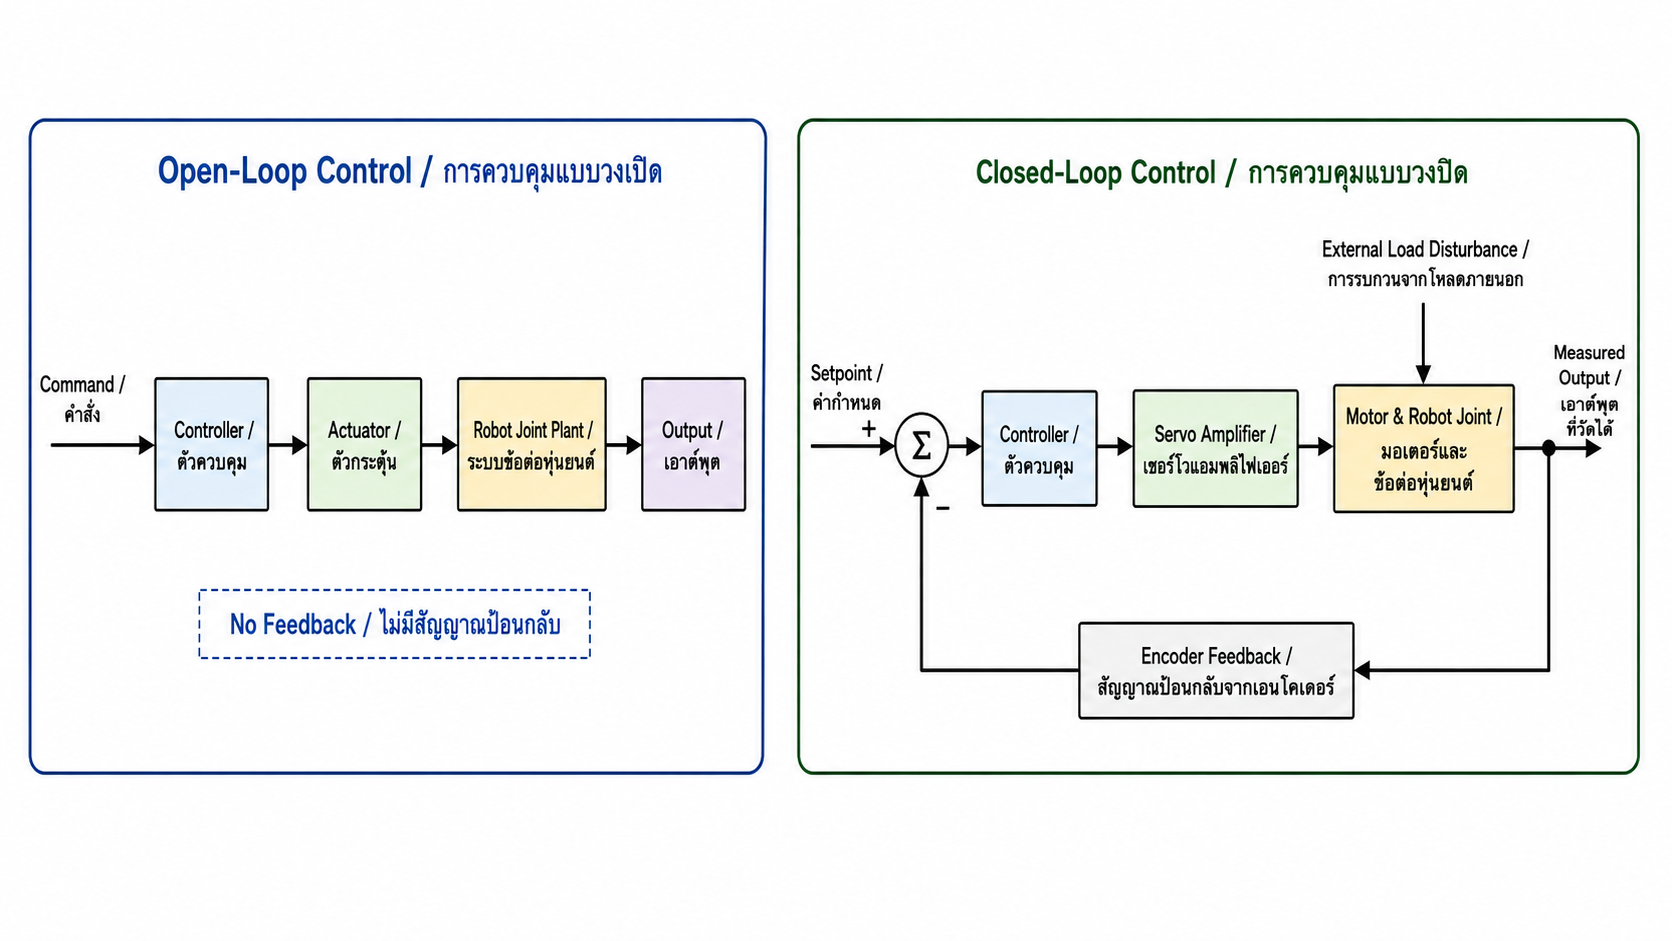
\includegraphics[width=0.8\textwidth]{images/chapter6/figure-01.png}
    \caption{การเปรียบเทียบระบบควบคุมวงเปิดและวงปิด}
\end{figure}



\subsubsection{ตัวชี้วัดสมรรถนะของผลตอบสนอง}

เมื่อให้คำสั่ง Step ระบบวงปิดมักประเมินด้วยตัวชี้วัดต่อไปนี้

\begin{enumerate}
    \item \textbf{Rise Time ($t_r$):} เวลาที่ผลตอบสนองเพิ่มจากค่าต่ำไปยังช่วงใกล้ค่าปลายทาง เกณฑ์อาจใช้ 10–90\% หรือเกณฑ์อื่น จึงต้องระบุให้ชัด
    \item \textbf{Peak Time ($t_p$):} เวลาที่เกิดค่าสูงสุดครั้งแรก
    \item \textbf{Maximum Overshoot ($M_p$):} ร้อยละที่ผลตอบสนองสูงเกินค่าปลายทาง
    \item \textbf{Settling Time ($t_s$):} เวลาที่ผลตอบสนองเข้าสู่และคงอยู่ในแถบ เช่น $\pm2\%$ หรือ $\pm5\%$
    \item \textbf{Steady-state Error ($e_{ss}$):} Error ที่เหลือเมื่อระบบเข้าสู่สภาวะคงตัว
    \item \textbf{Bandwidth:} ช่วงความถี่ที่ระบบสามารถติดตามคำสั่งหรือปฏิเสธ Disturbance ได้ตามเกณฑ์
    \item \textbf{Stability Margin:} ระยะเผื่อก่อนระบบเข้าสู่ภาวะไม่เสถียร เช่น Gain Margin และ Phase Margin
\end{enumerate}

ค่าพุ่งเกินคำนวณได้โดย

\[
M_p(\%)=\frac{y_{max}-y_{ss}}{y_{ss}}\times100
\]

โดย $y_{max}$ คือค่าสูงสุด และ $y_{ss}$ คือค่าปลายทาง

\paragraph{ตัวอย่างที่ 6.2 การคำนวณ Overshoot}

\textbf{ตัวอย่างเพิ่มเติมเพื่อการเรียนรู้}

ระบบตำแหน่งได้รับคำสั่ง $90^\circ$ วัดค่าสูงสุดได้ $99^\circ$ และเข้าสู่ค่าคงตัว $90^\circ$

\[
M_p=\frac{99-90}{90}\times100=10\%
\]

ผลตอบสนองมี Overshoot เท่ากับ 10\% หากงานเป็นการประกอบใกล้ชิ้นส่วนอื่น ค่า Overshoot นี้อาจมากเกินไปแม้ค่าปลายทางถูกต้อง จึงต้องประเมินทั้ง Transient Response และข้อจำกัดของพื้นที่ทำงาน



\subsubsection{การควบคุมแบบ PID}

ตัวควบคุม PID แบบต่อเนื่องมีรูป

\[
u(t)=K_p e(t)+K_i\int_0^t e(\tau)\,d\tau+K_d\frac{de(t)}{dt}
\]

โดย

\begin{itemize}
    \item $u(t)$ คือคำสั่งควบคุม เช่น กระแสอ้างอิง แรงบิดอ้างอิง หรือความเร็วอ้างอิง
    \item $e(t)$ คือ Error
    \item $K_p$ คือ Proportional Gain
    \item $K_i$ คือ Integral Gain
    \item $K_d$ คือ Derivative Gain
\end{itemize}

หน่วยของ Gain ขึ้นกับหน่วยของ $u$ และ $e$ ตัวอย่างเช่น หาก $u$ มีหน่วยโวลต์และ $e$ มีหน่วยเรเดียน จะได้ $K_p$ หน่วยโวลต์ต่อเรเดียน $K_i$ หน่วยโวลต์ต่อเรเดียนต่อวินาที และ $K_d$ หน่วยโวลต์วินาทีต่อเรเดียน

ในโดเมนลาปลาซ เมื่อสมมติค่าเริ่มต้นเป็นศูนย์

\[
C(s)=K_p+\frac{K_i}{s}+K_ds
\]

\paragraph{7.4.1 พจน์สัดส่วน}

พจน์สัดส่วนสร้างคำสั่งตาม Error ปัจจุบัน

\[
u_P(t)=K_pe(t)
\]

การเพิ่ม $K_p$ มักทำให้ระบบตอบสนองเร็วขึ้นและลด Error แต่หากสูงเกินไปอาจเพิ่ม Overshoot การสั่น และความไวต่อ Noise หรือความหน่วง

\paragraph{7.4.2 พจน์ปริพันธ์}

พจน์ปริพันธ์สะสม Error ตามเวลา

\[
u_I(t)=K_i\int_0^t e(\tau)\,d\tau
\]

จุดเด่นคือกำจัด Steady-state Error สำหรับระบบและคำสั่งบางประเภท แต่ทำให้ Phase Lag เพิ่มและอาจเกิด Overshoot มากขึ้น หาก Actuator อิ่มตัวแต่ Integrator ยังสะสม Error จะเกิด \textbf{Integral Windup}

แนวทางลด Windup ได้แก่

\begin{itemize}
    \item จำกัดค่าของ Integral State
    \item หยุดสะสมเมื่อ Output Saturate และ Error มีทิศทางเพิ่ม Saturation
    \item ใช้ Back-calculation Anti-windup
    \item จำกัดคำสั่งและความเร่งก่อนเข้าสู่ PID
\end{itemize}

\paragraph{7.4.3 พจน์อนุพันธ์}

พจน์อนุพันธ์ตอบสนองต่ออัตราการเปลี่ยนแปลงของ Error

\[
u_D(t)=K_d\frac{de(t)}{dt}
\]

พจน์นี้ช่วยเพิ่ม Damping และลด Overshoot ได้ในหลายระบบ แต่ไวต่อ Noise จึงมักใช้ Derivative Filter แทนอนุพันธ์อุดมคติ เช่น

\[
C_D(s)=K_d\frac{Ns}{s+N}
\]

หรือทำ Derivative จากค่าที่วัดแทน Error เพื่อลด Derivative Kick เมื่อ Setpoint เปลี่ยนฉับพลัน

\paragraph{7.4.4 ผลโดยทั่วไปของการปรับ Gain}

\begin{table}[htbp]
    \centering
    \begin{tabular}{l l l l}
        \hline
        \textbf{ตัวแปรสมรรถนะ} & \textbf{เพิ่ม $K_p$} & \textbf{เพิ่ม $K_i$} & \textbf{เพิ่ม $K_d$} \\
        \hline
        Rise Time & มักลดลง & อาจลดลงเล็กน้อย & เปลี่ยนเล็กน้อย \\
        Overshoot & มักเพิ่มขึ้น & มักเพิ่มขึ้น & มักลดลงเมื่อกรองเหมาะสม \\
        Settling Time & อาจเพิ่มหรือลด & มักเพิ่มหากเกิดการสั่น & มักลดจาก Damping ที่เพิ่ม \\
        Steady-state Error & ลดลง & สามารถกำจัดได้ในเงื่อนไขที่เหมาะสม & ไม่กำจัดโดยตรง \\
        Noise Sensitivity & เพิ่มได้เมื่อ Gain สูง & ไวต่อ Bias ระยะยาว & สูง โดยเฉพาะ Noise ความถี่สูง \\
        Stability Margin & อาจลดลง & มักลดลง & อาจดีขึ้นในช่วงที่ออกแบบเหมาะสม \\
        \hline
    \end{tabular}
\end{table}

\begin{quote}
\textbf{ข้อควรระวัง:} ตารางนี้เป็นแนวโน้มทั่วไป ไม่ใช่กฎตายตัว ผลจริงขึ้นกับ Plant, Sampling Time, Filter, Saturation และโครงสร้างตัวควบคุม
\end{quote}

\paragraph{7.4.5 การปรับ PID แบบเป็นขั้นตอน}

แนวทางเชิงปฏิบัติสำหรับห้องทดลองมีดังนี้

\begin{enumerate}
    \item ตรวจสอบทิศทาง Feedback ให้ถูกต้อง หากกลับขั้วระบบจะเป็น Positive Feedback
    \item จำกัด Output, Speed และ Travel ให้อยู่ในระดับปลอดภัย
    \item เริ่มจาก $K_i=0$ และ $K_d=0$
    \item เพิ่ม $K_p$ ทีละน้อยจนตอบสนองเร็วแต่ยังไม่สั่นต่อเนื่อง
    \item เพิ่ม $K_i$ เพื่อกำจัด Error คงตัว พร้อมติดตาม Overshoot และ Windup
    \item เพิ่ม $K_d$ หรือ Damping Term เพื่อปรับ Transient Response หากสัญญาณวัดมี Noise ต่ำพอ
    \item ทดสอบหลาย Setpoint และหลายโหลด ไม่ใช้ผลจากจุดทำงานเดียว
    \item บันทึก Rise Time, Overshoot, Settling Time, Error และ Peak Control Effort
    \item ตรวจอุณหภูมิ กระแสสูงสุด และ Alarm ของ Drive
    \item ยืนยันผลด้วยการทำซ้ำและกำหนดเกณฑ์ยอมรับ
\end{enumerate}

\paragraph{ตัวอย่างที่ 6.3 การคำนวณเอาต์พุต PID ณ ขณะหนึ่ง}

\textbf{ตัวอย่างเพิ่มเติมเพื่อการเรียนรู้}

กำหนด $K_p=2.0$, $K_i=0.8\ \text{s}^{-1}$, $K_d=0.1\ \text{s}$ ณ เวลาหนึ่งมี Error $e=0.5$ หน่วย Integral Error เท่ากับ $0.3\ \text{unit·s}$ และอัตราการเปลี่ยน Error เท่ากับ $-0.4\ \text{unit/s}$

\[
u=K_pe+K_i\int e\,dt+K_d\frac{de}{dt}
\]

\[
u=2.0(0.5)+0.8(0.3)+0.1(-0.4)
\]

\[
u=1.00+0.24-0.04=1.20
\]

คำตอบคือ $u=1.20$ หน่วยคำสั่ง พจน์ D มีค่าเป็นลบเพราะ Error กำลังลดลง จึงช่วยชะลอการเข้าใกล้ Setpoint และลดแนวโน้ม Overshoot

\paragraph{7.4.6 PID แบบดิจิทัล}

Robot Controller และ Servo Drive ใช้ตัวควบคุมดิจิทัล จึงคำนวณตามรอบ Sampling Time $T_s$ รูปแบบอย่างง่ายคือ

\[
I[k]=I[k-1]+K_iT_se[k]
\]

\[
D[k]=K_d\frac{e[k]-e[k-1]}{T_s}
\]

\[
u[k]=K_pe[k]+I[k]+D[k]
\]

เมื่อ $T_s$ เปลี่ยน ผลของพจน์ I และ D จะเปลี่ยนตาม หากย้ายค่าพารามิเตอร์ระหว่าง Controller ที่ใช้สูตรภายในต่างกัน ต้องตรวจสอบนิยาม Gain ไม่ควรคัดลอกตัวเลขโดยตรงโดยไม่อ่านคู่มือ

%\paragraph{รูปที่ 6.2 PID Response Curves}

% [รูปที่ 6.2: ผลกระทบของค่า PID ต่อ Step Response]
% ประเภทภาพ: Graph
% ตำแหน่งที่แนะนำ: หลังหัวข้อ 7.4
% วัตถุประสงค์การเรียนรู้: แสดงแนวโน้มของ Rise Time, Overshoot, Settling Time และ Steady-state Error เมื่อปรับ Gain
% คำอธิบายภาพ: กราฟสี่ช่องหรือกราฟซ้อนที่เปรียบเทียบ Base Response กับกรณีเพิ่ม Kp, เพิ่ม Ki และเพิ่ม Kd โดยใช้เส้น Setpoint เดียวกัน และกำกับว่าเป็นแนวโน้มเชิงคุณภาพ
% องค์ประกอบที่ต้องมี: แกนเวลา แกนผลตอบสนอง เส้น Setpoint จุด Overshoot และแถบ Settling
% ข้อความหรือป้ายกำกับ: Base, Higher Kp, Higher Ki, Higher Kd, Setpoint, Overshoot, Settling Band
% ภาษาของป้ายกำกับ: ไทยและอังกฤษ
% สัดส่วนภาพ: 16:9
% Graph Generation Prompt: Create an engineering textbook graph illustrating qualitative PID gain effects on a normalized unit-step response. Use four clearly labeled panels: baseline, increased Kp, increased Ki, and increased Kd. Show normalized output y(t) from 0 to 1.5 and time from 0 to 5 seconds. Include a horizontal setpoint at 1.0, mark overshoot and a ±2 percent settling band, and state that curves are conceptual and plant-dependent. Bilingual Thai-English labels, clean white background, 16:9.
% Alt Text: กราฟเชิงแนวคิดแสดงว่าการเพิ่ม Kp และ Ki มักเพิ่มความเร็วและ Overshoot ขณะที่ Kd เพิ่ม Damping แต่ผลจริงขึ้นกับระบบ

\begin{figure}[htbp]
    \centering
    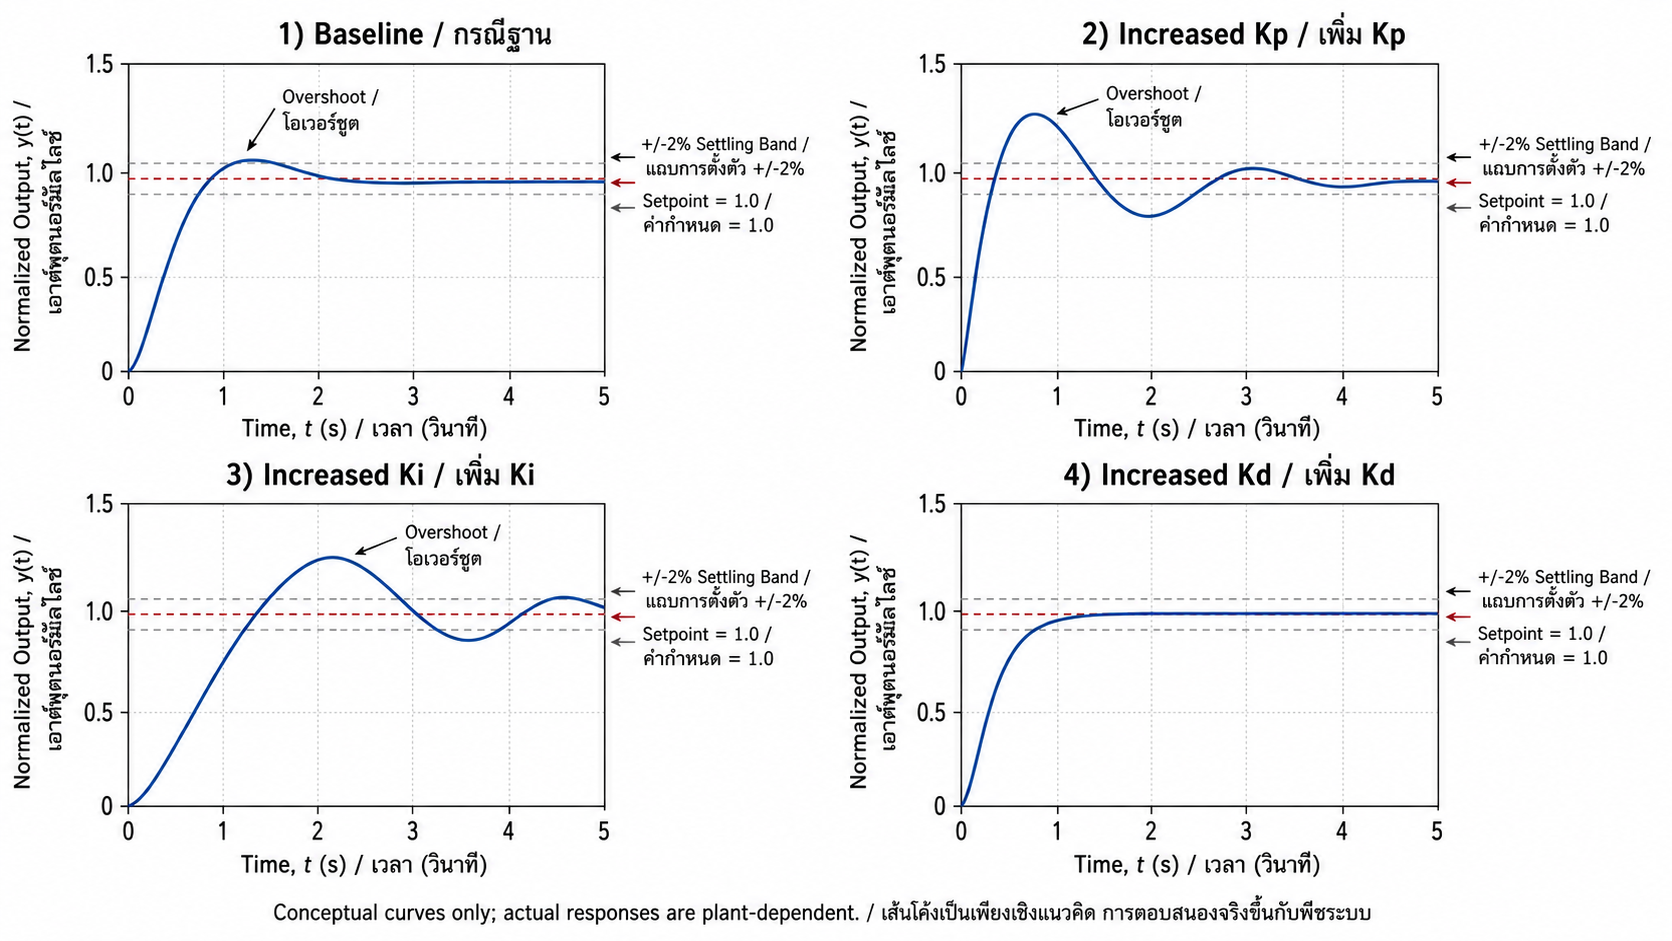
\includegraphics[width=0.8\textwidth]{images/chapter6/figure-02.png}
    \caption{ผลกระทบของค่า PID ต่อ Step Response}
\end{figure}



\subsubsection{การควบคุมตำแหน่ง ความเร็ว และแรงบิด}

Servo Drive สมัยใหม่มักรองรับหลายโหมดควบคุม แต่ละโหมดมีตัวแปรควบคุมและการใช้งานแตกต่างกัน

\paragraph{7.5.1 Position Control}

Position Control มีเป้าหมายให้ตำแหน่งจริง $q(t)$ ติดตามตำแหน่งคำสั่ง $q_d(t)$

\[
e_q(t)=q_d(t)-q(t)
\]

คำสั่งจาก Position Controller มักเป็นความเร็วอ้างอิงหรือแรงบิดอ้างอิง ขึ้นกับสถาปัตยกรรม ตัวอย่างงาน ได้แก่

\begin{itemize}
    \item Point-to-Point Motion
    \item Pick and Place
    \item งานประกอบ
    \item งานเชื่อมตามเส้นทาง
    \item การวางชิ้นงานที่ต้องการ Repeatability สูง
\end{itemize}

Position Control ต้องพิจารณา Motion Profile เพื่อจำกัดความเร็ว ความเร่ง และ Jerk หากเปลี่ยน Setpoint แบบ Step โดยตรง อาจทำให้คำสั่งแรงบิดสูงเกินขีดจำกัด

\paragraph{7.5.2 Speed Control}

Speed Control ให้ความเร็วจริง $\omega(t)$ ติดตามค่าคำสั่ง $\omega_d(t)$

\[
e_\omega(t)=\omega_d(t)-\omega(t)
\]

โหมดนี้ใช้ใน Conveyor, Spindle, Roll Feed และเป็นวงรอบภายในของ Position Control ความเร็วอาจคำนวณจาก Encoder โดยการหาความแตกต่างของตำแหน่งตามเวลา จึงต้องกรอง Noise โดยไม่เพิ่ม Delay มากเกินไป

\paragraph{7.5.3 Torque Control}

ในมอเตอร์ AC Servo ที่ใช้ Field-Oriented Control แรงบิดมีความสัมพันธ์โดยประมาณกับกระแสแกน $q$

\[
\tau_m=K_t i_q
\]

โดย $\tau_m$ คือแรงบิดมอเตอร์ หน่วย N·m, $K_t$ คือ Torque Constant หน่วย N·m/A และ $i_q$ คือกระแสสร้างแรงบิด หน่วย A

Torque Control เหมาะกับ

\begin{itemize}
    \item Force Control และ Contact Task
    \item Press-fit
    \item Screwdriving
    \item Tension Control
    \item Collision Detection บางรูปแบบ
    \item Gravity Compensation
\end{itemize}

อย่างไรก็ตาม แรงบิดมอเตอร์ไม่เท่ากับแรงที่ End Effector โดยตรง เพราะยังมีอัตราทด ประสิทธิภาพ แรงเสียดทาน และพลวัตของกลไก

หากละเลยการสูญเสียและใช้ Jacobian ความสัมพันธ์ระหว่าง Joint Torque กับ Wrench ที่ปลายแขนเขียนได้เป็น

\[
\boldsymbol{\tau}=\mathbf{J}^T(\mathbf{q})\mathbf{F}
\]

โดย $\boldsymbol{\tau}$ เป็นเวกเตอร์แรงบิดข้อต่อ และ $\mathbf{F}$ เป็นเวกเตอร์แรงและโมเมนต์ที่ End Effector

\paragraph{7.5.4 ตารางเลือกโหมดควบคุม}

\begin{table}[htbp]
    \centering
    \small
    \begin{tabularx}{\textwidth}{@{}L{0.12\textwidth} L{0.17\textwidth} L{0.14\textwidth} X X L{0.14\textwidth}@{}}
        \hline
        \textbf{โหมด} & \textbf{ตัวแปรป้อนกลับหลัก} & \textbf{คำสั่งหลัก} & \textbf{จุดเด่น} & \textbf{ข้อควรระวัง} & \textbf{ตัวอย่างงาน} \\
        \hline
        Position & ตำแหน่ง Encoder & Position/Trajectory & แม่นยำ เหมาะกับการเคลื่อนตามจุด & ต้องจำกัด Motion Profile & Pick and Place \\
        Speed & ความเร็วที่วัดหรือประมาณ & Speed & รักษาความเร็วสม่ำเสมอ & Noise จากการคำนวณความเร็ว & Conveyor, Spindle \\
        Torque & Current/Torque Estimate & Torque/Current & ควบคุมแรงสัมผัสได้รวดเร็ว & ต้องจำกัดแรงและจัดการ Gravity/Friction & Press-fit, Tension \\
        \hline
    \end{tabularx}
\end{table}



\subsubsection{โครงสร้างวงรอบซ้อนของ Servo Axis}

ระบบ Servo อุตสาหกรรมมักใช้วงรอบซ้อนดังนี้

\begin{center}
Position Command
$\downarrow$ \\
Position Controller -> Speed Command
$\downarrow$ \\
Speed Controller -> Torque/Current Command
$\downarrow$ \\
Current Controller -> PWM Inverter -> Servo Motor -> Robot Joint
$\downarrow$ \\
Current Sensor      Encoder Speed    Encoder Position
\end{center}

หลักสำคัญคือวงรอบด้านในต้องเร็วกว่าและคงตัวก่อน จึงออกแบบวงรอบด้านนอกได้ โดยทั่วไป

\begin{itemize}
    \item Current Loop เร็วที่สุด
    \item Speed Loop ช้ากว่า Current Loop
    \item Position Loop ช้าที่สุด
\end{itemize}

อัตราส่วน Bandwidth ที่เหมาะสมขึ้นกับระบบและผู้ผลิต ไม่ควรใช้ตัวเลขตายตัว แต่แนวปฏิบัติคือแยก Bandwidth แต่ละวงให้ห่างพอเพื่อลดปฏิสัมพันธ์

หากกำหนด Bandwidth โดยประมาณเป็น $f_i$, $f_v$ และ $f_p$ สำหรับ Current, Velocity และ Position Loop ตามลำดับ ควรมี

\[
f_i>f_v>f_p
\]

แนวทางเริ่มต้นเพื่อการศึกษาอาจใช้

\[
f_i\approx 5f_v, \qquad f_v\approx 5f_p
\]

แต่ต้องยืนยันกับ Plant จริงและคู่มือ Drive

\paragraph{ตัวอย่างที่ 6.4 การกำหนด Bandwidth เริ่มต้น}

\textbf{ตัวอย่างเพิ่มเติมเพื่อการเรียนรู้}

กำหนด Current Loop Bandwidth $f_i=1000\ \text{Hz}$ ต้องการกำหนดค่าเริ่มต้นของ Speed และ Position Loop ด้วยอัตราส่วน 5:1

\[
f_v=\frac{1000}{5}=200\ \text{Hz}
\]

\[
f_p=\frac{200}{5}=40\ \text{Hz}
\]

ค่าดังกล่าวเป็นเพียงจุดเริ่มต้น การใช้งานจริงต้องพิจารณา Resonance ของกลไก Sampling Frequency ความแข็งของ Gearbox และ Filter

\paragraph{7.6.1 Following Error}

Following Error คือผลต่างระหว่างตำแหน่งคำสั่งกับตำแหน่งจริง

\[
e_f(t)=q_d(t)-q(t)
\]

Robot Controller มักกำหนดขีดจำกัด Following Error หากเกินค่าที่กำหนดจะเกิด Alarm เพื่อป้องกันการเคลื่อนที่ผิดปกติ สาเหตุอาจมาจาก

\begin{itemize}
    \item โหลดมากเกินไป
    \item กลไกติดขัด
    \item Gain ต่ำหรือสูงไม่เหมาะสม
    \item Encoder Fault
    \item Motor Phase หรือ Brake ผิดปกติ
    \item Command Profile รุนแรงเกินไป
\end{itemize}

%\paragraph{รูปที่ 6.3 Cascade Control Block Diagram}

% [รูปที่ 6.3: โครงสร้างวงรอบซ้อน Position–Speed–Current]
% ประเภทภาพ: Block Diagram
% ตำแหน่งที่แนะนำ: หลังหัวข้อ 7.6
% วัตถุประสงค์การเรียนรู้: อธิบายความสัมพันธ์ของวงรอบตำแหน่ง ความเร็ว และกระแสใน Servo Drive
% คำอธิบายภาพ: แสดง Position Controller สร้าง Speed Reference, Speed Controller สร้าง Current/Torque Reference และ Current Controller ควบคุม PWM Inverter พร้อม Feedback จาก Encoder และ Current Sensor
% องค์ประกอบที่ต้องมี: Position command, Position loop, Speed loop, Current loop, PWM inverter, servo motor, gearbox, robot joint, encoder, current sensors, bandwidth labels
% ข้อความหรือป้ายกำกับ: Outer Loop, Inner Loop, Fastest Loop, Position Feedback, Speed Feedback, Current Feedback
% ภาษาของป้ายกำกับ: ไทยและอังกฤษ
% สัดส่วนภาพ: 16:9
% Image Generation Prompt: Detailed clean cascade control block diagram for an industrial robot servo axis. Show position command to position controller, speed command to speed controller, torque/current command to current controller, PWM inverter, servo motor, gearbox, and robot joint. Include encoder position feedback, calculated speed feedback, phase current sensors, and arrows. Label current loop as fastest, speed loop as intermediate, position loop as outer and slowest. Engineering textbook vector style, bilingual Thai-English labels, white background, 16:9.
% Alt Text: แผนภาพวงรอบซ้อนที่ Current Loop อยู่ด้านในสุด ตามด้วย Speed Loop และ Position Loop อยู่ด้านนอก

\begin{figure}[htbp]
    \centering
    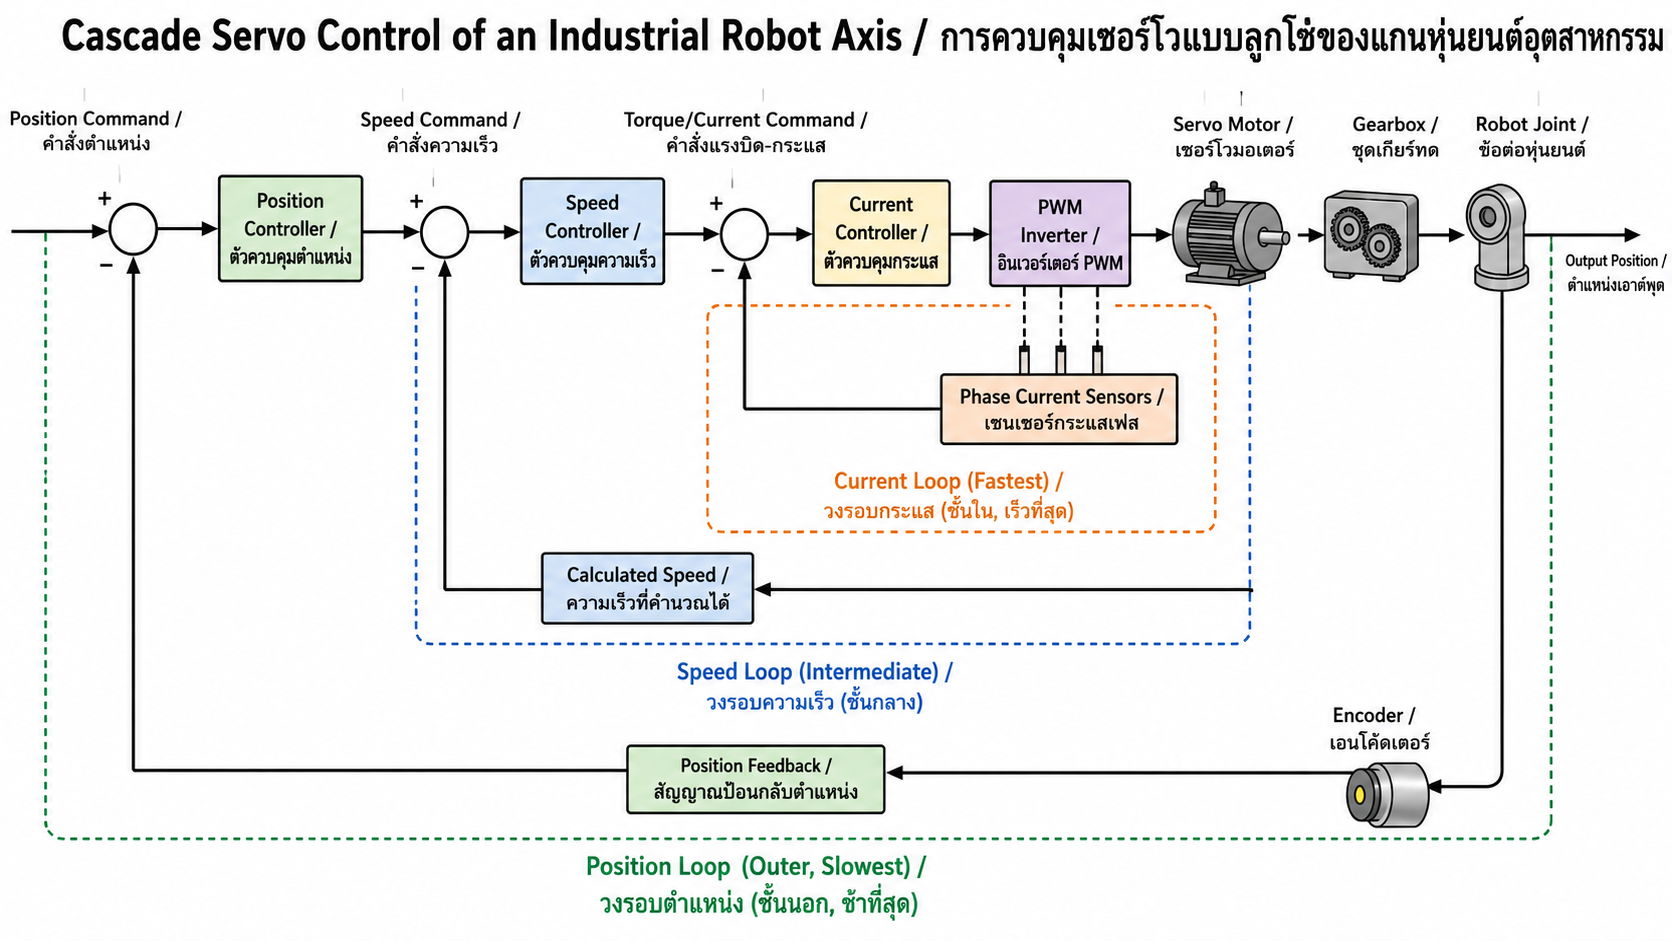
\includegraphics[width=0.8\textwidth]{images/chapter6/figure-03.png}
    \caption{โครงสร้างวงรอบซ้อน Position–Speed–Current}
\end{figure}



\subsubsection{การควบคุมใน Joint Space และ Cartesian Space}

\paragraph{7.7.1 Joint Space Control}

Joint Space Control ควบคุมตัวแปรข้อต่อโดยตรง

\[
\mathbf{q}=\begin{bmatrix}q_1&q_2&\cdots&q_n\end{bmatrix}^T
\]

สำหรับหุ่นยนต์ข้อต่อหมุน $q_i$ คือมุม สำหรับข้อต่อเลื่อน $q_i$ คือระยะทาง วิธีนี้เหมาะกับ Point-to-Point Motion เพราะสามารถวางแผนโปรไฟล์ของแต่ละแกนแล้วให้ทุกแกนถึงเป้าหมายพร้อมกัน

\textbf{ข้อดี}

\begin{itemize}
    \item สอดคล้องกับตัวแปรที่ Servo Controller วัดโดยตรง
    \item คำนวณง่ายกว่า Cartesian Control
    \item เหมาะกับการเคลื่อนที่ที่ไม่กำหนดเส้นทางปลายแขนอย่างเข้มงวด
\end{itemize}

\textbf{ข้อจำกัด}

\begin{itemize}
    \item เส้นทางของ End Effector อาจไม่เป็นเส้นตรง
    \item ต้องใช้ Inverse Kinematics เพื่อแปลงเป้าหมาย Cartesian เป็น Joint Coordinates
    \item ใกล้ Singular Configuration การเปลี่ยนตำแหน่งเล็กน้อยอาจต้องใช้ความเร็วข้อต่อสูง
\end{itemize}

\paragraph{7.7.2 Cartesian Space Control}

กำหนด Pose ของ End Effector เป็น

\[
\mathbf{x}=\begin{bmatrix}x&y&z&\phi&\theta&\psi\end{bmatrix}^T
\]

ความสัมพันธ์เชิงความเร็วคือ

\[
\dot{\mathbf{x}}=\mathbf{J}(\mathbf{q})\dot{\mathbf{q}}
\]

หาก Jacobian มี Inverse ที่เหมาะสม

\[
\dot{\mathbf{q}}=\mathbf{J}^{-1}(\mathbf{q})\dot{\mathbf{x}}
\]

สำหรับหุ่นยนต์ที่ไม่เป็นเมทริกซ์จัตุรัสหรืออยู่ใกล้ Singular มักใช้ Pseudoinverse

\[
\dot{\mathbf{q}}=\mathbf{J}^{\dagger}(\mathbf{q})\dot{\mathbf{x}}
\]

Cartesian Control เหมาะกับงานที่ต้องควบคุมเส้นทางหรือแรงในพิกัดงาน เช่น เชื่อม เจียร ขัดผิว และประกอบชิ้นส่วน

\paragraph{7.7.3 Singularities}

Singularity คือสภาวะที่หุ่นยนต์สูญเสียความสามารถในการสร้างความเร็วหรือแรงในบางทิศทาง หรือจำเป็นต้องใช้ความเร็วข้อต่อสูงมากเพื่อให้ได้ความเร็ว Cartesian ที่กำหนด ใกล้ Singularity ค่าของ $\mathbf{J}^{-1}$ อาจมีขนาดสูงและไวต่อ Noise

แนวทางจัดการ ได้แก่

\begin{itemize}
    \item หลีกเลี่ยงเส้นทางใกล้ Singularity
    \item จำกัด Joint Speed
    \item ใช้ Damped Least Squares Pseudoinverse
    \item เปลี่ยนท่าทางของ Tool หรือ Workpiece
    \item วางตำแหน่งฐานหุ่นยนต์ให้ Workspace เหมาะสม
\end{itemize}

\paragraph{7.7.4 Computed Torque Control}

พลวัตของหุ่นยนต์เขียนได้เป็น

\[
\mathbf{M}(\mathbf{q})\ddot{\mathbf{q}}+\mathbf{C}(\mathbf{q},\dot{\mathbf{q}})\dot{\mathbf{q}}+\mathbf{g}(\mathbf{q})+\mathbf{f}(\dot{\mathbf{q}})=\boldsymbol{\tau}
\]

โดย

\begin{itemize}
    \item $\mathbf{M}(\mathbf{q})$ คือ Inertia Matrix
    \item $\mathbf{C}(\mathbf{q},\dot{\mathbf{q}})\dot{\mathbf{q}}$ คือ Coriolis และ Centrifugal Term
    \item $\mathbf{g}(\mathbf{q})$ คือ Gravity Term
    \item $\mathbf{f}(\dot{\mathbf{q}})$ คือ Friction
    \item $\boldsymbol{\tau}$ คือ Joint Torque
\end{itemize}

Computed Torque Control ใช้แบบจำลองชดเชย Nonlinear Dynamics แล้วกำหนด Tracking Error Dynamics ที่ต้องการ รูปหนึ่งคือ

\[
\boldsymbol{\tau}=\mathbf{M}(\mathbf{q})\left[\ddot{\mathbf{q}}_d+\mathbf{K}_d(\dot{\mathbf{q}}_d-\dot{\mathbf{q}})+\mathbf{K}_p(\mathbf{q}_d-\mathbf{q})\right]
+\mathbf{C}(\mathbf{q},\dot{\mathbf{q}})\dot{\mathbf{q}}+\mathbf{g}(\mathbf{q})
\]

เมื่อแบบจำลองแม่นยำ ระบบ Error จะมีพฤติกรรมใกล้เคียงระบบเชิงเส้นอันดับสอง แต่ความคลาดเคลื่อนของมวล Payload แรงเสียดทาน และความยืดหยุ่นทำให้ประสิทธิภาพลดลง จึงอาจต้องใช้ Robust หรือ Adaptive Compensation

\paragraph{ตัวอย่างที่ 6.5 Gravity Compensation ของข้อต่อเดียว}

\textbf{ตัวอย่างเพิ่มเติมเพื่อการเรียนรู้}

แขนข้อต่อเดียวมีมวลรวม $m=5\ \text{kg}$ จุดศูนย์กลางมวลอยู่ห่างแกน $l=0.25\ \text{m}$ และแขนทำมุม $\theta=60^\circ$ วัดจากแนวดิ่ง กำหนด $g=9.81\ \text{m/s}^2$

แรงบิดโน้มถ่วงคือ

\[
\tau_g=mgl\sin\theta
\]

\[
\tau_g=5(9.81)(0.25)\sin60^\circ
\]

\[
\tau_g\approx10.62\ \text{N·m}
\]

Controller ต้องสร้างแรงบิดอย่างน้อยประมาณ $10.62\ \text{N·m}$ เพื่อคงตำแหน่งในแบบจำลองอุดมคติ และต้องเผื่อแรงเสียดทาน การเร่ง และประสิทธิภาพชุดส่งกำลังในระบบจริง



\subsubsection{การเชื่อมต่อ PLC กับ Robot Controller}

PLC ทำหน้าที่ควบคุมลำดับงานระดับเซลล์ ขณะที่ Robot Controller จัดการ Motion Planning และ Servo Control การแบ่งหน้าที่ที่ชัดเจนช่วยลดความซับซ้อนและทำให้วินิจฉัยปัญหาง่าย

\paragraph{7.8.1 Digital I/O แบบเดินสายตรง}

ตัวอย่างสัญญาณจาก PLC ไป Robot Controller

\begin{itemize}
    \item Cycle Start
    \item Cycle Stop หรือ Hold
    \item Reset Fault
    \item Program Select Bits
    \item Part Present
    \item Fixture Clamped
    \item Permission to Enter
    \item Automatic Mode Request
\end{itemize}

ตัวอย่างสัญญาณจาก Robot Controller ไป PLC

\begin{itemize}
    \item Robot Ready
    \item Servo On Status
    \item Running
    \item Program Complete
    \item At Home
    \item At Maintenance Position
    \item Gripper Open/Closed
    \item Fault Present
    \item Fault Code Bits
\end{itemize}

\begin{quote}
\textbf{ข้อสำคัญด้านความปลอดภัย:} Emergency Stop, Guard Door และฟังก์ชัน Safety ต้องใช้วงจรหรือเครือข่ายที่มีระดับความปลอดภัยเหมาะสม เช่น Safety Relay, Safety PLC, Dual-channel Safety I/O หรือ Safety Protocol ตามการประเมินความเสี่ยง ไม่ควรนำ E-Stop ผ่าน Standard PLC I/O เพียงอย่างเดียว
\end{quote}

\paragraph{7.8.2 Source/Sink และ PNP/NPN}

การต่อ Digital I/O ต้องตรวจสอบชนิดเอาต์พุตและอินพุต

\begin{itemize}
    \item \textbf{PNP Output:} จ่ายแรงดันบวกให้โหลดเมื่อ ON มักเรียก Sourcing Output
    \item \textbf{NPN Output:} ดึงกระแสลง 0 V เมื่อ ON มักเรียก Sinking Output
\end{itemize}

หาก PLC และ Robot I/O ใช้ Logic ไม่เข้ากัน อาจใช้ Interposing Relay, Optocoupler หรือ Interface Module การต่อ Common Reference ผิดอาจทำให้สัญญาณไม่ทำงานหรือทำให้อุปกรณ์เสียหาย

\paragraph{7.8.3 Handshake Sequence}

การส่ง Pulse Start เพียงเส้นเดียวอาจทำให้เกิด Race Condition หรือคำสั่งสูญหาย จึงควรใช้ Handshake ตัวอย่างลำดับคือ

\begin{enumerate}
    \item PLC ตรวจสอบ Robot Ready และ Cell Safe
    \item PLC กำหนด Program Number
    \item PLC เปิดสัญญาณ Start Request
    \item Robot ตรวจ Program Number และตอบ Start Acknowledge
    \item PLC ปิด Start Request
    \item Robot ปิด Start Acknowledge และเริ่มทำงาน
    \item Robot เปิด Running
    \item เมื่อจบงาน Robot เปิด Complete
    \item PLC รับ Complete และปิดเงื่อนไขรอบงาน
    \item Robot ปิด Complete เมื่อได้รับ Acknowledge หรือเมื่อเงื่อนไข Reset ครบ
\end{enumerate}

ควรกำหนด Timeout ทุกขั้นตอน หากไม่ได้รับ Acknowledge ภายในเวลาที่กำหนด PLC ต้องเข้าสู่สถานะ Fault หรือ Recovery ที่ปลอดภัย

\paragraph{7.8.4 การเลือก Program ด้วย Bit}

หากใช้ $n$ บิต จะเลือกหมายเลขโปรแกรมได้สูงสุด

\[
N=2^n
\]

ตัวอย่างใช้ 4 บิตเลือกได้ 16 ค่า ตั้งแต่ 0 ถึง 15 แต่ควรกำหนดบางรหัสไว้สำหรับ No Program, Maintenance หรือ Invalid Code

\paragraph{ตัวอย่างที่ 6.6 การออกแบบ Program Select}

ต้องการเลือกโปรแกรมการผลิต 10 โปรแกรม

หา $n$ ที่ทำให้

\[
2^n\ge10
\]

เมื่อ $n=3$ จะได้ 8 ค่า ไม่เพียงพอ เมื่อ $n=4$ จะได้ 16 ค่า จึงต้องใช้ Program Select อย่างน้อย 4 บิต

\paragraph{7.8.5 Analog I/O}

Analog I/O ใช้ส่งค่าต่อเนื่อง เช่น

\begin{itemize}
    \item Speed Reference 0–10 V
    \item Force/Torque Reference ±10 V
    \item Process Value 4–20 mA
    \item Pressure หรือ Flow Feedback
\end{itemize}

ข้อดีของ 4–20 mA คือสามารถตรวจจับสายขาดได้เมื่อกระแสต่ำกว่า 4 mA และทน Noise ในระยะไกลได้ดีกว่าสัญญาณแรงดันในหลายสภาพแวดล้อม

การแปลงสเกลแบบเชิงเส้นจากกระแส $I$ ช่วง 4–20 mA ไปยังค่ากระบวนการ $x$ ช่วง $x_{min}$ ถึง $x_{max}$ คือ

\[
x=x_{min}+\frac{I-4}{16}(x_{max}-x_{min})
\]

\paragraph{ตัวอย่างที่ 6.7 การแปลง 4–20 mA เป็นแรงบิด}

Torque Sensor กำหนดช่วง 4–20 mA เท่ากับ 0–200 N·m วัดได้ 12 mA

\[
\tau=0+\frac{12-4}{16}(200-0)
\]

\[
\tau=100\ \text{N·m}
\]

%\paragraph{รูปที่ 6.4 Robot–PLC I/O Wiring}

% [รูปที่ 6.4: การต่อ PLC กับ Robot Controller ผ่าน Hard-wired I/O]
% ประเภทภาพ: Technical Illustration / Wiring Diagram
% ตำแหน่งที่แนะนำ: หลังหัวข้อ 7.8
% วัตถุประสงค์การเรียนรู้: แสดงการแยก Standard I/O, Analog I/O และ Safety Circuit
% คำอธิบายภาพ: PLC Standard Output ต่อไปยัง Robot Standard Input ผ่าน Interface Relay; Robot Output ต่อกลับ PLC Input; Analog 4–20 mA แยก Shield; E-Stop และ Guard Door ผ่าน Safety Relay หรือ Safety PLC แบบสองช่องสัญญาณไปยัง Safety Interface ของ Robot
% องค์ประกอบที่ต้องมี: 24 VDC supply, fuse, PLC I/O, robot controller I/O, terminal blocks, interposing relays, common 0 V, shield grounding, safety relay, dual-channel E-stop, guard switch
% ข้อความหรือป้ายกำกับ: Standard Control, Safety-rated Circuit, Do Not Route E-stop Through Standard I/O Only
% ภาษาของป้ายกำกับ: ไทยและอังกฤษ
% สัดส่วนภาพ: 16:9
% Image Generation Prompt: Safe educational wiring diagram of a PLC connected to an industrial robot controller. Show 24 VDC standard digital outputs and inputs through terminal blocks and interposing relays for Start, Reset, Ready, Running, Complete and Fault. Show a separate shielded 4–20 mA analog channel. Clearly separate a dual-channel emergency-stop and guard-door circuit through a safety relay or safety PLC to the robot safety interface. Include fuses, common 0 V, protective earth, cable shields, and warning that emergency stop must not rely on standard PLC I/O alone. Clean engineering textbook vector style, bilingual labels, white background, 16:9.
% Alt Text: แผนผังต่อสาย PLC กับ Robot Controller ที่แยกวงจรควบคุมปกติออกจากวงจร Safety แบบสองช่องสัญญาณ

\begin{figure}[htbp]
    \centering
    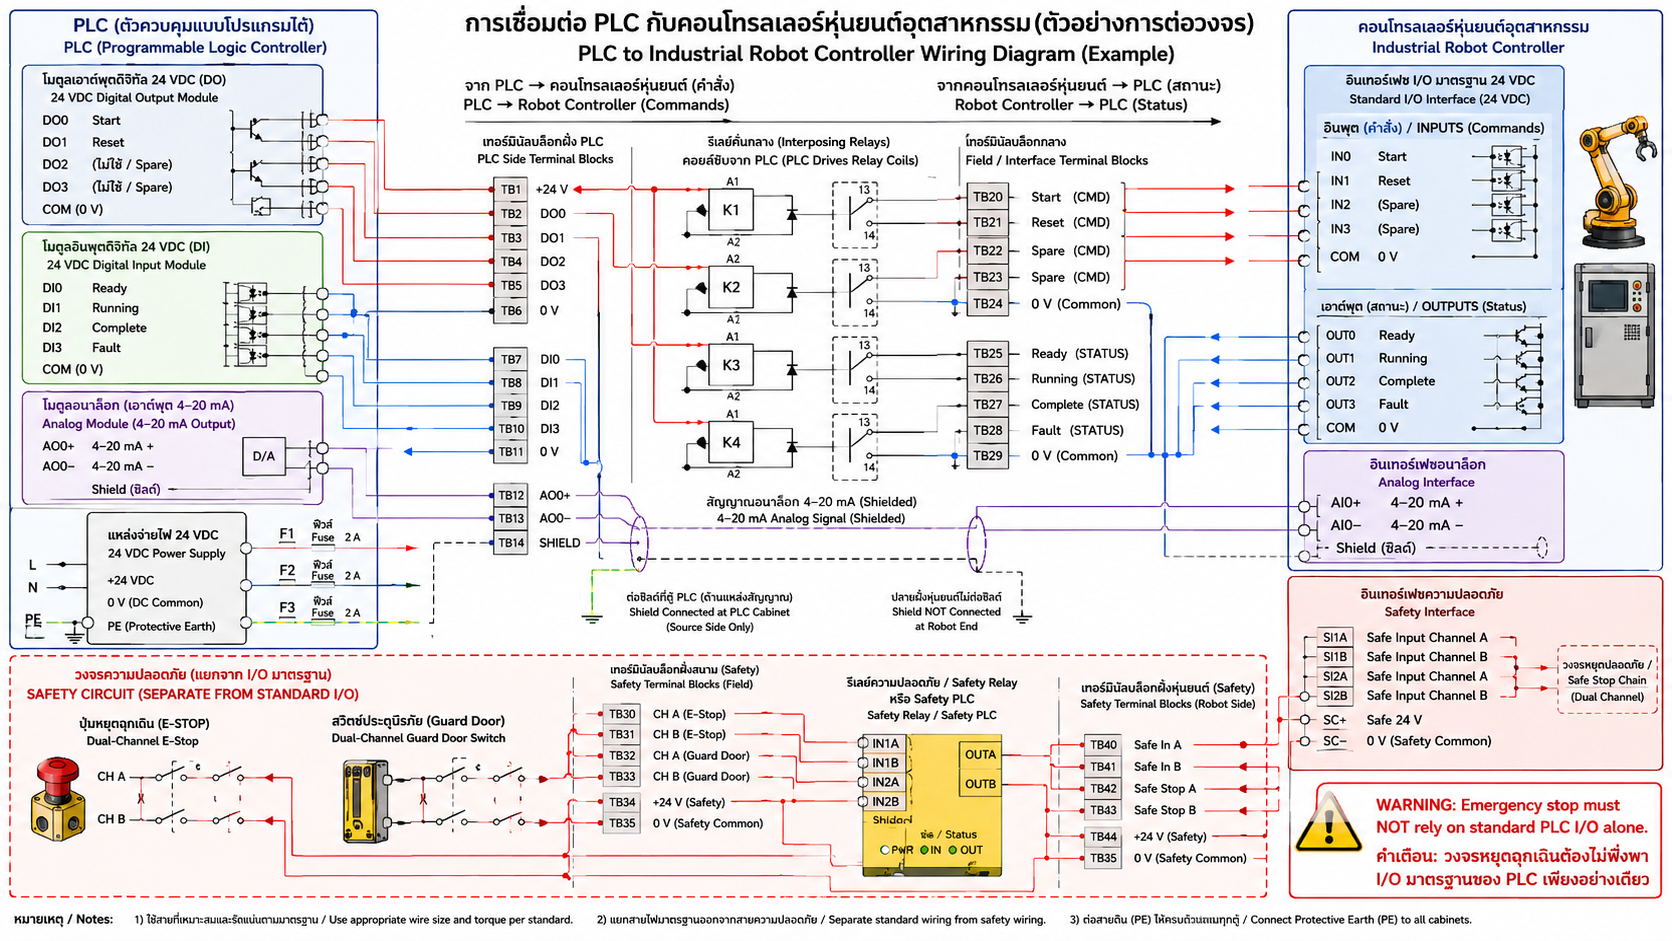
\includegraphics[width=0.8\textwidth]{images/chapter6/figure-04.png}
    \caption{การต่อ PLC กับ Robot Controller ผ่าน Hard-wired I/O}
\end{figure}



\subsubsection{ระดับการบูรณาการ Robot–PLC}

\begin{table}[htbp]
    \centering
    \small
    \begin{tabularx}{\textwidth}{@{}L{0.07\textwidth} L{0.15\textwidth} X L{0.13\textwidth} X X@{}}
        \hline
        \textbf{ระดับ} & \textbf{วิธีการ} & \textbf{ลักษณะข้อมูล} & \textbf{ความซับซ้อน} & \textbf{จุดเด่น} & \textbf{ข้อจำกัด} \\
        \hline
        1 & Hard-wired I/O & บิตสถานะและคำสั่ง & ต่ำ & เข้าใจง่าย แยกปัญหาง่าย & สายจำนวนมาก ข้อมูลจำกัด \\
        2 & Serial Fieldbus & Cyclic I/O และ Parameter บางส่วน & ปานกลาง & ลดสาย รองรับหลายอุปกรณ์ & Bandwidth และ Diagnostics จำกัดกว่าระบบใหม่ \\
        3 & Industrial Ethernet & Cyclic I/O, Acyclic, Diagnostics & ปานกลางถึงสูง & เร็ว ยืดหยุ่น จัดการข้อมูลมาก & ต้องออกแบบ Switch, Address และ Network Load \\
        4 & OPC UA / Middleware / ROS-Industrial & Semantic Data, Services, Integration & สูง & เชื่อมระดับเครื่องถึงระบบข้อมูล & ไม่แทน Hard Real-time Servo Loop หรือ Safety โดยอัตโนมัติ \\
        \hline
    \end{tabularx}
\end{table}

OPC UA เหมาะกับการแลกเปลี่ยนข้อมูลที่มีโครงสร้าง การวินิจฉัย Recipe และการเชื่อม MES/SCADA ส่วน ROS-Industrial สนับสนุนการเชื่อมอุปกรณ์หุ่นยนต์และความสามารถระดับสูง เช่น Perception และ Motion Planning แต่การนำไปใช้ในโรงงานยังต้องออกแบบ Layer สำหรับ Real-time, Safety และการบำรุงรักษาให้เหมาะสม



\subsubsection{7.10 แนวคิดพื้นฐานของการสื่อสารอุตสาหกรรม}

การประเมินเครือข่ายสำหรับงานควบคุมไม่ควรพิจารณาเพียงอัตราส่งข้อมูลเป็น Mbps แต่ต้องพิจารณาคุณลักษณะด้านเวลาและความน่าเชื่อถือด้วย

\paragraph{7.10.1 Throughput, Cycle Time, Latency และ Jitter}

\begin{itemize}
    \item \textbf{Link Speed:} อัตราสัญญาณของ Physical Link เช่น 100 Mbps หรือ 1 Gbps
    \item \textbf{Throughput:} ปริมาณข้อมูลใช้งานจริงต่อเวลา หลังหัก Overhead และช่วงเวลารอ
    \item \textbf{Cycle Time / Update Time:} เวลาที่ข้อมูล Process Data ถูกแลกเปลี่ยนครบหนึ่งรอบ
    \item \textbf{Latency:} เวลาจากเหตุการณ์ต้นทางจนข้อมูลมีผลที่ปลายทาง
    \item \textbf{Jitter:} ความแปรปรวนของ Cycle Time หรือ Latency
    \item \textbf{Determinism:} ความสามารถในการรับประกันว่าการสื่อสารเสร็จภายในกรอบเวลาที่กำหนด
\end{itemize}

เครือข่าย 1 Gbps อาจมี Latency ที่ไม่แน่นอนหากใช้สวิตช์หรือ Traffic ที่ไม่จัดการ ขณะที่เครือข่ายอัตราต่ำกว่าแต่ออกแบบ Scheduling แบบ Real-time อาจให้ Timing ที่คาดการณ์ได้มากกว่า

\paragraph{7.10.2 Cyclic และ Acyclic Communication}

\textbf{Cyclic Data} ใช้กับ I/O และคำสั่งควบคุมที่ต้องอัปเดตสม่ำเสมอ เช่น Robot Ready, Position Actual และ Torque Command

\textbf{Acyclic Data} ใช้กับ Parameter, Alarm History, Device Identification และ Diagnostic การส่ง Acyclic Traffic ต้องไม่รบกวน Cyclic Control เกินเกณฑ์

\paragraph{7.10.3 การประมาณงบประมาณเวลา}

เวลาตอบสนองรวมของระบบประมาณได้จาก

\[
T_{response}=T_{input}+T_{PLC}+T_{network,out}+T_{robot}+T_{network,in}+T_{output}
\]

โดยแต่ละพจน์อาจมีทั้งค่าเฉลี่ยและค่าสูงสุด การออกแบบงาน Interlock ควรใช้ Worst-case หรือค่าที่ผู้ผลิตรับรอง ไม่ใช้เพียงค่าที่วัดได้หนึ่งครั้ง

\paragraph{ตัวอย่างที่ 6.8 งบประมาณเวลาของ Handshake}

\textbf{ตัวอย่างเพิ่มเติมเพื่อการเรียนรู้}

ระบบมี Input Filter 4 ms, PLC Scan 8 ms, Network Update ไปและกลับด้านละ 4 ms, Robot Task Response 12 ms และ Output Module 4 ms

\[
T_{response}=4+8+4+12+4+4=36\ \text{ms}
\]

ดังนั้น Timeout 20 ms จะสั้นเกินไป แม้ระบบปกติอาจตอบเร็วกว่าในบางรอบ ควรเพิ่ม Margin ตาม Jitter และข้อกำหนดของกระบวนการ เช่นเลือก 100–200 ms สำหรับ Handshake ที่ไม่ใช่ Motion Synchronization ทั้งนี้ต้องทดสอบกับอุปกรณ์จริง



\subsubsection{7.11 แบบจำลอง OSI กับเครือข่ายอุตสาหกรรม}

OSI Model มี 7 ชั้น ได้แก่ Physical, Data Link, Network, Transport, Session, Presentation และ Application โปรโตคอลอุตสาหกรรมจำนวนมากไม่ได้ใช้ทุกชั้นแยกกันอย่างชัดเจน แต่แบบจำลองช่วยแยกปัญหาได้

\begin{table}[htbp]
    \centering
    \begin{tabular}{r l l}
        \hline
        \textbf{ชั้น OSI} & \textbf{หน้าที่โดยย่อ} & \textbf{ตัวอย่างประเด็นในระบบหุ่นยนต์} \\
        \hline
        7 Application & ความหมายของข้อมูลและบริการ & Modbus Function Code, CIP Object, PROFINET I/O Data \\
        6 Presentation & รูปแบบข้อมูล & Byte Order, Data Type, Encoding \\
        5 Session & การจัดการการเชื่อมต่อ & Connection State, Timeout \\
        4 Transport & การส่งปลายทางถึงปลายทาง & TCP, UDP \\
        3 Network & Addressing และ Routing & IP Address, Subnet, Router \\
        2 Data Link & Frame, MAC, Switching, Scheduling & Ethernet Frame, PROFINET RT, EtherCAT Processing \\
        1 Physical & สาย สัญญาณ Connector & RS-485, CAN, 100BASE-TX, Fiber \\
        \hline
    \end{tabular}
\end{table}

Modbus เป็น Application Protocol และสามารถทำงานเหนือ Serial Line หรือ TCP/IP ได้ จึงควรแยกคำว่า “Modbus” ออกจาก Physical Medium เช่น Modbus RTU over RS-485 และ Modbus TCP over Ethernet

%\paragraph{รูปที่ 6.5 OSI Model for Fieldbus}

% [รูปที่ 6.5: การวางโปรโตคอลอุตสาหกรรมบนแบบจำลอง OSI]
% ประเภทภาพ: Infographic / Layer Diagram
% ตำแหน่งที่แนะนำ: หลังหัวข้อ 7.11
% วัตถุประสงค์การเรียนรู้: ช่วยแยก Application Protocol ออกจาก Physical Layer และอธิบายสาเหตุที่โปรโตคอลต่างกันด้านเวลา
% คำอธิบายภาพ: แสดง OSI 7 ชั้น และวาง Modbus RTU, PROFIBUS DP, CANopen, Modbus TCP, EtherNet/IP, PROFINET และ EtherCAT โดยไม่สื่อว่าทุกโปรโตคอลใช้ทุกชั้นเต็มรูปแบบ
% องค์ประกอบที่ต้องมี: ชั้น 1–7, RS-485, CAN, Ethernet, TCP/UDP/IP, Application Objects, Cyclic I/O
% ข้อความหรือป้ายกำกับ: Application Layer, Transport, Network, Data Link, Physical; Serial Fieldbus; Industrial Ethernet
% ภาษาของป้ายกำกับ: ไทยและอังกฤษ
% สัดส่วนภาพ: 16:9
% Image Generation Prompt: Educational OSI model infographic for industrial robot communication. Show seven OSI layers and place representative technologies carefully: RS-485 and CAN at physical/data-link level, PROFIBUS DP and CANopen as fieldbus stacks, Modbus RTU over serial, Modbus TCP over TCP/IP and Ethernet, EtherNet/IP using CIP over standard Ethernet and TCP/UDP/IP, PROFINET with real-time data-link communication and standard Ethernet services, and EtherCAT processing Ethernet frames on the fly. Add a note that mappings are simplified and protocols do not necessarily implement every OSI layer separately. Bilingual Thai-English labels, clean engineering vector style, 16:9.
% Alt Text: อินโฟกราฟิก OSI 7 ชั้นที่เปรียบเทียบ Fieldbus และ Industrial Ethernet พร้อมแยก Physical Medium ออกจาก Application Protocol

\begin{figure}[htbp]
    \centering
    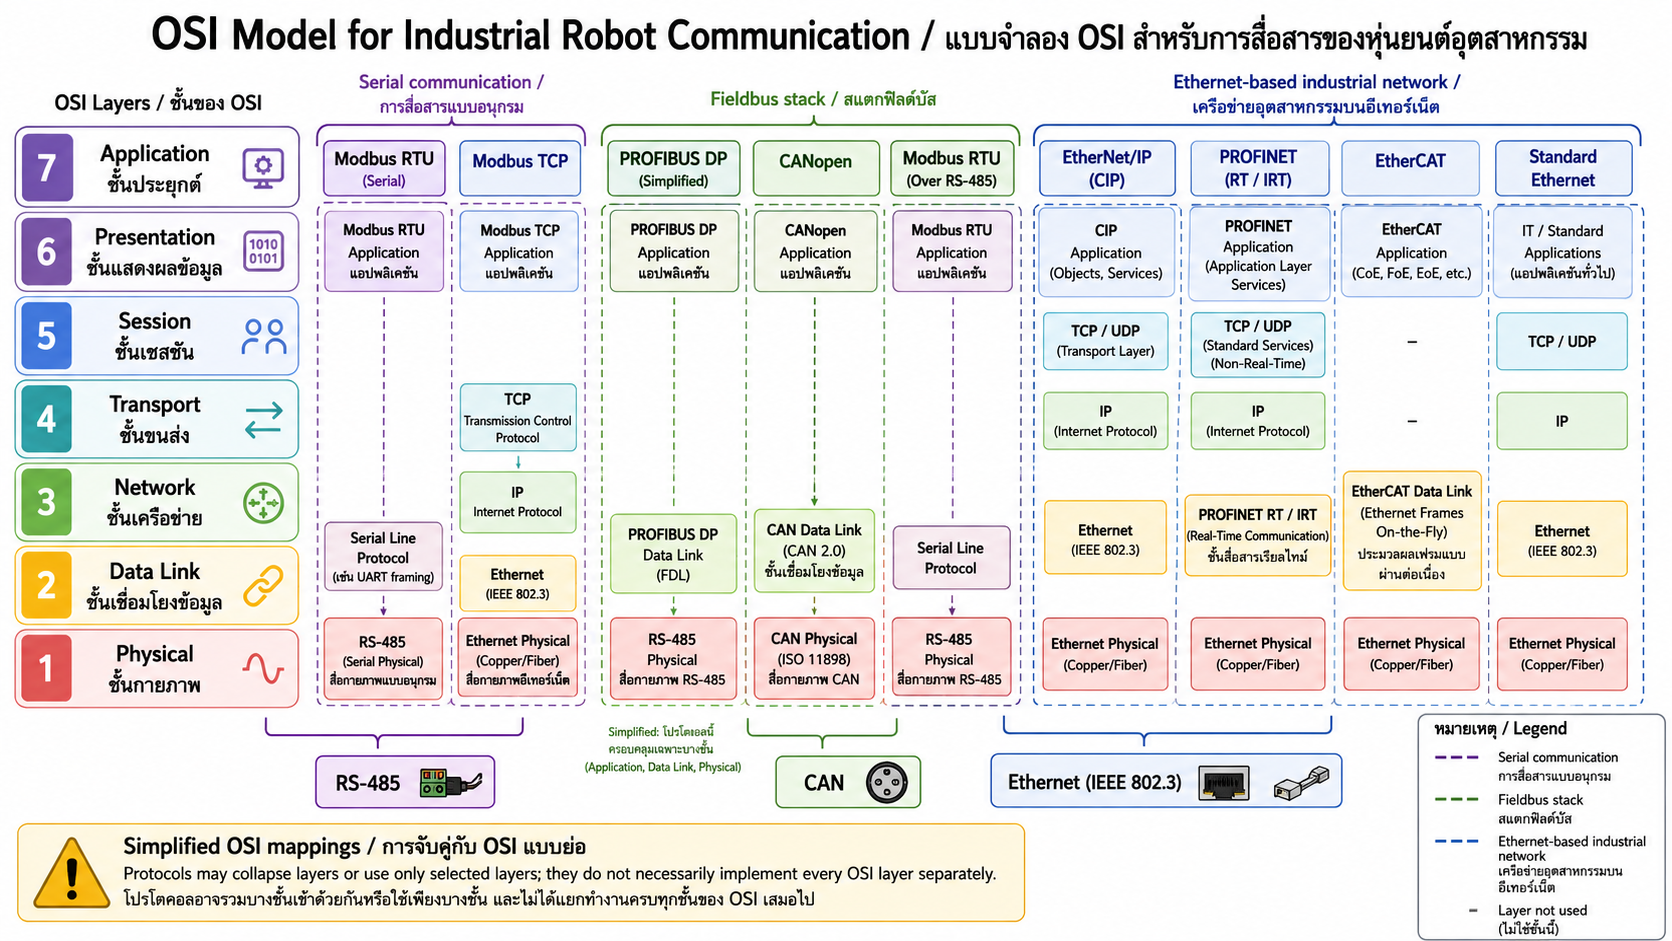
\includegraphics[width=0.8\textwidth]{images/chapter6/figure-05.png}
    \caption{การวางโปรโตคอลอุตสาหกรรมบนแบบจำลอง OSI}
\end{figure}



\subsubsection{Fieldbus ที่ใช้ในระบบหุ่นยนต์}

\paragraph{7.12.1 Modbus RTU}

Modbus RTU เป็นรูปแบบการส่งข้อความ Modbus บน Serial Line มักใช้ RS-485 แบบ Multi-drop โครงสร้างข้อมูลอิง Address และ Function Code เช่น Read Coils, Read Holding Registers และ Write Multiple Registers

\textbf{จุดเด่น}

\begin{itemize}
    \item โครงสร้างไม่ซับซ้อน
    \item มีอุปกรณ์รองรับจำนวนมาก
    \item เหมาะกับ I/O, Meter และอุปกรณ์ Legacy
\end{itemize}

\textbf{ข้อจำกัด}

\begin{itemize}
    \item ไม่มี Semantic Model ที่ละเอียด
    \item การวินิจฉัยและการกำหนดอุปกรณ์ขึ้นกับผู้ผลิต
    \item Timing ขึ้นกับ Baud Rate จำนวนอุปกรณ์ และ Polling Strategy
    \item ต้องจัดการ Byte/Word Order ให้ตรงกัน
\end{itemize}

อัตราส่ง 115.2 kbps พบได้ในอุปกรณ์หลายรุ่น แต่ไม่ใช่ค่าที่รับรองเหมือนกันทุกอุปกรณ์ ระยะสาย RS-485 ที่ยาวต้องลด Baud Rate ใช้สายและ Termination ที่เหมาะสม

\paragraph{7.12.2 PROFIBUS DP}

PROFIBUS DP เป็น Fieldbus สำหรับ Distributed I/O และอุปกรณ์ Automation รองรับอัตราส่งตั้งแต่ 9.6 kbps ถึง 12 Mbps ระยะทางต่อ Segment ลดลงเมื่อ Baud Rate สูงขึ้น ตัวอย่างตามแนวทาง PI คือประมาณ 1,200 m ที่อัตราต่ำ และประมาณ 100 m ที่ 3–12 Mbps เมื่อใช้สายทองแดง Type A ตามข้อกำหนด

\textbf{จุดเด่น}

\begin{itemize}
    \item ระบบนิเวศขนาดใหญ่ในโรงงานเดิม
    \item Cyclic I/O แบบ Master–Device
    \item มีไฟล์ GSD สำหรับ Configuration
\end{itemize}

\textbf{ข้อจำกัด}

\begin{itemize}
    \item ต้องติดตั้ง Termination และ Shield อย่างถูกต้อง
    \item การขยายหรือแก้ปัญหาต้องมีเครื่องมือเฉพาะ
    \item Bandwidth ต่ำกว่า Industrial Ethernet รุ่นใหม่
\end{itemize}

\paragraph{7.12.3 DeviceNet}

DeviceNet ใช้ Common Industrial Protocol (CIP) บน CAN เหมาะกับอุปกรณ์ระดับ Field Device อัตราส่งทั่วไป 125, 250 และ 500 kbps ระยะ Trunk ที่รองรับลดลงเมื่ออัตราส่งสูงขึ้น เช่นประมาณ 500 m ที่ 125 kbps และประมาณ 100 m ที่ 500 kbps ตามข้อกำหนดระบบ

\textbf{จุดเด่น}

\begin{itemize}
    \item ส่ง Power และ Communication ในสายระบบเดียวตามการออกแบบ
    \item ใช้ CIP Object Model
    \item เหมาะกับ Sensor, Valve Island และ Motor Starter รุ่นเดิม
\end{itemize}

\paragraph{7.12.4 CANopen}

CANopen เป็น Higher-layer Protocol บน CAN พัฒนาสำหรับ Embedded Control และ Motion-oriented Machine Control มี Object Dictionary, Process Data Object (PDO), Service Data Object (SDO), Network Management และ Device Profile

CiA 402 กำหนดพฤติกรรมมาตรฐานของ Servo Drive, Frequency Inverter และ Stepper Drive รวมถึง State Machine และ Operation Modes จึงพบใน Robot Joint, AGV และเครื่องจักรขนาดกะทัดรัด

\textbf{จุดเด่น}

\begin{itemize}
    \item มี Device Profile สำหรับ Motion
    \item Configurable และใช้ทรัพยากรไม่สูง
    \item เหมาะกับเครือข่ายภายในเครื่อง
\end{itemize}

\textbf{ข้อจำกัด}

\begin{itemize}
    \item Bandwidth ของ Classical CAN จำกัด
    \item ระยะสายสัมพันธ์กับ Bit Rate
    \item ต้องจัดสรร COB-ID และ PDO อย่างเป็นระบบ
\end{itemize}

\paragraph{7.12.5 CC-Link}

CC-Link แบบ Fieldbus ดั้งเดิมรองรับความเร็วได้ถึง 10 Mbps และระยะรวมสูงสุดขึ้นกับความเร็วและรูปแบบการติดตั้ง จึงไม่ควรตีความว่า 10 Mbps ใช้ได้พร้อมระยะ 1,200 m ในทุกกรณี ระบบนี้พบมากในระบบ Factory Automation ที่ใช้อุปกรณ์ Mitsubishi และผู้ผลิตในเอเชีย

ตระกูล CC-Link รุ่น Ethernet เช่น CC-Link IE Field ใช้ 1 Gbps ในรุ่นหลัก ขณะที่ CC-Link IE Field Network Basic ใช้ 100 Mbps เป็นข้อกำหนดขั้นต่ำและรองรับ Cyclic Communication ผ่าน Software Implementation

\paragraph{7.12.6 ตารางเปรียบเทียบ Fieldbus}

\begin{table}[htbp]
    \centering
    \small
    \begin{tabularx}{\textwidth}{@{}L{0.13\textwidth} L{0.14\textwidth} L{0.16\textwidth} L{0.18\textwidth} X X@{}}
        \hline
        \textbf{โปรโตคอล} & \textbf{Physical/พื้นฐาน} & \textbf{อัตราส่งตัวอย่าง} & \textbf{ระยะทางตัวอย่าง} & \textbf{การใช้งานเด่น} & \textbf{หมายเหตุ} \\
        \hline
        Modbus RTU & RS-485 & มักพบถึง 115.2 kbps & สูงสุดราว 1,200 m ที่อัตราต่ำและติดตั้งเหมาะสม & Meter, Remote I/O, Legacy & Timing ขึ้นกับ Polling และอุปกรณ์ \\
        PROFIBUS DP & RS-485 & 9.6 kbps–12 Mbps & 1,200 m ที่อัตราต่ำ; 100 m ที่ 3–12 Mbps ต่อ Segment & Distributed I/O, Drive & ใช้ Repeater เพิ่ม Segment ได้ \\
        DeviceNet & CAN/CIP & 125–500 kbps & ราว 500 m ที่ 125 kbps; 100 m ที่ 500 kbps & Sensor, Starter, Valve & ระยะ Spur และ Trunk ต้องตาม Design Guide \\
        CANopen & CAN & ถึง 1 Mbps สำหรับ Classical CAN & ราว 25–40 m ที่ 1 Mbps; ยาวขึ้นเมื่อ Bit Rate ต่ำ & Embedded Motion, Robot Joint & ใช้ CiA 402 ใน Drive \\
        CC-Link & RS-485-based fieldbus & ถึง 10 Mbps & ขึ้นกับ Baud Rate; สูงสุดรวมได้ราว 1,200 m ที่อัตราต่ำ & Mitsubishi FA & ต้องดูตารางความเร็ว–ระยะของรุ่น \\
        \hline
    \end{tabularx}
\end{table}

\begin{quote}
\textbf{การอ่านตาราง:} ค่าความเร็วและระยะทางเป็นค่าตัวอย่างเพื่อเปรียบเทียบ ไม่ใช่ค่ารับประกันสำหรับอุปกรณ์ทุกยี่ห้อ ต้องตรวจคู่มือ Interface Card, Cable และ Installation Guideline ก่อนออกแบบ
\end{quote}



\subsubsection{7.13 Industrial Ethernet}

Industrial Ethernet ใช้เทคโนโลยี Ethernet แต่เพิ่มกลไกและ Profile เพื่อให้เหมาะกับ Automation เช่น Cyclic I/O, Device Description, Diagnostics, Clock Synchronization, Redundancy และ Real-time Scheduling

\paragraph{7.13.1 EtherNet/IP}

EtherNet/IP ใช้ Common Industrial Protocol (CIP) บนมาตรฐาน Ethernet และ TCP/UDP/IP รองรับ Explicit Messaging สำหรับ Parameter/Configuration และ Implicit I/O Messaging สำหรับข้อมูลแบบคาบ ค่า Requested Packet Interval (RPI) กำหนดความถี่ในการแลกเปลี่ยน I/O แต่เวลาตอบสนองจริงขึ้นกับ PLC Task, Switch, Network Load และ Device

\textbf{จุดเด่น}

\begin{itemize}
    \item ใช้ Ethernet Infrastructure มาตรฐาน
    \item มี CIP Motion, CIP Safety, CIP Sync และ Device Profile
    \item พบมากในระบบ Rockwell Automation และ Robot หลายยี่ห้อ
\end{itemize}

\textbf{ข้อควรระวัง}

\begin{itemize}
    \item Multicast ที่ไม่จัดการอาจเพิ่ม Network Load
    \item ควรใช้ Managed Switch, IGMP Snooping และ Network Segmentation ตามสถาปัตยกรรม
    \item RPI ที่สั้นเกินจำเป็นเพิ่มภาระ Controller และ Network
\end{itemize}

\paragraph{7.13.2 PROFINET}

PROFINET แบ่งการใช้งานตามความต้องการด้านเวลา เช่น

\begin{itemize}
    \item \textbf{NRT:} ข้อมูล TCP/IP ทั่วไป การตั้งค่า และ Web Service
    \item \textbf{RT:} Real-time I/O สำหรับ Automation ทั่วไป สามารถกำหนด Update Time ระดับมิลลิวินาที
    \item \textbf{IRT:} Isochronous Real-time สำหรับ Motion และ Synchronization ที่เข้มงวดกว่า
\end{itemize}

เอกสาร PI ระบุว่า PROFINET RT รองรับ Cycle Time ลงถึงระดับประมาณ 1 ms สำหรับงานจำนวนมาก ส่วนกลไก Performance Upgrade ของ PROFINET สามารถลด Cycle Time ได้มากกว่านั้นในอุปกรณ์และโหมดที่รองรับ ดังนั้นค่าที่ใช้งานต้องอ้างอิง Controller, Device, Conformance Class และ Topology จริง

\textbf{จุดเด่น}

\begin{itemize}
    \item รองรับ Star, Line และ Ring
    \item มี Device Description แบบ GSDML
    \item Diagnostics และ Device Replacement มีระบบรองรับ
    \item พบมากใน Siemens PLC และ Robot Controller หลายยี่ห้อ
\end{itemize}

\paragraph{7.13.3 EtherCAT}

EtherCAT ใช้แนวคิดให้ Frame ผ่านอุปกรณ์ต่อเนื่อง โดยอุปกรณ์อ่านและเขียนข้อมูลขณะ Frame เคลื่อนผ่าน ช่วยลด Overhead ต่อ Node และเหมาะกับ Motion Control ที่ต้องการ Cycle Time ต่ำและ Synchronization แม่นยำ

EtherCAT Technology Group ระบุเป้าหมายด้าน Cycle Time ไม่เกินประมาณ 100 µs และ Jitter ไม่เกินประมาณ 1 µs ในระบบที่เหมาะสม แต่ค่าจริงขึ้นกับจำนวน Node ปริมาณข้อมูล Master และอุปกรณ์

\textbf{จุดเด่น}

\begin{itemize}
    \item เหมาะกับ Multi-axis Motion
    \item Distributed Clocks ช่วย Synchronize อุปกรณ์
    \item รองรับ Line, Daisy Chain และโครงสร้างยืดหยุ่น
\end{itemize}

\textbf{ข้อควรระวัง}

\begin{itemize}
    \item ต้องออกแบบ Master Performance และ Cable Layout ให้เหมาะสม
    \item การใช้ Switch Ethernet ทั่วไปในตำแหน่งที่ไม่รองรับอาจเปลี่ยนพฤติกรรม
    \item ต้องตรวจ ESI File และ Compatibility
\end{itemize}

\paragraph{7.13.4 Modbus TCP}

Modbus TCP บรรจุ Modbus Application Data ใน TCP/IP ใช้งานง่ายและรองรับอุปกรณ์จำนวนมาก แต่ TCP และ Polling Architecture ทั่วไปไม่ได้รับประกัน Hard Real-time Cycle โดยอัตโนมัติ จึงเหมาะกับ Monitoring, Parameter และ I/O ที่ไม่ต้อง Synchronize ความเร็วสูงมากกว่าวงรอบ Servo

\paragraph{7.13.5 POWERLINK}

POWERLINK เป็น Real-time Industrial Ethernet ที่จัดสรรช่วงเวลาการสื่อสารด้วย Managing Node และ Controlled Nodes แหล่งข้อมูลทางการของ B\&R ระบุการใช้งานที่ Cycle Time ประมาณ 200 µs และ Jitter ต่ำกว่า 1 µs ใน Implementation ที่เหมาะสม

\paragraph{7.13.6 ตารางเปรียบเทียบ Industrial Ethernet}

\begin{table}[htbp]
    \centering
    \small
    \begin{tabularx}{\textwidth}{@{}L{0.13\textwidth} X X L{0.13\textwidth} X X@{}}
        \hline
        \textbf{โปรโตคอล} & \textbf{กลไกเด่น} & \textbf{ช่วง Cycle/Update ที่มักพบ} & \textbf{Topology} & \textbf{งานที่เหมาะสม} & \textbf{ข้อสังเกต} \\
        \hline
        EtherNet/IP & CIP over Ethernet, Implicit I/O, RPI & ประมาณ 1–100 ms สำหรับ I/O ทั่วไป; Motion ใช้กลไกเฉพาะ & Star, Line, Device Level Ring & PLC–Robot, I/O, Drive & ค่า RPI ไม่เท่ากับ End-to-end Response โดยตรง \\
        PROFINET RT/IRT & RT Frames, Scheduling และ Synchronization & RT ระดับประมาณ 1–4 ms; IRT/Performance สูงกว่านี้เมื่อรองรับ & Star, Line, Ring & PLC–Robot, Distributed I/O, Motion & ตรวจโหมดและ Conformance Class \\
        EtherCAT & Processing on the fly, Distributed Clocks & ต่ำกว่า 100 µs ทำได้ในระบบที่เหมาะสม & Line, Daisy Chain, Tree & Multi-axis Servo, Fast I/O & เหมาะกับวงรอบเวลาต่ำและ Synchronization \\
        Modbus TCP & Modbus over TCP/IP & มักระดับ 10–100 ms หรือมากกว่า & Star ผ่าน Switch & Monitoring, Simple I/O & ไม่รับประกัน Determinism โดย TCP เพียงอย่างเดียว \\
        POWERLINK & Time-scheduled Real-time Ethernet & ประมาณ 200 µs ในระบบที่รองรับ & Star, Tree, Daisy Chain & Motion, Machine Automation & Jitter ต่ำเมื่อออกแบบตามระบบ \\
        \hline
    \end{tabularx}
\end{table}

\begin{quote}
\textbf{ข้อควรระวัง:} ตารางนี้ใช้เพื่อการเรียนรู้และการคัดกรองเบื้องต้น ค่า Cycle Time จริงต้องอ้างอิง Data Sheet, Configuration Tool, จำนวน Node, ปริมาณข้อมูล และการทดสอบ Worst-case
\end{quote}

\newpage

\subsubsection{กรณีศึกษา PROFINET ระหว่าง Siemens PLC กับ KUKA Robot}

KUKA.PROFINET M/S เป็น Option Package สำหรับเชื่อม Robot Controller กับ PROFINET PLC หรืออุปกรณ์ PROFINET ในระบบ ตัวอย่างสถาปัตยกรรมคือ Siemens S7-1500 ทำหน้าที่ I/O Controller และ KUKA Robot Controller ทำหน้าที่ I/O Device

ข้อมูลที่แลกเปลี่ยนสามารถจัดกลุ่มเป็น

\begin{itemize}
    \item Control Word: Start, Reset, Mode Request, Program Select
    \item Status Word: Ready, Running, Complete, Fault
    \item Program Number และ Recipe Code
    \item Error Code
    \item Gripper และ Process Signals
    \item Diagnostic Information
\end{itemize}

ตัวอย่าง Workflow

\begin{enumerate}
    \item นำเข้าไฟล์ GSDML ของ Robot Option ใน TIA Portal
    \item เพิ่ม Robot Device และกำหนด Device Name/IP Address
    \item กำหนดขนาด Input/Output Module ให้ตรงกับ WorkVisual หรือ Robot Configuration
    \item สร้าง I/O Mapping ระหว่าง PROFINET Process Image กับสัญญาณภายใน Robot
    \item กำหนด Update Time เช่น 4 ms \textbf{เฉพาะเมื่อ Controller, Option, Topology และ Network Load รองรับ}
    \item ตรวจ Data Consistency และ Byte Order
    \item ทดสอบ Handshake ใน Manual/Simulation ก่อน Automatic Cycle
    \item จำลองกรณี Network Loss และกำหนด Fail-safe State ของ Standard Control
    \item สำหรับ Safety Signal ให้ใช้ PROFIsafe หรือ Safety Wiring ที่ผ่านการออกแบบ ไม่ใช้ Standard PROFINET I/O แทน Safety Function
\end{enumerate}

\paragraph{7.14.1 ตัวอย่าง I/O Mapping}

\begin{table}[htbp]
    \centering
    \begin{tabular}{l r l}
        \hline
        \textbf{PLC \(\to\) Robot} & \textbf{Bit/Word} & \textbf{ความหมาย} \\
        \hline
        Start\_Request & Bit 0 & ขอเริ่มรอบงาน \\
        Reset\_Request & Bit 1 & ขอ Reset Fault \\
        Auto\_Enable & Bit 2 & อนุญาต Automatic Sequence \\
        Program\_Select & Word 1 & หมายเลขโปรแกรม \\
        Part\_Type & Word 2 & รหัสชนิดชิ้นงาน \\
        \hline
    \end{tabular}
\end{table}

\begin{table}[htbp]
    \centering
    \begin{tabular}{l r l}
        \hline
        \textbf{Robot \(\to\) PLC} & \textbf{Bit/Word} & \textbf{ความหมาย} \\
        \hline
        Robot\_Ready & Bit 0 & พร้อมรับคำสั่ง \\
        Running & Bit 1 & กำลังทำงาน \\
        Complete & Bit 2 & รอบงานเสร็จ \\
        Fault & Bit 3 & มีความผิดปกติ \\
        Error\_Code & Word 1 & รหัสข้อผิดพลาด \\
        Active\_Program & Word 2 & โปรแกรมที่กำลังทำงาน \\
        \hline
    \end{tabular}
\end{table}

\paragraph{7.14.2 การตรวจสอบเมื่อสื่อสารไม่ได้}

\begin{enumerate}
    \item ตรวจ Link LED และสาย Ethernet
    \item ตรวจ Device Name ซึ่ง PROFINET ใช้ร่วมกับการกำหนด IP
    \item ตรวจ IP/Subnet และ Duplicate Address
    \item ตรวจ GSDML Version กับ Option Package
    \item ตรวจขนาด I/O Module และ Slot/Subslot
    \item ตรวจ Byte Offset และ Bit Mapping
    \item ตรวจ PLC Diagnostics และ Robot Message Log
    \item ตรวจ Update Time และ Network Load
    \item ตรวจสถานะ Watchdog/Connection Timeout
    \item แยกทดสอบ Standard I/O ก่อนเพิ่ม Safety Communication
\end{enumerate}



\subsubsection{โทโพโลยีเครือข่ายอุตสาหกรรม}

\paragraph{7.15.1 Star Topology}

อุปกรณ์ทุกตัวต่อเข้าสวิตช์กลาง

\textbf{ข้อดี:} แยกปัญหาง่าย อุปกรณ์หนึ่งเสียไม่ตัดทั้งสาย และรองรับโครงสร้าง IT ได้ดี \\
\textbf{ข้อจำกัด:} Switch เป็นจุดสำคัญ ต้องเลือก Industrial Switch และพิจารณา Redundancy

\paragraph{7.15.2 Line หรือ Daisy Chain}

อุปกรณ์มีพอร์ตสองพอร์ตและต่อเรียงกัน

\textbf{ข้อดี:} ลดสายและ Switch เหมาะกับเครื่องจักรเป็นแนวยาว \\
\textbf{ข้อจำกัด:} หากอุปกรณ์หรือสายกลางขาด อุปกรณ์ด้านถัดไปอาจหลุดทั้งหมด เว้นแต่มี Ring Redundancy

\paragraph{7.15.3 Ring Topology}

ปลายทั้งสองเชื่อมกลับเป็นวงและใช้ Protocol จัดการเส้นทางสำรอง

\textbf{ข้อดี:} ทนต่อสายขาดหนึ่งจุดเมื่อ Recovery Mechanism ทำงาน \\
\textbf{ข้อจำกัด:} Recovery Time และ Protocol Compatibility ต้องตรงกับข้อกำหนดงาน

\paragraph{7.15.4 Tree Topology}

รวมหลาย Star/Line เข้าด้วยกัน เหมาะกับโรงงานขนาดใหญ่ แต่ต้องควบคุม Broadcast Domain, Uplink Capacity และ Single Point of Failure

%\paragraph{รูปที่ 6.6 Industrial Network Topology}

% [รูปที่ 6.6: โทโพโลยี Star, Line, Daisy Chain และ Ring]
% ประเภทภาพ: Technical Infographic
% ตำแหน่งที่แนะนำ: หลังหัวข้อ 7.15
% วัตถุประสงค์การเรียนรู้: เปรียบเทียบเส้นทางข้อมูล ผลของสายขาด และจำนวนอุปกรณ์เครือข่าย
% คำอธิบายภาพ: แสดง PLC, Robot Controller, Remote I/O, Servo Drive และ HMI ในแต่ละ Topology พร้อมไฮไลต์จุดที่สายขาดและผลกระทบ
% องค์ประกอบที่ต้องมี: Industrial switch, PLC, robot, drive, I/O, normal path, redundant path, cable break marker
% ข้อความหรือป้ายกำกับ: Star, Line, Daisy Chain, Ring, Single Point of Failure, Redundant Path
% ภาษาของป้ายกำกับ: ไทยและอังกฤษ
% สัดส่วนภาพ: 16:9
% Image Generation Prompt: Clean industrial network topology comparison for a robotic production cell. Show four panels: star, line, daisy chain, and ring. Use icons for PLC, industrial robot controller, servo drive, remote I/O, HMI, and managed switch. Add clear arrows or links, mark a cable break in each topology, and show whether downstream devices remain connected. Bilingual Thai-English labels, engineering textbook vector style, white background, 16:9.
% Alt Text: ภาพเปรียบเทียบเครือข่ายสี่แบบและแสดงผลเมื่อสายขาดในตำแหน่งต่าง ๆ

\begin{figure}[htbp]
    \centering
    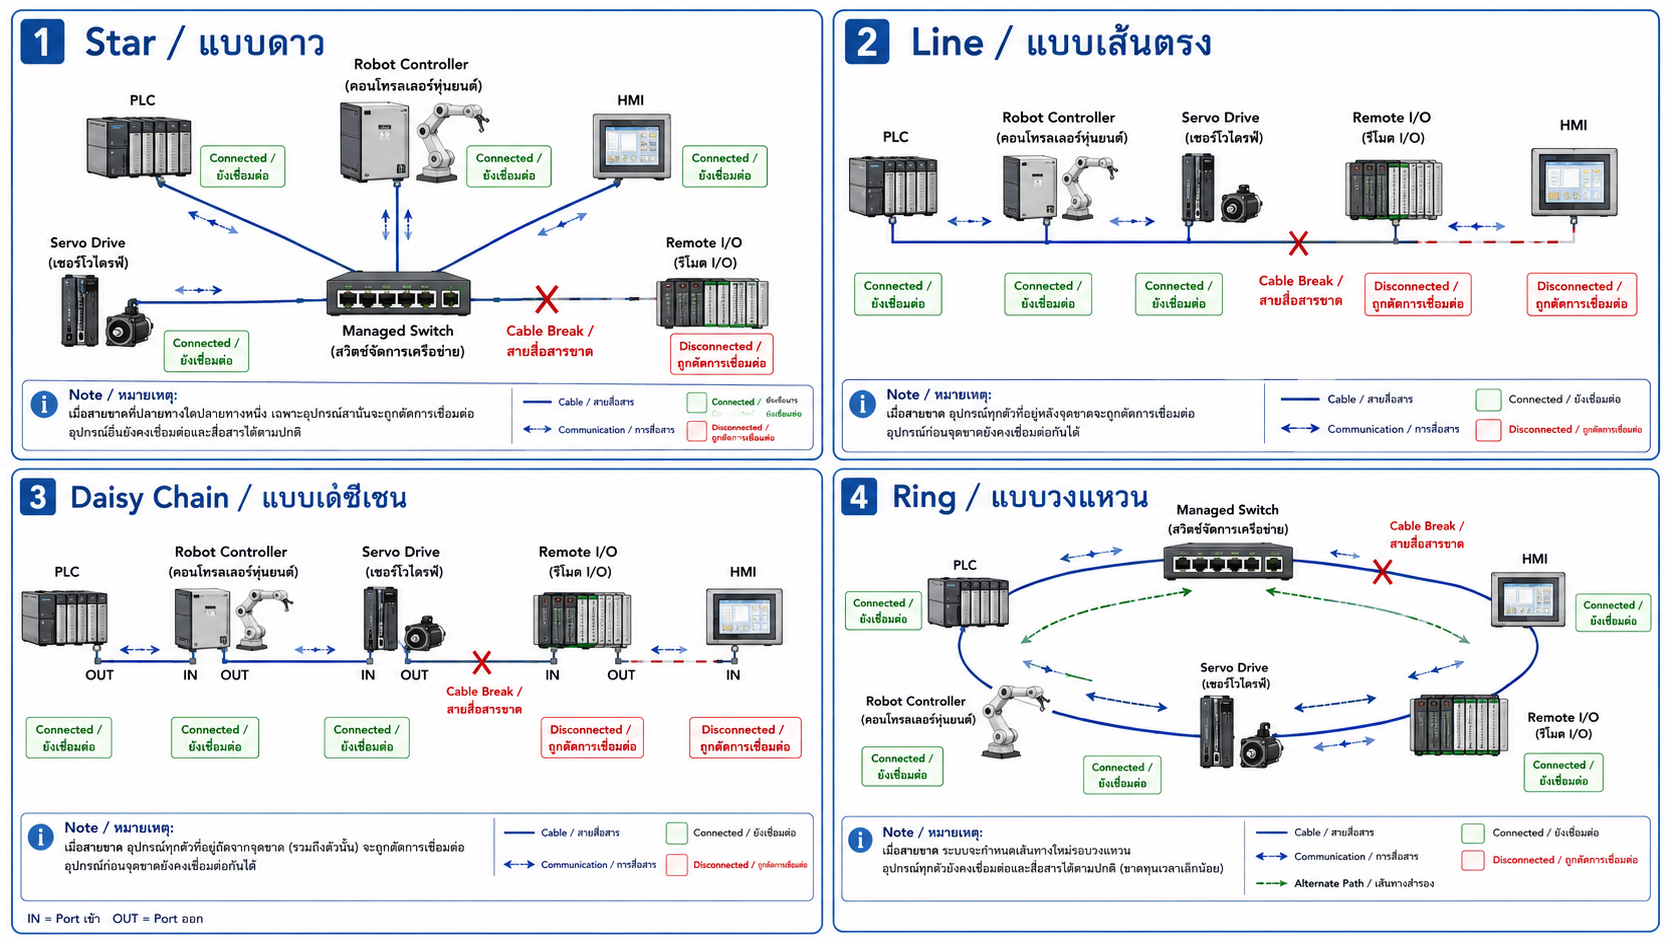
\includegraphics[width=0.8\textwidth]{images/chapter6/figure-06.png}
    \caption{โทโพโลยี Star, Line, Daisy Chain และ Ring}
\end{figure}



\subsubsection{การสื่อสารระดับสูง: OPC UA และ ROS-Industrial}

\paragraph{7.16.1 OPC UA}

OPC UA เป็นมาตรฐานที่ไม่ขึ้นกับแพลตฟอร์มสำหรับการแลกเปลี่ยนข้อมูลอย่างปลอดภัยและเชื่อถือได้ มี Information Model ที่ช่วยให้ข้อมูลมีความหมาย ไม่ใช่เพียง Address ตัวเลข จึงเหมาะกับ

\begin{itemize}
    \item Machine-to-Machine Integration
    \item เชื่อม Robot Cell กับ SCADA/MES
    \item Recipe และ Production Data
    \item Condition Monitoring
    \item Alarm และ Event
    \item Historical Data และ Digital Twin Integration
\end{itemize}

OPC UA มี Authentication, Encryption และ Integrity Mechanism แต่ต้อง Configuration Certificate, User Role และ Security Policy ให้ถูกต้อง การติดตั้งแบบเปิด Anonymous และไม่เข้ารหัสใน Production Network เพิ่มความเสี่ยง

\paragraph{7.16.2 ROS-Industrial}

ROS-Industrial ขยายความสามารถของ ROS ไปสู่งาน Manufacturing โดยมี Interface สำหรับ Industrial Manipulator, Gripper, Sensor และ Device Network รวมทั้งสนับสนุน Motion Planning, Calibration และ Perception

การใช้งานเหมาะกับงานที่ต้องการความยืดหยุ่นและ Algorithm ขั้นสูง แต่ควรแยกบทบาทจาก Safety PLC และ Servo Real-time Loop ไม่ควรถือว่า ROS Node ทั่วไปเป็น Safety-rated Controller โดยอัตโนมัติ



\subsubsection{Functional Safety กับระบบควบคุมและเครือข่าย}

Safety Function ในเซลล์หุ่นยนต์ต้องออกแบบจากการประเมินความเสี่ยงและอ้างอิงมาตรฐานที่เกี่ยวข้อง เช่น ISO 10218-1:2025 สำหรับ Industrial Robot, ISO 10218-2:2025 สำหรับ Robot Application/Cell และ IEC 60204-1 สำหรับอุปกรณ์ไฟฟ้าของเครื่องจักร

ตัวอย่าง Safety Function ได้แก่

\begin{itemize}
    \item Emergency Stop
    \item Protective Stop เมื่อประตูเปิด
    \item Safe Torque Off (STO)
    \item Safe Stop 1/2
    \item Safely Limited Speed
    \item Safe Position/Space Monitoring
    \item Enabling Device ใน Teaching Mode
\end{itemize}

\paragraph{7.17.1 Standard Control ไม่เท่ากับ Safety Control}

สัญญาณ Start, Running และ Program Select สามารถใช้ Standard I/O ได้ แต่ E-Stop และ Guard Interlock ต้องใช้ Safety-rated Architecture ตาม Performance Level หรือ SIL ที่กำหนดจาก Risk Assessment

\paragraph{7.17.2 Safety over Network}

โปรโตคอล เช่น PROFIsafe หรือ CIP Safety ส่ง Safety Data ผ่านเครือข่ายมาตรฐานด้วยกลไกตรวจสอบ เช่น Sequence, Time Expectation, Identifier และ CRC อย่างไรก็ตาม การใช้ชื่อ “Safety Protocol” ไม่เพียงพอ อุปกรณ์ทุกส่วน Configuration และ Validation ต้องรองรับระดับ Safety ที่ต้องการ

\paragraph{7.17.3 หลัก Fail-safe}

เมื่อเกิด Network Loss, Cable Break, Watchdog Timeout หรือข้อมูลไม่ถูกต้อง ระบบต้องเข้าสู่สถานะที่กำหนดไว้ล่วงหน้า โดยสถานะนั้นต้องลดความเสี่ยง ไม่ใช่เพียงหยุด Software Task



\subsubsection{การวินิจฉัยและการบำรุงรักษาเครือข่าย}

แนวทางวินิจฉัยจากชั้นล่างขึ้นชั้นบน

\begin{enumerate}
    \item \textbf{Physical:} Power, Connector, Cable, Shield, Ground, Link LED
    \item \textbf{Data Link:} MAC Error, Port Counter, Topology, Duplicate Device
    \item \textbf{Network:} IP Address, Subnet, Routing, Duplicate IP
    \item \textbf{Transport/Connection:} TCP State, UDP Loss, Connection Timeout
    \item \textbf{Application:} I/O Size, GSD/EDS/ESI, Tag Mapping, Function Code
    \item \textbf{Control Logic:} Handshake State, Interlock, Timeout, Sequence
\end{enumerate}

ข้อมูลที่ควรบันทึก

\begin{itemize}
    \item Network Diagram และ Port Map
    \item IP/Device Name Table
    \item Firmware และ Device Description Version
    \item I/O Mapping และ Data Type
    \item Cycle/Update Time
    \item Switch Configuration
    \item Baseline Error Counter
    \item Backup Configuration
\end{itemize}



\subsubsection{การเลือกโปรโตคอลให้เหมาะกับงาน}

ควรพิจารณาอย่างน้อย 8 ประเด็น

\begin{enumerate}
    \item Ecosystem ของ PLC และ Robot ที่มีอยู่
    \item Required Cycle Time และ Jitter
    \item จำนวน Axis และปริมาณ I/O
    \item ความต้องการ Motion Synchronization
    \item Diagnostics และ Predictive Maintenance
    \item Safety Communication
    \item Topology, Cable Length และสภาพแวดล้อม
    \item ทักษะบุคลากร อะไหล่ และต้นทุนตลอดอายุระบบ
\end{enumerate}

\paragraph{ตารางตัดสินใจเบื้องต้น}

\begin{table}[htbp]
    \centering
    \small
    \begin{tabularx}{\textwidth}{@{}X L{0.28\textwidth} X@{}}
        \hline
        \textbf{สถานการณ์} & \textbf{วิธีที่เหมาะสม} & \textbf{เหตุผล} \\
        \hline
        Robot เดี่ยว ต้องการ Start/Complete ไม่เกิน 20 สัญญาณ & Hard-wired I/O & เรียบง่าย วินิจฉัยง่าย ต้นทุนต่ำ \\
        ระบบเดิมมี Remote I/O จำนวนมากและใช้ Siemens & PROFIBUS DP หรือ PROFINET ตาม Controller & รักษาความเข้ากันได้และลดความเสี่ยง Migration \\
        PLC–Robot ต้องแลกสถานะและ Diagnostic จำนวนมาก & PROFINET หรือ EtherNet/IP & Cyclic I/O และ Acyclic Diagnostic \\
        Multi-axis Motion ต้อง Synchronize ต่ำกว่า 1 ms & EtherCAT, PROFINET IRT หรือ Real-time Ethernet ที่รองรับ & Timing และ Clock Synchronization ดีกว่าเครือข่าย Polling ทั่วไป \\
        ต้องเชื่อมข้อมูล Robot Cell กับ MES/Analytics & OPC UA ร่วมกับเครือข่ายควบคุม & Information Model และ Security Service \\
        งานวิจัย Vision/Motion Planning ขั้นสูง & ROS-Industrial ร่วมกับ Controller อุตสาหกรรม & Algorithm และ Interface ยืดหยุ่น แต่แยก Safety/Servo Loop \\
        \hline
    \end{tabularx}
\end{table}



\subsection{ความเข้าใจผิดที่พบบ่อย}

\subsubsection{Stepper Motor เป็นระบบวงเปิดจึงไม่มีวันคลาดเคลื่อน}

ไม่ถูกต้อง Stepper สามารถหลุด Step เมื่อโหลดสูง ความเร่งมาก หรือ Resonance เกิดขึ้น หากต้องการยืนยันตำแหน่งจริงต้องใช้ Encoder หรือเซนเซอร์อื่น

\subsubsection{\texorpdfstring{ “เพิ่ม $K_p$ ให้สูงที่สุดจะทำให้แม่นยำที่สุด”}{8.2 เพิ่ม Kp ให้สูงที่สุดจะทำให้แม่นยำที่สุด}}

$K_p$ สูงลด Error ได้ แต่เพิ่มโอกาส Overshoot, Oscillation, Noise Amplification และ Saturation ต้องพิจารณา Stability Margin และกลไกจริง

\subsubsection{“Integral Gain แก้ทุกปัญหา Error”}

Integral ช่วยกำจัด Error คงตัว แต่เพิ่ม Phase Lag และ Windup หากโหลดหรือคำสั่งเกินขีดจำกัด อาจทำให้ Recovery ช้าและ Overshoot สูง

\subsubsection{“Derivative Gain ทำให้ระบบเร็วขึ้นเสมอ”}

Derivative เพิ่ม Damping ในหลายกรณี แต่ไวต่อ Noise และการตั้งค่า Filter หากใช้ไม่เหมาะสมอาจสร้างคำสั่งกระชาก

\subsubsection{“Torque Control เท่ากับ Force Control ที่ปลายแขนโดยตรง”}

แรงบิดมอเตอร์ต้องผ่าน Gear Ratio, Efficiency, Friction, Jacobian และ Dynamics จึงจะแปลงเป็นแรงที่ปลายแขนได้

\subsubsection{“Ethernet 1 Gbps ต้องตอบสนองเร็วกว่า Fieldbus ทุกชนิด”}

Link Speed ไม่เท่ากับ Deterministic Response ต้องพิจารณา Scheduling, Stack, Switch, Load, Cycle และ Jitter

\subsubsection{“Cycle Time ที่ระบุในโบรชัวร์ใช้ได้กับทุกระบบ”}

ค่าดังกล่าวมักเป็นเงื่อนไขเฉพาะ จำนวน Node และ Payload จำกัด ต้องตรวจ Configuration จริงและ Worst-case

\subsubsection{“E-Stop ต่อเข้าขา PLC ปกติก็เพียงพอ”}

ไม่เพียงพอสำหรับ Safety Function โดยทั่วไป ต้องใช้ Safety-rated Architecture และ Validation ตาม Risk Assessment

\subsubsection{“OPC UA หรือ ROS แทน Servo Network ได้ทั้งหมด”}

OPC UA และ ROS-Industrial เหมาะกับการบูรณาการระดับข้อมูลและ Algorithm แต่ไม่แทน Hard Real-time Servo Loop หรือ Safety Function โดยอัตโนมัติ

\subsubsection{“หาก Ping ได้ แสดงว่าระบบ I/O ใช้งานได้”}

Ping ตรวจเพียง IP Connectivity บางส่วน ไม่ยืนยัน Device Name, I/O Module, Connection, Data Mapping หรือ Application State



\subsection{การประยุกต์ใช้ในงานจริง}

\subsubsection{เซลล์ Pick and Place กับสายพาน}

PLC รับ Photoelectric Sensor ตรวจชิ้นงาน ควบคุม Conveyor และส่ง Part Ready ไป Robot เมื่อ Robot พร้อมและพื้นที่ปลอดภัย PLC ส่ง Start Request Robot เคลื่อนด้วย Position Control และใช้ Vacuum Sensor ยืนยันการจับ หากจับไม่สำเร็จ Robot ส่ง Grip Fault ให้ PLC จัดการ Reject Sequence

\subsubsection{งาน Press-fit}

Robot เคลื่อนเข้าใกล้ด้วย Position Control จากนั้นเปลี่ยนเป็น Force/Torque Control หรือ Impedance Mode ใกล้ผิวสัมผัส ใช้ Force Sensor หรือ Motor Torque Estimate ตรวจแรงกด PLC บันทึก Peak Force และ Displacement ผ่าน Industrial Ethernet เพื่อประเมินคุณภาพ

\subsubsection{งานเชื่อมแบบหลายสถานี}

PLC ควบคุม Fixture, Fume Extraction และ Safety Interlock หุ่นยนต์รับ Program Number ตามรุ่นชิ้นงาน PROFINET หรือ EtherNet/IP ส่งสถานะ Welding, Arc Fault และ Cycle Complete ข้อมูล Production Count ส่งต่อ OPC UA ไป MES

\subsubsection{ระบบ Multi-axis Packaging}

Servo หลายแกนต้อง Synchronize กับ Conveyor Encoder จึงใช้ Real-time Ethernet ที่มี Distributed Clock หรือ Isochronous Mode วงรอบ Motion ทำงานระดับ Controller ส่วน PLC Sequence จัดการ Recipe และ Alarm

\subsubsection{Condition Monitoring}

Servo Drive ส่งข้อมูล Current, Torque, Temperature และ Following Error ผ่าน Acyclic Diagnostic ระบบวิเคราะห์แนวโน้มเพื่อระบุ Gear Wear, Bearing Friction หรือ Load Change โดยไม่แทรกแซงวงรอบควบคุมหลัก



\subsection{สรุปท้ายบท}

\begin{enumerate}
    \item ระบบวงเปิดไม่มี Feedback จึงง่ายและต้นทุนต่ำ แต่ไม่ชดเชยความคลาดเคลื่อนจากโหลดและ Disturbance โดยตรง
    \item ระบบวงปิดคำนวณ Error จากค่าตั้งและค่าที่วัด จึงเพิ่มความแม่นยำได้ แต่ต้องออกแบบเสถียรภาพ Bandwidth และ Noise Sensitivity
    \item PID ประกอบด้วยพจน์ P, I และ D ซึ่งมีบทบาทต่างกัน การปรับ Gain ต้องประเมิน Rise Time, Overshoot, Settling Time, Steady-state Error และ Control Effort
    \item Servo Axis มักใช้วงรอบซ้อน Current–Speed–Position โดยวงด้านในต้องเร็วกว่าและคงตัวก่อนวงด้านนอก
    \item Joint Space Control เหมาะกับการควบคุมตัวแปรข้อต่อ ส่วน Cartesian Space Control เหมาะกับเส้นทางและแรงที่ End Effector แต่ต้องใช้ Kinematics และ Jacobian
    \item Computed Torque Control ใช้แบบจำลอง Dynamics ชดเชย Inertia, Coriolis และ Gravity แต่ไวต่อ Model Error
    \item PLC และ Robot Controller ควรแลกคำสั่งด้วย Handshake, Interlock และ Timeout ไม่พึ่ง Pulse เดี่ยวโดยไม่มีการยืนยัน
    \item Standard I/O ต้องแยกจาก Safety-rated I/O โดยเฉพาะ E-Stop และ Guard Door
    \item การเลือก Fieldbus หรือ Industrial Ethernet ต้องพิจารณา Determinism, Cycle Time, Jitter, Diagnostics, Topology และ Ecosystem ไม่พิจารณา Link Speed เพียงอย่างเดียว
    \item PROFINET, EtherNet/IP, EtherCAT, Modbus TCP และ POWERLINK มีจุดเด่นต่างกัน ค่าประสิทธิภาพจริงขึ้นกับอุปกรณ์ Configuration และ Network Load
    \item OPC UA และ ROS-Industrial ช่วยบูรณาการระดับข้อมูลและ Algorithm แต่ไม่แทนวงรอบ Servo และ Functional Safety โดยอัตโนมัติ
    \item การวินิจฉัยควรเริ่มจาก Physical Layer ไปยัง Application และ Control Logic พร้อมเอกสาร Network Baseline ที่ครบถ้วน
\end{enumerate}



\subsection{คำถามทบทวนท้ายบท}

\begin{enumerate}
    \item อธิบายความแตกต่างระหว่าง Open-loop Control และ Closed-loop Control พร้อมยกตัวอย่างจากระบบหุ่นยนต์อย่างละหนึ่งตัวอย่าง
    \item เหตุใดการเพิ่ม $K_p$ มากเกินไปจึงอาจทำให้ระบบสั่น แม้ Steady-state Error จะลดลง
    \item Integral Windup เกิดขึ้นได้อย่างไร และมีแนวทางป้องกันอย่างไร
    \item เปรียบเทียบ Position, Speed และ Torque Control ในด้านตัวแปรป้อนกลับ งานที่เหมาะสม และข้อจำกัด
    \item เพราะเหตุใด Current Loop จึงต้องเร็วกว่าวงรอบ Speed และ Position
    \item Joint Space Control และ Cartesian Space Control แตกต่างกันอย่างไร และงานเชื่อมแนวเส้นตรงควรให้ความสำคัญกับวิธีใด
    \item อธิบายบทบาทของ Jacobian Matrix ในการควบคุมหุ่นยนต์
    \item เหตุใด PLC–Robot Interface จึงควรใช้ Handshake และ Timeout แทน Start Pulse เพียงสัญญาณเดียว
    \item เปรียบเทียบ Hard-wired I/O, Fieldbus และ Industrial Ethernet ในด้านปริมาณข้อมูล การวินิจฉัย และความซับซ้อน
    \item Modbus RTU และ Modbus TCP เหมือนและต่างกันอย่างไร
    \item เหตุใด EtherCAT จึงเหมาะกับงาน Multi-axis Motion มากกว่า Modbus TCP ในหลายกรณี
    \item Cycle Time, Latency และ Jitter แตกต่างกันอย่างไร
    \item Star, Line และ Ring Topology มีผลต่อความทนทานเมื่อสายขาดอย่างไร
    \item เหตุใด Emergency Stop จึงไม่ควรพึ่ง Standard PLC I/O เพียงอย่างเดียว
    \item OPC UA และ ROS-Industrial ควรอยู่ในระดับใดของสถาปัตยกรรม และเหตุใดจึงไม่ควรแทน Servo Loop โดยตรง
\end{enumerate}

\newpage

\subsection{กิจกรรมปฏิบัติการประจำบท}

\subsubsection{กิจกรรมปฏิบัติการที่ 6-1: การตั้งค่า PID และวิเคราะห์ Step Response ของ Servo Axis}

\paragraph{1. วัตถุประสงค์}

หลังปฏิบัติ นักศึกษาสามารถ

\begin{enumerate}
    \item ตั้งค่าการทดลอง Servo Axis ในโหมดที่ผู้ผลิตอนุญาตภายใต้ขีดจำกัดปลอดภัย
    \item ปรับค่า $K_p$, $K_i$ และ $K_d$ หรือค่าพารามิเตอร์เทียบเท่าของ Drive อย่างเป็นระบบ
    \item วัด Rise Time, Overshoot, Settling Time และ Steady-state Error
    \item วิเคราะห์ Trade-off ระหว่างความเร็ว ความแม่นยำ การสั่น และ Control Effort
    \item เลือกชุด Gain ที่เหมาะสมตามเกณฑ์ที่กำหนด
\end{enumerate}

\paragraph{2. หลักการและทฤษฎีที่เกี่ยวข้อง}

ใช้หลักการ PID ในหัวข้อ 7.4 และตัวชี้วัด Step Response ในหัวข้อ 7.3 การทดลองไม่มุ่งหาค่า Gain สูงสุด แต่หาค่าที่ทำให้ระบบผ่านเกณฑ์หลายด้านพร้อมกัน

ตัวชี้วัดหลัก

\[
M_p(\%)=\frac{y_{max}-y_{ss}}{y_{ss}}\times100
\]

และกำหนด Settling Time จากช่วงที่ผลตอบสนองอยู่ภายในแถบ $\pm2\%$ ของค่าปลายทาง หรือเกณฑ์ที่ผู้สอนกำหนด

\paragraph{3. อุปกรณ์ เครื่องมือ และซอฟต์แวร์}

\begin{enumerate}
    \item ชุดทดลอง Servo Drive และ Servo Motor แบบการศึกษา ชนิดติดตั้งสำเร็จ มี Guard ครอบเพลา จำนวน 1 ชุดต่อกลุ่ม
    \item แหล่งจ่ายและตู้ควบคุมที่ผู้ผลิตจัดให้ พร้อม Protective Earth
    \item Encoder ที่ติดมากับ Servo Motor
    \item โหลดปรับได้แบบมี Guard และค่าพิกัดไม่เกินคู่มือ
    \item Oscilloscope แบบ Isolated Input หรือ Data Acquisition ที่ผู้ผลิตอนุญาต
    \item คอมพิวเตอร์และซอฟต์แวร์ Commissioning ของ Servo Drive
    \item Emergency Stop และ Main Isolator ที่ผ่านการตรวจสอบก่อนเรียน
    \item แบบบันทึกผลและไฟล์ Configuration สำรอง
\end{enumerate}

\begin{quote}
หากไม่มี Servo Trainer จริง ให้ใช้ Digital Twin หรือ Simulator ของผู้ผลิตเพื่อศึกษาผลของ Gain โดยไม่สั่งมอเตอร์จริง
\end{quote}

\paragraph{4. แผนภาพชุดทดลอง}

\begin{verbatim}
PC Commissioning Software
          |
          v
Educational Servo Drive -- Current/Speed/Position Data --> Oscilloscope/Logger
          |
          v
Guarded Servo Motor -- Guarded Coupling -- Adjustable Educational Load
          ^
          | Encoder Feedback

Safety Chain: E-Stop -> Safety Relay/STO -> Servo Drive
\end{verbatim}

\paragraph{5. ข้อควรระวังด้านความปลอดภัย}

\begin{enumerate}
    \item ปฏิบัติภายใต้การกำกับของผู้สอนหรือผู้รับผิดชอบห้องปฏิบัติการ
    \item ใช้ชุดทดลองที่มี Guard ครอบเพลาและชิ้นส่วนหมุน ห้ามถอด Guard ขณะจ่ายพลังงาน
    \item ตรวจ E-Stop, STO และ Main Isolator ก่อนเริ่มทุกครั้ง
    \item ห้ามต่อ Probe เข้าวงจร Power Stage โดยตรง ใช้เฉพาะ Monitoring Port หรือ Isolated Measurement ที่ผู้ผลิตกำหนด
    \item จำกัด Speed, Torque, Travel และ Acceleration ให้อยู่ในค่าที่ผู้สอนกำหนด
    \item ห้ามปรับ Gain แบบก้าวกระโดดหรือปิด Protection Function
    \item หากได้ยินเสียงผิดปกติ เกิดการสั่นต่อเนื่อง หรือมี Alarm ให้กด Stop/E-Stop ตามขั้นตอนและแจ้งผู้สอน
    \item ห้ามจับเพลา Coupling หรือโหลดจนกว่าจะตัดพลังงานและยืนยันว่าไม่มีพลังงานสะสม
\end{enumerate}

\paragraph{6. ขั้นตอนการปฏิบัติ}

\textbf{ตอนที่ A ตรวจสอบระบบ}

\begin{enumerate}
    \item ตัดพลังงานและตรวจการต่อสายกับแผนภาพของผู้ผลิต
    \item ตรวจ Guard, Protective Earth และ Emergency Stop
    \item เปิดซอฟต์แวร์และบันทึกค่าพารามิเตอร์เดิมเป็น Backup
    \item กำหนด Current/Torque Limit, Speed Limit และ Acceleration Limit ตามใบงาน
    \item ทดสอบ Jog ที่ความเร็วต่ำเพื่อยืนยัน Encoder Direction และ Motor Direction
\end{enumerate}

\textbf{ตอนที่ B เก็บ Baseline}

\begin{enumerate}
    \item ใช้ค่า Gain มาตรฐานจากผู้ผลิตหรือค่าที่ผู้สอนจัดเตรียม
    \item สั่ง Step หรือ Speed Change ขนาดเล็กตามที่ชุดทดลองรองรับ
    \item บันทึก Command, Actual, Error และ Control Output
    \item ทำซ้ำอย่างน้อย 3 ครั้งและตรวจความสม่ำเสมอ
\end{enumerate}

\textbf{ตอนที่ C ปรับ $K_p$}

\begin{enumerate}
    \item กำหนด $K_i=0$ และ $K_d=0$ หาก Controller อนุญาตและผู้สอนกำหนด
    \item เพิ่ม $K_p$ ทีละขั้นขนาดเล็ก
    \item บันทึก Rise Time, Overshoot, Settling Time, Error และอาการสั่น
    \item หยุดเพิ่มเมื่อถึงขีดจำกัดที่ผู้สอนกำหนดหรือเริ่มเห็นแนวโน้มสั่น
\end{enumerate}

\textbf{ตอนที่ D ปรับ $K_i$}

\begin{enumerate}
    \item เลือก $K_p$ ที่ตอบสนองดีแต่ยังมี Margin
    \item เพิ่ม $K_i$ ทีละขั้นเพื่อแก้ Steady-state Error
    \item ทดสอบ Saturation ด้วยคำสั่งที่ยังอยู่ในขีดจำกัด และสังเกต Windup โดยไม่เกินค่าปลอดภัย
    \item เปิดใช้ Anti-windup หาก Drive รองรับ แล้วเปรียบเทียบ Recovery
\end{enumerate}

\textbf{ตอนที่ E ปรับ $K_d$ หรือ Damping Parameter}

\begin{enumerate}
    \item เพิ่มค่าอนุพันธ์หรือ Damping ทีละน้อย
    \item ตรวจ Noise ที่ Control Output และสังเกตผลของ Filter
    \item เลือกชุด Gain สุดท้ายตามเกณฑ์ เช่น Overshoot < 5\%, Settling Time < ค่าที่กำหนด และไม่มีการสั่นต่อเนื่อง
\end{enumerate}

\paragraph{7. ตารางบันทึกผล}

\begin{table}[htbp]
    \centering
    \resizebox{\textwidth}{!}{%
    \begin{tabular}{r r r r r r r r r l l}
        \hline
        \textbf{ชุดทดลอง} & \textbf{$K_p$} & \textbf{$K_i$} & \textbf{$K_d$} & \textbf{Rise Time (s)} & \textbf{Overshoot (\%)} & \textbf{Settling Time (s)} & \textbf{$e_{ss}$} & \textbf{Peak Output} & \textbf{อาการสั่น/Noise} & \textbf{ผ่านเกณฑ์} \\
        \hline
        Baseline &  &  &  &  &  &  &  &  &  &  \\
        P-1 &  & 0 & 0 &  &  &  &  &  &  &  \\
        P-2 &  & 0 & 0 &  &  &  &  &  &  &  \\
        PI-1 &  &  & 0 &  &  &  &  &  &  &  \\
        PID-1 &  &  &  &  &  &  &  &  &  &  \\
        Final &  &  &  &  &  &  &  &  &  &  \\
        \hline
    \end{tabular}
    }
\end{table}

\paragraph{8. การคำนวณและวิเคราะห์ผล}

\begin{enumerate}
    \item คำนวณ Overshoot จากข้อมูลที่วัด
    \item ระบุเกณฑ์ Rise Time และ Settling Band ที่ใช้
    \item สร้างกราฟเปรียบเทียบอย่างน้อย 3 ชุด Gain
    \item วิเคราะห์ว่าการเพิ่ม Gain แต่ละพจน์เปลี่ยน Control Effort อย่างไร
    \item ตรวจว่าชุด Gain ที่เร็วที่สุดเป็นชุดที่เหมาะสมที่สุดหรือไม่
    \item อภิปรายความแตกต่างระหว่างผลจริงกับแนวโน้มในตารางทฤษฎี
\end{enumerate}

\paragraph{9. การเปรียบเทียบผลจริงกับทฤษฎี}

ผลจริงอาจไม่ตรงแนวโน้มทั่วไปเนื่องจาก

\begin{itemize}
    \item Drive ใช้ PID Form หรือ Gain Scaling ต่างจากสมการมาตรฐาน
    \item มี Feedforward, Filter, Notch Filter หรือ Auto-tuning ทำงานอยู่
    \item Plant มี Backlash, Friction และ Resonance
    \item Sampling Time และ Data Logging Rate จำกัด
    \item Output Saturation และ Anti-windup เปลี่ยนพฤติกรรม
\end{itemize}

\paragraph{10. คำถามหลังการทดลอง}

\begin{enumerate}
    \item ชุด Gain ใดให้ Rise Time ต่ำที่สุด และมีข้อเสียใด
    \item $K_i$ ช่วยลด Error ได้จริงหรือไม่ และทำให้ Overshoot เปลี่ยนอย่างไร
    \item เมื่อเกิด Saturation ระบบใช้เวลาฟื้นตัวเท่าใดก่อนและหลัง Anti-windup
    \item $K_d$ หรือ Damping Parameter เพิ่ม Noise หรือไม่
    \item หากเพิ่มโหลด ผลตอบสนองและค่า Gain ที่เหมาะสมเปลี่ยนอย่างไร
\end{enumerate}

\paragraph{11. เกณฑ์การประเมิน}

\begin{table}[htbp]
    \centering
    \begin{tabular}{l r}
        \hline
        \textbf{ด้านที่ประเมิน} & \textbf{คะแนน} \\
        \hline
        ตรวจสอบความปลอดภัยและปฏิบัติตามขั้นตอน & 20 \\
        การตั้งค่าและเก็บข้อมูลถูกต้อง & 20 \\
        การคำนวณตัวชี้วัด & 20 \\
        การวิเคราะห์ Trade-off และเลือก Gain & 25 \\
        รายงาน กราฟ และการอภิปราย & 15 \\
        \textbf{รวม} & \textbf{100} \\
        \hline
    \end{tabular}
\end{table}



\subsubsection{กิจกรรมปฏิบัติการที่ 6-2: การเชื่อมต่อ PLC กับ Robot Controller ผ่าน Hard-wired I/O}

\paragraph{1. วัตถุประสงค์}

หลังปฏิบัติ นักศึกษาสามารถ

\begin{enumerate}
    \item จัดทำ I/O List และ Wiring Diagram สำหรับ PLC–Robot Interface
    \item ต่อ Standard 24 VDC I/O เมื่อระบบถูกตัดพลังงานและตรวจสอบแล้ว
    \item เขียน Ladder Logic สำหรับ Handshake, Interlock และ Timeout
    \item ทดสอบ Start, Running, Complete, Fault และ Reset Sequence
    \item อธิบายการแยก Standard Control จาก Safety Circuit ได้
\end{enumerate}

\paragraph{2. หลักการและทฤษฎีที่เกี่ยวข้อง}

ใช้แนวคิด Digital I/O, PNP/NPN, Handshake, Program Select และ Timeout ในหัวข้อ 7.8 โดยกำหนด State Machine อย่างน้อย 5 สถานะ

\begin{verbatim}
IDLE -> REQUEST -> ACKNOWLEDGED -> RUNNING -> COMPLETE -> IDLE
                      +------------ FAULT ------------+
\end{verbatim}

\paragraph{3. อุปกรณ์ เครื่องมือ และซอฟต์แวร์}

\begin{enumerate}
    \item PLC Trainer 24 VDC จำนวน 1 ชุด
    \item Robot Controller Simulator หรือ Educational Robot Cell ที่มี Standard I/O Interface
    \item Interface Relay/Optocoupler Module ตามชนิด I/O
    \item Terminal Block, Fuse และสาย Patch สำหรับการศึกษา
    \item Multimeter CAT-rated ที่เหมาะสมกับ 24 VDC
    \item คอมพิวเตอร์และ PLC Programming Software
    \item Safety Relay/Guard Circuit ที่ \textbf{ติดตั้งและตรวจสอบล่วงหน้าโดยผู้สอน}
    \item Emergency Stop และ Guard ที่เป็นส่วนหนึ่งของชุดฝึก
\end{enumerate}

\paragraph{4. แผนภาพหรือวงจร}

Standard I/O ที่ใช้ในการทดลอง

\begin{table}[htbp]
    \centering
    \begin{tabular}{l l l}
        \hline
        \textbf{PLC Output \(\to\) Robot Input} & \textbf{PLC Address} & \textbf{Robot Signal} \\
        \hline
        Start\_Request & Q0.0 & DI\_START\_REQ \\
        Reset\_Request & Q0.1 & DI\_RESET\_REQ \\
        Program\_Bit0 & Q0.2 & DI\_PROG\_0 \\
        Program\_Bit1 & Q0.3 & DI\_PROG\_1 \\
        Program\_Bit2 & Q0.4 & DI\_PROG\_2 \\
        Program\_Bit3 & Q0.5 & DI\_PROG\_3 \\
        \hline
    \end{tabular}
\end{table}

\begin{table}[htbp]
    \centering
    \begin{tabular}{l l l}
        \hline
        \textbf{Robot Output \(\to\) PLC Input} & \textbf{Robot Signal} & \textbf{PLC Address} \\
        \hline
        Ready & DO\_READY & I0.0 \\
        Start\_Ack & DO\_START\_ACK & I0.1 \\
        Running & DO\_RUNNING & I0.2 \\
        Complete & DO\_COMPLETE & I0.3 \\
        Fault & DO\_FAULT & I0.4 \\
        Home & DO\_HOME & I0.5 \\
        \hline
    \end{tabular}
\end{table}

\paragraph{5. ข้อควรระวังด้านความปลอดภัย}

\begin{enumerate}
    \item การต่อสายทำเฉพาะวงจร 24 VDC Standard I/O และต้องตัดพลังงานก่อนทุกครั้ง
    \item Safety Circuit ต้องติดตั้งล่วงหน้าโดยผู้มีอำนาจและห้ามนักศึกษาดัดแปลง
    \item E-Stop ใช้ Safety Relay/Safety PLC ไปยัง Robot Safety Interface ไม่ผ่าน Standard PLC Output
    \item ทดสอบ Logic ใน Simulator ก่อนอนุญาต Motion จริง
    \item หากใช้ Robot จริง ให้จำกัดความเร็วและพื้นที่ พร้อมผู้สอนควบคุม Pendant
    \item ตรวจ PNP/NPN และ Common 0 V ก่อนจ่ายไฟ
    \item ใช้ Fuse แยก Branch และห้าม Short Terminal เพื่อจำลอง Fault
    \item การจำลอง Fault ใช้ Software Flag หรือ Disconnect Plug ที่ออกแบบสำหรับ Trainer เท่านั้น
\end{enumerate}

\paragraph{6. ขั้นตอนการปฏิบัติ}

\textbf{ตอนที่ A ออกแบบ}

\begin{enumerate}
    \item จัดทำ I/O List และกำหนดทิศทางสัญญาณ
    \item วาด Wiring Diagram แยก Standard I/O กับ Safety Circuit
    \item กำหนด State Machine และ Timeout ของแต่ละขั้น
    \item ตรวจแบบร่วมกับผู้สอน
\end{enumerate}

\textbf{ตอนที่ B ต่อวงจร Standard I/O}

\begin{enumerate}
    \item ตัดพลังงานและ Lock/Tag ตามขั้นตอนห้องปฏิบัติการ
    \item ต่อ PLC Output ผ่าน Interface Module ไป Robot Input
    \item ต่อ Robot Output กลับ PLC Input
    \item ตรวจ Continuity และขั้ว Common
    \item ให้ผู้สอนตรวจและอนุญาตก่อนจ่าย 24 VDC
\end{enumerate}

\textbf{ตอนที่ C เขียน Ladder Logic}

\begin{enumerate}
    \item สร้าง Permissive: Ready AND Home AND No Fault AND Cell Safe Status
    \item Latch Cycle Request เมื่อกด Start และ Permissive ครบ
    \item ส่ง Start\_Request จนได้รับ Start\_Ack
    \item เริ่ม Timer หาก Ack ไม่มาภายในเวลาที่กำหนด
    \item เมื่อ Running เป็น 1 ให้เข้าสถานะ RUNNING
    \item เมื่อ Complete เป็น 1 ให้บันทึก Cycle Complete และ Reset Request ตาม Handshake
    \item เมื่อ Fault เป็น 1 ให้ยกเลิกคำสั่ง Start และเข้าสถานะ FAULT
\end{enumerate}

\textbf{ตอนที่ D ทดสอบ}

\begin{enumerate}
    \item ทดสอบ Normal Cycle อย่างน้อย 3 รอบ
    \item ทดสอบ Robot Not Ready
    \item ทดสอบ Start\_Ack Timeout ผ่าน Simulator
    \item ทดสอบ Fault ระหว่าง Running
    \item ทดสอบการคืนระบบหลัง Reset ตามคู่มือ
    \item ให้ผู้สอนสาธิตการทำงานของ Safety Circuit แยกจาก Standard Logic โดยไม่ให้นักศึกษาปรับแก้
\end{enumerate}

\paragraph{7. ตารางบันทึกผล}

\begin{table}[htbp]
    \centering
    \resizebox{\textwidth}{!}{%
    \begin{tabular}{l r r r r r r r r l l}
        \hline
        \textbf{Test Case} & \textbf{Ready} & \textbf{Home} & \textbf{Fault} & \textbf{Start Req} & \textbf{Start Ack} & \textbf{Running} & \textbf{Complete} & \textbf{Timeout} & \textbf{ผลที่คาดหวัง} & \textbf{ผลที่สังเกต} \\
        \hline
        Normal cycle & 1 & 1 & 0 & 1 & 1 & 1 & 1 & 0 & จบรอบปกติ &  \\
        Not ready & 0 & 1 & 0 & 0 & 0 & 0 & 0 & 0 & ไม่ส่ง Start &  \\
        Ack timeout & 1 & 1 & 0 & 1 & 0 & 0 & 0 & 1 & เข้าสถานะ Fault &  \\
        Fault during run & 1 & 1 & 1 & 0 & - & 0 & 0 & - & ยกเลิก Sequence &  \\
        Reset recovery & 1 & 1 & 0 & 0 & 0 & 0 & 0 & 0 & กลับ IDLE &  \\
        \hline
    \end{tabular}
    }
\end{table}

\paragraph{8. การคำนวณและวิเคราะห์ผล}

\begin{enumerate}
    \item วัดเวลาจาก Start\_Request ถึง Running
    \item วัดเวลาจาก Complete ถึง PLC รับรู้
    \item เปรียบเทียบกับ PLC Scan และ Input Filter
    \item ประเมิน Timeout ที่เหมาะสมโดยมี Margin
    \item ตรวจว่าคำสั่ง Start ถูกยกเลิกเมื่อ Fault หรือ Permissive หายหรือไม่
\end{enumerate}

\paragraph{9. การเปรียบเทียบผลจริงกับทฤษฎี}

ความล่าช้าอาจเกิดจาก Input Filter, PLC Scan, Relay Delay, Robot Task และ Debounce การใช้ Relay เพิ่ม Isolation แต่เพิ่ม Delay และจุดสึกหรอ จึงควรเลือกตามความต้องการและจำนวนรอบ

\paragraph{10. คำถามหลังการทดลอง}

\begin{enumerate}
    \item หาก Start\_Request เป็น Pulse สั้นกว่า PLC/Robot Scan จะเกิดปัญหาใด
    \item เหตุใด Start\_Ack ต้องตอบกลับก่อน PLC ปิด Request
    \item Timeout สั้นและยาวเกินไปมีผลอย่างไร
    \item ถ้า Robot Fault ระหว่าง Running PLC ควรเก็บสถานะใดไว้เพื่อวินิจฉัย
    \item Safety Circuit แตกต่างจาก Standard Interlock ในด้านใด
\end{enumerate}

\paragraph{11. เกณฑ์การประเมิน}

\begin{table}[htbp]
    \centering
    \begin{tabular}{l r}
        \hline
        \textbf{ด้านที่ประเมิน} & \textbf{คะแนน} \\
        \hline
        I/O List และ Wiring Diagram & 20 \\
        การต่อวงจร 24 VDC อย่างปลอดภัย & 20 \\
        Ladder Handshake และ Timeout & 25 \\
        การทดสอบกรณีปกติและ Fault & 20 \\
        การวิเคราะห์และรายงาน & 15 \\
        \textbf{รวม} & \textbf{100} \\
        \hline
    \end{tabular}
\end{table}

\newpage

\subsection{แบบฝึกหัดท้ายบท}

\subsubsection{ระดับพื้นฐาน}

\textbf{ข้อ 1} \\
อธิบายความหมายของ Setpoint, Actual Value และ Error ในระบบควบคุมตำแหน่งของข้อต่อหุ่นยนต์

\textbf{ข้อ 2} \\
ระบุข้อดีสองข้อและข้อจำกัดสองข้อของระบบควบคุมวงเปิด

\textbf{ข้อ 3} \\
ตัวควบคุม PID มี $K_p=3$, $K_i=0.5\ \text{s}^{-1}$ และ $K_d=0.2\ \text{s}$ ณ ขณะหนึ่ง $e=0.4$, $\int e\,dt=0.6$ และ $de/dt=-0.5$ จงคำนวณ $u$

\textbf{ข้อ 4} \\
ระบบตำแหน่งได้รับคำสั่ง $50^\circ$ และมีค่าสูงสุด $57^\circ$ ก่อนคงตัวที่ $50^\circ$ จงคำนวณ Overshoot เป็นร้อยละ

\textbf{ข้อ 5} \\
เปรียบเทียบข้อมูล Cyclic และ Acyclic พร้อมยกตัวอย่างอย่างละสองรายการใน Robot–PLC Network

\subsubsection{ระดับวิเคราะห์}

\textbf{ข้อ 6} \\
ระบบ Servo มี Current Loop Bandwidth 1500 Hz หากใช้อัตราส่วนเริ่มต้น 5:1 ระหว่างวงรอบ จงประมาณ Speed Loop และ Position Loop Bandwidth พร้อมอธิบายเหตุผลที่ต้องแยก Bandwidth

\textbf{ข้อ 7} \\
ระบบ Joint Position Control มี Plant Gain $G=1.2$ และใช้ Proportional Controller $K_p=5$ กับ Unity Feedback จงหา Closed-loop Static Gain และ Steady-state Error เมื่อสั่ง Step ขนาด 1 หน่วย

\textbf{ข้อ 8} \\
Torque Sensor ช่วง 4–20 mA แทนแรงบิด $-100$ ถึง $300\ \text{N·m}$ หากวัดได้ 10 mA จงคำนวณแรงบิด

\textbf{ข้อ 9} \\
PLC Scan 10 ms, Input Filter 3 ms, Network Update ไปและกลับด้านละ 2 ms, Robot Processing 15 ms และ Output Delay 4 ms จงประมาณเวลาตอบสนองรวม พร้อมเสนอ Timeout ขั้นต่ำที่สมเหตุสมผลสำหรับ Handshake ที่ไม่ใช่ Safety

\textbf{ข้อ 10} \\
โรงงานมี Robot 1 ตัว ต้องการเพียง Start, Reset, Ready, Running, Complete, Fault และ Program Select 4 บิต ระยะสาย 15 m ไม่มีความต้องการ Diagnostic จำนวนมาก จงเปรียบเทียบ Hard-wired I/O กับ Industrial Ethernet และเสนอวิธีที่เหมาะสม

\subsubsection{13.3 ระดับประยุกต์ใช้}

\textbf{ข้อ 11} \\
ออกแบบ I/O Handshake สำหรับเซลล์ Pick and Place ที่มี PLC, Robot, Conveyor และ Gripper โดยระบุอย่างน้อย 6 สัญญาณจาก PLC ไป Robot, 6 สัญญาณจาก Robot ไป PLC, ลำดับ Normal Cycle และ Timeout/Fault Handling

\textbf{ข้อ 12} \\
สายการผลิตต้องควบคุม Servo 12 แกนให้ Synchronize ด้วย Cycle Time ต่ำกว่า 1 ms พร้อมอ่าน Remote I/O และส่งข้อมูล Production ไป MES จงเสนอ Architecture ที่แยก Motion Network, PLC/Cell Network และ Information Network พร้อมเหตุผล

\textbf{ข้อ 13} \\
ระหว่างทดสอบ PROFINET ระหว่าง S7-1500 กับ Robot พบว่า Link LED ติดและ Ping ได้ แต่ PLC แสดง Device Not Reachable และไม่มี I/O Data จงสร้างลำดับวินิจฉัยอย่างน้อย 8 ขั้นตอน โดยเริ่มจาก Physical/Identification ไปยัง Configuration และ Application Mapping

\newpage

\subsection{แนวคำตอบแบบฝึกหัดสำหรับผู้สอน}

\subsubsection{14.1 ระดับพื้นฐาน}

\textbf{แนวคำตอบข้อ 1} \\
Setpoint คือตำแหน่งที่ต้องการ เช่น $30^\circ$; Actual Value คือตำแหน่งที่ Encoder วัดได้; Error คือผลต่าง $e=q_d-q$ หาก Setpoint $30^\circ$ และวัดได้ $28^\circ$ จะมี Error $2^\circ$

\textbf{แนวคำตอบข้อ 2} \\
ข้อดี เช่น โครงสร้างง่าย ต้นทุนต่ำ และไม่ต้องใช้เซนเซอร์บางกรณี ข้อจำกัด เช่น ไม่ทราบความคลาดเคลื่อนจริงและไม่ชดเชยโหลดเปลี่ยนโดยตรง

\textbf{แนวคำตอบข้อ 3}

\[
u=K_pe+K_i\int e\,dt+K_d\frac{de}{dt}
\]

\[
u=3(0.4)+0.5(0.6)+0.2(-0.5)
\]

\[
u=1.2+0.3-0.1=1.4
\]

ดังนั้น $u=1.4$ หน่วยคำสั่ง

\textbf{แนวคำตอบข้อ 4}

\[
M_p=\frac{57-50}{50}\times100=14\%
\]

\textbf{แนวคำตอบข้อ 5} \\
Cyclic Data ส่งเป็นรอบ เช่น Ready, Running, Actual Position และ I/O Process Data ส่วน Acyclic Data ส่งเมื่อร้องขอ เช่น Parameter, Device Identification, Alarm History และ Diagnostic Record

\subsubsection{14.2 ระดับวิเคราะห์}

\textbf{แนวคำตอบข้อ 6}

\[
f_v=\frac{1500}{5}=300\ \text{Hz}
\]

\[
f_p=\frac{300}{5}=60\ \text{Hz}
\]

ต้องแยก Bandwidth เพื่อให้วงด้านในเข้าสู่สภาวะตอบสนองก่อนวงด้านนอก ลดการรบกวนกันและทำให้การออกแบบแต่ละวงง่ายขึ้น ค่าจริงต้องยืนยันกับ Plant

\textbf{แนวคำตอบข้อ 7}

\[
T=\frac{K_pG}{1+K_pG}=\frac{5(1.2)}{1+5(1.2)}=\frac{6}{7}=0.8571
\]

สำหรับ Step ขนาด 1

\[
e_{ss}=1-0.8571=0.1429
\]

หรือประมาณ 14.29\%

\textbf{แนวคำตอบข้อ 8}

\[
\tau=-100+\frac{10-4}{16}[300-(-100)]
\]

\[
\tau=-100+\frac{6}{16}(400)=-100+150=50\ \text{N·m}
\]

\textbf{แนวคำตอบข้อ 9}

\[
T=3+10+2+15+2+4=36\ \text{ms}
\]

Timeout ต้องมากกว่า Worst-case 36 ms และเผื่อ Jitter/Scan Alignment ตัวอย่างค่าที่สมเหตุสมผลคือ 100 ms หรือ 150 ms สำหรับ Handshake ทั่วไป ทั้งนี้ต้องทดสอบจริงและไม่ใช้เป็น Safety Response Time

\textbf{แนวคำตอบข้อ 10} \\
Hard-wired I/O ใช้สัญญาณประมาณ 10–14 จุด โครงสร้างง่าย ระยะ 15 m จัดการได้และวินิจฉัยด้วยไฟสถานะง่าย Industrial Ethernet ลดสายและขยายข้อมูลได้ แต่เพิ่ม Configuration, Switch และทักษะ หากไม่มีแผนขยายหรือ Diagnostic มาก Hard-wired I/O เหมาะสมกว่า โดยต้องแยก Safety Circuit ออกจาก Standard I/O

\subsubsection{14.3 ระดับประยุกต์ใช้}

\textbf{แนวคำตอบข้อ 11}

\begin{itemize}
    \item \textbf{PLC \(\to\) Robot:} Start\_Request, Reset\_Request, Part\_Present, Conveyor\_Stopped, Fixture\_Ready, Program\_Select และ Grip\_Enable
    \item \textbf{Robot \(\to\) PLC:} Ready, Start\_Ack, Running, At\_Pick, Grip\_OK, Complete, Fault และ Home
\end{itemize}

ลำดับ: PLC ตรวจ Permissive \(\to\) ส่ง Program/Start \(\to\) Robot Ack \(\to\) PLC ปิด Request \(\to\) Robot Running \(\to\) จับชิ้นงานและยืนยัน Grip \(\to\) วางชิ้นงาน \(\to\) Complete \(\to\) PLC Ack Complete \(\to\) กลับ Idle \\
กำหนด Timeout สำหรับ Ack, Grip และ Complete หาก Timeout ให้หยุด Sequence เก็บ Fault Code และรอ Recovery ที่กำหนด

\textbf{แนวคำตอบข้อ 12} \\
ใช้ Motion Network แบบ EtherCAT, PROFINET IRT หรือ Real-time Ethernet ที่รองรับ Cycle ต่ำกว่า 1 ms สำหรับ 12 Servo Axis; ใช้ PLC/Cell Network เช่น PROFINET RT หรือ EtherNet/IP สำหรับ Robot, Remote I/O และ HMI; ใช้ OPC UA ผ่าน Industrial DMZ/Information Layer ส่ง Production Data ไป MES แยก Traffic และ Security Zone เพื่อไม่ให้ MES Traffic รบกวน Motion

\textbf{แนวคำตอบข้อ 13}

\begin{enumerate}
    \item ตรวจสาย Connector และ Link Speed
    \item ตรวจ Switch Port/VLAN
    \item ตรวจ PROFINET Device Name
    \item ตรวจ IP/Subnet และ Duplicate IP
    \item ตรวจว่า PLC Project ใช้ GSDML ถูก Version
    \item ตรวจ Device/Slot/Subslot และขนาด I/O Module
    \item ตรวจ Update Time และ Watchdog
    \item ตรวจ Robot Option Package และ WorkVisual Configuration
    \item ตรวจ I/O Mapping/Byte Offset/Bit Order
    \item อ่าน PLC Diagnostic Buffer และ Robot Log
    \item Download Configuration ใหม่และ Power Cycle ตามคู่มือ
    \item ทดสอบด้วย I/O Pattern ง่ายก่อนเพิ่ม Handshake
\end{enumerate}



\subsection{ข้อเสนอแนะสำหรับผู้สอน}

\subsubsection{ลำดับการสอนที่แนะนำ}

\begin{enumerate}
    \item เริ่มจากสถานการณ์ Stepper หลุด Step และ Servo รักษาตำแหน่งเพื่อสร้างความแตกต่างวงเปิด–วงปิด
    \item ใช้ Block Diagram ก่อนสมการ แล้วจึงสร้างฟังก์ชันถ่ายโอนวงปิด
    \item อธิบาย PID จากความหมายทางกายภาพ ไม่เริ่มด้วยสูตรเพียงอย่างเดียว
    \item สาธิต Step Response และให้ผู้เรียนระบุ Rise Time, Overshoot และ Settling Time
    \item เชื่อม PID ไปยัง Cascade Loop ของ Servo Drive
    \item อธิบาย Joint/Cartesian ด้วยตัวอย่าง PTP กับ Linear Welding Path
    \item ใช้ I/O List จริงให้ผู้เรียนออกแบบ Handshake ก่อนต่อวงจร
    \item เปรียบเทียบ Protocol ด้วย Requirement Table ไม่ใช้การท่องจำความเร็วอย่างเดียว
    \item ปิดท้ายด้วย Safety Separation และกรณีวินิจฉัยเครือข่าย
\end{enumerate}

\subsubsection{จุดที่ผู้เรียนมักมีปัญหา}

\begin{itemize}
    \item สับสนระหว่าง Error กับ Output
    \item คิดว่า Gain สูงหมายถึงดีเสมอ
    \item ไม่แยก Link Speed, Cycle Time และ Latency
    \item สับสนว่า Modbus RTU และ Modbus TCP เป็น Physical Layer เดียวกัน
    \item มองข้าม Byte Order และ Data Type
    \item ใช้ Start Pulse โดยไม่มี Acknowledge
    \item รวม Safety Signal กับ Standard I/O ใน Logic เดียวโดยไม่เข้าใจระดับ Safety
\end{itemize}

\subsubsection{วิธีปรับระดับกิจกรรม}

\textbf{สำหรับผู้เรียนพื้นฐานอ่อน}

\begin{itemize}
    \item ใช้กราฟเชิงคุณภาพก่อนคำนวณ
    \item ให้ I/O Mapping Template สำเร็จบางส่วน
    \item จำกัดการทดลอง PID เป็น P และ PI
    \item ใช้ Simulator แทน Servo จริง
\end{itemize}

\textbf{สำหรับผู้เรียนพื้นฐานดี}

\begin{itemize}
    \item เพิ่มการวิเคราะห์ Sensitivity และ Phase Margin
    \item เปรียบเทียบ PID Form ของ Drive สองยี่ห้อ
    \item ออกแบบ State Machine ด้วย Sequential Function Chart
    \item วิเคราะห์ Network Load และ Worst-case Response
    \item เพิ่มกรณี Safety over Network และ Validation Plan
\end{itemize}

\subsubsection{การประเมินระหว่างเรียน}

\begin{itemize}
    \item Exit Ticket: อธิบายว่าทำไม $K_i$ จึงกำจัด Error แต่เพิ่มความเสี่ยง Overshoot
    \item Diagram Check: ให้เติม Feedback Path และ Disturbance ใน Block Diagram
    \item Protocol Card Sort: จัดกลุ่ม Serial Fieldbus, Industrial Ethernet และ Information Layer
    \item Fault Diagnosis: ให้ Log/LED สมมติและเรียงขั้นตอนตรวจสอบ
    \item I/O Review: ตรวจว่ามี Ack, Timeout และ Fault Reset ครบหรือไม่
\end{itemize}

\subsubsection{สัดส่วนการประเมินที่แนะนำ}

\begin{table}[htbp]
    \centering
    \begin{tabular}{l r}
        \hline
        \textbf{รายการ} & \textbf{สัดส่วน} \\
        \hline
        คำถามทบทวนและ Quiz & 15\% \\
        แบบฝึกหัดคำนวณและวิเคราะห์ & 20\% \\
        ใบงาน 6-1 PID & 25\% \\
        ใบงาน 6-2 PLC–Robot I/O & 25\% \\
        กรณีศึกษาเลือก Network & 15\% \\
        \textbf{รวม} & \textbf{100\%} \\
        \hline
    \end{tabular}
\end{table}



\subsection{สื่อและแหล่งเรียนรู้เพิ่มเติม}

\begin{table}[htbp]
    \centering
    \small
    \begin{tabularx}{\textwidth}{@{}L{0.20\textwidth} X X X L{0.12\textwidth}@{}}
        \hline
        \textbf{องค์กร/ผู้จัดทำ} & \textbf{หัวข้อที่ควรค้น} & \textbf{คำค้นแนะนำ} & \textbf{จุดประสงค์} & \textbf{ช่วงเวลาที่เหมาะสม} \\
        \hline
        Siemens / PROFIBUS \& PROFINET International & PROFINET Basics, RT/IRT, Diagnostics & “PROFINET system description”, “PROFINET RT IRT” & เข้าใจ Device, Controller, Update Time และ Topology & หลังหัวข้อ 7.13 \\
        ODVA & EtherNet/IP, CIP, RPI, DLR & “ODVA EtherNet/IP technology”, “CIP network” & เปรียบเทียบ CIP Messaging และ Infrastructure & หลังหัวข้อ 7.13 \\
        EtherCAT Technology Group & EtherCAT Principle และ Distributed Clocks & “EtherCAT technology processing on the fly” & เข้าใจเหตุผลของ Cycle Time ต่ำ & หลังหัวข้อ 7.13 \\
        Modbus Organization & Modbus Application Protocol และ Serial Guide & “Modbus application protocol specification” & แยก Application Protocol จาก RS-485/TCP & หลังหัวข้อ 7.12 \\
        CAN in Automation & CANopen และ CiA 402 & “CANopen CiA 402 drives motion control” & ศึกษา Object Dictionary และ Drive State Machine & หลังหัวข้อ 7.12 \\
        OPC Foundation & OPC UA Overview, Security และ Information Model & “OPC UA overview concepts security” & เชื่อมข้อมูลระดับเครื่องกับ Enterprise & หลังหัวข้อ 7.16 \\
        ROS-Industrial Consortium & Industrial Robot Interfaces และ Tutorials & “ROS-Industrial training motion planning” & ศึกษาการเชื่อม Algorithm ขั้นสูงกับหุ่นยนต์ & หลังหัวข้อ 7.16 \\
        KUKA & KUKA.PROFINET M/S และ System Software & “KUKA PROFINET M/S robot controller” & ดูตัวอย่าง Integration ของ Robot กับ PLC & ก่อนใบงาน 6-2 \\
        \hline
    \end{tabularx}
\end{table}

\begin{quote}
ผู้สอนควรเลือกเอกสารหรือวิดีโอจากเว็บไซต์ทางการ ตรวจสอบ Version ให้ตรงกับอุปกรณ์ในห้องปฏิบัติการ และไม่ใช้คลิปสาธิตแทนคู่มือ Safety ของผู้ผลิต
\end{quote}



\subsection{เอกสารอ้างอิง}

\subsubsection{หนังสือและตำรา}

Craig, J. J. (2018). \textit{Introduction to Robotics: Mechanics and Control} (4th ed.). Pearson.

Franklin, G. F., Powell, J. D., \& Emami-Naeini, A. (2019). \textit{Feedback Control of Dynamic Systems} (8th ed.). Pearson.

Ogata, K. (2010). \textit{Modern Control Engineering} (5th ed.). Prentice Hall.

Siciliano, B., Sciavicco, L., Villani, L., \& Oriolo, G. (2009). \textit{Robotics: Modelling, Planning and Control}. Springer.

Spong, M. W., Hutchinson, S., \& Vidyasagar, M. (2020). \textit{Robot Modeling and Control} (2nd ed.). Wiley.

\subsubsection{17.2 มาตรฐานและเอกสารทางเทคนิค}

International Electrotechnical Commission. (2023). \textit{IEC 61158-1:2023 Industrial communication networks—Fieldbus specifications—Part 1: Overview and guidance for the IEC 61158 and IEC 61784 series}.

International Electrotechnical Commission. (2021). \textit{IEC 60204-1:2016+AMD1:2021 Safety of machinery—Electrical equipment of machines—Part 1: General requirements}.

International Organization for Standardization. (2025). \textit{ISO 10218-1:2025 Robotics—Safety requirements—Part 1: Industrial robots}.

International Organization for Standardization. (2025). \textit{ISO 10218-2:2025 Robotics—Safety requirements—Part 2: Industrial robot applications and robot cells}.

Modbus Organization. (2012). \textit{MODBUS Application Protocol Specification V1.1b3}.

Modbus Organization. (2006). \textit{MODBUS over Serial Line Specification and Implementation Guide V1.02}.

ODVA. (n.d.). \textit{EtherNet/IP Technology Overview and CIP Network Resources}. สืบค้นเมื่อ 4 สิงหาคม 2026.

PROFIBUS \& PROFINET International. (2018). \textit{PROFINET System Description}.

PROFIBUS \& PROFINET International. (2020). \textit{PROFIBUS Design Guideline} (Version 1.29).

Rockwell Automation. (2019). \textit{EtherNet/IP Network Design Considerations Reference Manual} (Publication ENET-RM002D-EN-P).

Siemens AG. (2025). \textit{PROFINET with STEP 7 Function Manual}.

\subsubsection{17.3 แหล่งข้อมูลออนไลน์ทางการ}

B\&R Industrial Automation. (n.d.). \textit{POWERLINK—The Technology}. สืบค้นเมื่อ 4 สิงหาคม 2026.

CAN in Automation. (n.d.). \textit{CANopen—The Standardized Embedded Network} และ \textit{CiA 402 Series: Drives and Motion Control}. สืบค้นเมื่อ 4 สิงหาคม 2026.

CC-Link Partner Association. (n.d.). \textit{CC-Link Family Network Features and Specifications}. สืบค้นเมื่อ 4 สิงหาคม 2026.

EtherCAT Technology Group. (n.d.). \textit{EtherCAT Technology}. สืบค้นเมื่อ 4 สิงหาคม 2026.

KUKA. (n.d.). \textit{KUKA.PROFINET M/S 6.0}. สืบค้นเมื่อ 4 สิงหาคม 2026.

OPC Foundation. (n.d.). \textit{OPC Unified Architecture—Overview and Concepts}. สืบค้นเมื่อ 4 สิงหาคม 2026.

ROS-Industrial Consortium. (n.d.). \textit{ROS-Industrial Description and Training Resources}. สืบค้นเมื่อ 4 สิงหาคม 2026.



\subsection{ภาคผนวก ก: แบบฟอร์ม I/O List}

\begin{table}[htbp]
    \centering
    \begin{tabular}{r l l l l l l l l}
        \hline
        \textbf{ลำดับ} & \textbf{ชื่อสัญญาณ} & \textbf{ทิศทาง} & \textbf{PLC Address} & \textbf{Robot Address} & \textbf{ชนิด} & \textbf{Active Level} & \textbf{Fail-safe State} & \textbf{คำอธิบาย} \\
        \hline
        1 &  & PLC \(\to\) Robot &  &  & Digital &  &  &  \\
        2 &  & Robot \(\to\) PLC &  &  & Digital &  &  &  \\
        3 &  & PLC \(\to\) Robot &  &  & Word &  &  &  \\
        4 &  & Robot \(\to\) PLC &  &  & Word &  &  &  \\
        \hline
    \end{tabular}
\end{table}

\subsection{ภาคผนวก ข: Checklist ก่อน Commissioning}

\begin{itemize}
    \item \texttt{[ ]} มี Network Diagram และ I/O List ฉบับล่าสุด
    \item \texttt{[ ]} ตรวจ Voltage Level, PNP/NPN และ Common Reference
    \item \texttt{[ ]} ตรวจ Fuse, Protective Earth และ Shield
    \item \texttt{[ ]} แยก Standard Control กับ Safety Circuit
    \item \texttt{[ ]} ตรวจ Device Name, IP Address และ Subnet
    \item \texttt{[ ]} ตรวจ GSD/EDS/ESI Version
    \item \texttt{[ ]} ตรวจ I/O Size, Slot, Byte Offset และ Data Type
    \item \texttt{[ ]} กำหนด Timeout และ Fail-safe State
    \item \texttt{[ ]} Backup PLC, Robot และ Drive Configuration
    \item \texttt{[ ]} ทดสอบ Simulator/Manual Mode ก่อน Automatic
    \item \texttt{[ ]} จำกัด Speed, Torque และ Workspace ระหว่าง Commissioning
    \item \texttt{[ ]} ทดสอบ Network Loss และ Fault Recovery
    \item \texttt{[ ]} บันทึก Baseline Cycle Time, Error Counter และ Firmware
    \item \texttt{[ ]} ให้ผู้รับผิดชอบ Safety ตรวจและ Validation ก่อนใช้งานจริง
\end{itemize}

%\section{บทที่ 7 ระบบอัตโนมัติและการประยุกต์ใช้งานหุ่นยนต์อุตสาหกรรม}

\textbf{ชื่อบทภาษาอังกฤษ:} Automation Systems and Industrial Robot Applications\\
\textbf{รายวิชา:} หุ่นยนต์ในระบบงานอุตสาหกรรม (Industrial Robots)\\
\textbf{รหัสวิชา:} 5574506\\
\textbf{หน่วยกิต:} 3(1-4-4)\\
\textbf{ระดับผู้เรียน:} นักศึกษาระดับปริญญาตรี สาขาเทคโนโลยีวิศวกรรมไฟฟ้าหรือสาขาที่เกี่ยวข้อง\\
\textbf{จำนวนชั่วโมงที่แนะนำ:} บรรยาย 3 ชั่วโมง และปฏิบัติ 6 ชั่วโมง\\
\textbf{ความยาวเป้าหมาย:} 25–30 หน้า A4 เมื่อจัดหน้าด้วยฟอนต์ TH Sarabun New ขนาด 16 pt\\
\textbf{รูปแบบการเรียน:} บรรยายและปฏิบัติ\\
\textbf{โหมดการออกแบบ:} Topic-Based Design Mode\\

\par\noindent\rule{\textwidth}{0.4pt}\par

\subsection{7.1 แนวคิดสำคัญของบท}

การนำหุ่นยนต์อุตสาหกรรมไปใช้จริงไม่ได้สิ้นสุดที่การเลือกหุ่นยนต์หรือการเขียนโปรแกรมการเคลื่อนที่ แต่เป็นการออกแบบ \textbf{ระบบอัตโนมัติแบบบูรณาการ (Integrated Automation System)} ที่ทำให้หุ่นยนต์ อุปกรณ์จับยึดชิ้นงาน เครื่องมือปลายแขน ระบบลำเลียง ระบบตรวจจับ ระบบ Machine Vision ตัวควบคุม PLC และระบบความปลอดภัยทำงานประสานกันอย่างถูกต้อง

หน่วยการผลิตที่รวมอุปกรณ์เหล่านี้เข้าด้วยกันเรียกว่า \textbf{Robot Cell} หรือ \textbf{Robotic Workcell} การออกแบบ Robot Cell ที่ดีต้องพิจารณาอย่างน้อย 6 มิติ ได้แก่

\begin{enumerate}
    \item \textbf{ความสามารถของกระบวนการ (Process Capability)} — หุ่นยนต์และเครื่องมือสามารถทำงานตามคุณภาพที่กำหนดได้หรือไม่
    \item \textbf{สมรรถนะการผลิต (Productivity)} — Cycle Time และกำลังการผลิตตอบสนองต่อความต้องการหรือไม่
    \item \textbf{ความยืดหยุ่น (Flexibility)} — รองรับการเปลี่ยนรุ่นผลิตภัณฑ์ ตำแหน่ง หรือรูปแบบงานได้มากเพียงใด
    \item \textbf{ความปลอดภัย (Safety)} — มีการประเมินความเสี่ยง อุปกรณ์ป้องกัน และตรรกะ Interlock ที่เหมาะสมหรือไม่
    \item \textbf{ความพร้อมใช้งานและการบำรุงรักษา (Availability and Maintainability)} — สามารถตรวจสอบ ซ่อมบำรุง และกู้คืนระบบได้โดยไม่สร้างความเสี่ยงหรือเวลาหยุดผลิตมากเกินไปหรือไม่
    \item \textbf{ความคุ้มค่าทางเศรษฐศาสตร์ (Economic Feasibility)} — เงินลงทุน ค่าใช้จ่ายดำเนินงาน ผลประหยัด และผลตอบแทนการลงทุนเหมาะสมหรือไม่
\end{enumerate}

มาตรฐาน ISO 10218-1:2025 ครอบคลุมข้อกำหนดด้านการออกแบบและลดความเสี่ยงของตัวหุ่นยนต์อุตสาหกรรม ส่วน ISO 10218-2:2025 มุ่งเน้นการประยุกต์ใช้งานและ Robot Cell หลังการบูรณาการ ดังนั้นการพิจารณาความปลอดภัยต้องครอบคลุมทั้งตัวหุ่นยนต์และระบบที่ประกอบขึ้นเป็นเซลล์ ไม่ควรพิจารณาเฉพาะรั้วหรือปุ่มหยุดฉุกเฉินเท่านั้น (ISO, 2025a, 2025b)

บทนี้เชื่อมโยงความรู้เรื่องโครงสร้างหุ่นยนต์ ระบบพิกัด การเขียนโปรแกรม การควบคุมแบบป้อนกลับ Servo Amplifier และการสื่อสารอุตสาหกรรมเข้าสู่การประยุกต์ใช้งานจริง ได้แก่ งานเชื่อม งานหยิบจับและจัดเรียง งานประกอบ งานพ่นสี งานตรวจสอบด้วย Machine Vision และงานที่ต้องติดตามสายพานลำเลียง รวมทั้งการประเมิน Cycle Time ประสิทธิภาพ และผลตอบแทนการลงทุนเบื้องต้น

\par\noindent\rule{\textwidth}{0.4pt}\par

\subsection{7.2 ความรู้พื้นฐานก่อนเรียน}

ก่อนเรียนบทนี้ นักศึกษาควรมีความรู้หรือทักษะดังต่อไปนี้

\begin{itemize}
    \item โครงสร้างหุ่นยนต์อุตสาหกรรมแบบ Articulated, SCARA, Delta และ Cartesian
    \item ความหมายของ Payload, Reach, Repeatability, Accuracy และ Degree of Freedom
    \item ระบบพิกัดของหุ่นยนต์ ได้แก่ World Frame, Base Frame, Tool Frame และ Work Object/User Frame
    \item การสอนตำแหน่งแบบ Point-to-Point และ Continuous Path
    \item หลักการทำงานของ Digital Input/Output, Sensor, Actuator และ PLC
    \item การใช้ Emergency Stop, Safety Interlock และโหมด Teach/Automatic ในระดับพื้นฐาน
    \item การคำนวณความเร็ว ระยะทาง เวลา อัตราการผลิต และร้อยละ
    \item ความรู้พื้นฐานเกี่ยวกับระบบไฟฟ้า เครื่องกล และความปลอดภัยในห้องปฏิบัติการ
\end{itemize}

\begin{quote}
ข้อกำหนดด้านความปลอดภัย: การปฏิบัติจริงกับหุ่นยนต์ต้องดำเนินการภายใต้การกำกับของผู้สอน ใช้ความเร็วต่ำในขั้นตอนสอนตำแหน่ง ตรวจสอบพื้นที่ทำงานก่อนเดินเครื่อง และปฏิบัติตามคู่มือของผู้ผลิตและกฎความปลอดภัยประจำห้องปฏิบัติการเสมอ
\end{quote}

\par\noindent\rule{\textwidth}{0.4pt}\par

\subsection{7.3 คำสำคัญประจำบท}

\begin{table}[htbp]
    \centering
    \begin{tabular}{l l l}
        \hline
        \textbf{คำศัพท์ภาษาไทย} & \textbf{คำศัพท์ภาษาอังกฤษ} & \textbf{ความหมายโดยย่อ} \\
        \hline
        เซลล์หุ่นยนต์ & Robot Cell / Robotic Workcell & พื้นที่ผลิตที่รวมตัวหุ่นยนต์ อุปกรณ์กระบวนการ ระบบลำเลียง ระบบควบคุม และระบบความปลอดภัยเป็นระบบเดียว \\
        เครื่องมือปลายแขน & End Effector / End-of-Arm Tooling: EOAT & อุปกรณ์ที่ติดกับหน้าแปลนข้อมือเพื่อจับ ยึด เชื่อม พ่นสี ขันสกรู หรือทำงานเฉพาะ \\
        ฟิกซ์เจอร์ & Fixture & อุปกรณ์กำหนดตำแหน่งและยึดชิ้นงานให้คงที่ในระหว่างกระบวนการ \\
        จิ๊ก & Jig & อุปกรณ์ช่วยกำหนดตำแหน่งหรือแนวทางของเครื่องมือและชิ้นงานเพื่อให้ทำซ้ำได้ \\
        เวลารอบ & Cycle Time & เวลาที่ระบบใช้ทำงานครบหนึ่งรอบการผลิตตามนิยามที่กำหนด \\
        อัตราการผลิต & Throughput / Production Rate & จำนวนชิ้นงานที่ผลิตได้ต่อหน่วยเวลา \\
        การติดตามสายพาน & Conveyor Tracking / Line Tracking & การชดเชยตำแหน่งเป้าหมายของหุ่นยนต์ตามการเคลื่อนที่ของสายพาน \\
        ระบบการมองเห็นของเครื่องจักร & Machine Vision & ระบบกล้อง แสง เลนส์ และอัลกอริทึมสำหรับตรวจจับ วัด จำแนก หรือหาตำแหน่งชิ้นงาน \\
        การสอบเทียบมือ–ตา & Hand–Eye Calibration & การหาความสัมพันธ์เชิงพิกัดระหว่างกล้องกับหุ่นยนต์หรืออุปกรณ์เคลื่อนที่ \\
        ท่าทางของวัตถุ & Pose & ตำแหน่งและการวางแนวของวัตถุ เช่น $(x,y,z,\text{roll},\text{pitch},\text{yaw})$ \\
        งานเชื่อมอาร์ก & Arc Welding & กระบวนการเชื่อมที่ใช้ความร้อนจากอาร์กไฟฟ้าหลอมโลหะและลวดเติม \\
        งานเชื่อมจุด & Resistance Spot Welding & การเชื่อมด้วยกระแสไฟฟ้าสูงและแรงกดผ่านขั้วอิเล็กโทรด ณ จุดเชื่อม \\
        การจัดเรียงพาเลท & Palletizing & การวางกล่อง ถุง หรือชิ้นงานเป็นรูปแบบบนพาเลทตามชั้นและลำดับที่กำหนด \\
        การควบคุมแรง & Force Control & การควบคุมให้แรงหรือโมเมนต์สัมผัสเป็นไปตามค่ากำหนดระหว่างหุ่นยนต์กับชิ้นงาน \\
        การป้องกันแบบเชื่อมประสาน & Interlocking & ตรรกะที่อนุญาตหรือห้ามการทำงานตามสถานะประตู เซนเซอร์ หรืออุปกรณ์ความปลอดภัย \\
        ผลตอบแทนการลงทุน & Return on Investment: ROI & อัตราส่วนผลประโยชน์สุทธิต่อเงินลงทุน มักรายงานเป็นร้อยละ \\
        ระยะเวลาคืนทุน & Payback Period & เวลาที่ผลประหยัดสะสมเท่ากับเงินลงทุนเริ่มต้น \\
        \hline
    \end{tabular}
\end{table}

\par\noindent\rule{\textwidth}{0.4pt}\par

\subsection{7.4 ผลลัพธ์การเรียนรู้ประจำบท}

เมื่อเรียนจบบทนี้ นักศึกษาสามารถ

\begin{enumerate}
    \item \textbf{ออกแบบ} Robot Cell เบื้องต้นสำหรับงานอุตสาหกรรมที่กำหนด โดยเลือกหุ่นยนต์ End Effector อุปกรณ์ประกอบ และมาตรการความปลอดภัยได้อย่างมีเหตุผล
    \item \textbf{อธิบายและเปรียบเทียบ} กระบวนการกับพารามิเตอร์สำคัญของงานเชื่อม งานหยิบจับ งานจัดเรียงพาเลท งานประกอบ และงานพ่นสีได้
    \item \textbf{อธิบาย} ขั้นตอนการทำงานของ Machine Vision ร่วมกับหุ่นยนต์ ตั้งแต่การสอบเทียบ การประมวลผลภาพ การประมาณ Pose จนถึงการส่งคำสั่งให้ Robot Controller ได้
    \item \textbf{วิเคราะห์} Cycle Time กำลังการผลิต Payload และข้อจำกัดของ Robot Cell เพื่อประเมินความเป็นไปได้ในการใช้หุ่นยนต์กับงานที่กำหนดได้
    \item \textbf{คำนวณ} ตำแหน่งชิ้นงานจาก Encoder สำหรับ Conveyor Tracking รวมทั้งคำนวณประสิทธิภาพและผลตอบแทนการลงทุนเบื้องต้นได้
    \item \textbf{ปฏิบัติและประเมิน} โปรแกรม Pick and Place หรือแบบจำลอง Robot Cell โดยบันทึกผล วิเคราะห์ข้อผิดพลาด และปฏิบัติตามข้อกำหนดด้านความปลอดภัยได้
\end{enumerate}

\par\noindent\rule{\textwidth}{0.4pt}\par

\subsection{7.5 แผนผังเนื้อหาของบท}

\begin{verbatim}
ความต้องการของกระบวนการผลิต
          ↓
วิเคราะห์ชิ้นงานและงานที่ต้องทำ
          ↓
เลือกชนิดหุ่นยนต์ + Payload + Reach + EOAT
          ↓
ออกแบบ Layout, Fixture, Conveyor และ Utility
          ↓
บูรณาการ PLC, Sensor, Machine Vision และเครือข่าย
          ↓
ออกแบบลำดับการทำงานและ Interlock
          ↓
จำลอง Reach, Collision และ Cycle Time
          ↓
ประเมินความเสี่ยงและระบบความปลอดภัย
          ↓
Commissioning และทดสอบสมรรถนะ
          ↓
ประเมินคุณภาพ กำลังการผลิต OEE และ ROI
\end{verbatim}

ลำดับดังกล่าวสะท้อนหลักการสำคัญว่า Robot Cell ต้องเริ่มจาก \textbf{ความต้องการของงาน} ไม่ใช่เริ่มจากรุ่นหุ่นยนต์ที่มีอยู่เพียงอย่างเดียว การเลือกอุปกรณ์ก่อนวิเคราะห์กระบวนการอาจทำให้เกิดปัญหา Payload ไม่พอ Reach ไม่ถึง Cycle Time ไม่ทัน หรือจัดวางอุปกรณ์จนเข้าถึงเพื่อบำรุงรักษาได้ยาก

\par\noindent\rule{\textwidth}{0.4pt}\par

\subsection{7.6 บทนำ: จากหุ่นยนต์หนึ่งตัวสู่ระบบอัตโนมัติในโรงงาน}

ในโรงงานอุตสาหกรรม หุ่นยนต์มักเป็นเพียงหนึ่งองค์ประกอบของระบบที่ใหญ่กว่า ตัวอย่างเช่น งานหยิบชิ้นงานจากสายพานต้องอาศัย Sensor ตรวจจับชิ้นงาน Encoder วัดการเคลื่อนที่ กล้องระบุตำแหน่ง PLC จัดลำดับการทำงาน Robot Controller สร้างวิถี End Effector จับชิ้นงาน และระบบความปลอดภัยหยุดการเคลื่อนที่เมื่อบุคคลเข้าสู่พื้นที่อันตราย หากองค์ประกอบใดทำงานไม่สอดคล้องกัน แม้ตัวหุ่นยนต์จะมีสมรรถนะสูง ระบบโดยรวมก็อาจไม่สามารถผลิตได้อย่างต่อเนื่อง

ข้อมูล World Robotics 2025 ของ International Federation of Robotics รายงานว่ามีการติดตั้งหุ่นยนต์อุตสาหกรรมทั่วโลก 542,000 หน่วยในปี 2024 และยอดติดตั้งสูงกว่า 500,000 หน่วยต่อปีเป็นปีที่สี่ติดต่อกัน สะท้อนว่าหุ่นยนต์เป็นองค์ประกอบหลักของระบบการผลิตสมัยใหม่ แต่การตัดสินใจลงทุนต้องพิจารณาความเหมาะสมของงานและการบูรณาการระบบ ไม่ใช่อาศัยแนวโน้มตลาดเพียงอย่างเดียว (IFR, 2025)

\subsubsection{7.6.1 ระดับของระบบอัตโนมัติที่เกี่ยวข้อง}

\begin{table}[htbp]
    \centering
    \begin{tabular}{l l l}
        \hline
        \textbf{ระดับ} & \textbf{ตัวอย่างองค์ประกอบ} & \textbf{หน้าที่หลัก} \\
        \hline
        ระดับอุปกรณ์ & Sensor, Solenoid Valve, Servo Tool, Encoder & ตรวจวัดและสร้างการกระทำทางกายภาพ \\
        ระดับเครื่องจักร & Robot Controller, Vision Controller, Welding Controller & ควบคุมอุปกรณ์เฉพาะและกระบวนการ \\
        ระดับเซลล์ & PLC, Safety PLC, HMI, Cell Controller & จัดลำดับงาน ประสานอุปกรณ์ และจัดการ Interlock \\
        ระดับสายการผลิต & Line PLC, SCADA, Andon & ประสานหลายเซลล์ ติดตามสถานะและการหยุดผลิต \\
        ระดับโรงงาน & MES, Production Database, Maintenance System & จัดการคำสั่งผลิต Traceability คุณภาพ และข้อมูลสมรรถนะ \\
        \hline
    \end{tabular}
\end{table}

\subsubsection{7.6.2 หลักคิด “กระบวนการ–ชิ้นงาน–ระบบ–คน”}

การออกแบบ Robot Cell ควรถามคำถามตามลำดับต่อไปนี้

\begin{itemize}
    \item \textbf{กระบวนการ:} ต้องทำอะไร คุณภาพที่ยอมรับได้คือเท่าใด และพารามิเตอร์ใดมีผลต่อคุณภาพ
    \item \textbf{ชิ้นงาน:} ขนาด มวล จุดศูนย์ถ่วง วัสดุ สภาพผิว ความแข็งแรง และความแปรปรวนเป็นอย่างไร
    \item \textbf{ระบบ:} อุปกรณ์ใดต้องแลกเปลี่ยนสัญญาณกัน ลำดับงานคืออะไร และเมื่อเกิดความผิดปกติระบบต้องตอบสนองอย่างไร
    \item \textbf{คน:} ผู้ปฏิบัติงานต้องเติมชิ้นงาน เปลี่ยน Tool ตรวจสอบคุณภาพ หรือซ่อมบำรุงตรงจุดใด และจะเข้าถึงอย่างปลอดภัยได้อย่างไร
\end{itemize}

\par\noindent\rule{\textwidth}{0.4pt}\par

\subsection{7.7 Robot Cell: แนวคิด องค์ประกอบ และการออกแบบ}

\subsubsection{7.7.1 นิยาม Robot Cell}

\textbf{Robot Cell} คือพื้นที่การผลิตที่ประกอบด้วยหุ่นยนต์อย่างน้อยหนึ่งตัว พร้อมอุปกรณ์กระบวนการ อุปกรณ์จับยึด ระบบลำเลียง ระบบควบคุม และมาตรการลดความเสี่ยงที่บูรณาการเป็นระบบสมบูรณ์ ขอบเขตของเซลล์อาจเป็นรั้วกายภาพ ม่านแสง Scanner หรือการแบ่งโซนที่ได้รับการประเมินความเสี่ยงแล้ว

ตัวอย่างองค์ประกอบพื้นฐานมีดังนี้

\begin{verbatim}
┌──────────────────────────────────────────────────────────┐
│                    ROBOT CELL                            │
│  ┌──────────────── Safety Fence ──────────────────────┐  │
│  │                                                     │  │
│  │ Conveyor IN → Sensor → Robot + EOAT → Conveyor OUT │  │
│  │                         ↕                           │  │
│  │                    Fixture / Jig                    │  │
│  │                         ↕                           │  │
│  │                  Camera + Lighting                  │  │
│  │                                                     │  │
│  └──────── Safety Door + Interlock ────────────────────┘  │
│     E-Stop      HMI      PLC/Safety PLC      Utilities    │
│     Robot Controller     Process Controller                │
└──────────────────────────────────────────────────────────┘
\end{verbatim}

\subsubsection{7.7.2 องค์ประกอบของ Robot Cell}

\paragraph{1) หุ่นยนต์และ Robot Controller}

ต้องเลือกให้สอดคล้องกับ Payload, Reach, จำนวนแกน, พื้นที่ติดตั้ง, Orientation ที่ต้องการ, ความเร็ว, Repeatability, สภาพแวดล้อม และการสื่อสารกับระบบอื่น ค่าพิกัดของหุ่นยนต์ควรมี \textbf{Margin} สำหรับ Tool น้ำหนักสาย ท่อ ชิ้นงาน และโหลดไดนามิก

\paragraph{2) End Effector หรือ EOAT}

End Effector เป็นจุดสัมผัสระหว่างระบบกับกระบวนการ ตัวอย่างได้แก่

\begin{itemize}
    \item Gripper แบบลม ไฟฟ้า สุญญากาศ หรือแม่เหล็ก
    \item Welding Torch และ Wire Feeder
    \item Spot Welding Gun
    \item Screwdriver หรือ Nutrunner แบบควบคุมแรงบิด
    \item Dispensing Gun หรือ Sealant Nozzle
    \item Spray Gun และ Bell Atomizer
    \item Force/Torque Sensor และ Compliance Device
\end{itemize}

การเลือก EOAT ต้องพิจารณาแรงจับ ความเสียหายต่อชิ้นงาน เวลาการเปิด–ปิด การตรวจสอบว่าจับสำเร็จ การเปลี่ยน Tool และ Fail-safe เมื่อพลังงานหาย

\paragraph{3) Fixture และ Jig}

Fixture ที่ดีต้องกำหนดตำแหน่งชิ้นงานซ้ำได้ ลด Degree of Freedom ที่ไม่ต้องการ รองรับแรงจากกระบวนการ และเปิดพื้นที่ให้หุ่นยนต์เข้าถึง การกำหนดตำแหน่งมักใช้หลัก \textbf{3-2-1 locating principle} ในงานชิ้นส่วนแข็ง โดยใช้จุดรองรับ 3 จุดสำหรับระนาบหลัก 2 จุดสำหรับระนาบรอง และ 1 จุดสำหรับระนาบที่สาม อย่างไรก็ตามชิ้นงานพลาสติกหรือชิ้นงานบางอาจต้องใช้วิธีรองรับที่ลดการเสียรูป

\paragraph{4) ระบบลำเลียงและ Material Handling}

ได้แก่ Conveyor, Pallet, Feeder, Bowl Feeder, Tray, Turntable และ Lift อุปกรณ์เหล่านี้กำหนดจังหวะการเข้า–ออกของชิ้นงาน และมีผลต่อ Buffer, Blocking, Starving และ Cycle Time ของทั้งระบบ

\paragraph{5) Sensor และ Machine Vision}

Sensor ใช้ตรวจสอบสถานะ เช่น มีชิ้นงานหรือไม่ Gripper ปิดแล้วหรือไม่ Fixture Clamp แล้วหรือไม่ ขณะที่ Machine Vision เพิ่มความสามารถในการหาตำแหน่ง วัดขนาด ตรวจสอบคุณภาพ อ่านรหัส และจำแนกรูปแบบ

\paragraph{6) PLC, HMI และเครือข่ายอุตสาหกรรม}

PLC มักเป็นผู้จัดลำดับการทำงานระดับ Cell ส่วน Robot Controller รับผิดชอบการเคลื่อนที่ HMI แสดงสถานะ Alarm และคำสั่งผู้ใช้ การเชื่อมต่ออาจใช้ Digital I/O หรือเครือข่ายอุตสาหกรรม เช่น EtherNet/IP, PROFINET, EtherCAT หรือระบบเฉพาะของผู้ผลิต ทั้งนี้ต้องออกแบบ Handshake ให้ตรวจสอบสถานะได้ชัดเจน

\paragraph{7) ระบบความปลอดภัย}

อาจประกอบด้วย Safety Fence, Interlocked Gate, Emergency Stop, Light Curtain, Laser Scanner, Safety Relay, Safety PLC, Safe Torque Off และฟังก์ชันจำกัดความเร็วหรือพื้นที่ตามความสามารถของระบบ การเลือกอุปกรณ์ต้องอ้างอิงการประเมินความเสี่ยง ไม่ควรกำหนดจากความเคยชินเพียงอย่างเดียว

\subsubsection{7.7.3 ขั้นตอนการออกแบบ Robot Cell}

\paragraph{ขั้นที่ 1 วิเคราะห์งาน (Task Analysis)}

ระบุข้อมูลอย่างน้อยดังนี้

\begin{itemize}
    \item จำนวนและชนิดของชิ้นงาน
    \item มวล ขนาด จุดศูนย์ถ่วง และสภาพผิว
    \item ตำแหน่งรับ–วางและ Orientation
    \item คุณภาพหรือ Tolerance ของกระบวนการ
    \item Cycle Time เป้าหมายและเวลาทำงานต่อกะ
    \item ความแปรปรวนของชิ้นงาน
    \item สภาพแวดล้อม เช่น ฝุ่น ความร้อน ไอระเหย น้ำ หรือพื้นที่อันตราย
    \item การเปลี่ยนรุ่นผลิตภัณฑ์และ Batch Size
\end{itemize}

\paragraph{ขั้นที่ 2 เลือกโครงสร้างและขนาดหุ่นยนต์}

\begin{itemize}
    \item \textbf{Articulated Robot:} ยืดหยุ่นสูง เหมาะกับงานเชื่อม พ่นสี Machine Tending และ Palletizing
    \item \textbf{SCARA Robot:} เหมาะกับงานประกอบและ Pick and Place บนระนาบที่ต้องการความเร็วสูง
    \item \textbf{Delta Robot:} เหมาะกับชิ้นงานเบาและความเร็วสูงเหนือสายพาน
    \item \textbf{Cartesian/Gantry Robot:} เหมาะกับพื้นที่ทำงานสี่เหลี่ยม การเคลื่อนที่เป็นแนวตรง และโหลดสูงบางประเภท
\end{itemize}

ควรตรวจสอบ Workspace ด้วยท่าทาง Tool จริง ไม่ใช้เพียงระยะ Reach สูงสุดจากฐาน เพราะตำแหน่งใกล้ขอบ Workspace อาจทำให้ Orientation ไม่ครบ เกิด Singularity หรือมี Margin ต่อการชนต่ำ

\paragraph{ขั้นที่ 3 เลือก EOAT และตรวจสอบ Payload}

โหลดรวมที่หน้าแปลนประกอบด้วย

\[
m_{total}=m_{tool}+m_{workpiece}+m_{adapter}+m_{cable\ allowance}
\]

โดย

\begin{itemize}
    \item $m_{total}$ = มวลรวมที่หุ่นยนต์ต้องรับ หน่วย kg
    \item $m_{tool}$ = มวล End Effector หน่วย kg
    \item $m_{workpiece}$ = มวลชิ้นงานสูงสุด หน่วย kg
    \item $m_{adapter}$ = มวลหน้าแปลนหรือ Tool Changer หน่วย kg
    \item $m_{cable\ allowance}$ = มวลเทียบเท่าที่เผื่อสำหรับสายและท่อ หน่วย kg
\end{itemize}

นอกจากมวลรวม ต้องตรวจสอบตำแหน่งจุดศูนย์ถ่วงและโมเมนต์ที่ข้อมือจากข้อมูล Load Diagram ของผู้ผลิตด้วย เพราะ Tool ที่ยาวอาจสร้างโมเมนต์สูงแม้มวลไม่เกิน Payload

\paragraph{ขั้นที่ 4 ออกแบบ Layout และการเข้าถึง}

Layout ต้องสมดุลระหว่างพื้นที่ติดตั้ง ระยะเอื้อม การป้อนชิ้นงาน การเข้าถึงเพื่อบำรุงรักษา การเดินสาย และความปลอดภัย ควรมีพื้นที่ถอนอุปกรณ์ที่ต้องเปลี่ยน เช่น Motor, Welding Gun, Fixture หรือ Conveyor Roller

\paragraph{ขั้นที่ 5 ออกแบบลำดับการทำงานและ Handshake}

ตัวอย่างลำดับ Pick and Place:

\begin{enumerate}
    \item PLC ตรวจว่ามีชิ้นงานที่ต้นทาง
    \item PLC ตรวจว่า Fixture ปลายทางว่างและพร้อม
    \item PLC ส่งสัญญาณ \texttt{START\_CYCLE}
    \item Robot ตรวจ \texttt{CELL\_SAFE} และ \texttt{PART\_PRESENT}
    \item Robot เคลื่อนที่ไป Safe Approach
    \item Robot หยิบชิ้นงานและตรวจ \texttt{GRIP\_OK}
    \item Robot เคลื่อนที่ไปจุดวาง
    \item Robot ปล่อยชิ้นงานและตรวจ \texttt{PART\_RELEASED}
    \item Robot กลับ Home และส่ง \texttt{CYCLE\_COMPLETE}
    \item PLC อนุญาต Conveyor หรือกระบวนการถัดไป
\end{enumerate}

ต้องกำหนด Timeout และ Alarm เมื่อสัญญาณไม่เปลี่ยนตามเวลาที่คาด เพื่อป้องกันระบบค้างโดยไม่มีข้อมูลว่าส่วนใดผิดปกติ

\paragraph{ขั้นที่ 6 ออกแบบระบบความปลอดภัยจากการประเมินความเสี่ยง}

อุบัติเหตุจากหุ่นยนต์จำนวนหนึ่งเกิดระหว่างการตั้งค่า การสอนตำแหน่ง การทดสอบ การบำรุงรักษา หรือการแก้ขัดข้อง ซึ่งเป็นสภาวะที่ไม่ใช่การผลิตอัตโนมัติปกติ จึงต้องออกแบบวิธีเข้าถึงและวิธีหยุดระบบสำหรับงานเหล่านี้ด้วย (OSHA, 2021)

การประเมินความเสี่ยงควรพิจารณา

\begin{itemize}
    \item แหล่งอันตราย: การชน การหนีบ การตัด กระแสไฟฟ้า ความร้อน สารเคมี หรือการดีดตัว
    \item บุคคลที่อาจสัมผัส: Operator, Programmer, Maintenance, Visitor
    \item โหมดงาน: Automatic, Teach, Setup, Recovery, Maintenance
    \item ความรุนแรงและความน่าจะเป็น
    \item มาตรการลดความเสี่ยงตามลำดับ: ออกแบบให้ปลอดภัย → ป้องกันทางวิศวกรรม → ขั้นตอนปฏิบัติและการฝึกอบรม
\end{itemize}

\paragraph{ขั้นที่ 7 จำลองและตรวจสอบก่อนสร้างจริง}

ซอฟต์แวร์ Offline Programming และ Simulation เช่น ABB RobotStudio และ FANUC ROBOGUIDE ใช้สร้าง Workcell แบบ 3D ตรวจ Reach, Collision, Layout, Sequence และ Cycle Time ก่อนติดตั้งจริง ช่วยลดการสร้างต้นแบบทางกายภาพและลดเวลาหยุดสายการผลิตระหว่างการพัฒนาโปรแกรม (ABB, n.d.-a; FANUC America, 2025)

\paragraph{ขั้นที่ 8 Commissioning และ Validation}

หลังติดตั้งต้องตรวจสอบ

\begin{itemize}
    \item ทิศทางและพิกัด Tool/Work Object
    \item การตอบสนองของ I/O และ Handshake
    \item Interlock และ Safety Function
    \item ความถูกต้องของกระบวนการ
    \item Cycle Time และการทำงานต่อเนื่อง
    \item Recovery Procedure เมื่อเกิด Fault
    \item เอกสารสำรองโปรแกรม รายการ Parameter และแบบไฟฟ้า
\end{itemize}

\subsubsection{7.7.4 ตัวอย่างเพิ่มเติมเพื่อการเรียนรู้: ตรวจสอบ Payload และ Margin}

\textbf{โจทย์:} หุ่นยนต์มี Payload พิกัด 20 kg ใช้ Gripper 6.0 kg, Tool Changer 1.5 kg, ชิ้นงานสูงสุด 8.0 kg และเผื่อสาย/ท่อ 0.8 kg จงคำนวณโหลดรวมและร้อยละการใช้ Payload

\textbf{1. วิเคราะห์โจทย์}\\
ต้องรวมมวลทุกส่วนที่เคลื่อนที่พร้อมหน้าแปลน

\textbf{2. สร้างสมการ}

\[
m_{total}=6.0+1.5+8.0+0.8=16.3\ \text{kg}
\]

\[
\%Payload=\frac{m_{total}}{m_{rated}}\times 100
\]

\textbf{3. แทนค่า}

\[
\%Payload=\frac{16.3}{20}\times100=81.5\%
\]

\textbf{4. ตรวจสอบและแปลความหมาย}\\
โหลดรวมไม่เกินพิกัดและมี Margin ด้านมวล 3.7 kg แต่ยังสรุปว่าเลือกหุ่นยนต์ได้ไม่ได้จนกว่าจะตรวจสอบจุดศูนย์ถ่วง โมเมนต์ ความเร่ง และ Load Diagram ของผู้ผลิต หาก Tool ยาวหรือชิ้นงานเยื้องศูนย์ อาจเกินข้อจำกัดที่ข้อมือได้แม้มวลรวมผ่านเกณฑ์

% [รูปที่ 7.1: Robot Cell Layout สำหรับงาน Arc Welding]
% ประเภทภาพ: Technical Illustration / Top-view Layout
% ตำแหน่งที่แนะนำ: หลังหัวข้อ 7.7.4
% วัตถุประสงค์การเรียนรู้: ช่วยให้ผู้เรียนเห็นความสัมพันธ์ระหว่างหุ่นยนต์ โต๊ะเชื่อม ระบบป้อนลวด ระบบดูดควัน และอุปกรณ์ความปลอดภัย
% คำอธิบายภาพ: แสดง Robot Cell แบบมองจากด้านบน มีหุ่นยนต์เชื่อม 6 แกนอยู่กึ่งกลาง โต๊ะ Fixture สองสถานีหรือ Positioner, Welding Power Source, Wire Feeder, Fume Extraction, Control Panel, Robot Controller, Safety Fence, Interlocked Gate, Light Curtain ที่จุดโหลดชิ้นงาน และจุด Emergency Stop
% องค์ประกอบที่ต้องมี: Robot, Torch, Positioner, Fixture, Welding Power Source, Wire Feeder, Fume Extractor, Safety Fence, Interlocked Door, E-Stop, PLC Panel, Robot Controller, Operator Loading Zone และลูกศรทิศทางการไหลของชิ้นงาน
% ข้อความหรือป้ายกำกับ: “พื้นที่อันตราย / Hazard Zone”, “จุดโหลดชิ้นงาน / Loading”, “สถานีเชื่อม / Welding Station”, “ประตูนิรภัย / Interlocked Gate”
% ภาษาของป้ายกำกับ: ไทยและอังกฤษ
% สัดส่วนภาพ: 16:9
% Image Generation Prompt: Clean engineering textbook top-view layout of an industrial arc-welding robot cell. Show a six-axis welding robot, welding torch, two-station positioner with fixtures, wire feeder, welding power source, fume extraction, robot controller, PLC panel, safety fence, interlocked access gate, light curtain at operator loading zone, emergency-stop buttons, and material-flow arrows. Clearly separate the operator loading zone from the hazard zone. Bilingual Thai-English labels, white background, precise vector technical drawing, readable symbols, 16:9.
% Alt Text: ผังมองจากด้านบนของเซลล์หุ่นยนต์เชื่อมอาร์ก แสดงหุ่นยนต์ โต๊ะจับยึด อุปกรณ์เชื่อม ระบบดูดควัน จุดโหลดชิ้นงาน และแนวป้องกันความปลอดภัย

\begin{figure}[htbp]
    \centering
    
\includegraphics[width=0.8\textwidth]{images/figure-01.png}
    \caption{Robot Cell Layout สำหรับงาน Arc Welding}
\end{figure}

\par\noindent\rule{\textwidth}{0.4pt}\par

\subsection{7.8 การวิเคราะห์ Cycle Time กำลังการผลิต และประสิทธิภาพ}

\subsubsection{7.8.1 ความหมายของ Cycle Time}

Cycle Time ต้องนิยามจุดเริ่มต้นและจุดสิ้นสุดให้ชัด เช่น “เริ่มจากหุ่นยนต์อยู่ Home และชิ้นงานพร้อม จนหุ่นยนต์กลับ Home พร้อมเริ่มรอบถัดไป” Cycle Time ของเซลล์อาจประกอบด้วย

\[
T_c=T_{robot}+T_{process}+T_{handling}+T_{wait}+T_{inspection}
\]

โดย

\begin{itemize}
    \item $T_c$ = Cycle Time รวม หน่วย s/cycle
    \item $T_{robot}$ = เวลาการเคลื่อนที่ของหุ่นยนต์
    \item $T_{process}$ = เวลากระบวนการ เช่น เชื่อม ขันสกรู หรือพ่นสี
    \item $T_{handling}$ = เวลาจับ ปล่อย Clamp หรือเปลี่ยน Tool
    \item $T_{wait}$ = เวลารอสัญญาณหรืออุปกรณ์อื่น
    \item $T_{inspection}$ = เวลาตรวจสอบคุณภาพ
\end{itemize}

สมการนี้เป็นการรวมเวลาแบบลำดับต่อเนื่อง หากบางกิจกรรมทำพร้อมกัน ต้องวิเคราะห์ด้วย Timeline หรือ Sequence Chart และใช้เส้นทางวิกฤตแทนการบวกทุกค่าโดยตรง

\subsubsection{7.8.2 อัตราการผลิตเชิงทฤษฎี}

สำหรับหนึ่งชิ้นต่อรอบ

\[
R_{ideal}=\frac{3600}{T_c}
\]

โดย $R_{ideal}$ มีหน่วยชิ้น/ชั่วโมง เมื่อ $T_c$ มีหน่วยวินาที/ชิ้น

หากหนึ่งรอบผลิตได้ $n$ ชิ้น

\[
R_{ideal}=\frac{3600n}{T_c}
\]

\subsubsection{7.8.3 อัตราการผลิตจริงและประสิทธิภาพ}

ระบบจริงมีเวลาหยุดย่อย การเปลี่ยนรุ่น ของเสีย และการลดความเร็ว จึงอาจประมาณอัตราการผลิตจริงด้วย

\[
R_{actual}=R_{ideal}\times A\times P\times Q
\]

เมื่อ

\begin{itemize}
    \item $A$ = Availability หรือสัดส่วนเวลาที่ระบบพร้อมทำงาน
    \item $P$ = Performance หรือสัดส่วนความเร็วจริงต่อความเร็วอ้างอิง
    \item $Q$ = Quality หรือสัดส่วนชิ้นงานดี
\end{itemize}

ผลคูณ $A\times P\times Q$ เรียกว่า \textbf{Overall Equipment Effectiveness (OEE)} ในการใช้เพื่อการเรียนรู้ต้องกำหนดขอบเขตเครื่องจักรและเวลาวางแผนผลิตให้ชัดเจน

\subsubsection{7.8.4 ตัวอย่างเพิ่มเติมเพื่อการเรียนรู้: Cycle Time และ Throughput}

Robot Cell หนึ่งมีเวลาต่อรอบดังนี้

\begin{itemize}
    \item เคลื่อนที่และหยิบชิ้นงาน 4.5 s
    \item กระบวนการประกอบ 6.0 s
    \item ปล่อยชิ้นงานและกลับ Home 3.0 s
    \item เวลารอ Sensor เฉลี่ย 1.5 s
\end{itemize}

\textbf{คำนวณ Cycle Time}

\[
T_c=4.5+6.0+3.0+1.5=15.0\ \text{s/ชิ้น}
\]

\textbf{อัตราการผลิตเชิงทฤษฎี}

\[
R_{ideal}=\frac{3600}{15}=240\ \text{ชิ้น/ชั่วโมง}
\]

ถ้า $A=0.92$, $P=0.95$ และ $Q=0.98$

\[
OEE=0.92\times0.95\times0.98=0.8565=85.65\%
\]

\[
R_{actual}=240\times0.8565\approx205.6\ \text{ชิ้น/ชั่วโมง}
\]

ดังนั้นควรวางแผนกำลังการผลิตประมาณ 205 ชิ้น/ชั่วโมงภายใต้สมมติฐานดังกล่าว ไม่ควรใช้ค่า 240 ชิ้น/ชั่วโมงเป็นคำรับรองผลผลิตจริงโดยไม่พิจารณาความสูญเสีย

\subsubsection{7.8.5 แนวทางลด Cycle Time โดยไม่ลดความปลอดภัย}

\begin{itemize}
    \item ลดระยะทางที่ไม่สร้างคุณค่าและปรับตำแหน่ง Home ให้เหมาะสม
    \item ใช้จุด Approach/Depart ที่ใกล้พอแต่ยังมี Clearance
    \item ใช้ Blending หรือ Continuous Motion ในช่วงที่ไม่ต้องหยุดแม่นยำ
    \item ทำงานบางขั้นพร้อมกัน เช่น Fixture เตรียมชิ้นงานระหว่างหุ่นยนต์ทำงานอีกสถานี
    \item ลดเวลาสื่อสารด้วย Handshake ที่ชัดเจนและไม่รอสัญญาณซ้ำซ้อน
    \item ใช้ Gripper หลายชิ้นหรือ Dual Gripper เมื่อเหมาะสม
    \item ตรวจว่าการเพิ่มความเร็วไม่ทำให้การสั่น คุณภาพกระบวนการ หรือระยะหยุดเพื่อความปลอดภัยแย่ลง
\end{itemize}

\par\noindent\rule{\textwidth}{0.4pt}\par
\subsection{7.9 การประยุกต์ใช้งานหุ่นยนต์ในกระบวนการอุตสาหกรรม}

\subsubsection{7.9.1 งานเชื่อมอาร์ก (Arc Welding)}

งานเชื่อมอาร์กด้วยหุ่นยนต์เหมาะกับแนวเชื่อมที่มีรูปแบบซ้ำ ต้องการความสม่ำเสมอ และสามารถจัดตำแหน่งชิ้นงานด้วย Fixture ได้ หุ่นยนต์ทำหน้าที่ควบคุมตำแหน่ง ความเร็ว และมุมของ Torch ขณะที่ Welding Power Source และ Wire Feeder ควบคุมพลังงานและอัตราป้อนลวด

องค์ประกอบของเซลล์เชื่อมอาร์กมักประกอบด้วย

\begin{itemize}
    \item หุ่นยนต์ 6 แกนและ Welding Torch
    \item Welding Power Source
    \item Wire Feeder และชุดลวดเชื่อม
    \item Fixture หรือ Positioner สำหรับหมุนชิ้นงาน
    \item Torch Cleaner, Wire Cutter และ Anti-spatter Unit
    \item ระบบดูดควันเชื่อม
    \item PLC หรือ Cell Controller
    \item รั้วนิรภัย ประตู Interlock และ Emergency Stop
\end{itemize}

\paragraph{พารามิเตอร์สำคัญ}

\begin{table}[htbp]
    \centering
    \begin{tabular}{l r l l}
        \hline
        \textbf{พารามิเตอร์} & \textbf{ช่วงตัวอย่างเพื่อการเรียนรู้} & \textbf{ผลกระทบหลัก} & \textbf{ข้อควรระวัง} \\
        \hline
        กระแสเชื่อม & 100–400 A & มีผลต่อการหลอมและความลึกของแนวเชื่อม & ต้องเป็นไปตามกระบวนการ วัสดุ ลวด และ WPS \\
        แรงดันอาร์ก & 15–35 V & มีผลต่อความยาวอาร์กและรูปร่างแนวเชื่อม & ค่าสูงหรือต่ำเกินไปอาจทำให้อาร์กไม่เสถียร \\
        ความเร็วเดินเชื่อม & 5–50 cm/min & มีผลต่อ Heat Input และขนาดแนวเชื่อม & เร็วเกินไปอาจหลอมไม่พอ ช้าเกินไปอาจเกิดความร้อนสะสม \\
        Wire Feed Rate & 100–600 cm/min & สัมพันธ์กับอัตราการเติมลวดและกระแสในบางกระบวนการ & ต้องสัมพันธ์กับขนาดลวดและ Power Source \\
        Torch Angle & โดยทั่วไปประมาณ 5–15° ตามวิธีที่กำหนด & มีผลต่อทิศทางบ่อหลอม การซึมลึก และรูปร่างแนวเชื่อม & ต้องแยก Work Angle และ Travel Angle \\
        Contact Tip-to-Work Distance & ตาม WPS และชนิดกระบวนการ & มีผลต่อกระแส ความเสถียร และการป้องกันแก๊ส & ต้องควบคุมระหว่าง Path และ Orientation \\
        \hline
    \end{tabular}
\end{table}

\begin{quote}
ช่วงค่าข้างต้นใช้เป็นกรอบการเรียนรู้ ไม่ใช่ค่าตั้งสำเร็จรูป การผลิตจริงต้องอ้างอิง Welding Procedure Specification (WPS), คู่มืออุปกรณ์ และมาตรฐานที่เกี่ยวข้อง เช่น AWS D1.1/D1.1M:2025 สำหรับงานโครงสร้างเหล็กในขอบเขตที่มาตรฐานครอบคลุม (AWS, 2025)
\end{quote}

\paragraph{Heat Input ต่อหน่วยความยาว}

เพื่อวิเคราะห์แนวโน้มพลังงานความร้อน สามารถใช้สมการ

\[
H=\eta\frac{VI}{v}
\]

เมื่อ

\begin{itemize}
    \item $H$ = พลังงานความร้อนต่อหน่วยความยาว หน่วย J/mm
    \item $\eta$ = ประสิทธิภาพเชิงความร้อนของกระบวนการ ไม่มีหน่วย
    \item $V$ = แรงดันอาร์ก หน่วย V
    \item $I$ = กระแสเชื่อม หน่วย A
    \item $v$ = ความเร็วเดินเชื่อม หน่วย mm/s
\end{itemize}

สมการนี้แสดงว่า เมื่อแรงดันหรือกระแสเพิ่ม Heat Input มีแนวโน้มเพิ่ม และเมื่อความเร็วเดินเชื่อมเพิ่ม Heat Input ต่อหน่วยความยาวมีแนวโน้มลด อย่างไรก็ตามคุณภาพแนวเชื่อมยังขึ้นกับลวด แก๊สปกคลุม รูปแบบการถ่ายโอนโลหะ ข้อต่อ และสมบัติวัสดุ จึงไม่ควรใช้สมการเพียงอย่างเดียวตัดสินคุณภาพ

\paragraph{ตัวอย่างเพิ่มเติมเพื่อการเรียนรู้: คำนวณ Heat Input}

กำหนด $V=24$ V, $I=220$ A, $v=8$ mm/s และสมมติ $\eta=0.8$

\[
H=0.8\frac{24\times220}{8}=528\ \text{J/mm}
\]

หรือ $0.528$ kJ/mm ผลลัพธ์นี้ใช้เปรียบเทียบเงื่อนไขเชิงสัมพัทธ์ ไม่ใช่ยืนยันว่าแนวเชื่อมผ่านเกณฑ์ ต้องตรวจสอบ WPS และผลตรวจคุณภาพร่วมด้วย

% [รูปที่ 7.2: Arc Welding Robot พร้อมระบบป้อนลวดและ Torch]
% ประเภทภาพ: Technical Illustration
% ตำแหน่งที่แนะนำ: หลังหัวข้อ 7.9.1
% วัตถุประสงค์การเรียนรู้: แสดงเส้นทางของลวดเชื่อม พลังงาน แก๊สปกคลุม และการเคลื่อนที่ของ Torch
% คำอธิบายภาพ: หุ่นยนต์ 6 แกนถือ Welding Torch เชื่อมชิ้นงานบน Fixture มี Welding Power Source, Wire Spool, Wire Feeder, Torch Cable, Shielding Gas, Work Clamp และระบบดูดควัน แสดง Travel Direction, Work Angle และ Travel Angle
% องค์ประกอบที่ต้องมี: Robot arm, welding torch, wire feeder, wire spool, power source, work clamp, shielding-gas line, fume extractor, fixture, weld seam, travel arrow และมุม Torch
% ข้อความหรือป้ายกำกับ: กระแสเชื่อม $I$, แรงดันอาร์ก $V$, ความเร็วเดินเชื่อม $v$, Work Angle, Travel Angle
% ภาษาของป้ายกำกับ: ไทยและอังกฤษ
% สัดส่วนภาพ: 16:9
% Image Generation Prompt: Engineering textbook illustration of a six-axis industrial arc-welding robot. Show the robot holding a welding torch over a clamped steel workpiece, with welding power source, wire spool, wire feeder, shielding-gas line, work-return clamp, fume extractor, and safety enclosure. Add arrows for wire feed and travel direction, and clearly label welding current I, arc voltage V, travel speed v, work angle, and travel angle. Clean white background, accurate industrial components, bilingual Thai-English labels, vector technical style, 16:9.
% Alt Text: หุ่นยนต์เชื่อมอาร์กถือ Torch เหนือชิ้นงาน พร้อมชุดป้อนลวด แหล่งจ่ายไฟ แก๊สปกคลุม และลูกศรแสดงทิศทางเชื่อมกับมุม Torch

\begin{figure}[htbp]
    \centering
    
\includegraphics[width=0.8\textwidth]{images/figure-02.png}
    \caption{Arc Welding Robot พร้อมระบบป้อนลวดและ Torch}
\end{figure}

\subsubsection{7.9.2 งานเชื่อมจุด (Resistance Spot Welding)}

งานเชื่อมจุดใช้มากในอุตสาหกรรมยานยนต์และงานแผ่นโลหะ หัวเชื่อมหรือ Welding Gun มีมวลสูงและสร้างแรงปฏิกิริยาระหว่างการกด จึงมักต้องใช้หุ่นยนต์ Payload สูงและโครงสร้างแข็งแรง

ตัวแปรสำคัญ ได้แก่

\begin{itemize}
    \item \textbf{Electrode Force:} ประมาณ 2–6 kN ในตัวอย่างขอบเขตทั่วไป
    \item \textbf{Weld Time:} ประมาณ 0.1–0.5 s
    \item \textbf{Weld Current:} ประมาณ 8–15 kA
    \item รูปทรงและสภาพของ Electrode Tip
    \item ความหนาและชนิดแผ่นโลหะ
    \item จำนวนชั้นและสภาพผิว
    \item ระบบน้ำหล่อเย็น
\end{itemize}

หลักการสร้างความร้อนสามารถอธิบายด้วยแนวคิด Joule Heating

\[
Q=I^2Rt
\]

โดย $Q$ คือพลังงานความร้อน, $I$ คือกระแส, $R$ คือความต้านทานบริเวณจุดสัมผัส และ $t$ คือเวลาเชื่อม สมการช่วยอธิบายว่ากระแสมีอิทธิพลเป็นกำลังสอง แต่ระบบจริงมีการเปลี่ยนแปลงของความต้านทาน อุณหภูมิ แรงกด และพื้นที่สัมผัสตามเวลา จึงต้องใช้ Welding Controller และ Recipe ที่ผ่านการทดสอบ

\paragraph{เปรียบเทียบ Arc Welding กับ Spot Welding}

\begin{table}[htbp]
    \centering
    \begin{tabular}{l l l}
        \hline
        \textbf{ประเด็น} & \textbf{Arc Welding} & \textbf{Spot Welding} \\
        \hline
        ลักษณะรอยต่อ & แนวเชื่อมต่อเนื่อง & จุดเชื่อมเป็นตำแหน่ง \\
        เครื่องมือปลายแขน & Torch ค่อนข้างเบา & Welding Gun หนักและมีแรงกด \\
        การเคลื่อนที่ & Continuous Path มีผลต่อคุณภาพ & เคลื่อนแบบ PTP แล้วหยุดเชื่อมแต่ละจุด \\
        พารามิเตอร์หลัก & กระแส แรงดัน ความเร็ว Wire Feed มุม Torch & กระแสสูง เวลาเชื่อม แรงกด Electrode \\
        อุปกรณ์ประกอบ & Wire Feeder, Gas, Power Source & Transformer/Controller, Cooling, Gun \\
        การประยุกต์เด่น & โครงสร้างโลหะ ท่อ ชิ้นส่วนทั่วไป & ตัวถังรถยนต์และแผ่นโลหะซ้อน \\
        \hline
    \end{tabular}
\end{table}

\subsubsection{7.9.3 งานหยิบจับและวาง (Pick and Place)}

Pick and Place เป็นงานพื้นฐานที่พบได้มาก ตั้งแต่ย้ายชิ้นส่วนระหว่าง Fixture ไปจนถึงคัดแยกอาหารหรือบรรจุภัณฑ์ ความท้าทายไม่ได้อยู่ที่การเคลื่อนที่เพียงอย่างเดียว แต่รวมถึงการตรวจจับตำแหน่ง การจับโดยไม่ทำให้ชิ้นงานเสียหาย การตรวจสอบการจับ และการประสานกับ Conveyor

\paragraph{การเลือกชนิดหุ่นยนต์}

\begin{itemize}
    \item Delta Robot: เหมาะกับชิ้นงานเบา ความเร็วสูง และพื้นที่ทำงานเหนือสายพาน
    \item SCARA Robot: เหมาะกับการหยิบ–วางและงานประกอบบนระนาบ
    \item Articulated Robot: เหมาะกับงานที่ต้องเปลี่ยน Orientation หรือเข้าถึงหลายด้าน
    \item Cartesian Robot: เหมาะกับเส้นทางตรงและพื้นที่ทำงานรูปสี่เหลี่ยม
\end{itemize}

ผู้ผลิตบางรายนำเสนอ Delta Robot สำหรับงาน Pick and Place ความเร็วสูงมาก แต่ค่า “ชิ้นต่อนาที” ขึ้นกับน้ำหนัก ระยะทาง รูปแบบการจับ จำนวนชิ้นต่อครั้ง และการประมวลผล Vision จึงต้องประเมินจาก Cycle Time ของงานจริง ไม่ควรใช้ค่าการตลาดเป็นค่ารับประกันของทุก Application

\paragraph{แรงจับและความปลอดภัยของชิ้นงาน}

สำหรับ Gripper แบบหนีบสองด้าน แนวคิดพื้นฐานเมื่อยกในแนวดิ่งคือ

\[
F_{grip}\geq \frac{S\,mg}{2\mu}
\]

โดย

\begin{itemize}
    \item $F_{grip}$ = แรงหนีบต่อหนึ่งนิ้วจับ หน่วย N
    \item $S$ = Safety Factor
    \item $m$ = มวลชิ้นงาน หน่วย kg
    \item $g$ = ความเร่งโน้มถ่วง ประมาณ $9.81$ m/s²
    \item $\mu$ = สัมประสิทธิ์เสียดทานระหว่างนิ้วจับกับชิ้นงาน
\end{itemize}

สมการนี้เป็นแบบจำลองอย่างง่าย สมมติแรงหนีบสมมาตรและไม่มีความเร่งเพิ่มเติม ในการเคลื่อนที่เร็ว ต้องรวมแรงเฉื่อยและตรวจสอบการหมุนของชิ้นงานด้วย

\paragraph{ตัวอย่างเพิ่มเติมเพื่อการเรียนรู้: แรงหนีบ}

ชิ้นงานมวล 2 kg, $\mu=0.3$, ใช้ Safety Factor $S=2.5$

\[
F_{grip}\geq\frac{2.5\times2\times9.81}{2\times0.3}=81.75\ \text{N ต่อหนึ่งนิ้วจับ}
\]

ควรเลือก Gripper ที่ให้แรงมากกว่าค่านี้ภายใต้แรงดันใช้งานจริง แต่ต้องไม่สูงจนทำให้ชิ้นงานเสียรูป

\subsubsection{7.9.4 งานจัดเรียงพาเลท (Palletizing)}

Palletizing คือการจัดวางกล่อง ถุง หรือผลิตภัณฑ์ลงพาเลทเป็นรูปแบบที่กำหนด เป้าหมายหลัก ได้แก่ ความมั่นคงของกอง การใช้พื้นที่พาเลทอย่างมีประสิทธิภาพ การรองรับจำนวนชั้น และความสะดวกต่อการขนส่ง

\paragraph{ปัจจัยในการออกแบบ Pattern}

\begin{itemize}
    \item ขนาดพาเลทและขนาดกล่อง
    \item น้ำหนักต่อกล่องและน้ำหนักรวม
    \item ความสูงสูงสุดและเสถียรภาพของกอง
    \item การสลับทิศทางกล่องระหว่างชั้น
    \item Overhang และช่องว่าง
    \item ตำแหน่งฉลากหรือด้านที่ห้ามวางคว่ำ
    \item Slip Sheet หรือ Layer Pad
    \item ความสามารถของ Gripper ในการหยิบทีละหนึ่งหรือหลายกล่อง
\end{itemize}

จำนวนกล่องสูงสุดต่อชั้นแบบประมาณเมื่อวางแนวเดียวสามารถคำนวณได้จาก

\[
N_{layer}=\left\lfloor\frac{L_p}{L_b}\right\rfloor
\left\lfloor\frac{W_p}{W_b}\right\rfloor
\]

เมื่อ $L_p,W_p$ คือความยาวและความกว้างพาเลท และ $L_b,W_b$ คือขนาดฐานกล่อง ทั้งนี้รูปแบบสลับแนวอาจบรรจุได้มากกว่าหรือสร้างเสถียรภาพดีกว่า จึงควรทดลองหลาย Pattern

\paragraph{ตัวอย่างเพิ่มเติมเพื่อการเรียนรู้: จำนวนกล่องและ Payload}

พาเลทขนาด $1200\times1000$ mm กล่องขนาดฐาน $300\times250$ mm สูง 200 mm มวล 8 kg

\[
N_{layer}=\left\lfloor\frac{1200}{300}\right\rfloor
\left\lfloor\frac{1000}{250}\right\rfloor=4\times4=16\ \text{กล่อง/ชั้น}
\]

หากวาง 5 ชั้น จะมี 80 กล่อง และความสูงผลิตภัณฑ์ 1000 mm ไม่รวมพาเลท หาก Gripper หยิบครั้งละ 2 กล่อง โหลดชิ้นงานคือ 16 kg ต้องรวมมวล Gripper และตรวจสอบ Load Diagram อีกครั้ง

% [รูปที่ 7.3: รูปแบบการจัดเรียงกล่องบนพาเลท]
% ประเภทภาพ: Technical Infographic / Isometric Diagram
% ตำแหน่งที่แนะนำ: หลังหัวข้อ 7.9.4
% วัตถุประสงค์การเรียนรู้: เปรียบเทียบ Pattern แบบ Column Stack, Interlocked และ Rotated Layer
% คำอธิบายภาพ: แสดงพาเลทสามชุดที่มีขนาดเดียวกัน แต่จัดกล่องต่างรูปแบบ พร้อมลูกศรแสดงการหมุนกล่อง 90° และการสลับชั้น
% องค์ประกอบที่ต้องมี: Pallet, cartons, layer number, orientation arrows, center-of-mass indication และเส้นขอบพาเลท
% ข้อความหรือป้ายกำกับ: “Column Stack”, “Interlocked Pattern”, “Rotated Layer”, “ห้ามยื่นเกินพาเลท / No Overhang”
% ภาษาของป้ายกำกับ: ไทยและอังกฤษ
% สัดส่วนภาพ: 16:9
% Image Generation Prompt: Engineering infographic comparing three carton palletizing patterns on identical pallets: column stack, interlocked pattern, and alternating 90-degree rotated layers. Show clear carton orientation arrows, layer numbers, pallet boundaries, center-of-mass indicators, and a no-overhang warning. Clean isometric vector drawing, white background, bilingual Thai-English labels, 16:9.
% Alt Text: ภาพเปรียบเทียบการจัดกล่องบนพาเลทสามรูปแบบ ได้แก่ เรียงแนวตรง แบบสอดประสาน และสลับทิศทางระหว่างชั้น

\begin{figure}[htbp]
    \centering
    
\includegraphics[width=0.8\textwidth]{images/figure-03.png}
    \caption{รูปแบบการจัดเรียงกล่องบนพาเลท}
\end{figure}

\subsubsection{7.9.5 งานประกอบชิ้นงาน (Assembly)}

งานประกอบต้องการมากกว่าการไปถึงตำแหน่ง เพราะการสัมผัสระหว่างชิ้นส่วนสร้างแรงและอาจเกิดการติดขัด ตัวอย่างสำคัญ ได้แก่ Pin-in-Hole, Shaft-in-Bearing, Connector Insertion, Screwdriving และ Press Fitting

\paragraph{แนวคิด Force-Controlled Assembly}

ระบบอาจใช้

\begin{itemize}
    \item Force/Torque Sensor ที่ข้อมือ
    \item Servo Tool ที่วัดแรงบิดหรือระยะทาง
    \item Compliance Device เช่น Remote Center Compliance
    \item Force Control Function ใน Robot Controller
    \item Search Pattern หรือ Spiral Search
\end{itemize}

เป้าหมายคือให้หุ่นยนต์ตอบสนองต่อแรงสัมผัส ไม่บังคับตำแหน่งแข็งเกินไปจนชิ้นงานเสียหาย

\paragraph{Pin-in-Hole และ Clearance}

หากเส้นผ่านศูนย์กลางรู $D_h$ และพิน $D_p$ ค่าระยะหลวมเชิงเส้นผ่านศูนย์กลางคือ

\[
C_d=D_h-D_p
\]

Clearance น้อยทำให้ประกอบแม่นยำแต่ไวต่อความคลาดเคลื่อนของตำแหน่งและมุม จึงอาจต้องใช้ Vision, Compliance หรือ Force Search ร่วมกัน

\paragraph{Screwdriving}

ระบบขันสกรูควรตรวจสอบอย่างน้อย

\begin{itemize}
    \item Torque
    \item Angle หรือจำนวนรอบ
    \item Seating Detection
    \item Cross-thread Detection
    \item Screw Present
    \item Result OK/NG และ Traceability
\end{itemize}

การตั้ง Torque เพียงค่าเดียวอาจไม่เพียงพอ เพราะแรงเสียดทานเกลียว สภาพผิว และความแข็งของชิ้นงานทำให้ความสัมพันธ์ระหว่าง Torque กับแรงยึดแปรผัน

\paragraph{Press Fitting}

ควรบันทึกกราฟ Force–Displacement เพื่อประเมิน

\begin{itemize}
    \item จุดเริ่มสัมผัส
    \item แรงสูงสุด
    \item ระยะกดสุดท้าย
    \item รูปร่างกราฟผิดปกติ เช่น เอียง ติดขัด หรือชิ้นส่วนไม่ครบ
\end{itemize}

\subsubsection{7.9.6 SCARA Robot ในงานประกอบอิเล็กทรอนิกส์}

SCARA มีความแข็งในแนวแกนตั้งและเคลื่อนที่บนระนาบได้เร็ว เหมาะกับ Pick and Place, Screwdriving, Dispensing และการประกอบชิ้นส่วนขนาดเล็ก ตัวเลข Accuracy หรือ Throughput ต้องพิจารณาจากรุ่นหุ่นยนต์ เครื่องมือ ระยะทาง และกระบวนการจริง เครื่องวางชิ้นส่วนอิเล็กทรอนิกส์ความเร็วสูงบางประเภทเป็นเครื่องจักรเฉพาะทาง ไม่ควรเหมารวมว่าหุ่นยนต์ SCARA ทั่วไปให้ Throughput เท่ากับเครื่อง Placement Machine

\subsubsection{7.9.7 งานพ่นสีและเคลือบผิว (Painting and Coating)}

งานพ่นสีมีข้อกำหนดเฉพาะด้านสภาพแวดล้อม ไอระเหยไวไฟ การป้องกันการระเบิด ความสะอาด และความสม่ำเสมอของ Path หุ่นยนต์ต้องเป็นรุ่นที่ผู้ผลิตรับรองสำหรับพื้นที่และกระบวนการที่กำหนด ไม่ใช่นำหุ่นยนต์ทั่วไปไปดัดแปลงเอง

ลักษณะสำคัญของ Paint Robot ได้แก่

\begin{itemize}
    \item โครงสร้างและอุปกรณ์ที่ออกแบบสำหรับสภาพแวดล้อมที่มีไอสารไวไฟตามการจำแนกพื้นที่
    \item Hollow Wrist หรือการเดินท่อและสายภายในแขนเพื่อลดการเกี่ยวพันและการปนเปื้อน
    \item Path Accuracy และความเร็วที่สม่ำเสมอ
    \item การประสานกับระบบจ่ายสี ปั๊ม วาล์ว และ Atomizer
    \item ระบบ Purge, Ventilation, Grounding และการตรวจสอบตามข้อกำหนดของกระบวนการ
\end{itemize}

ABB ระบุว่า IRB 5500 FlexPainter บูรณาการอุปกรณ์จ่ายสีไว้ใกล้ข้อมือ ขณะที่ FANUC อธิบายว่า Hollow Wrist ของหุ่นยนต์ตระกูล P ช่วยลดความเสี่ยงสายเกี่ยวและการปนเปื้อนจากท่อภายนอก (ABB, n.d.-b; FANUC America, n.d.-a)

พารามิเตอร์กระบวนการที่สำคัญ ได้แก่

\begin{itemize}
    \item ระยะห่างระหว่างหัวพ่นกับผิว
    \item มุมพ่น
    \item ความเร็วเดิน Path
    \item อัตราการไหลของสี
    \item Atomization และแรงดันอากาศหรือความเร็ว Bell
    \item Overlap ระหว่างแนวพ่น
    \item Electrostatic Voltage ในระบบที่ใช้
    \item อุณหภูมิ ความชื้น และการระบายอากาศ
\end{itemize}

\par\noindent\rule{\textwidth}{0.4pt}\par
\subsection{7.10 Machine Vision ร่วมกับหุ่นยนต์}

\subsubsection{7.10.1 บทบาทของ Machine Vision}

Machine Vision ทำให้หุ่นยนต์สามารถปรับการทำงานตามความแปรปรวนของชิ้นงาน แทนที่จะพึ่ง Fixture ที่กำหนดตำแหน่งคงที่ทุกครั้ง ตัวอย่างการใช้งาน ได้แก่

\begin{itemize}
    \item หาตำแหน่งและมุมของชิ้นงานบนสายพาน
    \item อ่าน Barcode หรือ Data Matrix เพื่อ Traceability
    \item ตรวจสอบว่าชิ้นส่วนครบหรือไม่
    \item วัดขนาดและตำแหน่งขอบ
    \item ตรวจสอบพื้นผิว สี หรือรูปร่าง
    \item ประมาณ Pose แบบ 3D สำหรับ Bin Picking หรือ Depalletizing
    \item ชี้นำหุ่นยนต์สำหรับ Assembly, Dispensing หรือ Machine Tending
\end{itemize}

Cognex อธิบายว่า Vision-Guided Robotics ช่วยให้หุ่นยนต์ปรับตัวกับความแปรผันของตำแหน่งชิ้นงานและรองรับงาน Guidance/Alignment ในระบบอัตโนมัติ (Cognex, n.d.-a)

\subsubsection{7.10.2 องค์ประกอบของระบบ Machine Vision}

\begin{enumerate}
    \item \textbf{Camera:} รับภาพ 2D หรือข้อมูลความลึก 3D
    \item \textbf{Lens:} กำหนด Field of View, Working Distance และความละเอียดเชิงพื้นที่
    \item \textbf{Lighting:} สร้าง Contrast ให้คุณลักษณะที่ต้องตรวจเด่นจากพื้นหลัง
    \item \textbf{Trigger/Sensor:} กำหนดเวลาถ่ายภาพให้สัมพันธ์กับชิ้นงาน
    \item \textbf{Vision Processor:} ประมวลผลภาพและคำนวณตำแหน่งหรือผลตรวจ
    \item \textbf{Calibration Target:} ใช้หาความสัมพันธ์ระหว่าง Pixel กับหน่วยจริงและระบบพิกัด
    \item \textbf{Communication Interface:} ส่งผลไปยัง PLC หรือ Robot Controller
    \item \textbf{Mounting and Protection:} รักษาตำแหน่งกล้อง ลดการสั่น และป้องกันฝุ่นหรือแสงรบกวน
\end{enumerate}

\subsubsection{7.10.3 ประเภทของ Camera Vision}

\begin{table}[htbp]
    \centering
    \begin{tabular}{l l l l l}
        \hline
        \textbf{ประเภท} & \textbf{ข้อมูลที่ได้} & \textbf{จุดเด่น} & \textbf{ข้อจำกัด} & \textbf{ตัวอย่างการใช้งาน} \\
        \hline
        2D Area Camera & ภาพสองมิติทั้งเฟรม & ตั้งค่าง่าย เหมาะกับตำแหน่ง $x,y,\theta$ บนระนาบ & ไม่ให้ความลึกโดยตรง & Color Detection, Barcode, Presence, 2D Guidance \\
        Line Scan Camera & ภาพจากเส้นพิกเซลต่อเนื่อง & เหมาะกับวัสดุแผ่นหรือชิ้นงานเคลื่อนที่เร็ว & ต้อง Synchronize การเคลื่อนที่และแสง & ตรวจพื้นผิวม้วน ฟิล์ม กระดาษ หรือแผ่นโลหะ \\
        Stereo Camera & ภาพจากกล้องสองมุม & ประมาณความลึกจาก Parallax & ความแม่นยำขึ้นกับ Texture, Baseline และ Calibration & 3D Position, Navigation, Bin Picking บางชนิด \\
        Structured Light & ภาพรูปแบบแสงที่ฉายบนวัตถุ & ให้ Point Cloud หรือแผนที่ความลึกละเอียด & อาจไวต่อผิวสะท้อน แสงภายนอก และการบัง & 3D Measurement, Depalletizing, Inspection \\
        Time of Flight (ToF) & ระยะทางจากเวลา/เฟสของแสง & ได้ Depth Map แบบ Real-time & ความละเอียดเชิงพื้นที่และความแม่นยำอาจต่ำกว่าระบบ 3D บางชนิด & Obstacle Detection, Volume, Navigation \\
        \hline
    \end{tabular}
\end{table}

\begin{quote}
ค่า Resolution และ Accuracy ต้องอ้างอิงรุ่นกล้อง เลนส์ Working Distance Field of View และสภาพแสง ไม่ควรสรุปจากประเภทกล้องเพียงอย่างเดียว ระบบ 3D Machine Vision ของผู้ผลิตสามารถสร้างแผนที่สามมิติแบบ Real-time เพื่อใช้กับ Guidance และการตรวจวัด แต่สมรรถนะต้องประเมินใน Application จริง (Cognex, n.d.-b)
\end{quote}

\subsubsection{7.10.4 ความละเอียดเชิงพื้นที่}

หากกล้องมีความละเอียดแนวนอน $N_x$ pixel และ Field of View แนวนอน $FOV_x$ mm ความละเอียดเชิงพื้นที่โดยประมาณคือ

\[
r_x=\frac{FOV_x}{N_x}\quad \text{mm/pixel}
\]

สมการนี้บอกขนาดพื้นที่จริงที่แทนด้วยหนึ่งพิกเซล แต่ Accuracy ของการตรวจจับไม่จำเป็นต้องเท่ากับหนึ่งพิกเซล เพราะขึ้นกับ Contrast, Lens Distortion, Calibration, Algorithm, Vibration และ Subpixel Estimation

\paragraph{ตัวอย่างเพิ่มเติมเพื่อการเรียนรู้: เลือกความละเอียดกล้อง}

กล้องมีความละเอียดแนวนอน 2448 pixel และต้องมองพื้นที่กว้าง 600 mm

\[
r_x=\frac{600}{2448}=0.245\ \text{mm/pixel}
\]

หากต้องตรวจความคลาดเคลื่อน 0.20 mm การใช้ระบบนี้อาจมี Margin ไม่เพียงพอ เพราะคุณลักษณะสำคัญมีขนาดต่ำกว่าหนึ่งพิกเซลโดยประมาณ ควรลด Field of View เพิ่มความละเอียด หรือใช้ Optical Setup ที่เหมาะสม และทดสอบ Measurement System Capability

\subsubsection{7.10.5 Robot Vision Workflow}

\paragraph{ขั้นที่ 1 Camera Calibration}

Calibration แปลงข้อมูลพิกเซลเป็นพิกัดจริงและชดเชยความบิดเบี้ยวของเลนส์ ในงาน Robot Guidance ต้องกำหนดความสัมพันธ์ระหว่าง Camera Frame กับ Robot Base/World Frame หรือ Tool Frame

\textbf{Eye-to-Hand:} กล้องติดคงที่นอกหุ่นยนต์ มอง Workspace\\
\textbf{Eye-in-Hand:} กล้องติดที่ Tool หรือข้อมือและเคลื่อนที่ไปกับหุ่นยนต์

Hand–Eye Calibration มีเป้าหมายสร้างความสัมพันธ์เชิงตำแหน่งระหว่างกล้องกับระบบการเคลื่อนที่ โดยอาศัยภาพของ Target ที่ตำแหน่งหรือ Pose ที่ทราบ (Cognex, n.d.-c)

\paragraph{ขั้นที่ 2 Image Acquisition}

กำหนด Exposure, Gain, Focus, Trigger และ Lighting ให้ภาพมี Contrast คงที่ การเพิ่ม Gain มากเกินไปอาจเพิ่ม Noise ส่วน Exposure ยาวเกินไปอาจเกิด Motion Blur เมื่อชิ้นงานเคลื่อนที่

\paragraph{ขั้นที่ 3 Image Processing}

ตัวอย่างเทคนิค ได้แก่

\begin{itemize}
    \item Threshold และ Blob Analysis
    \item Edge Detection
    \item Pattern/Template Matching
    \item Geometric Feature Detection
    \item Barcode/OCR
    \item Deep Learning Classification หรือ Segmentation
\end{itemize}

อัลกอริทึมต้องเหมาะกับความแปรปรวนของชิ้นงานและข้อมูลที่มี การใช้ Deep Learning ไม่ได้แทน Calibration หรือการจัดแสงที่ดีเสมอไป

\paragraph{ขั้นที่ 4 Pose Estimation}

ระบบ 2D มักให้ $(x,y,\theta)$ ส่วนระบบ 3D อาจให้

\[
{}^{W}\mathbf{T}_{P}=
\begin{bmatrix}
\mathbf{R} & \mathbf{p}\\
\mathbf{0}^{T} & 1
\end{bmatrix}
\]

โดย ${}^{W}\mathbf{T}_{P}$ คือ Homogeneous Transformation จาก Part Frame ไป World Frame, $\mathbf{R}$ คือเมทริกซ์การหมุน $3\times3$ และ $\mathbf{p}=[x\ y\ z]^T$ คือเวกเตอร์ตำแหน่ง

\paragraph{ขั้นที่ 5 Coordinate Transformation}

หากกล้องรายงาน Pose ใน Camera Frame ต้องแปลงเป็น Robot World Frame

\[
{}^{W}\mathbf{T}_{P}={}^{W}\mathbf{T}_{C}\,{}^{C}\mathbf{T}_{P}
\]

โดย ${}^{W}\mathbf{T}_{C}$ ได้จาก Calibration และ ${}^{C}\mathbf{T}_{P}$ ได้จาก Vision Algorithm

\paragraph{ขั้นที่ 6 Robot Command และ Validation}

ส่ง Pose และสถานะคุณภาพ เช่น Score, Pass/Fail หรือ Confidence ไปยัง Robot Controller จากนั้นตรวจสอบว่า Pose อยู่ใน Workspace ไม่ชน Fixture และอยู่ในขอบเขตที่อนุญาตก่อนเคลื่อนที่

\subsubsection{7.10.6 Sources of Error}

\begin{itemize}
    \item Lens Distortion และ Calibration Target ไม่ราบ
    \item กล้องหรือ Fixture เคลื่อนหลัง Calibration
    \item Lighting เปลี่ยนตามเวลา
    \item Motion Blur
    \item ชิ้นงานสะท้อนแสงหรือโปร่งใส
    \item Part Occlusion
    \item ความคลาดเคลื่อนของ Tool Center Point
    \item ความแตกต่างระหว่างพิกัด Vision กับ Work Object
    \item Delay ระหว่างการถ่ายภาพกับการหยิบชิ้นงานบนสายพาน
\end{itemize}

\subsubsection{7.10.7 ตัวอย่างเพิ่มเติมเพื่อการเรียนรู้: แปลงพิกัด 2D อย่างง่าย}

สมมติหลัง Calibration ระบบ Vision ให้สเกล $s=0.25$ mm/pixel จุดอ้างอิงภาพ $(u_0,v_0)=(800,600)$ ตรงกับจุดกำเนิดของ Work Object และแกนภาพตรงกับแกนงาน ชิ้นงานตรวจพบที่ $(u,v)=(920,520)$

\[
x=(u-u_0)s=(920-800)(0.25)=30\ \text{mm}
\]

\[
y=-(v-v_0)s=-(520-600)(0.25)=20\ \text{mm}
\]

เครื่องหมายลบในแกน $y$ เกิดจากแกนพิกเซลแนวตั้งมักเพิ่มค่าลงด้านล่าง ขณะที่แกนงานกำหนดบวกขึ้นด้านบน ตัวอย่างนี้สมมติไม่มีการหมุนและ Lens Distortion ถูกชดเชยแล้ว ระบบจริงควรใช้ Calibration Model เต็มรูปแบบ

% [รูปที่ 7.4: Workflow ของ Vision-Guided Robot]
% ประเภทภาพ: Flowchart / Block Diagram
% ตำแหน่งที่แนะนำ: หลังหัวข้อ 7.10.7
% วัตถุประสงค์การเรียนรู้: แสดงข้อมูลตั้งแต่ภาพดิบจนกลายเป็นคำสั่งการเคลื่อนที่ในระบบพิกัดหุ่นยนต์
% คำอธิบายภาพ: Flowchart หกขั้น ได้แก่ Camera Calibration → Image Acquisition → Image Processing → Pose Estimation → Coordinate Transformation → Robot Motion พร้อม Feedback จาก Validation/Inspection กลับไปปรับพารามิเตอร์
% องค์ประกอบที่ต้องมี: Camera, lighting, calibration target, image frame, detected part, camera coordinates, transformation matrix, robot world frame, robot controller และ validation gate
% ข้อความหรือป้ายกำกับ: Pixel $(u,v)$, Camera Pose ${}^{C}T_P$, Calibration ${}^{W}T_C$, Robot Pose ${}^{W}T_P$, Pass/Reject
% ภาษาของป้ายกำกับ: ไทยและอังกฤษ
% สัดส่วนภาพ: 16:9
% Image Generation Prompt: Clean engineering education flowchart for a vision-guided industrial robot. Show six stages: Camera Calibration, Image Acquisition, Image Processing, Pose Estimation, Coordinate Transformation, and Robot Command. Include a camera with lighting and calibration target, pixel coordinates (u,v), camera-frame pose C_T_P, calibration transform W_T_C, resulting robot-world pose W_T_P, robot controller, and pass/reject validation feedback. Bilingual Thai-English labels, white background, precise arrows, vector textbook style, 16:9.
% Alt Text: แผนผังการทำงานของระบบ Vision-Guided Robot ตั้งแต่สอบเทียบกล้อง ถ่ายภาพ ประมวลผล คำนวณ Pose แปลงพิกัด และส่งคำสั่งให้หุ่นยนต์

\begin{figure}[htbp]
    \centering
    
\includegraphics[width=0.8\textwidth]{images/figure-04.png}
    \caption{Workflow ของ Vision-Guided Robot}
\end{figure}

\par\noindent\rule{\textwidth}{0.4pt}\par

\subsection{7.11 Delta Robot และงาน Pick and Place ความเร็วสูง}

Delta Robot ใช้กลไกขนานที่ทำให้ชิ้นส่วนเคลื่อนที่มีมวลต่ำ จึงเร่งและหยุดได้เร็ว เหมาะกับงานหยิบชิ้นงานน้ำหนักเบาจากสายพาน เช่น อาหาร บรรจุภัณฑ์ และชิ้นส่วนขนาดเล็ก ระบบมักประกอบด้วยกล้องเหนือสายพาน Encoder และซอฟต์แวร์จัดคิวชิ้นงาน

ความเร็วสูงทำให้ต้องพิจารณา

\begin{itemize}
    \item Latency ตั้งแต่ Trigger ถึง Pose Result
    \item ความแม่นยำของ Encoder
    \item ขนาด Queue และช่วง Pick Window
    \item Acceleration Limit และการสั่นของ Tool
    \item เวลาการเปิด–ปิด Gripper หรือ Vacuum
    \item ระยะห่างระหว่างชิ้นงาน
    \item การคัดชิ้นงานที่หลุดจาก Workspace
    \item การแบ่งงานระหว่างหุ่นยนต์หลายตัว
\end{itemize}

ABB ระบุว่า Delta Robot ตระกูล IRB 360/365 รองรับงาน Picking/Packing และการติดตามสายพานความเร็วสูง โดยระบบ Conveyor Tracking Module สามารถเชื่อมโยงหลายหุ่นยนต์ สายพาน และกล้องตามโครงสร้างที่ผู้ผลิตกำหนด (ABB, n.d.-c, n.d.-d)

% [รูปที่ 7.5: Delta Robot Pick and Place ร่วมกับสายพานและกล้อง]
% ประเภทภาพ: Technical Illustration
% ตำแหน่งที่แนะนำ: หลังหัวข้อ 7.11
% วัตถุประสงค์การเรียนรู้: แสดงการสร้าง Queue ของชิ้นงานและการหยิบระหว่างสายพานเคลื่อนที่
% คำอธิบายภาพ: กล้องอยู่เหนือสายพานตรวจชิ้นงานหลายชิ้น Encoder ติดกับลูกกลิ้ง Delta Robot หยิบชิ้นงานไปวางใน Tray มีลูกศรแสดงการไหลของข้อมูลและการเคลื่อนที่
% องค์ประกอบที่ต้องมี: Delta robot, moving conveyor, random products, overhead camera, lighting, encoder, vision controller, robot controller, pick window, reject zone และ output tray
% ข้อความหรือป้ายกำกับ: “Detection Zone”, “Tracking Queue”, “Pick Window”, “Reject/Out of Reach”, “Encoder Count”
% ภาษาของป้ายกำกับ: ไทยและอังกฤษ
% สัดส่วนภาพ: 16:9
% Image Generation Prompt: Engineering textbook illustration of a high-speed delta robot pick-and-place system. Show randomly oriented lightweight products moving on a conveyor, an overhead camera and lighting in the detection zone, an encoder on the conveyor drive roller, a vision controller, robot controller, tracking queue, pick window, delta robot with vacuum gripper, output tray, and reject/out-of-reach zone. Use clear data-flow and motion arrows, bilingual Thai-English labels, white background, clean vector style, 16:9.
% Alt Text: ระบบ Delta Robot หยิบชิ้นงานแบบสุ่มจากสายพาน โดยมีกล้องเหนือสายพาน Encoder และพื้นที่ตรวจจับกับพื้นที่หยิบ

\begin{figure}[htbp]
    \centering
    
\includegraphics[width=0.8\textwidth]{images/figure-05.png}
    \caption{Delta Robot Pick and Place ร่วมกับสายพานและกล้อง}
\end{figure}

\par\noindent\rule{\textwidth}{0.4pt}\par

\subsection{7.12 ระบบสายพานลำเลียงและ Conveyor Tracking}

\subsubsection{7.12.1 หลักการพื้นฐาน}

Conveyor Tracking ทำให้หุ่นยนต์เคลื่อนที่สัมพันธ์กับชิ้นงานที่ยังอยู่บนสายพาน โดยอาศัยการวัดการเคลื่อนที่ของสายพานและการชดเชยตำแหน่งเป้าหมายแบบต่อเนื่อง ระบบแบบทั่วไปใช้ Encoder ติดกับเพลาหรือลูกกลิ้งที่สัมพันธ์กับการเคลื่อนที่จริงของสายพาน

ABB และ FANUC มีระบบ Conveyor/Line Tracking สำหรับประสานการเคลื่อนที่ของหุ่นยนต์กับสายพาน และสามารถทำงานร่วมกับ Vision ในงาน Pick and Place (ABB, n.d.-e; FANUC America, n.d.-b)

\subsubsection{7.12.2 การแปลง Encoder Count เป็นระยะทาง}

หาก Encoder ให้ $N_{rev}$ count ต่อรอบ และลูกกลิ้งมีเส้นผ่านศูนย์กลาง $D$ mm ระยะทางต่อ Count แบบอุดมคติคือ

\[
k=\frac{\pi D}{N_{rev}}\quad \text{mm/count}
\]

ตำแหน่งสายพานเมื่อเทียบกับจุดอ้างอิงคือ

\[
x_c(t)=x_{c0}+[C(t)-C_0]k
\]

โดย

\begin{itemize}
    \item $x_c(t)$ = ตำแหน่งสายพาน ณ เวลา $t$ หน่วย mm
    \item $x_{c0}$ = ตำแหน่งอ้างอิงเริ่มต้น
    \item $C(t)$ = Encoder Count ปัจจุบัน
    \item $C_0$ = Count ณ จุดอ้างอิง
    \item $k$ = mm/count
\end{itemize}

หากมี Gear Ratio, Quadrature Multiplication หรือ Pulley Ratio ต้องรวมใน $N_{rev}$ เทียบเท่าหรือใช้ Calibration Factor ที่วัดจากระยะจริง

\subsubsection{7.12.3 การชดเชยตำแหน่งชิ้นงาน}

ถ้า Vision ตรวจพบชิ้นงานที่ตำแหน่ง $x_{p0}$ เมื่อ Encoder มีค่า $C_d$ และหุ่นยนต์เริ่มหยิบเมื่อ Encoder เป็น $C_p$

\[
x_p=x_{p0}+(C_p-C_d)k
\]

สมการหมายถึงตำแหน่งชิ้นงานใหม่เท่ากับตำแหน่งที่ตรวจพบ บวกการเคลื่อนที่ของสายพานระหว่างการตรวจและการหยิบ

\subsubsection{7.12.4 ตัวอย่างเพิ่มเติมเพื่อการเรียนรู้: Encoder Tracking}

Encoder เทียบเท่า 4096 count/rev ติดกับลูกกลิ้งเส้นผ่านศูนย์กลาง 100 mm

\[
k=\frac{\pi(100)}{4096}=0.0767\ \text{mm/count}
\]

Vision ตรวจชิ้นงานที่ $x_{p0}=250$ mm เมื่อ $C_d=12{,}000$ count และเริ่มหยิบเมื่อ $C_p=13{,}500$ count

\[
\Delta x=(13{,}500-12{,}000)(0.0767)=115.1\ \text{mm}
\]

\[
x_p=250+115.1=365.1\ \text{mm}
\]

ดังนั้นตำแหน่งตามแนวสายพานที่ต้องชดเชยคือประมาณ 365.1 mm ภายใต้สมมติฐานว่าสายพานไม่ลื่นและทิศทาง Count ถูกต้อง

\subsubsection{7.12.5 ความเร็วสายพาน}

หากวัดจำนวน Count เปลี่ยนแปลง $\Delta C$ ในช่วงเวลา $\Delta t$

\[
v_c=\frac{\Delta C\,k}{\Delta t}
\]

ความเร็วที่ไม่คงที่อาจทำให้การพยากรณ์ตำแหน่งจากเวลาล้วนผิดพลาด ระบบที่ Tracking จาก Encoder จึงปรับตำแหน่งตามการเคลื่อนที่จริงได้ดีกว่าการใช้ Timer เพียงอย่างเดียว

\subsubsection{7.12.6 แหล่งความคลาดเคลื่อน}

\begin{itemize}
    \item สายพานลื่นบนลูกกลิ้ง
    \item Encoder ติดตั้งบนเพลาที่ไม่สะท้อนการเคลื่อนที่ของสายพานจริง
    \item Backlash หรือ Coupling หลวม
    \item Count Direction กลับด้าน
    \item Calibration Factor ไม่ตรงกับเส้นรอบวงจริง
    \item Delay ของกล้อง เครือข่าย หรือ Robot Queue
    \item ชิ้นงานเลื่อนบนสายพาน
    \item สายพานสั่นหรือเอียง
\end{itemize}

\subsubsection{7.12.7 การตรวจสอบเชิงทดลอง}

\begin{enumerate}
    \item ทำเครื่องหมายบนสายพาน
    \item บันทึก Encoder Count เริ่มต้น
    \item เคลื่อนสายพานระยะจริงที่วัดได้ เช่น 1000 mm
    \item บันทึก Count สุดท้าย
    \item คำนวณ $k_{cal}=1000/\Delta C$
    \item ทำซ้ำหลายครั้งทั้งทิศทางเดินหน้าและย้อนกลับ
    \item เปรียบเทียบค่าเฉลี่ยและความแปรปรวน
\end{enumerate}

% [รูปที่ 7.6: Conveyor Tracking ด้วย Encoder และ Robot Offset]
% ประเภทภาพ: Block Diagram / Technical Illustration
% ตำแหน่งที่แนะนำ: หลังหัวข้อ 7.12.7
% วัตถุประสงค์การเรียนรู้: แสดงความสัมพันธ์ระหว่าง Encoder Count ตำแหน่งที่ Vision ตรวจพบ Conveyor Offset และคำสั่ง Robot
% คำอธิบายภาพ: สายพานมี Encoder ที่ลูกกลิ้ง กล้องตรวจชิ้นงาน ณ Detection Point ระบบบันทึก Count จากนั้นคำนวณตำแหน่งใหม่เมื่อชิ้นงานเข้าสู่ Pick Window และส่ง Offset ให้ Robot Controller
% องค์ประกอบที่ต้องมี: Conveyor, drive roller, encoder, detection sensor/camera, initial part position, current part position, count difference, mm/count conversion, robot base, pick window และ offset vector
% ข้อความหรือป้ายกำกับ: $C_d$, $C_p$, $k$ mm/count, $\Delta x=(C_p-C_d)k$, “Conveyor Offset”
% ภาษาของป้ายกำกับ: ไทยและอังกฤษ
% สัดส่วนภาพ: 16:9
% Image Generation Prompt: Clean engineering block diagram of industrial conveyor tracking. Show a moving conveyor with a drive roller encoder, a camera at the detection point, a part detected at initial position x_p0 and later entering the robot pick window, encoder counts C_d and C_p, conversion factor k in mm/count, calculated displacement delta x=(C_p-C_d)k, and an offset vector sent to the robot controller. Add clear motion and data arrows, bilingual Thai-English labels, white background, vector textbook style, 16:9.
% Alt Text: แผนภาพสายพานที่มี Encoder และกล้อง แสดงการเปลี่ยน Count ระหว่างจุดตรวจจับกับจุดหยิบ และการส่งค่า Offset ไปยังหุ่นยนต์

\begin{figure}[htbp]
    \centering
    
\includegraphics[width=0.8\textwidth]{images/figure-06.png}
    \caption{Conveyor Tracking ด้วย Encoder และ Robot Offset}
\end{figure}

\par\noindent\rule{\textwidth}{0.4pt}\par
\subsection{7.13 การบูรณาการระบบควบคุมและลำดับการทำงาน}

\subsubsection{7.13.1 สถาปัตยกรรมการควบคุมระดับ Cell}

Robot Cell โดยทั่วไปมีตัวควบคุมหลายชนิด แต่ละตัวมีหน้าที่แตกต่างกัน

\begin{table}[htbp]
    \centering
    \begin{tabular}{l l l}
        \hline
        \textbf{ตัวควบคุม} & \textbf{หน้าที่หลัก} & \textbf{ตัวอย่างข้อมูลที่แลกเปลี่ยน} \\
        \hline
        Robot Controller & คำนวณวิถี ควบคุมแกน ประมวลผล Robot Program & Start, Busy, Complete, Fault, Pose, Tool Status \\
        PLC / Cell Controller & จัดลำดับงาน ประสานอุปกรณ์ และจัดการ Recipe & Part Present, Clamp, Conveyor, Robot Handshake \\
        Safety PLC/Relay & ตรวจอุปกรณ์ความปลอดภัยและสั่งสถานะปลอดภัย & Gate, E-Stop, Light Curtain, Safe Stop \\
        Vision Controller & ประมวลผลภาพและส่งตำแหน่ง/ผลตรวจ & Part ID, Pose, Score, Pass/Fail \\
        Process Controller & ควบคุมกระบวนการเฉพาะ & Weld Current, Torque, Dispense Flow, Paint Flow \\
        HMI / SCADA & แสดงสถานะ Alarm Recipe และข้อมูลการผลิต & Mode, Count, Downtime, Alarm History \\
        \hline
    \end{tabular}
\end{table}

หลักการสำคัญคือกำหนด \textbf{เจ้าของสถานะ (State Ownership)} ให้ชัดเจน เช่น PLC เป็นผู้ตัดสินว่า Cell พร้อมเริ่มรอบหรือไม่ แต่ Robot Controller เป็นผู้ยืนยันว่า Robot อยู่ Home และไม่มี Fault หากหลายตัวควบคุมเขียนสัญญาณเดียวกันจะทำให้วิเคราะห์ปัญหาได้ยาก

\subsubsection{7.13.2 Handshake ที่ตรวจสอบได้}

ตัวอย่างสัญญาณเริ่มงานระหว่าง PLC กับ Robot

\begin{table}[htbp]
    \centering
    \begin{tabular}{l l}
        \hline
        \textbf{PLC → Robot} & \textbf{ความหมาย} \\
        \hline
        \texttt{CELL\_AUTO} & Cell อยู่ในโหมดอัตโนมัติ \\
        \texttt{SAFETY\_OK} & ระบบความปลอดภัยอนุญาตให้ทำงาน \\
        \texttt{PART\_READY} & ชิ้นงานพร้อมที่สถานีรับ \\
        \texttt{DEST\_READY} & สถานีปลายทางพร้อม \\
        \texttt{START\_REQ} & ขอให้หุ่นยนต์เริ่ม Cycle \\
        \texttt{RESET\_REQ} & ขอ Reset Fault ตามเงื่อนไขที่อนุญาต \\
        \hline
    \end{tabular}
\end{table}

\begin{table}[htbp]
    \centering
    \begin{tabular}{l l}
        \hline
        \textbf{Robot → PLC} & \textbf{ความหมาย} \\
        \hline
        \texttt{ROBOT\_READY} & หุ่นยนต์พร้อมรับคำสั่ง \\
        \texttt{ROBOT\_BUSY} & กำลังทำ Cycle \\
        \texttt{CYCLE\_DONE} & ทำงานเสร็จตามลำดับ \\
        \texttt{GRIP\_OK} & ยืนยันจับชิ้นงานสำเร็จ \\
        \texttt{ROBOT\_FAULT} & เกิด Fault \\
        \texttt{ROBOT\_HOME} & อยู่ตำแหน่ง Home \\
        \hline
    \end{tabular}
\end{table}

ลำดับสัญญาณควรออกแบบแบบ Request–Acknowledge และมี Timeout เช่น PLC ยก \texttt{START\_REQ} แล้ว Robot ต้องยก \texttt{ROBOT\_BUSY} ภายในเวลาที่กำหนด มิฉะนั้นแจ้ง Alarm “Robot Start Timeout” แทนการค้างโดยไม่ทราบสาเหตุ

\subsubsection{7.13.3 State Machine ของ Robot Cell}

ตัวอย่างสถานะ

\begin{verbatim}
STOPPED → READY → STARTING → RUNNING → COMPLETE → READY
              ↘ FAULT → RECOVERY ↗
              ↘ SAFETY_STOP → RESET_REQUIRED ↗
\end{verbatim}

สถานะ \textbf{FAULT} และ \textbf{SAFETY\_STOP} ควรแยกกัน เพราะสาเหตุ วิธี Reset และเงื่อนไขกลับสู่การผลิตต่างกัน การกด Reset ไม่ควรทำให้ระบบเริ่มเคลื่อนที่ทันทีโดยไม่มีคำสั่งเริ่มใหม่

\subsubsection{7.13.4 Interlock ตัวอย่าง}

หุ่นยนต์อนุญาตให้เข้าหยิบชิ้นงานเมื่อ

\[
Permit_{pick}=SafetyOK\land PartPresent\land FixtureOpen\land ConveyorInPosition
\]

หุ่นยนต์อนุญาตให้วางชิ้นงานเมื่อ

\[
Permit_{place}=SafetyOK\land DestinationEmpty\land FixtureReady\land GripOK
\]

ตรรกะเชิงบูลีนช่วยให้ผู้เรียนมองเห็นเงื่อนไขครบถ้วน แต่ระบบจริงต้องพิจารณาคุณสมบัติ Fail-safe และระดับความปลอดภัยของอุปกรณ์ ไม่ควรใช้ PLC ทั่วไปแทน Safety Controller สำหรับฟังก์ชันที่เกี่ยวกับการลดความเสี่ยงโดยตรง

\subsubsection{7.13.5 Alarm และ Recovery}

Alarm ที่ดีควรระบุ

\begin{itemize}
    \item อุปกรณ์ที่เกิดปัญหา
    \item สถานะที่คาดหวังและสถานะจริง
    \item เวลาและ Sequence Step
    \item สาเหตุที่เป็นไปได้
    \item การตรวจสอบที่ปลอดภัย
    \item เงื่อนไขสำหรับ Reset
\end{itemize}

ตัวอย่าง “Gripper Close Timeout” ควรแนะนำให้ตรวจ Sensor จับชิ้นงาน แรงดันลม ตำแหน่งชิ้นงาน และการติดขัด ไม่ใช่แสดงเพียงหมายเลข Error ที่ผู้ปฏิบัติงานตีความไม่ได้

\par\noindent\rule{\textwidth}{0.4pt}\par

\subsection{7.14 การวิเคราะห์ความเป็นไปได้ในการใช้หุ่นยนต์}

\subsubsection{7.14.1 งานแบบใดเหมาะกับหุ่นยนต์}

งานที่มีแนวโน้มเหมาะสม ได้แก่

\begin{itemize}
    \item งานซ้ำ มีลำดับชัดเจน และผลิตปริมาณมากพอ
    \item งานที่มีอันตราย ความร้อน ควัน ฝุ่น หรือท่าทางไม่เหมาะสมต่อคน
    \item งานที่ต้องการ Repeatability และการบันทึกข้อมูล
    \item งานที่มีชิ้นงานและกระบวนการสามารถทำให้เป็นมาตรฐาน
    \item งานที่เปลี่ยนรุ่นได้ด้วย Recipe หรือ Tooling ที่ออกแบบไว้
    \item งานที่ต้นทางและปลายทางสามารถจัดการ Material Flow ได้
\end{itemize}

งานที่อาจไม่เหมาะหรือควรศึกษารอบคอบ ได้แก่

\begin{itemize}
    \item ผลิตภัณฑ์เปลี่ยนบ่อยมากแต่ไม่มีมาตรฐานของ Interface
    \item ชิ้นงานอ่อนตัว รูปร่างไม่แน่นอน หรือจับยากมาก
    \item ปริมาณผลิตต่ำจนเงินลงทุนไม่คุ้ม
    \item กระบวนการต้องใช้การตัดสินใจเชิงบริบทสูงและข้อมูล Sensor ยังไม่เพียงพอ
    \item พื้นที่ติดตั้งไม่รองรับการบำรุงรักษาหรือระบบความปลอดภัย
    \item กระบวนการต้นน้ำและปลายน้ำไม่เสถียร ทำให้หุ่นยนต์รอชิ้นงานเป็นส่วนใหญ่
\end{itemize}

\subsubsection{7.14.2 ตารางประเมินเชิงคุณภาพ}

ให้คะแนนแต่ละหัวข้อ 1–5

\begin{table}[htbp]
    \centering
    \begin{tabular}{l l l l}
        \hline
        \textbf{เกณฑ์} & \textbf{1 คะแนน} & \textbf{3 คะแนน} & \textbf{5 คะแนน} \\
        \hline
        ความซ้ำของงาน & เปลี่ยนทุกชิ้น & มีหลายรุ่นแต่มีรูปแบบร่วม & ซ้ำและกำหนดลำดับได้ชัด \\
        ความสม่ำเสมอของชิ้นงาน & แปรปรวนสูงมาก & ใช้ Vision/Compliance ช่วยได้ & ตำแหน่งและรูปร่างสม่ำเสมอ \\
        ปริมาณผลิต & ต่ำ & ปานกลาง & สูงและต่อเนื่อง \\
        ความเสี่ยงต่อคน & ต่ำ & มีท่าทางซ้ำหรือแรงยก & มีความร้อน สารเคมี หรืออันตรายสูง \\
        ความต้องการคุณภาพ & ใช้ทักษะเฉพาะและตรวจยาก & มี Parameter วัดได้บางส่วน & มีเกณฑ์วัดได้และต้องทำซ้ำสูง \\
        ความพร้อมของระบบรอบข้าง & ต้องปรับทั้งหมด & ปรับบางส่วน & มี PLC, Fixture และ Material Flow พร้อม \\
        ความยืดหยุ่นที่ต้องการ & สูงและไม่คาดการณ์ & เปลี่ยน Recipe/Tool ได้ & รุ่นผลิตภัณฑ์คงที่หรือเป็นตระกูลเดียวกัน \\
        \hline
    \end{tabular}
\end{table}

คะแนนรวมใช้คัดกรองเบื้องต้นเท่านั้น ต้องยืนยันด้วยการทดลอง กระบวนการจำลอง และการวิเคราะห์ทางเศรษฐศาสตร์

\subsubsection{7.14.3 การเลือกแนวทางอัตโนมัติ}

ไม่จำเป็นต้องเลือกระหว่าง “ใช้คนทั้งหมด” กับ “ใช้หุ่นยนต์ทั้งหมด” เสมอไป แนวทางอาจเป็น

\begin{itemize}
    \item Manual with Assist: คนทำงานหลัก มี Fixture หรือ Lift Assist
    \item Semi-automatic: คนโหลดชิ้นงาน เครื่องจักรทำกระบวนการ
    \item Robot-assisted: หุ่นยนต์ทำงานอันตราย คนตรวจและตัดสินใจ
    \item Fully automatic Cell: ระบบทำงานต่อเนื่องและคนดูแลหลาย Cell
    \item Collaborative Application: คนและหุ่นยนต์ทำงานร่วมตามการประเมินความเสี่ยงและข้อกำหนดเฉพาะ
\end{itemize}

ควรเลือกระดับอัตโนมัติที่ลดความเสี่ยงและความสูญเสียได้จริง ไม่ใช่เพิ่มความซับซ้อนโดยไม่มีประโยชน์

\par\noindent\rule{\textwidth}{0.4pt}\par

\subsection{7.15 การคำนวณประสิทธิภาพและผลตอบแทนการลงทุน}

\subsubsection{7.15.1 ต้นทุนที่ต้องพิจารณา}

\textbf{เงินลงทุนเริ่มต้น (Capital Expenditure: CAPEX)}

\begin{itemize}
    \item Robot, Controller และ Teach Pendant
    \item EOAT และ Tool Changer
    \item Fixture, Conveyor และ Feeder
    \item Vision, Sensor และ Process Equipment
    \item Safety System
    \item PLC, HMI, Panel และ Network
    \item Engineering, Programming, Installation และ Training
    \item Building Modification และ Utility
    \item Spare Parts เริ่มต้น
\end{itemize}

\textbf{ค่าใช้จ่ายดำเนินงาน (Operating Expenditure: OPEX)}

\begin{itemize}
    \item พลังงาน ไฟฟ้า ลมอัด แก๊ส และวัสดุสิ้นเปลือง
    \item Preventive Maintenance
    \item Software License และ Technical Support
    \item Tooling/Gripper Wear
    \item Calibration และ Inspection
    \item Downtime และอะไหล่
    \item แรงงานผู้ควบคุมและช่างเทคนิค
\end{itemize}

\subsubsection{7.15.2 ผลประโยชน์ที่อาจเกิดขึ้น}

\begin{itemize}
    \item ลดชั่วโมงแรงงานโดยตรงหรือย้ายคนไปงานที่มีคุณค่าสูงขึ้น
    \item เพิ่มกำลังการผลิต
    \item ลดของเสียและ Rework
    \item ลดการบาดเจ็บหรือการสัมผัสงานอันตราย
    \item ลดเวลาหยุดจากความไม่สม่ำเสมอ
    \item เพิ่ม Traceability และความสม่ำเสมอของกระบวนการ
\end{itemize}

ผลประโยชน์ด้านความปลอดภัยและคุณภาพบางส่วนประเมินเป็นเงินได้ยาก ควรแยกแสดงจากผลประหยัดที่ยืนยันได้ ไม่ควรบวกรวมโดยไม่มีหลักฐาน

\subsubsection{7.15.3 ผลประหยัดสุทธิต่อปี}

\[
S_{net}=S_{labor}+S_{quality}+S_{throughput}+S_{safety}-C_{operation}
\]

โดยทุกพจน์มีหน่วยเงินต่อปี และต้องระบุสมมติฐานของแต่ละรายการ

\subsubsection{7.15.4 Return on Investment}

\[
ROI=\frac{S_{net}}{I_0}\times100\%
\]

เมื่อ $I_0$ คือเงินลงทุนเริ่มต้น สมการนี้เป็น ROI ต่อปีแบบง่าย ไม่คำนึงถึงมูลค่าเงินตามเวลา

\subsubsection{7.15.5 ระยะเวลาคืนทุน}

\[
Payback\ Period=\frac{I_0}{S_{net}}
\]

มีหน่วยเป็นปี หากผลประหยัดสุทธิเปลี่ยนตามปี ต้องใช้กระแสเงินสดสะสมแทนการหารอย่างง่าย

\subsubsection{7.15.6 มูลค่าปัจจุบันสุทธิแบบเบื้องต้น}

สำหรับโครงการอายุ $n$ ปี อัตราคิดลด $r$ และกระแสเงินสดสุทธิปีที่ $t$ เท่ากับ $CF_t$

\[
NPV=-I_0+\sum_{t=1}^{n}\frac{CF_t}{(1+r)^t}
\]

หากมีมูลค่าซากให้รวมในกระแสเงินสดปีสุดท้าย NPV ช่วยเปรียบเทียบโครงการที่มีช่วงเวลาและกระแสเงินสดต่างกัน แต่ความแม่นยำขึ้นกับสมมติฐานการผลิต ต้นทุน และอัตราคิดลด

\subsubsection{7.15.7 ตัวอย่างเพิ่มเติมเพื่อการเรียนรู้: ROI และ Payback}

โรงงานพิจารณา Robot Cell มีเงินลงทุนรวม 3,200,000 บาท คาดว่าจะให้ผลประโยชน์ต่อปีดังนี้

\begin{itemize}
    \item ลดต้นทุนแรงงานและ OT: 1,080,000 บาท/ปี
    \item ลดของเสียและ Rework: 240,000 บาท/ปี
    \item เพิ่มกำไรส่วนเพิ่มจากกำลังการผลิต: 300,000 บาท/ปี
    \item ค่าไฟฟ้า บำรุงรักษา License และอะไหล่เพิ่ม: 360,000 บาท/ปี
\end{itemize}

\textbf{1. ผลประหยัดสุทธิ}

\[
S_{net}=1{,}080{,}000+240{,}000+300{,}000-360{,}000
\]

\[
S_{net}=1{,}260{,}000\ \text{บาท/ปี}
\]

\textbf{2. ROI ต่อปีแบบง่าย}

\[
ROI=\frac{1{,}260{,}000}{3{,}200{,}000}\times100=39.38\%
\]

\textbf{3. ระยะเวลาคืนทุน}

\[
Payback=\frac{3{,}200{,}000}{1{,}260{,}000}=2.54\ \text{ปี}
\]

\textbf{4. การแปลความหมาย}\\
ภายใต้สมมติฐานเดิม โครงการให้ ROI แบบง่ายประมาณ 39.4\% ต่อปีและคืนทุนประมาณ 2.5 ปี แต่ก่อนตัดสินใจต้องทดสอบความไวต่อยอดผลิต Downtime ค่าอะไหล่ และ Ramp-up เพราะหากกำลังการผลิตต่ำกว่าคาด ผลประโยชน์จะลดลง

\subsubsection{7.15.8 Sensitivity Analysis}

\begin{table}[htbp]
    \centering
    \begin{tabular}{l r r}
        \hline
        \textbf{สถานการณ์} & \textbf{ผลประหยัดสุทธิ (บาท/ปี)} & \textbf{Payback (ปี)} \\
        \hline
        กรณีฐาน & 1,260,000 & 2.54 \\
        ผลผลิตต่ำกว่าคาด 20\% & 1,008,000 & 3.17 \\
        ค่าใช้จ่ายบำรุงรักษาเพิ่ม 150,000 บาท/ปี & 1,110,000 & 2.88 \\
        ผลผลิตเพิ่มและของเสียลดมากกว่าคาด & 1,500,000 & 2.13 \\
        \hline
    \end{tabular}
\end{table}

Sensitivity Analysis ช่วยให้ผู้ตัดสินใจเห็นว่าผลลัพธ์ไวต่อสมมติฐานใดมากที่สุด

\par\noindent\rule{\textwidth}{0.4pt}\par
\subsection{7.16 ความเข้าใจผิดที่พบบ่อย}

\subsubsection{7.16.1 “Payload ผ่าน แปลว่าเลือกหุ่นยนต์ได้แน่นอน”}

\textbf{แนวคิดที่ถูกต้อง:} ต้องตรวจมวลรวม จุดศูนย์ถ่วง โมเมนต์ ความเฉื่อย ทิศทางติดตั้ง ความเร่ง และ Load Diagram ของผู้ผลิตด้วย Tool ที่ยาวหรือเยื้องศูนย์อาจเกินพิกัดข้อมือได้

\subsubsection{7.16.2 “Reach สูงสุดครอบคลุมจุดงาน จึงไม่มีปัญหา”}

\textbf{แนวคิดที่ถูกต้อง:} จุดงานใกล้ขอบ Workspace อาจไม่สามารถวาง Orientation ที่ต้องการ หรือเกิด Singularity และมี Clearance ต่ำ ต้องตรวจทั้ง Pose และ Path ใน Simulation

\subsubsection{7.16.3 “Accuracy และ Repeatability เป็นค่าเดียวกัน”}

\textbf{แนวคิดที่ถูกต้อง:} Repeatability คือความสามารถในการกลับตำแหน่งเดิมซ้ำ ส่วน Accuracy คือความใกล้เคียงกับตำแหน่งจริงที่กำหนด ระบบ Pick and Place แบบสอนตำแหน่งอาจต้องการ Repeatability สูง ขณะที่ Vision Guidance และ Offline Programming อาจต้องพิจารณา Accuracy กับ Calibration เพิ่มเติม

\subsubsection{7.16.4 “เพิ่มความเร็ว Robot แล้ว Cycle Time จะลดตามสัดส่วน”}

\textbf{แนวคิดที่ถูกต้อง:} Cycle Time อาจถูกจำกัดด้วยกระบวนการ Gripper, Sensor, Fixture, Vision, PLC หรือ Conveyor การเพิ่มความเร็วมากอาจเพิ่มการสั่น ลดคุณภาพ และเพิ่มระยะหยุด

\subsubsection{7.16.5 “Machine Vision แก้ปัญหา Fixture ได้ทั้งหมด”}

\textbf{แนวคิดที่ถูกต้อง:} Vision ช่วยชดเชยตำแหน่งและจำแนกชิ้นงาน แต่ไม่แก้ปัญหาการสั่น แสงไม่คงที่ ชิ้นงานซ้อนกัน หรือชิ้นงานที่จับไม่ได้ การลดความแปรปรวนทางกลยังสำคัญ

\subsubsection{7.16.6 “กล้องมีจำนวน Megapixel สูงจึงแม่นยำกว่าเสมอ”}

\textbf{แนวคิดที่ถูกต้อง:} ความแม่นยำขึ้นกับ Field of View, Lens, Calibration, Lighting, Contrast, Mounting และ Algorithm จำนวน Pixel สูงอาจไม่ช่วยหากภาพเบลอหรือ Optical Setup ไม่เหมาะสม

\subsubsection{7.16.7 “Emergency Stop คือมาตรการความปลอดภัยหลักที่เพียงพอ”}

\textbf{แนวคิดที่ถูกต้อง:} E-Stop เป็นมาตรการตอบสนองเหตุฉุกเฉิน ไม่ได้แทนการป้องกันการเข้าถึงอันตราย การลดความเสี่ยงต้องเริ่มจากการออกแบบและใช้ Guarding, Interlock, Safe Function และขั้นตอนที่เหมาะสมตาม Risk Assessment

\subsubsection{7.16.8 “Simulation ตรงกับระบบจริง 100\%”}

\textbf{แนวคิดที่ถูกต้อง:} Simulation มีประโยชน์ต่อ Reach, Collision, Layout และ Cycle Time แต่ผลจริงยังขึ้นกับความหน่วงของอุปกรณ์ I/O, Acceleration Setting, Fixture Tolerance, Cable, Process Delay และ Calibration ต้อง Validation หน้างาน

\subsubsection{7.16.9 “ROI สูงหมายความว่าโครงการไม่มีความเสี่ยง”}

\textbf{แนวคิดที่ถูกต้อง:} ROI แบบง่ายอาจละเลย Ramp-up, Downtime, อัตราคิดลด, อายุอุปกรณ์ และความไม่แน่นอนของยอดผลิต ควรทำ Sensitivity Analysis และวางแผน Maintenance/Spare Parts

\subsubsection{7.16.10 “เมื่อ Robot Cell หยุด ให้ข้าม Interlock เพื่อเดินเครื่องเร็วขึ้น”}

\textbf{แนวคิดที่ถูกต้อง:} การ Bypass โดยไม่มีกระบวนการควบคุมสร้างความเสี่ยงสูง การ Recovery ต้องมีขั้นตอนที่กำหนด ผู้มีอำนาจ และการตรวจสอบสาเหตุ ไม่ควรแก้โปรแกรมให้ละเว้นสัญญาณความปลอดภัยหรือ Process Confirmation

\par\noindent\rule{\textwidth}{0.4pt}\par

\subsection{7.17 การประยุกต์ใช้ในงานจริงและกรณีศึกษา}

\subsubsection{7.17.1 กรณีศึกษา A: Robot Cell ประกอบชิ้นส่วนพลาสติกสองชิ้น}

\paragraph{ความต้องการ}

\begin{itemize}
    \item ชิ้นส่วน A และ B น้ำหนักรวม 0.35 kg
    \item ต้องสอดเดือย 4 จุดและกด Snap-fit
    \item Cycle Time เป้าหมายไม่เกิน 12 s/ชุด
    \item ต้องตรวจว่าประกอบครบและไม่กลับด้าน
    \item ผู้ปฏิบัติงานเติม Tray ทุก 20 นาที
\end{itemize}

\paragraph{แนวทางออกแบบ}

\begin{itemize}
    \item ใช้ SCARA หรือ Articulated Robot ขนาดเล็กตาม Orientation และ Workspace
    \item ใช้ Gripper ที่จับ A และ B หรือใช้ Tool Changer หากรูปทรงต่างกันมาก
    \item ใช้ Vision ตรวจ Orientation ใน Tray
    \item ใช้ Fixture มี Locator และ Sensor ตรวจชิ้นส่วน
    \item ใช้ Force/Displacement Monitoring ระหว่าง Snap-fit
    \item ใช้ Safety Enclosure พร้อมประตู Interlock ที่จุดเติม Tray
    \item ใช้ PLC ควบคุม Sequence และเก็บผล OK/NG
\end{itemize}

\paragraph{ความเสี่ยงทางเทคนิค}

\begin{itemize}
    \item ชิ้นส่วนพลาสติกเสียรูปจากแรงจับ
    \item เดือยไม่ตรงและเกิดการติดขัด
    \item Vision แยกด้านชิ้นงานไม่ได้เมื่อแสงสะท้อน
    \item Cycle Time เพิ่มจากการเปลี่ยน Tool
\end{itemize}

\paragraph{แนวทางทดสอบ}

\begin{enumerate}
    \item ทดสอบ Gripper Force กับชิ้นงานจริง
    \item ทำ Gauge R\&R หรือการทวนสอบ Vision แบบเบื้องต้น
    \item บันทึก Force–Displacement ของชิ้นงานดีและเสีย
    \item จำลอง Robot Path และ Cycle Time
    \item ทำ Run ต่อเนื่องและบันทึก Failure Mode
\end{enumerate}

\subsubsection{7.17.2 กรณีศึกษา B: Palletizing กล่องจากสายพาน}

\paragraph{ความต้องการ}

\begin{itemize}
    \item กล่อง 12 kg อัตรา 8 กล่อง/นาที
    \item พาเลท $1200\times1000$ mm
    \item ต้องวาง 5 ชั้น
    \item มีสินค้า 3 ขนาด เปลี่ยนตาม Recipe
\end{itemize}

\paragraph{การวิเคราะห์กำลังการผลิต}

เวลาสูงสุดต่อกล่องเพื่อไม่ให้สะสมคือ

\[
T_{allow}=\frac{60}{8}=7.5\ \text{s/กล่อง}
\]

หาก Robot Cycle Time ประมาณ 8.2 s/กล่อง ระบบหนึ่งตัวไม่ทันอัตราเข้า ต้องพิจารณา

\begin{itemize}
    \item หยิบครั้งละ 2 กล่อง
    \item ลดระยะทางและปรับ Layout
    \item ใช้ Buffer Conveyor
    \item ใช้หุ่นยนต์สองตัวแบ่งงาน
    \item ลดอัตราเข้า หรือเพิ่ม Accumulation
\end{itemize}

\paragraph{การเลือก Gripper}

Vacuum Gripper เหมาะเมื่อผิวกล่องเรียบและแข็งพอ แต่ต้องตรวจการรั่ว การยุบตัว และ Vacuum Switch หากกล่องพรุนหรือผิวไม่สม่ำเสมอ อาจใช้ Clamp Gripper หรือ Hybrid Gripper

\subsubsection{7.17.3 กรณีศึกษา C: Vision-Guided Pick บนสายพาน}

\paragraph{ความต้องการ}

\begin{itemize}
    \item ชิ้นงานวางแบบสุ่ม
    \item สายพานเปลี่ยนความเร็ว 100–300 mm/s
    \item ต้องหยิบเฉพาะชิ้นงานประเภท A
    \item ความคลาดเคลื่อนตำแหน่งจับไม่เกิน ±1 mm
\end{itemize}

\paragraph{แนวทาง}

\begin{itemize}
    \item Camera + Lighting เหนือ Detection Zone
    \item Encoder ติดกับลูกกลิ้งขับที่ไม่ลื่น
    \item Vision จำแนกชนิดและให้ $(x,y,\theta)$
    \item Queue เก็บ Part ID, Pose และ Detection Count
    \item Robot Controller ชดเชย Count ปัจจุบัน
    \item Reject ชิ้นงานที่ Score ต่ำ ชนกัน หรือหลุด Pick Window
\end{itemize}

\paragraph{การยืนยันสมรรถนะ}

\begin{itemize}
    \item ทดสอบหลายความเร็วสายพาน
    \item ทดสอบตำแหน่งทั่ว Field of View
    \item วัดความคลาดเคลื่อนรวมของ Camera, Calibration, Conveyor และ Robot
    \item ทดสอบกรณีชิ้นงานชิดกันและบางส่วนบังกัน
\end{itemize}

\par\noindent\rule{\textwidth}{0.4pt}\par

\subsection{7.18 กิจกรรมปฏิบัติการประจำบท}

\subsection{กิจกรรมปฏิบัติการที่ 7-1: การโปรแกรมงาน Pick and Place และการปรับปรุง Cycle Time}

\subsubsection{1. วัตถุประสงค์}

หลังปฏิบัติ นักศึกษาสามารถ

\begin{enumerate}
    \item กำหนด Tool Frame, Work Frame และตำแหน่ง Home/Safe/Pick/Place ได้
    \item เขียนและทดสอบลำดับ Pick and Place พร้อมสัญญาณ Gripper ได้
    \item วัด Cycle Time และแยกเวลาย่อยของแต่ละช่วงได้
    \item ปรับปรุง Path โดยไม่ลดความปลอดภัยหรือความถูกต้องของงานได้
    \item บันทึกผลและอธิบายสาเหตุของความแตกต่างระหว่างรอบได้
\end{enumerate}

\subsubsection{2. หลักการและทฤษฎีที่เกี่ยวข้อง}

กิจกรรมใช้การเคลื่อนที่แบบ Joint/Point-to-Point สำหรับช่วงที่ต้องการเดินทางเร็ว และ Linear Motion สำหรับ Approach/Depart เมื่อจำเป็นต้องรักษาแนว Tool การลด Cycle Time ทำได้ด้วยการลดระยะทาง ลดจุดหยุดที่ไม่จำเป็น และใช้ Blending ในช่วงที่ไม่ต้องหยุดแม่นยำ แต่จุด Pick และ Place ต้องยืนยัน Gripper และ Clear Fixture ก่อนออกจากตำแหน่ง

\subsubsection{3. อุปกรณ์ เครื่องมือ และซอฟต์แวร์}

\begin{itemize}
    \item หุ่นยนต์เพื่อการศึกษา 1 ชุด หรือซอฟต์แวร์จำลอง Robot Cell 1 ชุดต่อกลุ่ม
    \item Gripper แบบลมหรือไฟฟ้าพร้อม Sensor เปิด–ปิด
    \item ชิ้นงานฝึกน้ำหนักต่ำและไม่มีขอบคม 3–5 ชิ้น
    \item Fixture ต้นทางและปลายทาง
    \item Safety Guard/E-Stop ตามชุดทดลอง
    \item Stopwatch หรือ Log Cycle Time จาก Controller
    \item ใบงานและตารางบันทึกผล
\end{itemize}

\subsubsection{4. แผนภาพการทดลอง}

\begin{verbatim}
HOME/SAFE
   ↓
APPROACH_PICK → PICK → GRIP_CLOSE → GRIP_OK
   ↓
DEPART_PICK → TRANSFER → APPROACH_PLACE
   ↓
PLACE → GRIP_OPEN → RELEASE_OK → DEPART_PLACE
   ↓
HOME/SAFE
\end{verbatim}

\subsubsection{5. ข้อควรระวังด้านความปลอดภัย}

\begin{itemize}
    \item ตรวจพิกัด Tool และทิศทาง Jog ก่อนเริ่ม
    \item สอนตำแหน่งด้วยความเร็วต่ำตามข้อกำหนดห้องปฏิบัติการ
    \item ห้ามผู้เรียนเข้า Workspace ขณะระบบอยู่ใน Automatic Mode
    \item ห้ามข้าม Interlock หรือจับชิ้นงานด้วยมือระหว่าง Robot เคลื่อนที่
    \item ตรวจ Grip ก่อนยกชิ้นงานและใช้ชิ้นงานน้ำหนักต่ำ
    \item ก่อนแก้ Fixture หรือ Gripper ให้หยุดระบบตามขั้นตอนและยืนยันพลังงานที่เกี่ยวข้อง
    \item ผู้สอนต้องเป็นผู้อนุญาตให้ทดสอบรอบอัตโนมัติ
\end{itemize}

\subsubsection{6. ขั้นตอนการปฏิบัติ}

\begin{enumerate}
    \item ตรวจสอบสภาพชุดทดลองและทำ Pre-start Checklist
    \item กำหนด Tool Frame และ Work Frame ตามชุดทดลอง
    \item สอนตำแหน่ง Home, Safe, Approach Pick, Pick, Approach Place และ Place
    \item ทดสอบแต่ละตำแหน่งทีละจุดที่ความเร็วต่ำ
    \item เขียนลำดับ Pick and Place พร้อมคำสั่งเปิด–ปิด Gripper
    \item เพิ่มเงื่อนไขตรวจ \texttt{GRIP\_OK} และ Timeout
    \item ทดสอบ Dry Run โดยไม่ใส่ชิ้นงาน
    \item ทดสอบจริง 5 รอบที่ความเร็วตั้งต้น บันทึก Cycle Time และความผิดพลาด
    \item วิเคราะห์ช่วงเวลาที่ไม่สร้างคุณค่า
    \item ปรับ Path, Speed, Zone/Blend หรือ Sequence อย่างเหมาะสม
    \item ทดสอบอีก 5 รอบและบันทึกผล
    \item เปรียบเทียบก่อน–หลัง พร้อมอธิบายว่าการปรับใดมีผลมากที่สุด
\end{enumerate}

\subsubsection{7. ตารางบันทึกผล}

\begin{table}[htbp]
    \centering
    \begin{tabular}{r r l l l}
        \hline
        \textbf{รอบ} & \textbf{Cycle Time ก่อนปรับ (s)} & \textbf{Pick สำเร็จ} & \textbf{Place สำเร็จ} & \textbf{Alarm/ข้อสังเกต} \\
        \hline
        1 &  &  &  &  \\
        2 &  &  &  &  \\
        3 &  &  &  &  \\
        4 &  &  &  &  \\
        5 &  &  &  &  \\
        \hline
    \end{tabular}
\end{table}

\begin{table}[htbp]
    \centering
    \begin{tabular}{r r l l l}
        \hline
        \textbf{รอบ} & \textbf{Cycle Time หลังปรับ (s)} & \textbf{Pick สำเร็จ} & \textbf{Place สำเร็จ} & \textbf{Alarm/ข้อสังเกต} \\
        \hline
        1 &  &  &  &  \\
        2 &  &  &  &  \\
        3 &  &  &  &  \\
        4 &  &  &  &  \\
        5 &  &  &  &  \\
        \hline
    \end{tabular}
\end{table}

\subsubsection{8. การคำนวณและวิเคราะห์ผล}

ค่าเฉลี่ย Cycle Time

\[
\bar{T}_c=\frac{1}{n}\sum_{i=1}^{n}T_{c,i}
\]

ร้อยละการลด Cycle Time

\[
\%Reduction=\frac{\bar{T}_{before}-\bar{T}_{after}}{\bar{T}_{before}}\times100
\]

อัตราความสำเร็จ

\[
Success\ Rate=\frac{N_{success}}{N_{total}}\times100\%
\]

การปรับปรุงถือว่ามีคุณค่าเมื่อ Cycle Time ลดลงโดย Success Rate ไม่ลด และไม่มีการลด Clearance หรือข้ามเงื่อนไขความปลอดภัย

\subsubsection{9. การเปรียบเทียบผลจริงกับแบบจำลอง}

หากใช้ซอฟต์แวร์จำลอง ให้เปรียบเทียบ Cycle Time ใน Simulation กับชุดจริง โดยอภิปรายความหน่วงของ Gripper, I/O, Controller Setting และ Fixture ที่แบบจำลองอาจไม่รวมครบ

\subsubsection{10. คำถามหลังการทดลอง}

\begin{enumerate}
    \item จุดใดใน Path ต้องหยุดแม่นยำ และจุดใดใช้ Blending ได้
    \item เหตุใดการเพิ่ม Speed ทุกช่วงจึงอาจไม่ลด Cycle Time มาก
    \item หาก Sensor \texttt{GRIP\_OK} ไม่ทำงาน ควรออกแบบระบบตอบสนองอย่างไร
    \item ความแตกต่างระหว่าง Cycle Time แต่ละรอบเกิดจากปัจจัยใด
    \item การปรับใดลด Cycle Time ได้มากที่สุดโดยไม่กระทบความปลอดภัย
\end{enumerate}

\subsubsection{11. เกณฑ์การประเมิน}

\begin{table}[htbp]
    \centering
    \begin{tabular}{l r}
        \hline
        \textbf{เกณฑ์} & \textbf{คะแนน} \\
        \hline
        การตั้งค่าพิกัดและตำแหน่งถูกต้อง & 20 \\
        โปรแกรมลำดับงานและ Interlock ถูกต้อง & 20 \\
        ปฏิบัติตามความปลอดภัย & 20 \\
        บันทึกและคำนวณ Cycle Time ถูกต้อง & 15 \\
        การปรับปรุง Path มีเหตุผล & 15 \\
        การอภิปรายผลและตอบคำถาม & 10 \\
        \textbf{รวม} & \textbf{100} \\
        \hline
    \end{tabular}
\end{table}

\par\noindent\rule{\textwidth}{0.4pt}\par

\subsection{กิจกรรมปฏิบัติการที่ 7-2: การออกแบบ Robot Cell สำหรับประกอบชิ้นส่วนพลาสติกและประเมิน ROI}

\subsubsection{1. วัตถุประสงค์}

หลังปฏิบัติ นักศึกษาสามารถ

\begin{enumerate}
    \item แปลงความต้องการผลิตเป็นข้อกำหนดของ Robot Cell ได้
    \item เลือก Robot, EOAT, Fixture, Sensor และ Safety Concept ได้
    \item สร้าง Layout และ Sequence Diagram เบื้องต้นได้
    \item คำนวณ Cycle Time, Throughput, Payload และ ROI เบื้องต้นได้
    \item นำเสนอข้อจำกัดและความเสี่ยงของแบบออกแบบได้
\end{enumerate}

\subsubsection{2. หลักการและทฤษฎีที่เกี่ยวข้อง}

การออกแบบเริ่มจาก Task Analysis → Robot/EOAT Selection → Layout → Control Sequence → Safety → Cycle Time → Economic Evaluation ทุกสมมติฐานต้องแสดงที่มาและแยกระหว่างข้อมูลกำหนดกับค่าประมาณของกลุ่ม

\subsubsection{3. อุปกรณ์ เครื่องมือ และซอฟต์แวร์}

\begin{itemize}
    \item ข้อมูลชิ้นส่วนพลาสติก A และ B หรือแบบจำลอง CAD
    \item กระดาษ A3 หรือซอฟต์แวร์ CAD/Robot Simulation
    \item Datasheet หุ่นยนต์และ Gripper ที่ผู้สอนจัดเตรียม
    \item Spreadsheet สำหรับคำนวณ
    \item แบบฟอร์ม Risk Checklist และ ROI
\end{itemize}

\subsubsection{4. แผนภาพหรือแบบที่ต้องส่ง}

\begin{itemize}
    \item Layout มองจากด้านบนพร้อม Scale
    \item Side View หรือ Isometric เมื่อจำเป็น
    \item Material Flow
    \item I/O Handshake Diagram
    \item Safety Zone และตำแหน่ง E-Stop/Gate
    \item Cycle Timeline
\end{itemize}

\subsubsection{5. ข้อควรระวังด้านความปลอดภัย}

กิจกรรมนี้เป็นงานออกแบบ ไม่ให้ผู้เรียนต่อหรือทดสอบอุปกรณ์จริงที่มีพลังงานโดยไม่มีผู้สอน หากใช้ Simulation ต้องไม่ตีความว่าแบบผ่านมาตรฐานความปลอดภัยโดยอัตโนมัติ การออกแบบจริงต้องผ่าน Risk Assessment โดยผู้มีความสามารถและอ้างอิงมาตรฐานที่เกี่ยวข้อง

\subsubsection{6. ขั้นตอนการปฏิบัติ}

\begin{enumerate}
    \item วิเคราะห์ชิ้นงาน มวล ขนาด Tolerance และจุดจับ
    \item ระบุ Process Step ตั้งแต่รับชิ้นงานจนส่งออก
    \item กำหนด Cycle Time เป้าหมายและจำนวนชั่วโมงผลิต
    \item เลือกประเภท Robot และอธิบายเหตุผล
    \item เลือก EOAT และคำนวณ Payload รวม
    \item ออกแบบ Fixture และวิธีตรวจจับชิ้นงาน
    \item วาง Layout พร้อมตรวจ Reach และ Maintenance Access
    \item ออกแบบ Sequence และ I/O Handshake
    \item ระบุ Hazard และ Safety Measure เบื้องต้น
    \item ประมาณ Cycle Time และ Throughput
    \item ประมาณเงินลงทุน ผลประหยัด และ Payback
    \item ทำ Sensitivity Analysis อย่างน้อย 2 สถานการณ์
    \item สรุปข้อดี ข้อจำกัด และรายการข้อมูลที่ต้องทดลองก่อนอนุมัติ
    \item นำเสนอแบบ 8–10 นาทีต่อกลุ่ม
\end{enumerate}

\subsubsection{7. ตารางข้อมูลและผลการออกแบบ}

\begin{table}[htbp]
    \centering
    \begin{tabular}{l r l l}
        \hline
        \textbf{รายการ} & \textbf{ค่ากำหนด/ค่าที่เลือก} & \textbf{หน่วย} & \textbf{เหตุผล/แหล่งข้อมูล} \\
        \hline
        มวลชิ้นงานรวม &  & kg &  \\
        มวล EOAT &  & kg &  \\
        Payload รวม &  & kg &  \\
        Reach ที่ต้องการ &  & mm &  \\
        Cycle Time เป้าหมาย &  & s/ชุด &  \\
        Cycle Time ประมาณ &  & s/ชุด &  \\
        Throughput &  & ชุด/h &  \\
        เงินลงทุน &  & บาท &  \\
        ผลประหยัดสุทธิ &  & บาท/ปี &  \\
        Payback &  & ปี &  \\
        \hline
    \end{tabular}
\end{table}

\subsubsection{8. การคำนวณและวิเคราะห์ผล}

ใช้สมการ Payload, Cycle Time, Throughput, ROI และ Payback จากบทนี้ พร้อมระบุสมมติฐาน เช่น ชั่วโมงทำงานต่อปี OEE ราคาพลังงาน และค่า Maintenance

\subsubsection{9. การเปรียบเทียบผลจริงกับทฤษฎีหรือแบบจำลอง}

หากมี Simulation ให้เปรียบเทียบ Cycle Time จาก Simulation กับการคำนวณแบบแยกกิจกรรม และอธิบายสาเหตุที่ต่างกัน หากไม่มีชุดจริง ให้ระบุชัดว่าเป็น Design Estimate และยังไม่ใช่ผล Validation

\subsubsection{10. คำถามหลังการปฏิบัติ}

\begin{enumerate}
    \item ข้อจำกัดใดมีผลต่อการเลือกรุ่นหุ่นยนต์มากที่สุด
    \item หากยอดผลิตลดลง 30\% Payback เปลี่ยนอย่างไร
    \item จุดใดของ Cell มีความเสี่ยงสูงสุด และมาตรการใดลดความเสี่ยงนั้น
    \item Machine Vision จำเป็นหรือ Fixture ที่ดีเพียงพอ เพราะเหตุใด
    \item ข้อมูลใดต้องทดสอบกับชิ้นงานจริงก่อนอนุมัติการลงทุน
\end{enumerate}

\subsubsection{11. เกณฑ์การประเมิน}

\begin{table}[htbp]
    \centering
    \begin{tabular}{l r}
        \hline
        \textbf{เกณฑ์} & \textbf{คะแนน} \\
        \hline
        Task Analysis และข้อกำหนดระบบ & 15 \\
        การเลือก Robot/EOAT และ Payload & 15 \\
        Layout, Reach และ Material Flow & 15 \\
        Control Sequence และ I/O & 10 \\
        Safety Concept และ Risk Identification & 15 \\
        Cycle Time และ Throughput & 10 \\
        ROI, Payback และ Sensitivity & 10 \\
        คุณภาพรายงานและการนำเสนอ & 10 \\
        \textbf{รวม} & \textbf{100} \\
        \hline
    \end{tabular}
\end{table}

\par\noindent\rule{\textwidth}{0.4pt}\par
\subsection{7.19 สรุปท้ายบท}

การประยุกต์ใช้หุ่นยนต์อุตสาหกรรมเป็นงานออกแบบระบบที่ต้องเชื่อมโยงตัวหุ่นยนต์ กระบวนการผลิต End Effector, Fixture, Conveyor, PLC, Machine Vision, เครือข่ายอุตสาหกรรม และระบบความปลอดภัยให้ทำงานร่วมกัน Robot Cell ที่ดีต้องตอบโจทย์คุณภาพ กำลังการผลิต ความยืดหยุ่น การบำรุงรักษา และความคุ้มค่าทางเศรษฐศาสตร์พร้อมกัน

ประเด็นสำคัญของบทสรุปได้ดังนี้

\begin{enumerate}
    \item การออกแบบ Robot Cell ต้องเริ่มจาก Task Analysis และข้อกำหนดของกระบวนการ ก่อนเลือกหุ่นยนต์และอุปกรณ์
    \item การตรวจ Payload ต้องรวม Tool, Adapter, Workpiece และสาย/ท่อ พร้อมตรวจจุดศูนย์ถ่วง โมเมนต์ และ Load Diagram
    \item Cycle Time เป็นผลรวมของการเคลื่อนที่ กระบวนการ การจับยึด การรอ และการตรวจสอบ แต่กิจกรรมที่เกิดพร้อมกันต้องวิเคราะห์ตาม Timeline
    \item งานเชื่อมอาร์กต้องควบคุมกระแส แรงดัน ความเร็ว Wire Feed และมุม Torch ส่วนงานเชื่อมจุดเน้นกระแสสูง เวลาเชื่อม และแรงกด Electrode
    \item Pick and Place และ Palletizing ต้องเลือก Gripper และ Pattern ให้เหมาะกับชิ้นงาน พร้อมพิจารณาอัตราการผลิตและเสถียรภาพของกอง
    \item งาน Assembly ที่มีการสัมผัสต้องใช้ Force/Torque, Compliance หรือ Servo Tool เพื่อป้องกันการติดขัดและยืนยันคุณภาพ
    \item Machine Vision ประกอบด้วย Camera, Lens, Lighting, Calibration และ Algorithm การสอบเทียบพิกัดเป็นขั้นตอนสำคัญต่อ Vision-Guided Robotics
    \item Conveyor Tracking ใช้ Encoder Count แปลงเป็นระยะทางและชดเชยตำแหน่งชิ้นงานตามเวลาจริง ความคลาดเคลื่อนอาจเกิดจากการลื่น Latency และการ Calibration
    \item ระบบควบคุมระดับ Cell ต้องมี State Machine, Handshake, Timeout, Alarm และ Recovery Procedure ที่ชัดเจน
    \item ความปลอดภัยต้องอาศัย Risk Assessment และครอบคลุมโหมดตั้งค่า ทดสอบ บำรุงรักษา และแก้ขัดข้อง ไม่ใช่เฉพาะการผลิตอัตโนมัติ
    \item การประเมินการลงทุนควรคำนวณผลประหยัดสุทธิ ROI, Payback และ Sensitivity Analysis พร้อมระบุสมมติฐานอย่างโปร่งใส
\end{enumerate}

สมการสำคัญประจำบท ได้แก่

\[
m_{total}=m_{tool}+m_{workpiece}+m_{adapter}+m_{cable\ allowance}
\]

\[
R_{ideal}=\frac{3600n}{T_c}
\]

\[
r_x=\frac{FOV_x}{N_x}
\]

\[
x_p=x_{p0}+(C_p-C_d)k
\]

\[
ROI=\frac{S_{net}}{I_0}\times100\%,\qquad
Payback=\frac{I_0}{S_{net}}
\]

\par\noindent\rule{\textwidth}{0.4pt}\par

\subsection{7.20 คำถามทบทวนท้ายบท}

\begin{enumerate}
    \item Robot Cell ประกอบด้วยองค์ประกอบหลักอะไรบ้าง และแต่ละส่วนมีหน้าที่อย่างไร
    \item เพราะเหตุใดการตรวจสอบ Payload จึงต้องพิจารณาจุดศูนย์ถ่วงและโมเมนต์ร่วมกับมวลรวม
    \item เปรียบเทียบ Arc Welding Robot กับ Spot Welding Robot ในด้านเครื่องมือ การเคลื่อนที่ และพารามิเตอร์กระบวนการ
    \item อธิบายปัจจัยที่มีผลต่อ Cycle Time ของ Pick and Place Cell และยกตัวอย่างกิจกรรมที่ทำพร้อมกันได้
    \item Machine Vision ช่วยเพิ่มความยืดหยุ่นของหุ่นยนต์อย่างไร และมีข้อจำกัดใดบ้าง
    \item อธิบายความแตกต่างระหว่าง Eye-to-Hand กับ Eye-in-Hand Calibration
    \item Conveyor Tracking ใช้ Encoder และค่าการสอบเทียบอย่างไรในการชดเชยตำแหน่งชิ้นงาน
    \item เพราะเหตุใด Painting Robot จึงต้องใช้รุ่นและอุปกรณ์ที่เหมาะกับพื้นที่และกระบวนการพ่นสีโดยเฉพาะ
    \item Handshake ระหว่าง PLC กับ Robot Controller ควรมีสัญญาณและ Timeout อย่างไร
    \item ROI และ Payback มีข้อจำกัดอะไร และเหตุใดจึงควรทำ Sensitivity Analysis
\end{enumerate}

\par\noindent\rule{\textwidth}{0.4pt}\par

\subsection{7.21 แบบฝึกหัดท้ายบท}

\subsubsection{7.21.1 ระดับพื้นฐาน}

\textbf{ข้อ 1}\\
อธิบายความหมายของ Robot Cell และระบุองค์ประกอบอย่างน้อย 8 รายการ พร้อมหน้าที่โดยย่อ

\textbf{ข้อ 2}\\
หุ่นยนต์ Payload 12 kg ใช้ Gripper 3.2 kg, Tool Adapter 0.8 kg, ชิ้นงาน 5.5 kg และเผื่อสาย/ท่อ 0.5 kg จงคำนวณ Payload รวม ร้อยละการใช้ Payload และ Margin ด้านมวล

\textbf{ข้อ 3}\\
Robot Cell มี Cycle Time 18 s และผลิต 1 ชิ้นต่อรอบ จงคำนวณอัตราการผลิตเชิงทฤษฎีต่อชั่วโมง

\textbf{ข้อ 4}\\
กล้องความละเอียดแนวนอน 1920 pixel มองพื้นที่กว้าง 480 mm จงคำนวณความละเอียดเชิงพื้นที่เป็น mm/pixel และอภิปรายว่าเหมาะกับการตรวจตำแหน่งคลาดเคลื่อน 0.5 mm หรือไม่ในระดับเบื้องต้น

\textbf{ข้อ 5}\\
Encoder ให้ 2000 count/rev ติดกับลูกกลิ้งเส้นผ่านศูนย์กลาง 80 mm จงคำนวณค่า mm/count แบบอุดมคติ

\subsubsection{7.21.2 ระดับวิเคราะห์}

\textbf{ข้อ 6}\\
เปรียบเทียบการใช้ Delta Robot, SCARA Robot และ Articulated Robot สำหรับงานหยิบชิ้นงานขนาดเล็กจากสายพาน โดยพิจารณาความเร็ว Payload, Orientation, Workspace และความยืดหยุ่น

\textbf{ข้อ 7}\\
ระบบประกอบมีเวลาย่อยดังนี้ Robot Motion 5 s, Gripper/Clamp 2 s, Process 7 s, Vision 1.5 s และ Wait 1 s กรณีแรกทุกกิจกรรมทำตามลำดับ กรณีที่สอง Vision ของชิ้นงานถัดไปทำพร้อมกับ Process ของชิ้นงานปัจจุบัน จงคำนวณ Cycle Time ของทั้งสองกรณีและร้อยละการลดลง

\textbf{ข้อ 8}\\
กล้องตรวจพบชิ้นงานที่ตำแหน่ง $x_{p0}=180$ mm เมื่อ Encoder มีค่า 25,000 count ระบบมีค่า $k=0.05$ mm/count เมื่อ Robot เริ่มหยิบ Encoder เป็น 27,600 count จงคำนวณตำแหน่งชิ้นงานใหม่ และระบุสมมติฐานที่ใช้

\textbf{ข้อ 9}\\
Robot Cell มี $A=0.90$, $P=0.93$, $Q=0.985$ และอัตราการผลิตเชิงทฤษฎี 300 ชิ้น/ชั่วโมง จงคำนวณ OEE และอัตราการผลิตจริงโดยประมาณ พร้อมระบุความสูญเสียที่แต่ละปัจจัยแทน

\textbf{ข้อ 10}\\
ออกแบบ I/O Handshake ระหว่าง PLC กับ Robot สำหรับงานหยิบชิ้นงานจาก Fixture A ไป Fixture B โดยระบุสัญญาณอย่างน้อยฝั่งละ 5 สัญญาณ ลำดับการทำงาน Timeout ที่ควรมี และการตอบสนองเมื่อ \texttt{GRIP\_OK} ไม่เกิดขึ้น

\subsubsection{7.21.3 ระดับประยุกต์ใช้}

\textbf{ข้อ 11}\\
โรงงานต้องการ Palletize กล่องขนาด $400\times300\times250$ mm มวล 10 kg ลงบนพาเลท $1200\times1000$ mm จำนวน 4 ชั้น อัตราเข้า 7 กล่อง/นาที

\begin{enumerate}
    \item คำนวณจำนวนกล่องต่อชั้นด้วยการเรียงแนวเดียวแบบไม่ Overhang
    \item คำนวณจำนวนกล่องรวมและความสูงกองไม่รวมพาเลท
    \item คำนวณ Cycle Time สูงสุดต่อกล่องที่ระบบต้องทำได้
    \item หาก Gripper หนัก 22 kg และหยิบครั้งละ 2 กล่อง จงหามวลรวมขั้นต่ำที่หุ่นยนต์ต้องรับก่อนเผื่อ Adapter/สาย
    \item เสนอประเด็นความปลอดภัยและคุณภาพอย่างน้อย 4 ข้อ
\end{enumerate}

\textbf{ข้อ 12}\\
โครงการ Robot Cell มีเงินลงทุน 4,500,000 บาท ให้ผลประโยชน์จากแรงงาน 1,200,000 บาท/ปี ลดของเสีย 350,000 บาท/ปี เพิ่มกำไรส่วนเพิ่ม 500,000 บาท/ปี และมีค่าใช้จ่ายเพิ่ม 450,000 บาท/ปี

\begin{enumerate}
    \item คำนวณผลประหยัดสุทธิ ROI แบบง่าย และ Payback
    \item หากผลประโยชน์รวมลดลง 25\% แต่ค่าใช้จ่ายเพิ่มคงเดิม Payback ใหม่เป็นเท่าใด
    \item อธิบายข้อมูลอย่างน้อย 3 รายการที่ควรตรวจสอบก่อนอนุมัติโครงการ
\end{enumerate}

\textbf{ข้อ 13}\\
ออกแบบ Robot Cell เบื้องต้นสำหรับประกอบชิ้นส่วนพลาสติก A และ B โดยกำหนดว่าชิ้นงานรวมหนัก 0.6 kg ต้องตรวจ Orientation, กดประกอบด้วยแรงไม่เกิน 180 N, Cycle Time เป้าหมาย 10 s และผู้ปฏิบัติงานเติม Tray ทุก 15 นาที ให้จัดทำ

\begin{enumerate}
    \item แนวคิด Layout และ Material Flow
    \item การเลือกประเภท Robot และ EOAT
    \item Sensor/Vision ที่ต้องใช้
    \item Sequence และ Handshake หลัก
    \item Safety Concept
    \item การแบ่ง Cycle Time เบื้องต้น
    \item ความเสี่ยงทางเทคนิคและแผนทดสอบก่อนสร้างจริง
\end{enumerate}

\par\noindent\rule{\textwidth}{0.4pt}\par
\subsection{7.22 แนวคำตอบแบบฝึกหัดสำหรับผู้สอน}

\begin{quote}
ส่วนนี้ควรแยกออกจากเอกสารสำหรับนักศึกษาเมื่อต้องการใช้แบบฝึกหัดเพื่อประเมินผล
\end{quote}

\subsubsection{เฉลยระดับพื้นฐาน}

\paragraph{ข้อ 1}

Robot Cell คือระบบการผลิตที่รวมตัวหุ่นยนต์และอุปกรณ์ที่จำเป็นให้ทำงานเป็นหน่วยเดียว ตัวอย่างองค์ประกอบและหน้าที่ ได้แก่

\begin{enumerate}
    \item Robot — เคลื่อน Tool/ชิ้นงานตามโปรแกรม
    \item Robot Controller — ควบคุมแกนและประมวลผลโปรแกรม
    \item EOAT — จับหรือทำกระบวนการกับชิ้นงาน
    \item Fixture/Jig — กำหนดตำแหน่งและยึดชิ้นงาน
    \item Conveyor/Feeder — ลำเลียงหรือป้อนชิ้นงาน
    \item Sensor — ตรวจสถานะชิ้นงานและอุปกรณ์
    \item Machine Vision — หาตำแหน่ง ตรวจสอบ หรือจำแนกชิ้นงาน
    \item PLC/HMI — จัดลำดับงานและแสดงสถานะ
    \item Safety System — ลดความเสี่ยงและหยุดระบบเมื่อเงื่อนไขไม่ปลอดภัย
    \item Process Equipment — เช่น Welding Power Source หรือ Screwdriver Controller
\end{enumerate}

คำตอบควรอธิบายความสัมพันธ์ว่าองค์ประกอบต้องแลกเปลี่ยนข้อมูลและทำงานตาม Sequence เดียวกัน

\paragraph{ข้อ 2}

\textbf{แนวคิด:} รวมมวลทุกส่วนที่หน้าแปลนต้องรับ

\[
m_{total}=3.2+0.8+5.5+0.5=10.0\ \text{kg}
\]

\[
\%Payload=\frac{10.0}{12}\times100=83.33\%
\]

\[
Margin=12-10=2.0\ \text{kg}
\]

\textbf{คำตอบ:} โหลดรวม 10.0 kg ใช้ Payload 83.3\% และมี Margin ด้านมวล 2.0 kg ยังต้องตรวจจุดศูนย์ถ่วง โมเมนต์ และ Load Diagram

\paragraph{ข้อ 3}

\[
R_{ideal}=\frac{3600}{18}=200\ \text{ชิ้น/ชั่วโมง}
\]

\textbf{คำตอบ:} 200 ชิ้น/ชั่วโมงในเชิงทฤษฎี ไม่รวม Downtime, Reject และการลดความเร็ว

\paragraph{ข้อ 4}

\[
r_x=\frac{480}{1920}=0.25\ \text{mm/pixel}
\]

ความคลาดเคลื่อน 0.5 mm เท่ากับประมาณ 2 pixel จึงอาจตรวจได้ในเบื้องต้นหาก Contrast, Lens, Calibration และ Mounting ดี แต่ยังไม่ควรสรุปว่า Accuracy เท่ากับ 0.25 mm ต้องทดสอบ Measurement Repeatability และเผื่อ Margin

\paragraph{ข้อ 5}

\[
k=\frac{\pi(80)}{2000}=0.1257\ \text{mm/count}
\]

\textbf{คำตอบ:} ประมาณ 0.126 mm/count ภายใต้สมมติฐานไม่มี Gear Ratio และสายพานไม่ลื่น

\subsubsection{เฉลยระดับวิเคราะห์}

\paragraph{ข้อ 6}

\begin{table}[htbp]
    \centering
    \begin{tabular}{l l l l}
        \hline
        \textbf{ประเด็น} & \textbf{Delta} & \textbf{SCARA} & \textbf{Articulated} \\
        \hline
        ความเร็ว & สูงมากสำหรับชิ้นงานเบาและ Path สั้น & สูงบนระนาบ & ปานกลางถึงสูงตามรุ่นและ Path \\
        Payload & โดยทั่วไปต่ำถึงปานกลาง & ต่ำถึงปานกลาง & มีช่วงกว้างมาก \\
        Orientation & จำกัดตามจำนวนแกน & เหมาะกับแนวดิ่งและหมุนรอบแกน & ยืดหยุ่นสูง 3D \\
        Workspace & รูปโดมใต้ฐาน & ทรงกระบอก/วงแหวน & ซับซ้อนและเข้าถึงหลายด้าน \\
        งานเหมาะสม & Food/Packaging Pick & Assembly, Tray Pick & Machine Tending, Mixed Orientation \\
        ความยืดหยุ่น & สูงในงานความเร็วสูงเฉพาะทาง & สูงในงานระนาบ & สูงสุดด้าน Orientation และ Process \\
        \hline
    \end{tabular}
\end{table}

ข้อสรุปต้องอ้างอิงชิ้นงานจริง Delta เหมาะเมื่อเป้าหมายคือความเร็วสูงและชิ้นงานเบา SCARA เหมาะกับงานประกอบบนระนาบ ส่วน Articulated เหมาะเมื่อ Orientation และการเข้าถึงหลายด้านสำคัญ

\paragraph{ข้อ 7}

กรณีทำตามลำดับ

\[
T_{c1}=5+2+7+1.5+1=16.5\ \text{s}
\]

กรณี Vision ทำพร้อม Process เวลาช่วงขนานเท่ากับค่าที่มากกว่า

\[
T_{c2}=5+2+\max(7,1.5)+1=15\ \text{s}
\]

\[
\%Reduction=\frac{16.5-15}{16.5}\times100=9.09\%
\]

\textbf{คำตอบ:} ลดจาก 16.5 s เป็น 15.0 s หรือลดประมาณ 9.1\% เพราะ Vision 1.5 s ถูกซ่อนอยู่ใน Process 7 s

\paragraph{ข้อ 8}

\[
\Delta C=27{,}600-25{,}000=2{,}600\ \text{count}
\]

\[
\Delta x=2{,}600(0.05)=130\ \text{mm}
\]

\[
x_p=180+130=310\ \text{mm}
\]

\textbf{สมมติฐาน:} ทิศทาง Count เป็นบวกตามสายพาน ค่า $k$ ถูก Calibration แล้ว ไม่มี Slip และชิ้นงานไม่เลื่อนเทียบกับสายพาน

\paragraph{ข้อ 9}

\[
OEE=0.90\times0.93\times0.985=0.8247=82.47\%
\]

\[
R_{actual}=300(0.8247)=247.4\ \text{ชิ้น/ชั่วโมง}
\]

Availability แทนความสูญเสียจากเวลาหยุด Performance แทนการเดินช้าหรือหยุดย่อย และ Quality แทนสัดส่วนของเสีย/ชิ้นงานดี

\paragraph{ข้อ 10}

\textbf{ตัวอย่างสัญญาณ PLC → Robot:} \texttt{CELL\_AUTO}, \texttt{SAFETY\_OK}, \texttt{PART\_A\_READY}, \texttt{FIXTURE\_B\_READY}, \texttt{START\_REQ}, \texttt{RESET\_REQ}\\
\textbf{ตัวอย่างสัญญาณ Robot → PLC:} \texttt{ROBOT\_READY}, \texttt{ROBOT\_BUSY}, \texttt{GRIP\_OK}, \texttt{CYCLE\_DONE}, \texttt{ROBOT\_HOME}, \texttt{ROBOT\_FAULT}

\textbf{ลำดับ:} PLC ตรวจความพร้อม → ยก \texttt{START\_REQ} → Robot ยก \texttt{ROBOT\_BUSY} → Robot หยิบ A → ตรวจ \texttt{GRIP\_OK} → วาง B → ยก \texttt{CYCLE\_DONE} → PLC ลด \texttt{START\_REQ} → Robot ลด \texttt{CYCLE\_DONE}

\textbf{Timeout:} Start acknowledge timeout, Gripper close timeout, Fixture ready timeout และ Cycle timeout

หาก \texttt{GRIP\_OK} ไม่เกิด หุ่นยนต์ต้องไม่ยกชิ้นงานออกจากตำแหน่ง ควรหยุดตามขั้นตอน แจ้ง Alarm เปิด Gripper เมื่อปลอดภัย และให้ผู้ปฏิบัติงานตรวจชิ้นงาน แรงดัน และ Sensor ห้าม Bypass สัญญาณเพื่อเดินต่อ

\subsubsection{เฉลยระดับประยุกต์ใช้}

\paragraph{ข้อ 11}

\textbf{1. จำนวนกล่องต่อชั้น}

พิจารณาวางด้าน 400 mm ตามความยาวพาเลท 1200 mm และด้าน 300 mm ตามความกว้าง 1000 mm

\[
N_{layer}=\left\lfloor\frac{1200}{400}\right\rfloor
\left\lfloor\frac{1000}{300}\right\rfloor=3\times3=9
\]

ควรทดลองหมุนกล่องด้วย

\[
\left\lfloor\frac{1200}{300}\right\rfloor
\left\lfloor\frac{1000}{400}\right\rfloor=4\times2=8
\]

ดังนั้นแบบแนวแรกได้ 9 กล่อง/ชั้น

\textbf{2. จำนวนรวมและความสูง}

\[
N_{total}=9\times4=36\ \text{กล่อง}
\]

\[
H=250\times4=1000\ \text{mm}
\]

\textbf{3. Cycle Time สูงสุด}

\[
T_{allow}=\frac{60}{7}=8.57\ \text{s/กล่อง}
\]

\textbf{4. มวลรวมขั้นต่ำเมื่อหยิบ 2 กล่อง}

\[
m=22+2(10)=42\ \text{kg}
\]

ต้องเพิ่ม Adapter สาย/ท่อ และตรวจ Center of Gravity

\textbf{5. ความปลอดภัยและคุณภาพ} ตัวอย่าง

\begin{itemize}
    \item รั้ว/ประตู Interlock รอบพื้นที่กองพาเลท
    \item ป้องกันกล่องตกและตรวจ Vacuum/Grip
    \item ตรวจความสูงกองและ Overhang
    \item จำกัดน้ำหนักรวมพาเลทและเสถียรภาพ
    \item พื้นที่เปลี่ยนพาเลทต้องแยกจาก Robot Hazard Zone
    \item ตรวจ Label Orientation และ Pattern Recipe
\end{itemize}

\paragraph{ข้อ 12}

\textbf{กรณีฐาน}

\[
S_{net}=1{,}200{,}000+350{,}000+500{,}000-450{,}000
=1{,}600{,}000\ \text{บาท/ปี}
\]

\[
ROI=\frac{1{,}600{,}000}{4{,}500{,}000}\times100=35.56\%
\]

\[
Payback=\frac{4{,}500{,}000}{1{,}600{,}000}=2.81\ \text{ปี}
\]

\textbf{กรณีผลประโยชน์รวมลดลง 25\%}

ผลประโยชน์ก่อนหักค่าใช้จ่าย

\[
B=1{,}200{,}000+350{,}000+500{,}000=2{,}050{,}000
\]

\[
B_{new}=0.75(2{,}050{,}000)=1{,}537{,}500
\]

\[
S_{net,new}=1{,}537{,}500-450{,}000=1{,}087{,}500\ \text{บาท/ปี}
\]

\[
Payback_{new}=\frac{4{,}500{,}000}{1{,}087{,}500}=4.14\ \text{ปี}
\]

ข้อมูลที่ควรตรวจสอบ เช่น Cycle Time ที่ทดสอบจริง OEE/ชั่วโมงผลิต ยอดผลิตในอนาคต ค่า Maintenance และอะไหล่ ค่า Integrator/Commissioning Ramp-up ของเสียก่อน–หลัง และความพร้อมของบุคลากร

\paragraph{ข้อ 13}

คำตอบเป็นงานออกแบบ เปิดกว้างแต่ต้องมีเหตุผล ตัวอย่างแนวทางที่ยอมรับได้

\begin{enumerate}
    \item \textbf{Layout:} Tray A และ B อยู่ด้านเดียวหรือสองด้านของ Robot, Assembly Fixture อยู่กลาง Workspace, สถานี Vision ก่อนหยิบ และ Conveyor/Tray Output หลังประกอบ Material Flow ไม่ตัดกับทางเข้าบำรุงรักษา
    \item \textbf{Robot/EOAT:} SCARA เหมาะเมื่อ Orientation หลักเป็นแนวดิ่งและงานอยู่บนระนาบ หรือ Articulated Robot ขนาดเล็กเมื่อจำเป็นต้องเปลี่ยน Orientation EOAT อาจเป็น Dual Gripper เพื่อลด Tool Change พร้อม Force/Compliance ในแกนกด
    \item \textbf{Sensor/Vision:} Vision ตรวจด้านและตำแหน่ง A/B, Sensor Part Present, Grip Confirmation, Fixture Clamp, Force/Displacement Monitoring และ OK/NG
    \item \textbf{Sequence:} ตรวจ Cell Safe → Vision Locate A/B → Pick A → Place Fixture → Pick B → Align → Force-controlled Insert → Verify Force/Position → Release → Mark Result → Output
    \item \textbf{Safety:} Enclosure, Interlocked Tray Door, E-Stop, Safe Speed ใน Teach Mode, Recovery Procedure และพื้นที่ Maintenance
    \item \textbf{Cycle Time ตัวอย่าง:} Vision 1.0 s, Pick A 2.0 s, Pick B 2.0 s, Assembly 3.0 s, Output 1.0 s, Allowance 1.0 s รวม 10 s โดยควรทำ Vision ของรอบถัดไปแบบขนานเมื่อเป็นไปได้
    \item \textbf{ความเสี่ยงและแผนทดสอบ:} พลาสติกเสียรูป, Gripper Mark, Misalignment, Vision Reflection, Force Sensor Drift และชิ้นส่วนติด Fixture ทดสอบ Gripper Force, Vision Repeatability, Force–Displacement Envelope, Cycle Run และ Fault Recovery ก่อนสร้างจริง
\end{enumerate}

ผู้สอนควรให้คะแนนจากความสอดคล้องของข้อกำหนด การระบุสมมติฐาน ความปลอดภัย และความสามารถในการตรวจสอบ ไม่ใช่ยึดรุ่นหุ่นยนต์เพียงคำตอบเดียว

\par\noindent\rule{\textwidth}{0.4pt}\par
\subsection{7.23 ความสอดคล้องระหว่างผลลัพธ์การเรียนรู้ กิจกรรม และการประเมินผลแบบ OBE}

\begin{table}[htbp]
    \centering
    \begin{tabular}{l l l l l}
        \hline
        \textbf{ผลลัพธ์การเรียนรู้ประจำบท} & \textbf{เนื้อหาที่เกี่ยวข้อง} & \textbf{กิจกรรมการเรียนรู้} & \textbf{วิธีประเมิน} & \textbf{หลักฐานการเรียนรู้} \\
        \hline
        CLO1 ออกแบบ Robot Cell เบื้องต้นได้ & 7.7, 7.13, 7.14, 7.17 & วิเคราะห์กรณีศึกษาและกิจกรรม 7-2 & Rubric งานออกแบบและการนำเสนอ & Layout, Equipment List, Sequence, Safety Concept \\
        CLO2 อธิบายและเปรียบเทียบกระบวนการประยุกต์ได้ & 7.9 & บรรยายร่วมกับตารางเปรียบเทียบและคำถามทบทวน & Quiz/คำถามอัตนัยสั้น & คำตอบเปรียบเทียบ Arc/Spot, Pick/Palletize, Assembly/Painting \\
        CLO3 อธิบาย Machine Vision ร่วมกับหุ่นยนต์ได้ & 7.10–7.12 & วิเคราะห์ Workflow, Coordinate Transform และภาพ 7.4–7.6 & แบบฝึกหัดข้อ 4, 8 และการอธิบายแผนภาพ & Calculation Sheet และคำอธิบาย Vision Workflow \\
        CLO4 วิเคราะห์ Cycle Time, Throughput และข้อจำกัดได้ & 7.8, 7.11, 7.14 & กิจกรรม 7-1 และแบบฝึกหัดข้อ 7, 9, 11 & ตรวจใบงานและการคำนวณ & ตาราง Cycle Time, OEE, Throughput และข้อเสนอปรับปรุง \\
        CLO5 คำนวณ Conveyor Tracking และ ROI ได้ & 7.12, 7.15 & ตัวอย่างคำนวณและแบบฝึกหัดข้อ 5, 8, 12 & แบบฝึกหัดคำนวณและรายงานกลุ่ม & Encoder Calibration, ROI/Payback และ Sensitivity Table \\
        CLO6 ปฏิบัติและประเมิน Pick and Place/Robot Cell อย่างปลอดภัย & 7.18 & กิจกรรม 7-1 และ 7-2 & การสังเกตปฏิบัติ Rubric และรายงาน & โปรแกรม/Simulation, Checklist ความปลอดภัย, ผลทดลองและ Reflection \\
        \hline
    \end{tabular}
\end{table}

\subsubsection{7.23.1 สัดส่วนการประเมินที่แนะนำสำหรับบทนี้}

\begin{table}[htbp]
    \centering
    \begin{tabular}{l r}
        \hline
        \textbf{รายการประเมิน} & \textbf{สัดส่วนแนะนำ} \\
        \hline
        แบบทดสอบก่อน/หลังเรียนและคำถามทบทวน & 10\% \\
        แบบฝึกหัดคำนวณและวิเคราะห์ & 20\% \\
        กิจกรรมปฏิบัติการ 7-1 & 25\% \\
        โครงงานออกแบบ Robot Cell 7-2 & 35\% \\
        ความปลอดภัย วินัยการปฏิบัติ และการสะท้อนผล & 10\% \\
        \textbf{รวม} & \textbf{100\%} \\
        \hline
    \end{tabular}
\end{table}

\subsubsection{7.23.2 Rubric ย่อสำหรับงานออกแบบ Robot Cell}

\begin{table}[htbp]
    \centering
    \begin{tabular}{l l}
        \hline
        \textbf{ระดับ} & \textbf{คุณภาพผลงาน} \\
        \hline
        4 ดีเยี่ยม & ข้อกำหนดครบ การเลือกอุปกรณ์มีข้อมูลรองรับ Layout ตรวจ Reach/Maintenance ได้ Sequence และ Safety ชัด คำนวณถูกต้อง และวิเคราะห์ความเสี่ยง/สมมติฐานอย่างเป็นระบบ \\
        3 ดี & แนวคิดถูกต้องเกือบครบ มีข้อผิดพลาดเล็กน้อยหรือขาดรายละเอียดบางส่วน แต่ระบบสามารถอธิบายและตรวจสอบได้ \\
        2 พอใช้ & เลือกอุปกรณ์หรือ Layout ได้บางส่วน แต่ความสัมพันธ์ของ Sequence, Safety, Cycle Time หรือ ROI ยังไม่ชัด \\
        1 ต้องปรับปรุง & แบบออกแบบไม่ตอบข้อกำหนด ขาดข้อมูลสำคัญ ไม่แสดงสมมติฐาน หรือมีแนวทางที่เสี่ยง/ตรวจสอบไม่ได้ \\
        \hline
    \end{tabular}
\end{table}

\par\noindent\rule{\textwidth}{0.4pt}\par

\subsection{7.24 ข้อเสนอแนะสำหรับผู้สอน}

\subsubsection{7.24.1 ลำดับการสอนที่แนะนำ}

\begin{enumerate}
    \item เริ่มจากภาพรวม Robot Cell และให้ผู้เรียนระบุองค์ประกอบจากภาพหรือวิดีโอจริง
    \item ใช้กรณีศึกษาง่าย เช่น Pick and Place เพื่ออธิบาย Task Analysis, Payload และ Cycle Time
    \item เปรียบเทียบงานเชื่อม Palletizing Assembly และ Painting เพื่อให้เห็นว่ากระบวนการกำหนด Tool และ Motion อย่างไร
    \item สอน Machine Vision โดยเริ่มจาก 2D $(x,y,\theta)$ ก่อน Transformation 3D
    \item ใช้ Encoder Tracking เป็นตัวอย่างเชื่อม Sensor, การคำนวณ และ Real-time Coordination
    \item ให้ผู้เรียนทำกิจกรรม 7-1 เพื่อเห็น Cycle Time และข้อจำกัดจริง
    \item ปิดท้ายด้วยกิจกรรม 7-2 เพื่อบูรณาการ Layout, Safety และ ROI
\end{enumerate}

\subsubsection{7.24.2 จุดที่ผู้เรียนมักมีปัญหา}

\begin{itemize}
    \item คิด Payload จากมวลชิ้นงานอย่างเดียว
    \item ใช้ Reach สูงสุดแทนการตรวจ Workspace และ Orientation
    \item บวกเวลาทุกกิจกรรมโดยไม่พิจารณางานขนาน
    \item สับสนระหว่าง Pixel Resolution, Measurement Accuracy และ Robot Repeatability
    \item ไม่ระบุจุดอ้างอิง Encoder หรือทิศทาง Count
    \item ออกแบบ Sequence โดยไม่มีสถานะ Fault/Recovery
    \item วาง E-Stop เป็นคำตอบเดียวของ Safety Design
    \item คำนวณ ROI จากต้นทุนแรงงานอย่างเดียวและละเลย OPEX/Downtime
\end{itemize}

\subsubsection{7.24.3 วิธีตั้งคำถามระหว่างเรียน}

\begin{itemize}
    \item “หาก Gripper จับชิ้นงานไม่สำเร็จ Robot ควรทำอะไร และใครเป็นผู้ตัดสินใจให้เริ่มใหม่?”
    \item “จุดนี้อยู่ใน Reach แต่ Tool Orientation ทำได้หรือไม่?”
    \item “Cycle Time ส่วนใดเป็น Bottleneck และสามารถทำพร้อมกันได้หรือไม่?”
    \item “หากกล้องขยับ 2 mm หลัง Calibration ผลใดจะเกิดขึ้น?”
    \item “ถ้าสายพานลื่น Encoder ยังสะท้อนตำแหน่งชิ้นงานจริงหรือไม่?”
    \item “ROI ยังเป็นบวกหรือไม่เมื่อยอดผลิตต่ำกว่าคาด 30\%?”
\end{itemize}

\subsubsection{7.24.4 การปรับระดับกิจกรรมตามพื้นฐานผู้เรียน}

\begin{itemize}
    \item \textbf{พื้นฐานต่ำ:} ให้ Template Layout, รายการอุปกรณ์ และสมการพร้อมตัวแปร
    \item \textbf{พื้นฐานปานกลาง:} ให้เลือกอุปกรณ์จาก Datasheet 2–3 รุ่นและเปรียบเทียบ
    \item \textbf{พื้นฐานสูง:} ให้เพิ่ม Multi-product Recipe, Vision Error Budget, NPV หรือ Multi-robot Coordination
\end{itemize}

\subsubsection{7.24.5 การประเมินระหว่างเรียน}

\begin{itemize}
    \item Exit Ticket 3 ข้อหลังจบแต่ละหัวข้อ
    \item ให้ผู้เรียนวง Bottleneck บน Cycle Timeline
    \item ตรวจ Payload Calculation แบบ Peer Review
    \item ให้กลุ่มอื่นตรวจ Safety Zone และ Maintenance Access
    \item ใช้ Simulation Screenshot พร้อมคำอธิบาย Reach/Collision ไม่รับเฉพาะภาพโดยไม่มีการวิเคราะห์
\end{itemize}

\subsubsection{7.24.6 แนวทางใช้ซอฟต์แวร์จำลอง}

ABB RobotStudio และ FANUC ROBOGUIDE เป็นตัวอย่างซอฟต์แวร์ Offline Programming/Simulation ที่ใช้สร้าง Cell แบบ 3D ตรวจ Layout, Reach, Collision และ Cycle Time ผู้สอนควรเลือกซอฟต์แวร์ตามอุปกรณ์หรือ License ที่มี และย้ำว่า Simulation เป็นเครื่องมือสนับสนุนการออกแบบ ไม่ใช่การรับรองความปลอดภัยหรือสมรรถนะของระบบจริง (ABB, n.d.-a; FANUC America, 2025)

ขั้นตอนฝึกแบบไม่ผูกกับยี่ห้อ

\begin{enumerate}
    \item สร้าง Station และเลือก Robot Model
    \item Import CAD ของ Fixture/Conveyor
    \item กำหนด Tool และ Work Object
    \item สร้าง Target/Pose
    \item สร้าง Path และตรวจ Reach
    \item เปิด Collision Detection
    \item กำหนด Speed/Zone และประมาณ Cycle Time
    \item เปลี่ยน Layout แล้วเปรียบเทียบผล
    \item ส่งออกรายงานหรือ Screenshot พร้อมสมมติฐาน
\end{enumerate}

\par\noindent\rule{\textwidth}{0.4pt}\par

\subsection{7.25 สื่อและแหล่งเรียนรู้เพิ่มเติม}

\begin{quote}
สื่อส่วนนี้ระบุองค์กร หัวข้อ และคำค้น ไม่แต่งชื่อคลิปเฉพาะหรือผู้บรรยายที่ไม่ได้ตรวจสอบ
\end{quote}

\begin{table}[htbp]
    \centering
    \begin{tabular}{l l l l l}
        \hline
        \textbf{องค์กร/ผู้จัดทำ} & \textbf{หัวข้อที่ควรค้น} & \textbf{คำค้นแนะนำ} & \textbf{จุดประสงค์ในการรับชม} & \textbf{ช่วงเวลาที่เหมาะสม} \\
        \hline
        ABB Robotics & RobotStudio tutorials, conveyor tracking, paint robot, delta robot & \texttt{ABB RobotStudio workcell tutorial}, \texttt{ABB conveyor tracking}, \texttt{ABB FlexPicker} & ดูการสร้าง Station, Simulation และ Application จริง & ก่อนกิจกรรม 7-1 และ 7-2 \\
        FANUC America & ROBOGUIDE, line tracking, iRPickTool, palletizing & \texttt{FANUC ROBOGUIDE pick and place}, \texttt{FANUC line tracking iRPickTool} & เปรียบเทียบ Workflow ของ Simulation และ Tracking & หลังหัวข้อ 7.7 และ 7.12 \\
        Cognex & Vision-guided robotics, hand-eye calibration, 3D vision & \texttt{Cognex vision guided robotics}, \texttt{Cognex hand eye calibration} & เห็นตัวอย่าง Calibration, Guidance และ 3D Vision & ระหว่างหัวข้อ 7.10 \\
        International Federation of Robotics & World Robotics industrial robot statistics & \texttt{IFR World Robotics industrial robots 2025} & เชื่อมโยงบทเรียนกับแนวโน้มการติดตั้งทั่วโลก & บทนำหรืออภิปรายท้ายบท \\
        ISO & Industrial robot safety standards & \texttt{ISO 10218-1 2025}, \texttt{ISO 10218-2 2025} & ให้ผู้เรียนรู้จักขอบเขตมาตรฐานตัว Robot และ Robot Cell & ก่อนออกแบบ Safety Concept \\
        OSHA & Industrial robot systems and safety & \texttt{OSHA industrial robot systems safety} & วิเคราะห์อันตรายในโหมด Setup, Maintenance และ Recovery & ก่อนกิจกรรมปฏิบัติการ \\
        American Welding Society & Structural welding code and welding standards & \texttt{AWS D1.1 2025 structural welding code} & แยกค่าตัวอย่างในชั้นเรียนออกจากข้อกำหนด WPS/มาตรฐานจริง & ระหว่างหัวข้องานเชื่อม \\
        \hline
    \end{tabular}
\end{table}

\par\noindent\rule{\textwidth}{0.4pt}\par

\subsection{7.26 เอกสารอ้างอิง}

\subsubsection{7.26.1 มาตรฐานและเอกสารความปลอดภัย}

American Welding Society. (2025). \textit{AWS D1.1/D1.1M:2025, Structural Welding Code—Steel}. American Welding Society.

International Organization for Standardization. (2025a). \textit{ISO 10218-1:2025 Robotics—Safety requirements—Part 1: Industrial robots}. ISO.

International Organization for Standardization. (2025b). \textit{ISO 10218-2:2025 Robotics—Safety requirements—Part 2: Industrial robot applications and robot cells}. ISO.

Occupational Safety and Health Administration. (2021). \textit{OSHA technical manual: Section IV, Chapter 4—Industrial robot systems and industrial robot system safety}. U.S. Department of Labor.

\subsubsection{7.26.2 คู่มือและข้อมูลทางเทคนิคจากผู้ผลิต}

ABB. (n.d.-a). \textit{RobotStudio Suite: Offline programming and simulation for robotic applications}. ABB Robotics. สืบค้นเมื่อ 4 สิงหาคม 2026.

ABB. (n.d.-b). \textit{IRB 5500 FlexPainter paint robots}. ABB Robotics. สืบค้นเมื่อ 4 สิงหาคม 2026.

ABB. (n.d.-c). \textit{IRB 360 FlexPicker delta robot}. ABB Robotics. สืบค้นเมื่อ 4 สิงหาคม 2026.

ABB. (n.d.-d). \textit{IRB 365 FlexPicker delta robot}. ABB Robotics. สืบค้นเมื่อ 4 สิงหาคม 2026.

ABB. (n.d.-e). \textit{Conveyor Tracking Module}. ABB Robotics. สืบค้นเมื่อ 4 สิงหาคม 2026.

Cognex. (n.d.-a). \textit{Vision-guided robotics for industrial automation}. Cognex Corporation. สืบค้นเมื่อ 4 สิงหาคม 2026.

Cognex. (n.d.-b). \textit{3D machine vision systems}. Cognex Corporation. สืบค้นเมื่อ 4 สิงหาคม 2026.

Cognex. (n.d.-c). \textit{Hand-eye calibration overview}. Cognex Corporation. สืบค้นเมื่อ 4 สิงหาคม 2026.

FANUC America. (2025). \textit{ROBOGUIDE V10 robot simulation software}. FANUC America Corporation.

FANUC America. (n.d.-a). \textit{Paint series robots and P-250iB painting robot}. FANUC America Corporation. สืบค้นเมื่อ 4 สิงหาคม 2026.

FANUC America. (n.d.-b). \textit{iRPickTool and line tracking}. FANUC America Corporation. สืบค้นเมื่อ 4 สิงหาคม 2026.

\subsubsection{7.26.3 รายงานอุตสาหกรรม}

International Federation of Robotics. (2025). \textit{World Robotics 2025—Industrial Robots: Executive summary}. IFR.

\subsubsection{7.26.4 หนังสือและตำราประกอบ}

Craig, J. J. (2018). \textit{Introduction to robotics: Mechanics and control} (4th ed.). Pearson.

Groover, M. P. (2020). \textit{Automation, production systems, and computer-integrated manufacturing} (5th ed.). Pearson.

Siciliano, B., Sciavicco, L., Villani, L., \& Oriolo, G. (2009). \textit{Robotics: Modelling, planning and control}. Springer.

Szeliski, R. (2022). \textit{Computer vision: Algorithms and applications} (2nd ed.). Springer.

\subsubsection{7.26.5 หมายเหตุการใช้เอกสารอ้างอิง}

\begin{itemize}
    \item มาตรฐาน ISO และ AWS ฉบับเต็มอาจมีลิขสิทธิ์และต้องเข้าถึงผ่านช่องทางขององค์กรหรือห้องสมุดที่ได้รับอนุญาต
    \item ค่าพิกัด Robot, Gripper, Vision และ Process Equipment ต้องตรวจ Datasheet และคู่มือรุ่นที่ใช้จริงก่อนออกแบบหรือจัดซื้อ
    \item เอกสารจากผู้ผลิตใช้ประกอบการเรียนรู้และเปรียบเทียบเทคโนโลยี ไม่ควรตีความเป็นการรับรองว่าอุปกรณ์รุ่นใดเหมาะกับ Application โดยไม่ผ่านการวิเคราะห์และทดสอบ
    \item ก่อนเผยแพร่เอกสารฉบับจัดพิมพ์ ควรตรวจสอบรูปแบบชื่อผลิตภัณฑ์ เลขฉบับมาตรฐาน และวันที่เข้าถึงให้ตรงกับแหล่งข้อมูลล่าสุด
\end{itemize}

\par\noindent\rule{\textwidth}{0.4pt}\par

\subsection{ภาคผนวก ก: แบบตรวจสอบเบื้องต้นสำหรับการออกแบบ Robot Cell}

\subsubsection{ก.1 Task and Product}

\begin{itemize}
    \item {[ ]} ระบุชนิดชิ้นงานและ Variant ครบ
    \item {[ ]} ระบุมวล ขนาด จุดศูนย์ถ่วง และ Tolerance
    \item {[ ]} ระบุ Process Step และเกณฑ์ OK/NG
    \item {[ ]} ระบุ Cycle Time และจำนวนชั่วโมงผลิต
    \item {[ ]} ระบุสภาพแวดล้อมและ Utility
\end{itemize}

\subsubsection{ก.2 Robot and EOAT}

\begin{itemize}
    \item {[ ]} Payload รวมผ่านพร้อม Margin
    \item {[ ]} ตรวจ Center of Gravity, Moment และ Inertia
    \item {[ ]} Reach และ Orientation ผ่านทุกจุด
    \item {[ ]} ไม่มี Singularity ใน Path สำคัญ
    \item {[ ]} Gripper มี Part Confirmation และ Fail-safe ที่เหมาะสม
    \item {[ ]} ตรวจ Cable/Hose Routing และ Tool Change
\end{itemize}

\subsubsection{ก.3 Layout and Integration}

\begin{itemize}
    \item {[ ]} Material Flow ไม่ตัดกับทางเข้าบำรุงรักษา
    \item {[ ]} มีพื้นที่ถอดอุปกรณ์และเปลี่ยนอะไหล่
    \item {[ ]} ระบุ PLC/Robot/Vision/Process Ownership
    \item {[ ]} Handshake มี Timeout และ Alarm
    \item {[ ]} มี Recovery Procedure
    \item {[ ]} มี Backup Program และ Parameter List
\end{itemize}

\subsubsection{ก.4 Safety}

\begin{itemize}
    \item {[ ]} ระบุ Hazard ทุกโหมดงาน
    \item {[ ]} มี Risk Assessment
    \item {[ ]} Guard, Gate, Scanner หรือ Light Curtain เหมาะกับ Application
    \item {[ ]} E-Stop และ Reset อยู่ตำแหน่งเหมาะสม
    \item {[ ]} Safety Function ผ่านการ Validation
    \item {[ ]} ขั้นตอน Teach, Maintenance และ Jam Recovery ชัดเจน
\end{itemize}

\subsubsection{ก.5 Performance and Economics}

\begin{itemize}
    \item {[ ]} Cycle Time มี Breakdown และสมมติฐาน
    \item {[ ]} ตรวจ Bottleneck ของระบบรอบข้าง
    \item {[ ]} ประมาณ OEE หรือ Allowance
    \item {[ ]} CAPEX/OPEX ครบรายการหลัก
    \item {[ ]} ROI/Payback มี Sensitivity Analysis
    \item {[ ]} แผน Training, Maintenance และ Spare Parts พร้อม
\end{itemize}

\par\noindent\rule{\textwidth}{0.4pt}\par

\subsection{ภาคผนวก ข: แบบฟอร์ม Pre-start Safety Checklist สำหรับห้องปฏิบัติการ}

\begin{table}[htbp]
    \centering
    \begin{tabular}{l c c l}
        \hline
        \textbf{รายการตรวจสอบ} & \textbf{ผ่าน} & \textbf{ไม่ผ่าน} & \textbf{หมายเหตุ} \\
        \hline
        พื้นที่ Robot Cell ไม่มีบุคคลหรือวัตถุที่ไม่เกี่ยวข้อง &  &  &  \\
        Fixture และชิ้นงานยึดแน่น &  &  &  \\
        Tool/Gripper ติดตั้งสมบูรณ์ &  &  &  \\
        สายไฟ สายลม และท่อไม่พันหรือกีดขวาง &  &  &  \\
        E-Stop และอุปกรณ์ความปลอดภัยพร้อมใช้งาน &  &  &  \\
        Robot อยู่ในโหมดและความเร็วที่เหมาะสม &  &  &  \\
        Tool Frame/Work Frame ถูกต้อง &  &  &  \\
        โปรแกรมและหมายเลขงานตรงกับใบงาน &  &  &  \\
        ผู้ปฏิบัติงานทราบตำแหน่งหยุดและวิธีแจ้งเหตุ &  &  &  \\
        ผู้สอนอนุญาตให้เริ่มทดสอบ &  &  &  \\
        \hline
    \end{tabular}
\end{table}

\par\noindent\rule{\textwidth}{0.4pt}\par

\textbf{จบเอกสารบทที่ 7}

\section{บทที่ 8 การควบคุม การเขียนโปรแกรม และการบำรุงรักษาหุ่นยนต์อุตสาหกรรม}

\begin{tabularx}{\textwidth}{@{}L{0.24\textwidth}Y@{}}
\textbf{ชื่อบทภาษาอังกฤษ:} & Automation Systems and Industrial Robot Applications \\
\textbf{รายวิชา:} & หุ่นยนต์ในระบบงานอุตสาหกรรม (Industrial Robots) \\
\textbf{รหัสวิชา:} & 5574506 \\
\textbf{หน่วยกิต:} & 3(1-4-4) \\
\end{tabularx}


\subsection{1. แนวคิดสำคัญของบท}

หุ่นยนต์อุตสาหกรรมจะสร้างคุณค่าให้กระบวนการผลิตได้ต่อเมื่อผู้ใช้งานสามารถกำหนดตำแหน่งและทิศทางของเครื่องมือ วางแผนเส้นทาง เขียนลำดับการทำงาน เชื่อมต่อสัญญาณกับอุปกรณ์ภายนอก และตรวจสอบความปลอดภัยได้อย่างเป็นระบบ การเขียนโปรแกรมหุ่นยนต์จึงไม่ใช่เพียงการบันทึกจุดแล้วสั่งให้เคลื่อนที่ แต่เป็นการประสานความรู้ด้านระบบพิกัด จลนศาสตร์ การควบคุมการเคลื่อนที่ ลอจิก โปรแกรม PLC อุปกรณ์จับยึด และข้อกำหนดด้านความปลอดภัย

ในอีกด้านหนึ่ง หุ่นยนต์อุตสาหกรรมเป็นสินทรัพย์ที่มีอายุใช้งานยาวนาน โดยทั่วไปอาจถูกใช้งานต่อเนื่องเป็นเวลาหลายปีภายใต้สภาพโหลด รอบการทำงาน และสภาพแวดล้อมที่แตกต่างกัน การบำรุงรักษาเชิงป้องกัน (Preventive Maintenance: PM) การติดตามสภาพ (Condition Monitoring) การจัดเก็บประวัติ Alarm และการทวนสอบ Calibration จึงมีผลโดยตรงต่อความพร้อมใช้งาน ความแม่นยำ คุณภาพผลิตภัณฑ์ และความปลอดภัย

สาระสำคัญของบทประกอบด้วย 7 แกนหลัก ได้แก่

\begin{enumerate}
    \item การเลือกและใช้งานระบบพิกัดของหุ่นยนต์
    \item การสอนตำแหน่งด้วย Teach Pendant และการเขียนโปรแกรมแบบ Offline
    \item การเลือก Motion Command และการวางแผนเส้นทาง
    \item การสร้างโปรแกรม Motion, I/O และ Logic ที่ตรวจสอบได้
    \item การจัดทำแผน PM และบันทึกประวัติการบำรุงรักษา
    \item การวิเคราะห์ Alarm และแก้ไขปัญหาอย่างเป็นระบบ
    \item การควบคุมความเสี่ยงตามมาตรฐานความปลอดภัยของหุ่นยนต์และเครื่องจักร
\end{enumerate}

\par\noindent\rule{\textwidth}{0.4pt}\par

\subsection{2. ความรู้พื้นฐานก่อนเรียน}

ก่อนเรียนบทนี้ นักศึกษาควรมีความรู้หรือทักษะดังต่อไปนี้

\begin{itemize}
    \item โครงสร้างหุ่นยนต์อุตสาหกรรมแบบหลายแกน ข้อต่อ และแกนการเคลื่อนที่
    \item ความหมายของ Position, Orientation, Joint และ End Effector
    \item หลักการพื้นฐานของ Forward Kinematics และ Inverse Kinematics
    \item การทำงานของ Servo Motor, Encoder, Brake และ Robot Controller
    \item สัญญาณ Digital Input/Output และหลักการ Interlock
    \item หลักการใช้ Emergency Stop, Safety Gate และ Enabling Device
    \item พื้นฐานการอ่าน Wiring Diagram และการตรวจสอบ Connector
    \item การใช้หน่วย SI เช่น มิลลิเมตร องศา วินาที นิวตัน และกิโลกรัม
\end{itemize}

หากผู้เรียนยังไม่เคยใช้หุ่นยนต์จริง ควรเริ่มจากซอฟต์แวร์จำลองหรือโหมดฝึกอบรมของ Controller ก่อนเข้าสู่การ Jog และการทดสอบโปรแกรมบนหุ่นยนต์จริง

\par\noindent\rule{\textwidth}{0.4pt}\par

\subsection{3. คำสำคัญประจำบท}

\begin{table}[htbp]
    \centering
    \small
    \begin{tabularx}{\textwidth}{@{}L{0.22\textwidth}L{0.28\textwidth}Y@{}}
        \hline
        \textbf{คำศัพท์ภาษาไทย} & \textbf{คำศัพท์ภาษาอังกฤษ} & \textbf{ความหมายโดยย่อ} \\
        \hline
        ระบบพิกัดข้อต่อ & Joint Coordinate System & ระบบพิกัดที่อธิบายตำแหน่งด้วยค่ามุมหรือระยะของแต่ละ Joint \\
        ระบบพิกัดฐาน/โลก & Base/World Coordinate System & ระบบพิกัดคาร์ทีเซียนที่อ้างอิงกับฐานหรือกรอบอ้างอิงหลักของหุ่นยนต์ \\
        ระบบพิกัดเครื่องมือ & Tool Coordinate System & ระบบพิกัดที่ผูกกับเครื่องมือ โดยจุดกำเนิดมักอยู่ที่ TCP \\
        ระบบพิกัดผู้ใช้ & User/Work Object Coordinate System & ระบบพิกัดที่ผู้ใช้กำหนดให้สัมพันธ์กับ Fixture หรือชิ้นงาน \\
        จุดศูนย์กลางเครื่องมือ & Tool Center Point: TCP & จุดอ้างอิงของ End Effector ที่ใช้คำนวณตำแหน่งและเส้นทาง \\
        การสอนตำแหน่ง & Teaching & การนำหุ่นยนต์ไปยัง Pose ที่ต้องการและบันทึกเป็นจุดในโปรแกรม \\
        แผงสอน & Teach Pendant & อุปกรณ์ควบคุมสำหรับ Jog ตั้งค่า สอนตำแหน่ง และทดสอบโปรแกรม \\
        การนำแขนด้วยมือ & Lead-through/Hand Guiding & การนำหุ่นยนต์ไปตามท่าหรือเส้นทางด้วยแรงจากผู้ใช้ในโหมดที่รองรับ \\
        การเขียนโปรแกรมนอกสายการผลิต & Offline Programming: OLP & การสร้างและจำลองโปรแกรมบนคอมพิวเตอร์โดยไม่ครอบครองหุ่นยนต์จริง \\
        การเคลื่อนที่แบบจุดต่อจุด & Point-to-Point: PTP & การเคลื่อนที่ที่วางแผนใน Joint Space โดยไม่รับประกันเส้นทาง TCP \\
        การเคลื่อนที่เชิงเส้น & Linear Motion: LIN & การเคลื่อนที่ที่ควบคุมให้ TCP เคลื่อนเป็นเส้นตรงใน Cartesian Space \\
        การเคลื่อนที่เป็นวงโค้ง & Circular Motion: CIRC & การเคลื่อนที่ที่ให้ TCP ผ่านจุดกลางและจุดปลายเป็นส่วนโค้ง \\
        การกลมมุม & Blending/Zone/CNT & การไม่หยุดสนิทที่จุดผ่านเพื่อให้เส้นทางต่อเนื่องและลด Cycle Time \\
        ตำแหน่งละเอียด & Fine Point & จุดที่กำหนดให้หุ่นยนต์เข้าใกล้เป้าหมายตามเกณฑ์ก่อนทำคำสั่งถัดไป \\
        สัญญาณประสานงาน & Handshake Signal & ชุดสัญญาณ Request, Ready, Busy, Complete และ Fault ระหว่างอุปกรณ์ \\
        การทำ Mastering & Mastering & การกำหนดความสัมพันธ์ระหว่างค่าตำแหน่ง Encoder กับตำแหน่งอ้างอิงของแกน \\
        การสอบเทียบ & Calibration & การตรวจสอบและปรับความสัมพันธ์ระหว่างค่าที่ระบบรายงานกับตำแหน่งจริง \\
        การบำรุงรักษาเชิงป้องกัน & Preventive Maintenance: PM & การบำรุงรักษาตามเวลา ชั่วโมงทำงาน หรือรอบการทำงานก่อนเกิดความขัดข้อง \\
        การบำรุงรักษาตามสภาพ & Condition-based Maintenance & การบำรุงรักษาเมื่อข้อมูลสภาพบ่งชี้แนวโน้มเสื่อมสภาพ \\
        การแก้ไขปัญหา & Troubleshooting & กระบวนการระบุสาเหตุ ทดสอบสมมติฐาน แก้ไข และยืนยันผลอย่างเป็นระบบ \\
        การล็อกและติดป้าย & Lockout/Tagout: LOTO & การแยกแหล่งพลังงาน ล็อกอุปกรณ์ และติดป้ายก่อนงานซ่อมบำรุง \\
        ระยะป้องกัน & Safeguard Separation Distance & ระยะขั้นต่ำระหว่างอุปกรณ์ตรวจจับ/รั้วกับอันตรายตามเวลาหยุดและการเข้าถึง \\
        เขตเตือน & Warning Zone & เขตที่ระบบแจ้งเตือนหรือจำกัดพฤติกรรมก่อนถึงเขตอันตราย \\
        เขตป้องกัน & Protective Zone & เขตที่การบุกรุกต้องทำให้เกิด Protective Stop หรือมาตรการที่กำหนด \\
        ความพร้อมใช้งาน & Availability & สัดส่วนเวลาที่ระบบพร้อมทำงานเทียบกับเวลาที่วางแผนให้ทำงาน \\
        \hline
    \end{tabularx}
\end{table}

\par\noindent\rule{\textwidth}{0.4pt}\par

\subsection{4. ผลลัพธ์การเรียนรู้ประจำบท}

\begin{quote}
เมื่อเรียนจบบทนี้ นักศึกษาสามารถ...
\end{quote}

\begin{enumerate}
    \item \textbf{อธิบายและเลือกใช้} Joint, World/Base, Tool และ User/Work Object Coordinate System ให้เหมาะกับภารกิจได้
    \item \textbf{สอนตำแหน่งและทวนสอบ} TCP, User Frame และจุดทำงานด้วย Teach Pendant ในโหมดที่ปลอดภัยได้
    \item \textbf{เขียนและตรวจสอบ} โปรแกรมหุ่นยนต์เบื้องต้นที่ใช้ Motion, I/O, Logic, Subroutine และ Interlock ได้
    \item \textbf{วิเคราะห์และเลือก} PTP, Linear, Circular และ Blending ให้เหมาะกับความแม่นยำ คุณภาพเส้นทาง และ Cycle Time ได้
    \item \textbf{จัดทำและประเมิน} แผน Preventive Maintenance พร้อมแบบบันทึกและเกณฑ์ติดตามสภาพได้
    \item \textbf{วิเคราะห์ Alarm และดำเนินการ Troubleshooting} โดยไม่สร้างความเสี่ยงเพิ่มเติมแก่บุคลากรหรืออุปกรณ์ได้
    \item \textbf{ปฏิบัติตาม} หลัก Safeguarding, Reduced-speed Teaching และ LOTO ในการใช้งานและบำรุงรักษาหุ่นยนต์ได้
\end{enumerate}

\subsubsection{ตาราง 8.1 ความสอดคล้องระหว่างผลลัพธ์ เนื้อหา กิจกรรม และการประเมิน}

\begin{table}[htbp]
    \centering
    \small
    \begin{tabularx}{\textwidth}{@{}L{0.08\textwidth}L{0.24\textwidth}L{0.24\textwidth}L{0.18\textwidth}Y@{}}
        \hline
        \textbf{CLO} & \textbf{เนื้อหาที่เกี่ยวข้อง} & \textbf{กิจกรรมการเรียนรู้} & \textbf{วิธีประเมิน} & \textbf{หลักฐานการเรียนรู้} \\
        \hline
        CLO1 & ระบบพิกัดและการแปลงกรอบอ้างอิง & วิเคราะห์ภาพ Coordinate และเลือกกรอบอ้างอิง & แบบทดสอบสั้นและคำถามปากเปล่า & ตารางเลือก Coordinate พร้อมเหตุผล \\
        CLO2 & TCP Calibration, User Frame, Teaching & ใบงาน 8-1 สอนตำแหน่ง 5 จุด & สังเกตการปฏิบัติและตรวจจุด & Point List, ค่า Frame และ Checklist \\
        CLO3 & Motion, I/O, Logic, Handshake & เขียน Pick-and-Place และ Dry Run & ตรวจโปรแกรมและทดสอบใน T1 & ไฟล์โปรแกรมและผลทดสอบ \\
        CLO4 & PTP, LIN, CIRC, FINE, CNT/Zone & เปรียบเทียบเส้นทางและ Cycle Time & วิเคราะห์กรณีศึกษา & ตารางเลือก Motion และค่าปรับ \\
        CLO5 & PM Schedule, Record, Calibration & ใบงาน 8-2 ตรวจสภาพและวางแผน PM & ตรวจแบบฟอร์มและ Rubric & Daily Checklist และ PM Record \\
        CLO6 & Alarm, Root Cause, Verification & ใบงาน 8-3 จำลอง Alarm อย่างปลอดภัย & ประเมินขั้นตอนและรายงาน & Troubleshooting Report \\
        CLO7 & ISO 10218, ISO 13855, LOTO & Pre-job Briefing และ Safety Walkdown & Practical Safety Check & แบบประเมินความปลอดภัยและ LOTO Checklist \\
        \hline
    \end{tabularx}
\end{table}

\par\noindent\rule{\textwidth}{0.4pt}\par

\subsection{5. แผนผังเนื้อหาของบท}

\begin{verbatim}
ระบบพิกัดและ TCP
        |
การ Jog และการสอนตำแหน่ง
        |
Motion Command และ Path Planning
        |
โครงสร้างโปรแกรม Motion–I/O–Logic
        |
Simulation / Dry Run / Validation
        |
การใช้งานจริงและการเก็บข้อมูล
        |
Preventive Maintenance และ Calibration
        |
Troubleshooting และ Safe Recovery
        |
Safeguarding, Risk Assessment และ LOTO
\end{verbatim}

ลำดับดังกล่าวสะท้อนวงจรชีวิตของโปรแกรมหุ่นยนต์ ตั้งแต่การกำหนดกรอบอ้างอิง การสร้างเส้นทาง การทดสอบ การใช้งาน การบำรุงรักษา ไปจนถึงการกู้คืนระบบหลังเกิดความผิดปกติ

\par\noindent\rule{\textwidth}{0.4pt}\par

\subsection{6. บทนำ}

ในสายการผลิตสมัยใหม่ หุ่นยนต์อุตสาหกรรมมักทำงานร่วมกับ Conveyor, Vision System, PLC, Safety PLC, Gripper, Welding Power Source, Positioner และเครื่องจักรอื่น โปรแกรมหุ่นยนต์จึงต้องตอบคำถามสำคัญอย่างน้อย 5 ข้อ ได้แก่

\begin{enumerate}
    \item \textbf{หุ่นยนต์ต้องไปที่ใด} — กำหนดด้วย Position, Orientation และ Coordinate Frame
    \item \textbf{ต้องไปอย่างไร} — เลือก PTP, Linear, Circular, Speed, Acceleration และ Blending
    \item \textbf{ไปเมื่อใด} — กำหนดด้วย I/O, Interlock, Wait, Timer และ State ของกระบวนการ
    \item \textbf{เมื่อผิดปกติจะทำอย่างไร} — กำหนด Alarm Handling, Recovery Position และเงื่อนไข Restart
    \item \textbf{จะรักษาความปลอดภัยและความพร้อมใช้งานอย่างไร} — ใช้ Safeguarding, PM, Calibration, Backup และ LOTO
\end{enumerate}

ตัวอย่างเช่น งานหยิบชิ้นงานจาก Conveyor ไม่สามารถใช้เพียงคำสั่งเคลื่อนที่ไปยังจุด Pick ได้ โปรแกรมต้องตรวจว่ามีชิ้นงานจริง Gripper พร้อมทำงาน พื้นที่ปลายทางว่าง และระบบ Safety อยู่ในสถานะอนุญาต เมื่อตรวจครบแล้วจึงเคลื่อนที่ไปยังจุด Approach ลดความเร็วเข้าสู่จุด Pick สั่งจับ รอสัญญาณ Gripper Confirm ถอยออกตามแนวปลอดภัย และส่งสถานะ Complete ให้ PLC หากสัญญาณยืนยันไม่มาในเวลาที่กำหนด โปรแกรมต้องหยุดอย่างควบคุม แจ้ง Alarm และไม่เคลื่อนต่อโดยคาดเดาว่าจับชิ้นงานสำเร็จ

แนวคิดสำคัญจึงอยู่ที่การทำให้ \textbf{ตำแหน่ง เส้นทาง ลอจิก การบำรุงรักษา และความปลอดภัย} เป็นระบบเดียวกัน ไม่ใช่ส่วนแยกจากกัน

\par\noindent\rule{\textwidth}{0.4pt}\par

\subsection{7. เนื้อหาหลัก}

\subsection{7.1 ระบบพิกัดในหุ่นยนต์อุตสาหกรรม}

\subsubsection{7.1.1 เหตุผลที่ต้องมีหลายระบบพิกัด}

หุ่นยนต์ 6 แกนสามารถอธิบายท่าทางเดียวกันได้หลายรูปแบบ เช่น อธิบายด้วยมุม Joint ทั้งหก หรืออธิบายด้วยพิกัด $X,Y,Z$ และมุม Orientation ของ TCP เมื่อผู้ปฏิบัติงาน Jog หุ่นยนต์ สิ่งที่ต้องการควบคุมอาจเป็น “หมุนเฉพาะแกน 2” “เลื่อนไปทางแกน $Z$ ของฐาน” “เดินหัวเชื่อมไปข้างหน้าตามแกนของ Torch” หรือ “เลื่อนตามแนวขอบ Fixture” การมี Coordinate System หลายแบบทำให้คำสั่งสอดคล้องกับเจตนาของงาน

\subsubsection{7.1.2 Joint Coordinate System}

Joint Coordinate System กำหนดสถานะของหุ่นยนต์ด้วยเวกเตอร์ค่าข้อต่อ

\[
\mathbf{q} = [q_1,q_2,\ldots,q_n]^T
\]

สำหรับหุ่นยนต์หมุน 6 แกน มักเขียนเป็น

\[
\mathbf{q} = [\theta_1,\theta_2,\theta_3,\theta_4,\theta_5,\theta_6]^T
\]

โดย $\theta_i$ คือมุมของ Joint ที่ $i$ หน่วยองศาหรือเรเดียนตามระบบ Controller

\textbf{ลักษณะสำคัญ}

\begin{itemize}
    \item ปุ่ม Jog แต่ละปุ่มสั่งแกนใดแกนหนึ่งหรือหลายแกนตามโหมดของ Controller
    \item เหมาะสำหรับหลบสิ่งกีดขวาง แก้ท่าทางใกล้ Singularity และกลับสู่ท่าอ้างอิง
    \item เส้นทาง TCP ระหว่างจุดเริ่มและจุดปลายอาจเป็นเส้นโค้งที่คาดเดาได้ยาก
    \item การเคลื่อน Joint หนึ่งแกนอาจทำให้ TCP เคลื่อนที่เป็นระยะมาก โดยเฉพาะแกนใกล้ฐาน
\end{itemize}

\textbf{ข้อควรระวัง:} การ Jog ใน Joint Coordinate ต้องมองทั้งแขน ไม่ใช่มองเฉพาะ TCP เพราะส่วน Elbow, Wrist หรือสาย Dress Pack อาจเข้าใกล้โครงสร้างอื่นก่อนที่ TCP จะถึงสิ่งกีดขวาง

\subsubsection{7.1.3 World หรือ Base Coordinate System}

World/Base Coordinate System เป็นกรอบพิกัดคาร์ทีเซียนที่ผูกกับฐานหุ่นยนต์หรือกรอบหลักของเซลล์ ตำแหน่ง TCP เขียนได้เป็น

\[
\mathbf{x} = [x,y,z,\alpha,\beta,\gamma]^T
\]

โดย $x,y,z$ เป็นตำแหน่ง หน่วยมิลลิเมตรหรือเมตร และ $\alpha,\beta,\gamma$ เป็นตัวแทน Orientation ซึ่งรูปแบบจริงอาจเป็น Euler Angle, Roll–Pitch–Yaw, Quaternion หรือ Axis–Angle ตามผู้ผลิต

\textbf{เหมาะสำหรับ}

\begin{itemize}
    \item เคลื่อนที่ขึ้น–ลงหรือซ้าย–ขวาตามโครงสร้างเซลล์
    \item ตรวจสอบ Working Envelope และตำแหน่งสัมพันธ์กับรั้วหรือเครื่องจักร
    \item การประสานหลายอุปกรณ์เมื่อทุกอุปกรณ์อ้างอิงกรอบกลางเดียวกัน
\end{itemize}

\textbf{ข้อจำกัด:} หาก Fixture ถูกย้าย การแก้จุดทุกจุดใน World Frame อาจใช้เวลามาก จึงควรสร้าง User Frame ให้ผูกกับ Fixture

\subsubsection{7.1.4 Tool Coordinate System และ Tool Center Point}

Tool Coordinate System ผูกกับ End Effector จุดกำเนิดมักกำหนดที่ \textbf{Tool Center Point (TCP)} เช่น ปลายลวดเชื่อม จุดกึ่งกลางหัวพ่น หรือจุดกึ่งกลางระหว่างนิ้ว Gripper

การ Jog ใน Tool Coordinate มีประโยชน์อย่างมากเมื่อผู้ปฏิบัติงานต้องการ

\begin{itemize}
    \item เดินหัวเชื่อมตามแกนของ Torch
    \item เลื่อนหัวเจาะเข้า–ออกตามแนวแกนดอกสว่าน
    \item ถอย Gripper ออกจากชิ้นงานตามแนวปลอดภัย
    \item ปรับ Standoff Distance ของหัวพ่นหรือกล้อง
\end{itemize}

หาก TCP กำหนดผิด การเคลื่อนที่ Linear อาจทำให้จุดที่ต้องการใช้งานจริงไม่เดินตามเส้นตรง แม้ Controller จะคำนวณเส้นทางของ TCP ที่กำหนดไว้ได้ถูกต้องก็ตาม

\textbf{แนวทาง TCP Calibration ที่พบบ่อย}

\begin{enumerate}
    \item \textbf{Three-point/Four-point method:} นำปลายเครื่องมือแตะจุดอ้างอิงเดียวกันด้วย Orientation หลายค่าเพื่อหาตำแหน่ง TCP
    \item \textbf{Six-point method:} ใช้หลาย Pose เพื่อคำนวณทั้งตำแหน่งและ Orientation ของ Tool Frame
    \item \textbf{Direct entry:} ป้อนค่าจาก CAD หรือ Drawing เมื่อมิติและการติดตั้งมีความน่าเชื่อถือ
    \item \textbf{External measurement:} ใช้ Jig, Probe, Laser Tracker หรือ Metrology System ในงานที่ต้องการความแม่นยำสูง
\end{enumerate}

\subsubsection{7.1.5 User Coordinate System หรือ Work Object}

User Frame หรือ Work Object เป็นกรอบพิกัดที่ผูกกับ Fixture, Pallet, Table หรือชิ้นงาน โปรแกรมที่สร้างจุดสัมพันธ์กับกรอบนี้สามารถย้ายตาม Fixture ได้โดยแก้ค่ากรอบเพียงชุดเดียว แทนการแก้ทุกจุด

ตัวอย่างเช่น โปรแกรมวางชิ้นงานลงถาด 2 × 5 ช่อง สามารถกำหนดจุดเริ่มต้น $P_{00}$ และระยะ Pitch ตามแกนของ User Frame ดังนี้

\[
\mathbf{p}_{ij}=\mathbf{p}_{00}+i\Delta x\hat{\mathbf{x}}_U+j\Delta y\hat{\mathbf{y}}_U
\]

เมื่อ

\begin{itemize}
    \item $i$ คือดัชนีคอลัมน์
    \item $j$ คือดัชนีแถว
    \item $\Delta x$ คือระยะห่างคอลัมน์
    \item $\Delta y$ คือระยะห่างแถว
    \item $\hat{\mathbf{x}}_U,\hat{\mathbf{y}}_U$ คือเวกเตอร์หน่วยของ User Frame
\end{itemize}

หากถาดถูกเลื่อนหรือหมุน สามารถสอน User Frame ใหม่โดยไม่ต้องแก้สูตร Offset ของทุกช่อง

\subsubsection{7.1.6 การแปลงกรอบอ้างอิง}

ความสัมพันธ์ระหว่างกรอบพิกัดนิยมเขียนด้วย Homogeneous Transformation Matrix ขนาด $4\times4$

\[
{}^{A}\mathbf{T}_{B}=
\begin{bmatrix}
{}^{A}\mathbf{R}_{B} & {}^{A}\mathbf{p}_{B}\\
\mathbf{0}^T & 1
\end{bmatrix}
\]

โดย

\begin{itemize}
    \item ${}^{A}\mathbf{R}_{B}$ คือเมทริกซ์การหมุนของกรอบ $B$ เมื่อมองจากกรอบ $A$
    \item ${}^{A}\mathbf{p}_{B}$ คือเวกเตอร์ตำแหน่งจุดกำเนิดของกรอบ $B$ เมื่อมองจากกรอบ $A$
\end{itemize}

หากทราบตำแหน่ง User Frame เทียบกับ Base และทราบ TCP เทียบกับ User Frame จะหาตำแหน่ง TCP เทียบกับ Base ได้จาก

\[
{}^{B}\mathbf{T}_{TCP} = {}^{B}\mathbf{T}_{U}\,{}^{U}\mathbf{T}_{TCP}
\]

สมการนี้อธิบายเหตุผลที่การแก้ ${}^{B}\mathbf{T}_{U}$ เพียงค่าเดียวสามารถย้ายจุดทั้งหมดที่สอนใน User Frame ไปพร้อมกัน

\textbf{สมมติฐานและข้อจำกัด}

\begin{itemize}
    \item กรอบทุกกรอบต้องกำหนดตาม Convention เดียวกับ Controller
    \item ลำดับการหมุนมีผลต่อค่า Orientation
    \item ความคลาดเคลื่อนของ Tool Frame และ User Frame จะสะสมเข้าสู่ตำแหน่ง TCP
    \item การแปลงกรอบถูกต้องทางคณิตศาสตร์ไม่ได้รับประกันว่าหุ่นยนต์จะเข้าถึง Pose ได้หรือไม่ชนสิ่งกีดขวาง
\end{itemize}

\subsubsection{ตัวอย่างที่ 8.1 การคำนวณ Offset ของถาดใน User Frame}

\textbf{ตัวอย่างเพิ่มเติมเพื่อการเรียนรู้}

ถาดมี 2 แถว 5 คอลัมน์ จุดแรกอยู่ที่ $(x,y,z)=(100,50,20)$ mm ใน User Frame ระยะห่างคอลัมน์ 40 mm และระยะห่างแถว 60 mm จงหาตำแหน่งช่องแถวที่ 2 คอลัมน์ที่ 4 โดยกำหนดดัชนีเริ่มที่ศูนย์

\textbf{วิเคราะห์โจทย์}

\begin{itemize}
    \item แถวที่ 2 ให้ $j=1$
    \item คอลัมน์ที่ 4 ให้ $i=3$
    \item $\Delta x=40$ mm และ $\Delta y=60$ mm
\end{itemize}

\[
\mathbf{p}_{31}=
\begin{bmatrix}100\\50\\20\end{bmatrix}
+3\begin{bmatrix}40\\0\\0\end{bmatrix}
+1\begin{bmatrix}0\\60\\0\end{bmatrix}
\]

ดังนั้น

\[
\mathbf{p}_{31}=
\begin{bmatrix}220\\110\\20\end{bmatrix}\text{ mm}
\]

\textbf{ตรวจสอบความสมเหตุสมผล:} คอลัมน์เพิ่ม 3 ช่วงจึงเพิ่ม $120$ mm และแถวเพิ่ม 1 ช่วงจึงเพิ่ม $60$ mm ค่า $z$ คงเดิม

\subsubsection{ตาราง 8.2 แนวทางเลือกระบบพิกัด}

\begin{table}[htbp]
    \centering
    \begin{tabular}{l l l}
        \hline
        \textbf{งานที่ต้องทำ} & \textbf{Coordinate ที่เหมาะสม} & \textbf{เหตุผล} \\
        \hline
        หลบ Elbow ออกจากโครงสร้าง & Joint & ควบคุมแกนเฉพาะและเห็นผลต่อท่าทางแขน \\
        ยก TCP ขึ้นในแนวดิ่งของเซลล์ & World/Base & เคลื่อนตามแกนคงที่ของพื้นที่ทำงาน \\
        เดินหัวเชื่อมเข้า–ออกตามแนว Torch & Tool & แกนเคลื่อนที่ติดกับ Orientation ของเครื่องมือ \\
        สอนจุดบน Fixture ที่อาจถูกย้าย & User/Work Object & แก้ Frame แทนการแก้ทุก Point \\
        กลับท่า Home ที่กำหนดเป็นค่าข้อต่อ & Joint & ท่าหุ่นยนต์กำหนดชัดเจนด้วยค่า Joint \\
        วาง Pattern บนถาด & User + Offset & สร้างจุดจาก Pitch ของถาดได้ง่าย \\
        \hline
    \end{tabular}
\end{table}

% [รูปที่ 8.1: ระบบพิกัด World, Tool และ User บนหุ่นยนต์ 6 แกน]
% ประเภทภาพ: Technical Illustration
% ตำแหน่งที่แนะนำ: หลังหัวข้อ 7.1
% วัตถุประสงค์การเรียนรู้: แสดงความแตกต่างของกรอบอ้างอิงและจุด TCP
% คำอธิบายภาพ: หุ่นยนต์ 6 แกนติด Gripper มีกรอบ World ที่ฐาน กรอบ Tool ที่ TCP และกรอบ User บน Fixture พร้อมแกน X–Y–Z ตาม Right-hand Rule
% องค์ประกอบที่ต้องมี: Robot Base, Joint 1–6, End Effector, TCP, Fixture, Workpiece, World Frame, Tool Frame, User Frame และลูกศรแกน
% ข้อความหรือป้ายกำกับ: World/Base, Tool/TCP, User/Work Object, Joint 1–6
% ภาษาของป้ายกำกับ: ไทยและอังกฤษ
% สัดส่วนภาพ: 16:9
% Image Generation Prompt: Engineering textbook technical illustration of a six-axis industrial robot with three clearly distinguished coordinate frames: World/Base frame at the robot base, Tool frame at the gripper TCP, and User/Work Object frame attached to a fixture. Show X, Y, Z axes using the right-hand convention, label joints 1 to 6, end effector, TCP, fixture and workpiece. Clean white background, precise vector lines, bilingual Thai-English labels, no decorative elements, 16:9.
% Alt Text: หุ่นยนต์ 6 แกนที่แสดงกรอบ World ที่ฐาน กรอบ Tool ที่ TCP และกรอบ User บน Fixture

\begin{figure}[htbp]
    \centering
    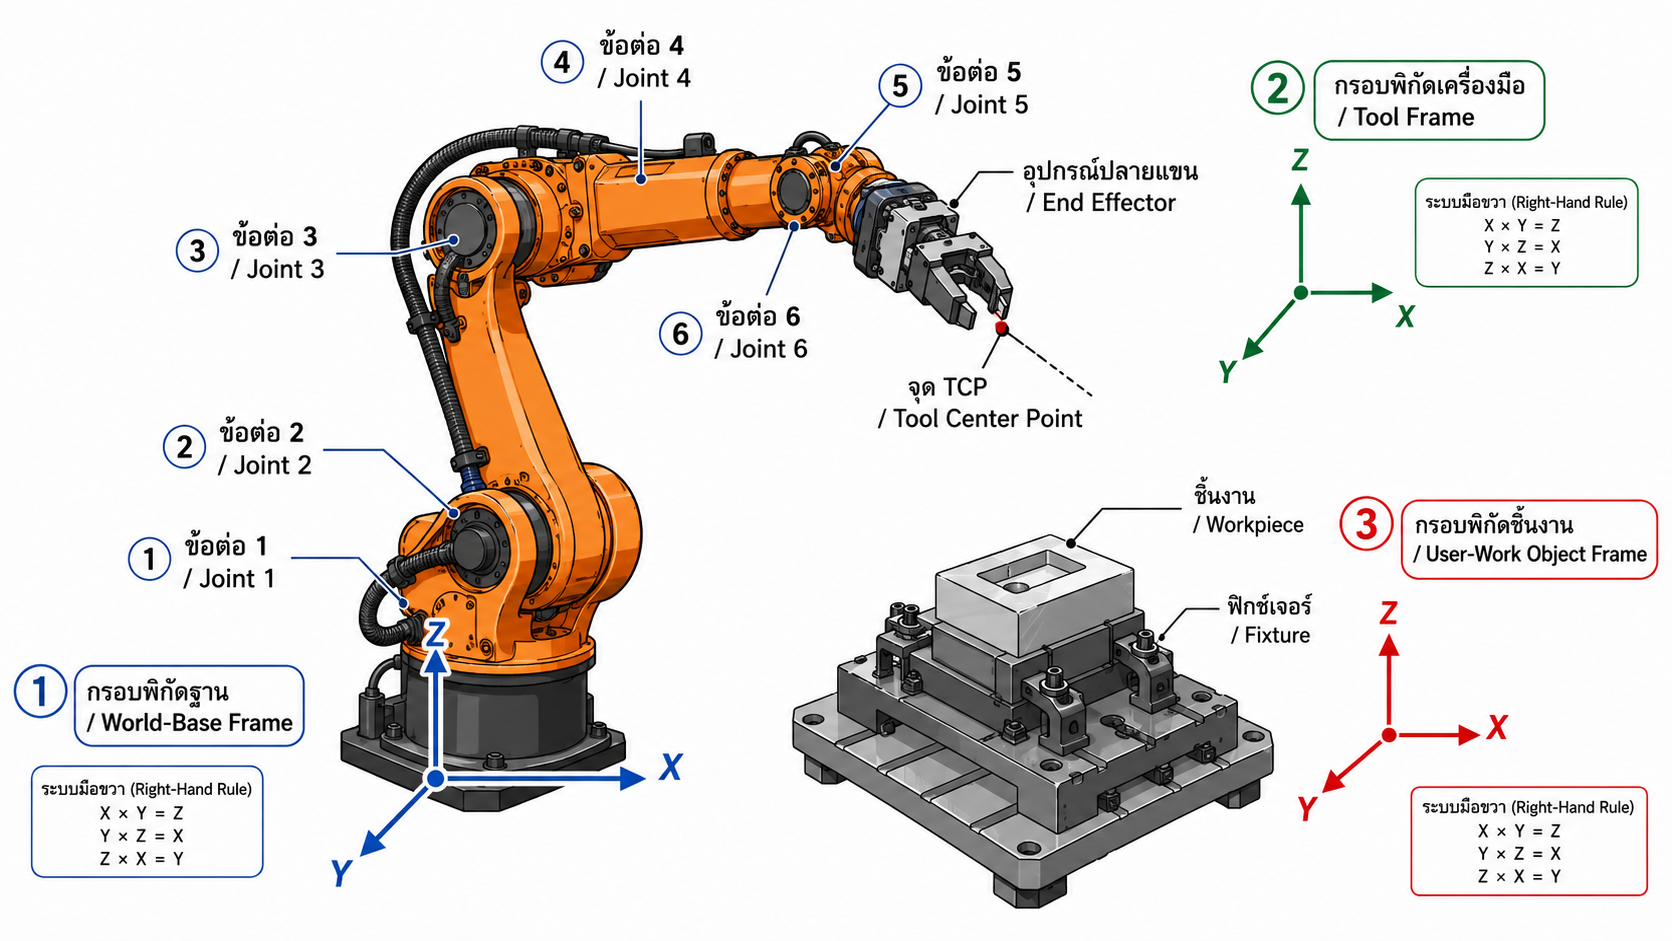
\includegraphics[width=0.8\textwidth]{images/chapter8/figure-01.png}
    \caption{ระบบพิกัด World, Tool และ User บนหุ่นยนต์ 6 แกน}
\end{figure}

\par\noindent\rule{\textwidth}{0.4pt}\par
\subsection{7.2 วิธีการสอนตำแหน่งหุ่นยนต์}

\subsubsection{7.2.1 Online Teaching ด้วย Teach Pendant}

Online Teaching คือการใช้ Controller และหุ่นยนต์จริงเพื่อสอนจุดหรือปรับโปรแกรมโดยตรง วิธีนี้ให้ข้อมูลจากระบบจริง เช่น Reachability, Joint Limit, Cable Routing, Fixture Clearance และพฤติกรรมของ End Effector แต่ทำให้เซลล์ไม่สามารถผลิตได้ในช่วงที่สอนและมีความเสี่ยงจากการเคลื่อนที่จริง

ลำดับการสอนตำแหน่งที่แนะนำมีดังนี้

\begin{enumerate}
    \item \textbf{ตรวจสอบพื้นที่และสถานะระบบ} — ไม่มีบุคคลหรือสิ่งของที่ไม่เกี่ยวข้องในพื้นที่ กำหนดผู้ควบคุม Teach Pendant เพียงคนเดียว
    \item \textbf{เลือก Operating Mode ที่เหมาะสม} — ใช้โหมด Manual/Teach แบบลดความเร็วตามข้อกำหนดของระบบฝึก
    \item \textbf{ตรวจสอบ Enabling Device} — ผู้สอนต้องเข้าใจตำแหน่งปล่อย กดกึ่งกลาง และกดสุดของอุปกรณ์
    \item \textbf{เลือก Tool และ User Frame} — ตรวจหมายเลข Tool/User ที่ Active ก่อน Jog
    \item \textbf{เลือก Coordinate System} — Joint, World, Tool หรือ User ตามเจตนาการเคลื่อนที่
    \item \textbf{เริ่มด้วยความเร็วต่ำ} — โดยเฉพาะเมื่ออยู่ใกล้ Fixture, Tool, Cable หรือ Singularity
    \item \textbf{Jog ไปยัง Approach Position} — ใช้จุดเหนือหรือห่างจากชิ้นงานก่อนเข้าสู่ตำแหน่งทำงาน
    \item \textbf{เข้าสู่ Work Position อย่างควบคุม} — ใช้ Tool หรือ User Coordinate เพื่อรักษาทิศทางที่เข้าใจง่าย
    \item \textbf{บันทึก Point} — ตั้งชื่อหรือหมายเลขให้สื่อความหมาย เช่น \texttt{P\_PICK\_APP}, \texttt{P\_PICK}, \texttt{P\_PLACE\_APP}
    \item \textbf{ตรวจสอบค่าที่บันทึก} — Frame, Tool, Configuration, Turn Number และ Motion Type
    \item \textbf{ทดสอบแบบ Step/Single Block} — เริ่มจากความเร็ว Override ต่ำและไม่มีชิ้นงาน
    \item \textbf{บันทึก Backup} — หลังการแก้โปรแกรมหรือ Frame ที่ผ่านการทวนสอบ
\end{enumerate}

\textbf{แนวคิด Approach–Process–Retreat}

การสอนจุดหนึ่งงานควรแยกอย่างน้อยเป็น 3 กลุ่ม

\begin{itemize}
    \item \textbf{Approach Point:} จุดปลอดภัยก่อนเข้าใกล้ชิ้นงาน
    \item \textbf{Process Point:} จุดที่ทำงานจริง เช่น Pick, Weld Start หรือ Inspection
    \item \textbf{Retreat Point:} จุดถอยออกจากชิ้นงานตามแนวที่ลดโอกาสชน
\end{itemize}

การใช้จุดเดียวทั้งเข้าและออกอาจเหมาะกับงานง่าย แต่ในงานที่มี Fixture ลึกหรือมีชิ้นส่วนยื่น การแยกจุดช่วยให้ Recovery และการวิเคราะห์ Collision ทำได้ชัดเจนกว่า

\subsubsection{7.2.2 Lead-through Programming}

Lead-through หรือ Hand Guiding คือการนำแขนหุ่นยนต์ด้วยมือในระบบที่ได้รับการออกแบบให้รองรับ เช่น Collaborative Robot หรือหุ่นยนต์ที่มีโหมด Hand Guiding และแรงชดเชยน้ำหนักจากผู้ผลิต การใช้งานทั่วไปประกอบด้วย

\begin{enumerate}
    \item เลือกโหมด Hand Guiding ที่ได้รับอนุญาต
    \item ตรวจสอบ Tool Payload, Center of Gravity และ TCP
    \item กดอุปกรณ์อนุญาตหรือปุ่ม Freedrive ตามระบบ
    \item นำ TCP ไปยัง Pose ที่ต้องการ
    \item บันทึก Waypoint หรือบันทึกเส้นทาง
    \item ปรับ Speed, Acceleration, Blend และ Orientation ในโปรแกรม
    \item จำลองหรือเล่นกลับที่ความเร็วต่ำ
\end{enumerate}

\textbf{ข้อจำกัดสำคัญ}

\begin{itemize}
    \item ไม่ใช่หุ่นยนต์ทุกชนิดที่อนุญาตให้ปลด Brake แล้วดึงแขนด้วยมือ
    \item การปลด Brake เพื่อ Service ไม่เท่ากับโหมด Hand Guiding สำหรับ Programming
    \item เส้นทางที่บันทึกด้วยมืออาจมี Noise จุดมากเกินไป หรือ Orientation ไม่สม่ำเสมอ
    \item ต้องประเมิน Pinch Point, Tool Hazard และแรงจาก Payload แม้เป็น Cobot
\end{itemize}

\subsubsection{7.2.3 Offline Programming}

Offline Programming (OLP) คือการสร้างโปรแกรม เส้นทาง และ Cell Layout บนคอมพิวเตอร์ โดยใช้ Robot Model และ Virtual Controller เมื่อเหมาะสม ตัวอย่างซอฟต์แวร์จากผู้ผลิต ได้แก่ FANUC ROBOGUIDE, ABB RobotStudio, KUKA.Sim หรือแพลตฟอร์มรุ่นใหม่ของ KUKA, Yaskawa MotoSim, Mitsubishi RT ToolBox3 และ Universal Robots URSim

\textbf{ขั้นตอน OLP ที่เป็นระบบ}

\begin{enumerate}
    \item นำเข้า CAD ของหุ่นยนต์ Fixture เครื่องจักร Tool และชิ้นงาน
    \item กำหนด Robot Base, External Axis และ Tool Geometry
    \item กำหนด TCP, Payload และ Work Object/User Frame
    \item สร้าง Targets และ Path
    \item เลือก Motion Type, Speed, Zone/Blend และ Process Parameters
    \item ตรวจ Reachability, Joint Limit, Singularity และ Collision
    \item ประมาณ Cycle Time
    \item สร้างหรือ Synchronize Program กับ Virtual Controller
    \item Export โปรแกรมตามรูปแบบที่ Controller รองรับ
    \item ทำ On-site Touch-up เพื่อชดเชยความคลาดเคลื่อนระหว่าง CAD กับระบบจริง
    \item ทดสอบใน Manual Reduced-speed ก่อน Automatic Mode
\end{enumerate}

\textbf{ข้อดี}

\begin{itemize}
    \item ลดเวลาที่ต้องหยุดสายการผลิต
    \item ตรวจ Collision และ Reachability ก่อนติดตั้งจริง
    \item ทดลอง Layout หลายทางเลือกได้
    \item ใช้สร้างสื่อการสอนและฝึกผู้เรียนโดยไม่เสี่ยงต่ออุปกรณ์จริง
    \item สนับสนุน Virtual Commissioning และการประเมิน Cycle Time
\end{itemize}

\textbf{ข้อจำกัด}

\begin{itemize}
    \item คุณภาพผลลัพธ์ขึ้นกับความถูกต้องของ CAD, Tool, Payload, Base และ Calibration
    \item Flexible Cable, Backlash, Thermal Drift และ Fixture Tolerance อาจไม่ถูกจำลองครบ
    \item Collision-free ใน Simulation ไม่ได้หมายความว่าปลอดภัยในระบบจริง
    \item Controller Option และ Software Version ต้องสอดคล้องกับหุ่นยนต์จริง
\end{itemize}

\subsubsection{ตาราง 8.3 เปรียบเทียบ Online, Lead-through และ Offline Programming}

\begin{table}[htbp]
    \centering
    \small
    \begin{tabularx}{\textwidth}{@{}L{0.17\textwidth}L{0.26\textwidth}L{0.28\textwidth}Y@{}}
        \hline
        \textbf{วิธี} & \textbf{จุดเด่น} & \textbf{ข้อจำกัด} & \textbf{งานที่เหมาะสม} \\
        \hline
        Teach Pendant & สอดคล้องกับระบบจริง เห็น Clearance จริง & ใช้เวลาหุ่นยนต์จริงและมีความเสี่ยง & Touch-up, Recovery, งานจุดไม่มาก \\
        Lead-through & เรียนรู้ง่าย เหมาะกับท่าทางเชิงสาธิต & ขึ้นกับรุ่นหุ่นยนต์และอาจได้เส้นทางไม่เรียบ & Cobot, งานสาธิต, งาน Path แบบง่าย \\
        Offline Programming & ลด Downtime ตรวจ Collision และ Cycle Time & ต้องมี Model และ Calibration ที่ดี & Welding, Painting, Machining, Cell ใหม่ \\
        \hline
    \end{tabularx}
\end{table}

\subsubsection{7.2.4 การกำหนดคุณภาพของจุดสอน}

จุดที่ดีไม่ได้หมายถึงเพียง TCP อยู่ตำแหน่งถูกต้อง แต่ต้องมีองค์ประกอบต่อไปนี้

\begin{itemize}
    \item Tool Frame และ User Frame ถูกต้อง
    \item Orientation เหมาะกับกระบวนการ
    \item Robot Configuration ไม่เปลี่ยนโดยไม่ตั้งใจ
    \item มีระยะเผื่อจาก Joint Limit และ Singularity
    \item สาย Tool และ Dress Pack ไม่บิดตึง
    \item Approach/Retreat ไม่ตัดผ่าน Fixture
    \item สามารถ Recover ได้เมื่อหยุดกลาง Cycle
    \item ชื่อ Point และ Comment สื่อความหมาย
    \item Point สำคัญที่ต้องสัมผัสชิ้นงานใช้ Fine/Exact Stop ตามความจำเป็น
    \item จุดผ่านที่ใช้เพิ่มความต่อเนื่องไม่ทำให้ Path เบี่ยงเข้าหาสิ่งกีดขวาง
\end{itemize}

\subsubsection{Checklist ก่อนบันทึกจุด}

\begin{verbatim}
[ ] Tool Number ถูกต้อง
[ ] User/Work Object Number ถูกต้อง
[ ] Coordinate System ตรงกับงาน
[ ] Speed Override อยู่ในระดับปลอดภัย
[ ] TCP และส่วนอื่นของแขนมี Clearance
[ ] Orientation ไม่ทำให้สายบิด
[ ] Joint อยู่ห่างจาก Limit และ Singularity
[ ] ตั้งชื่อ Point และ Comment แล้ว
[ ] กำหนด Motion Type และ Termination เหมาะสม
\end{verbatim}

\par\noindent\rule{\textwidth}{0.4pt}\par

\subsection{7.3 Motion Commands และการวางแผนเส้นทาง}

\subsubsection{7.3.1 ความแตกต่างระหว่าง Path และ Trajectory}

\begin{itemize}
    \item \textbf{Path} คือรูปร่างทางเรขาคณิตที่ TCP หรือ Joint เคลื่อนผ่าน โดยยังไม่ระบุเวลา
    \item \textbf{Trajectory} คือ Path ที่กำหนดเวลา ความเร็ว ความเร่ง และอาจรวม Jerk
\end{itemize}

โปรแกรมอาจกำหนดจุดต้นและจุดปลายเหมือนกัน แต่ให้ Trajectory ต่างกันจาก Motion Type, Speed, Acceleration, Payload และ Blending ดังนั้นการประเมินคุณภาพต้องพิจารณาทั้งตำแหน่งและพฤติกรรมตามเวลา

\subsubsection{7.3.2 Point-to-Point Motion: PTP}

PTP วางแผนการเคลื่อนที่ใน Joint Space โดยให้แต่ละ Joint เปลี่ยนจากค่าเริ่มต้นไปยังค่าปลาย หุ่นยนต์จะประสานเวลาให้แกนต่าง ๆ ถึงเป้าหมายตามแผนของ Controller รูปแบบเชิงแนวคิดเขียนได้เป็น

\[
q_i(t)=q_{i,0}+s(t)(q_{i,f}-q_{i,0})
\]

เมื่อ

\begin{itemize}
    \item $q_{i,0}$ คือค่าข้อต่อเริ่มต้น
    \item $q_{i,f}$ คือค่าข้อต่อปลาย
    \item $s(t)$ คือฟังก์ชันการเคลื่อนที่ที่เปลี่ยนจาก 0 เป็น 1
\end{itemize}

Controller จริงอาจใช้โปรไฟล์ความเร็วแบบ Trapezoidal, S-curve หรือวิธีเฉพาะของผู้ผลิต

\textbf{ข้อดี}

\begin{itemize}
    \item คำนวณได้มีประสิทธิภาพและมักเคลื่อนที่ได้เร็ว
    \item เหมาะสำหรับการเคลื่อนระหว่างจุดที่ไม่ต้องควบคุมรูปร่างเส้นทาง
    \item ใช้สำหรับ Home, Transfer หรือ Approach ที่มีพื้นที่ว่างเพียงพอ
\end{itemize}

\textbf{ข้อจำกัด}

\begin{itemize}
    \item เส้นทาง TCP ไม่รับประกันเป็นเส้นตรง
    \item ส่วนต่าง ๆ ของแขนอาจกวาดผ่านพื้นที่กว้าง
    \item ไม่เหมาะกับงานเชื่อม เดินกาว ตัด หรือพ่นที่ต้องควบคุม Path
\end{itemize}

ตัวอย่างคำสั่ง

\begin{verbatim}
FANUC: J P[1] 100% FINE
ABB:   MoveJ Target1, v1000, fine, tool1;
KUKA:  PTP P1
Yaskawa: MOVJ P001 VJ=50.00
URScript: movej(q_target, a=1.2, v=0.8)
\end{verbatim}

\begin{quote}
รูปแบบคำสั่งเป็นตัวอย่างเชิงการเรียนรู้ ต้องตรวจ Syntax, Unit และ Option จากคู่มือ Controller รุ่นที่ใช้งาน
\end{quote}

\subsubsection{7.3.3 Linear Motion: LIN}

Linear Motion ควบคุมให้ TCP เคลื่อนตามเส้นตรงจากตำแหน่งเริ่ม $\mathbf{p}_0$ ไปยังตำแหน่งปลาย $\mathbf{p}_f$

\[
\mathbf{p}(t)=\mathbf{p}_0+s(t)(\mathbf{p}_f-\mathbf{p}_0)
\]

Controller ต้องคำนวณ Inverse Kinematics หลายครั้งตามเส้นทาง เพื่อหาค่า Joint ที่ทำให้ TCP อยู่บนเส้นตรงและ Orientation เปลี่ยนตามกฎที่กำหนด

\textbf{เหมาะสำหรับ}

\begin{itemize}
    \item เข้า–ออกชิ้นงานตามแนว Tool
    \item งานเชื่อมแนวตรง เดินกาว ตัด และตรวจสอบ
    \item งานหยิบวางที่ต้องหลีกเลี่ยงขอบ Fixture
    \item การเคลื่อนชิ้นงานที่ต้องรักษาระดับหรือ Orientation
\end{itemize}

\textbf{ข้อจำกัด}

\begin{itemize}
    \item อาจผ่าน Singularity หรือ Joint Limit แม้จุดต้นและปลายเข้าถึงได้
    \item ความเร็ว TCP สูงอาจต้องการความเร็ว Joint สูงมากในบางท่าทาง
    \item ใช้ทรัพยากรการคำนวณและข้อจำกัดของ Controller มากกว่า PTP
\end{itemize}

\begin{verbatim}
FANUC: L P[2] 500mm/sec FINE
ABB:   MoveL Target2, v500, z10, tool1;
KUKA:  LIN P2
Yaskawa: MOVL P002 V=500.0
URScript: movel(p_target, a=0.5, v=0.25)
\end{verbatim}

\subsubsection{7.3.4 Circular Motion: CIRC/ARC}

การเคลื่อนที่เป็นวงโค้งต้องมีอย่างน้อยจุดเริ่ม จุดผ่าน และจุดปลาย เพื่อกำหนดระนาบและส่วนโค้ง

\begin{verbatim}
FANUC: C P[3] P[4] 500mm/sec FINE
ABB:   MoveC CirPoint, Target3, v500, z10, tool1;
KUKA:  CIRC P3, P4
Yaskawa: MOVC P003 V=300.0
URScript: movec(p_via, p_to, a=0.5, v=0.2)
\end{verbatim}

\textbf{การประยุกต์ใช้} ได้แก่ การเชื่อมตามท่อ งานขัดขอบโค้ง งานพ่นสี และการเคลื่อนรอบชิ้นงานทรงกระบอก

\textbf{ข้อควรระวัง}

\begin{itemize}
    \item จุดทั้งสามต้องไม่เกือบอยู่บนเส้นตรงเดียวกัน
    \item Orientation ระหว่างจุดต้องถูกกำหนดให้เหมาะสมกับกระบวนการ
    \item หาก Arc ใหญ่หรือซับซ้อน ควรแบ่งเป็นหลายส่วนและตรวจ Continuity
\end{itemize}

\subsubsection{7.3.5 Blending, Zone และ CNT}

หากกำหนดจุดเป็น Fine/Exact Stop หุ่นยนต์จะลดความเร็วจนเข้าเกณฑ์ตำแหน่งก่อนเริ่ม Motion ถัดไป การหยุดทุกจุดเพิ่ม Cycle Time และทำให้ความเร่งเปลี่ยนบ่อย ในทางกลับกัน Blending ทำให้ Controller เริ่มเบี่ยงจากจุดเดิมเพื่อเชื่อมกับเส้นทางถัดไปอย่างต่อเนื่อง

\begin{table}[htbp]
    \centering
    \begin{tabular}{l l r r}
        \hline
        \textbf{ค่าตัวอย่าง} & \textbf{พฤติกรรมโดยแนวคิด} & \textbf{ผลต่อ Cycle Time} & \textbf{ผลต่อความแม่นยำผ่านจุด} \\
        \hline
        FINE / fine & เข้าเป้าหมายตามเกณฑ์แล้วจึงไปต่อ & สูง & สูง \\
        CNT 0 หรือ Zone ใกล้ศูนย์ & เกือบหยุดหรือเบี่ยงน้อย & ค่อนข้างสูง & ค่อนข้างสูง \\
        CNT 50 / Zone ปานกลาง & กลมมุมระดับกลาง & ลดลง & จุดผ่านคลาดมากขึ้น \\
        CNT 100 / Zone ใหญ่ & ต่อเนื่องสูง เบี่ยงจากจุดมาก & ต่ำ & ไม่เหมาะกับจุดกระบวนการสำคัญ \\
        \hline
    \end{tabular}
\end{table}

\textbf{หลักการเลือก}

\begin{itemize}
    \item จุด Pick, Place, Tool Change, Probe และจุดที่รอสัญญาณควรใช้ Fine หรือ Zone ต่ำ
    \item จุดผ่านกลางอากาศที่มี Clearance มากอาจใช้ Blend สูง
    \item ห้ามเพิ่ม Blend โดยดูเฉพาะ Cycle Time ต้องตรวจ Swept Volume ของ TCP และทุก Link
    \item Path ที่มุมแหลมมากอาจไม่สามารถรักษาความเร็วคงที่ได้ แม้กำหนด Blend
\end{itemize}

\subsubsection{ตัวอย่างที่ 8.2 ผลของการหยุดต่อ Cycle Time}

\textbf{ตัวอย่างเพิ่มเติมเพื่อการเรียนรู้}

โปรแกรมมีจุดผ่านกลางอากาศ 4 จุด หากใช้ Fine ทุกจุด หุ่นยนต์ใช้เวลาเร่งและลดความเร็วเพิ่มจุดละ 0.25 s เมื่อเปลี่ยนจุดผ่านทั้ง 4 เป็น Blend ที่ผ่านการตรวจ Collision แล้ว จะลดเวลาได้โดยประมาณเท่าใด

\[
\Delta t = 4(0.25)=1.00\text{ s/cycle}
\]

ถ้าผลิต 3,600 Cycle ต่อวัน เวลาที่ลดได้คือ

\[
1.00\times 3600=3600\text{ s}=60\text{ min/day}
\]

\textbf{การแปลความหมาย:} การปรับ Motion Termination ที่จุดไม่สำคัญสามารถเพิ่มกำลังการผลิตได้มาก แต่ต้องยืนยันว่า Path ใหม่ไม่เข้าใกล้คน อุปกรณ์ หรือชิ้นงานเกินเกณฑ์

\subsubsection{7.3.6 ปัจจัยที่มีผลต่อ Path Planning}

\begin{enumerate}
    \item \textbf{Reachability:} จุดต้องอยู่ใน Working Envelope และไม่เกิน Joint Limit
    \item \textbf{Robot Configuration:} Shoulder, Elbow, Wrist และ Turn Number ต้องสอดคล้องตลอดเส้นทาง
    \item \textbf{Singularity:} ควรหลีกเลี่ยงท่าที่ต้องการความเร็ว Joint สูงผิดปกติ
    \item \textbf{Payload และ Center of Gravity:} มีผลต่อ Acceleration, Braking และ Alarm Overload
    \item \textbf{Tool Geometry:} ต้องตรวจทั้ง TCP และ Volume ของ Tool
    \item \textbf{Dress Pack:} สายไฟ สายลม และสายเชื่อมต้องไม่ตึงหรือเสียดสี
    \item \textbf{Fixture Clearance:} ต้องรวม Tolerance, Deflection และตำแหน่งชิ้นงานจริง
    \item \textbf{Process Requirement:} งานเชื่อมและพ่นต้องควบคุม Speed และ Orientation ต่อเนื่อง
    \item \textbf{Recovery:} ต้องมีจุดหรือขั้นตอนถอยออกเมื่อ Cycle หยุดกลางทาง
    \item \textbf{Safety Zone:} เส้นทางต้องอยู่ภายในข้อจำกัดของ Safety Function และพื้นที่อนุญาต
\end{enumerate}

\subsubsection{ตาราง 8.4 แนวทางเลือก Motion ตามงาน}

\begin{table}[htbp]
    \centering
    \begin{tabular}{l l l l}
        \hline
        \textbf{สถานการณ์} & \textbf{Motion แนะนำ} & \textbf{Termination} & \textbf{เหตุผล} \\
        \hline
        เคลื่อนจาก Home ไปเหนือจุด Pick & PTP/J & Blend ปานกลางเมื่อมี Clearance & ลด Cycle Time \\
        ลงจับชิ้นงานใน Fixture & Linear & Fine & รักษาแนวเข้าและตำแหน่งจับ \\
        ถอย Gripper ออกจากชิ้นงาน & Linear & Blend ต่ำหรือ Fine & ลดการเฉี่ยวชิ้นงาน \\
        เคลื่อนระหว่างพื้นที่ว่าง & PTP/J & Blend สูงตามการตรวจสอบ & เร็วและใช้เส้นทาง Joint \\
        เชื่อมแนวตรง & Linear & Zone ต่อเนื่องตาม Process & รักษาความเร็วและแนวเชื่อม \\
        เชื่อมแนวโค้ง & Circular & Zone ที่ไม่ทำลายรูปทรง & รักษา Arc และความต่อเนื่อง \\
        เข้า Tool Changer & Linear & Fine & ต้องจัดแนวและล็อกอย่างแม่นยำ \\
        \hline
    \end{tabular}
\end{table}

% [รูปที่ 8.2: เปรียบเทียบเส้นทาง PTP และ Linear]
% ประเภทภาพ: Technical Illustration
% ตำแหน่งที่แนะนำ: หลังหัวข้อ 7.3.3
% วัตถุประสงค์การเรียนรู้: ให้เห็นว่า PTP ไม่รับประกันเส้นทาง TCP ขณะที่ LIN ควบคุมเส้นตรง
% คำอธิบายภาพ: จุด A และ B เดียวกัน มีเส้นโค้งของ TCP สำหรับ PTP และเส้นตรงสำหรับ LIN พร้อมภาพท่าหุ่นยนต์ระหว่างทาง
% องค์ประกอบที่ต้องมี: Robot poses, Point A, Point B, curved PTP path, straight LIN path, obstacle clearance
% ข้อความหรือป้ายกำกับ: PTP/Joint-space, LIN/Cartesian straight line
% ภาษาของป้ายกำกับ: ไทยและอังกฤษ
% สัดส่วนภาพ: 16:9
% Image Generation Prompt: Clean engineering textbook comparison of a six-axis industrial robot moving between the same point A and point B. Left panel shows point-to-point joint-space motion with a curved and uncontrolled TCP path. Right panel shows linear Cartesian motion with a straight TCP path. Include intermediate robot poses, an obstacle for clearance context, arrows and bilingual Thai-English labels. White background, precise vector style, 16:9.
% Alt Text: ภาพเปรียบเทียบเส้นทาง TCP แบบโค้งของ PTP กับเส้นตรงของ Linear Motion

\begin{figure}[htbp]
    \centering
    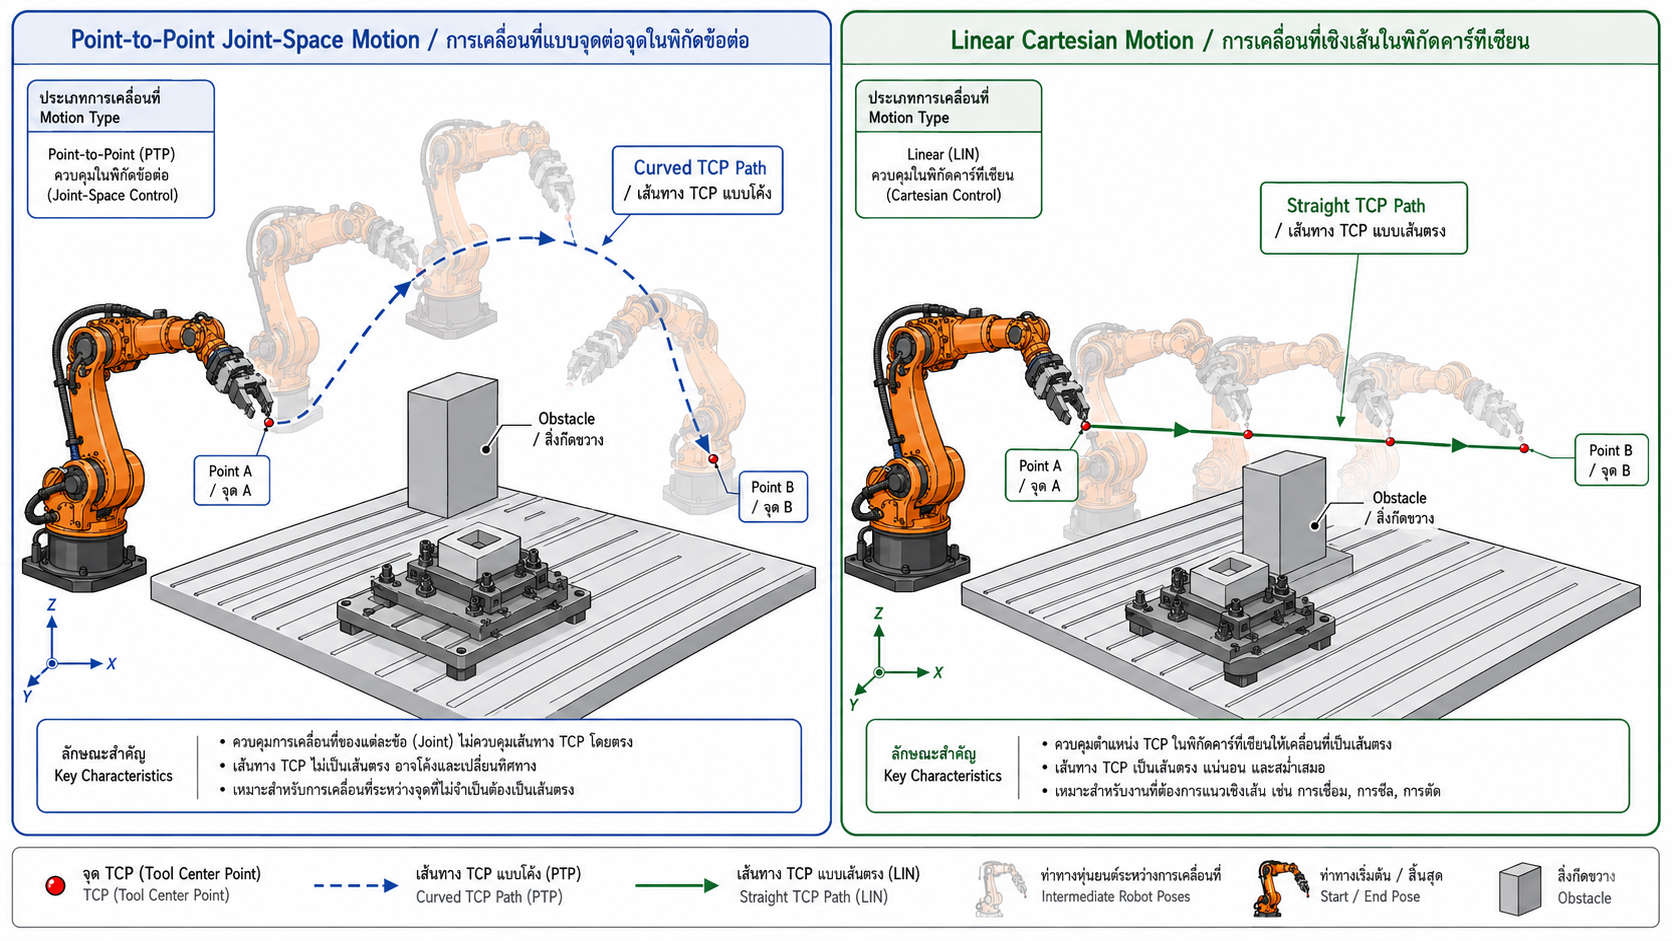
\includegraphics[width=0.8\textwidth]{images/chapter8/figure-02.png}
    \caption{เปรียบเทียบเส้นทาง PTP และ Linear}
\end{figure}

% [รูปที่ 8.3: ผลของ FINE และ CNT/Zone Blending]
% ประเภทภาพ: Technical Diagram
% ตำแหน่งที่แนะนำ: หลังหัวข้อ 7.3.5
% วัตถุประสงค์การเรียนรู้: แสดงการเบี่ยงจากจุดผ่านเมื่อเพิ่มระดับ Blending
% คำอธิบายภาพ: เส้นทางหักมุมผ่าน P1–P2–P3 เปรียบเทียบ FINE, Blend ต่ำ, Blend กลาง และ Blend สูง
% องค์ประกอบที่ต้องมี: จุด P1 P2 P3, exact path, four rounded paths, deviation distance and velocity arrows
% ข้อความหรือป้ายกำกับ: FINE, CNT/Zone Low, Medium, High, Path Deviation
% ภาษาของป้ายกำกับ: ไทยและอังกฤษ
% สัดส่วนภาพ: 16:9
% Image Generation Prompt: Engineering path diagram showing a robot TCP moving through three points P1, P2 and P3 with a sharp corner at P2. Compare four trajectories: FINE exact stop, low blend, medium blend and high blend. Show increasing corner radius, path deviation and smoother velocity continuity. Clean white background, precise vector lines, bilingual Thai-English labels, 16:9.
% Alt Text: เส้นทางผ่านสามจุดที่มีการกลมมุมเพิ่มขึ้นจาก FINE ไปยัง Blend สูง

\begin{figure}[htbp]
    \centering
    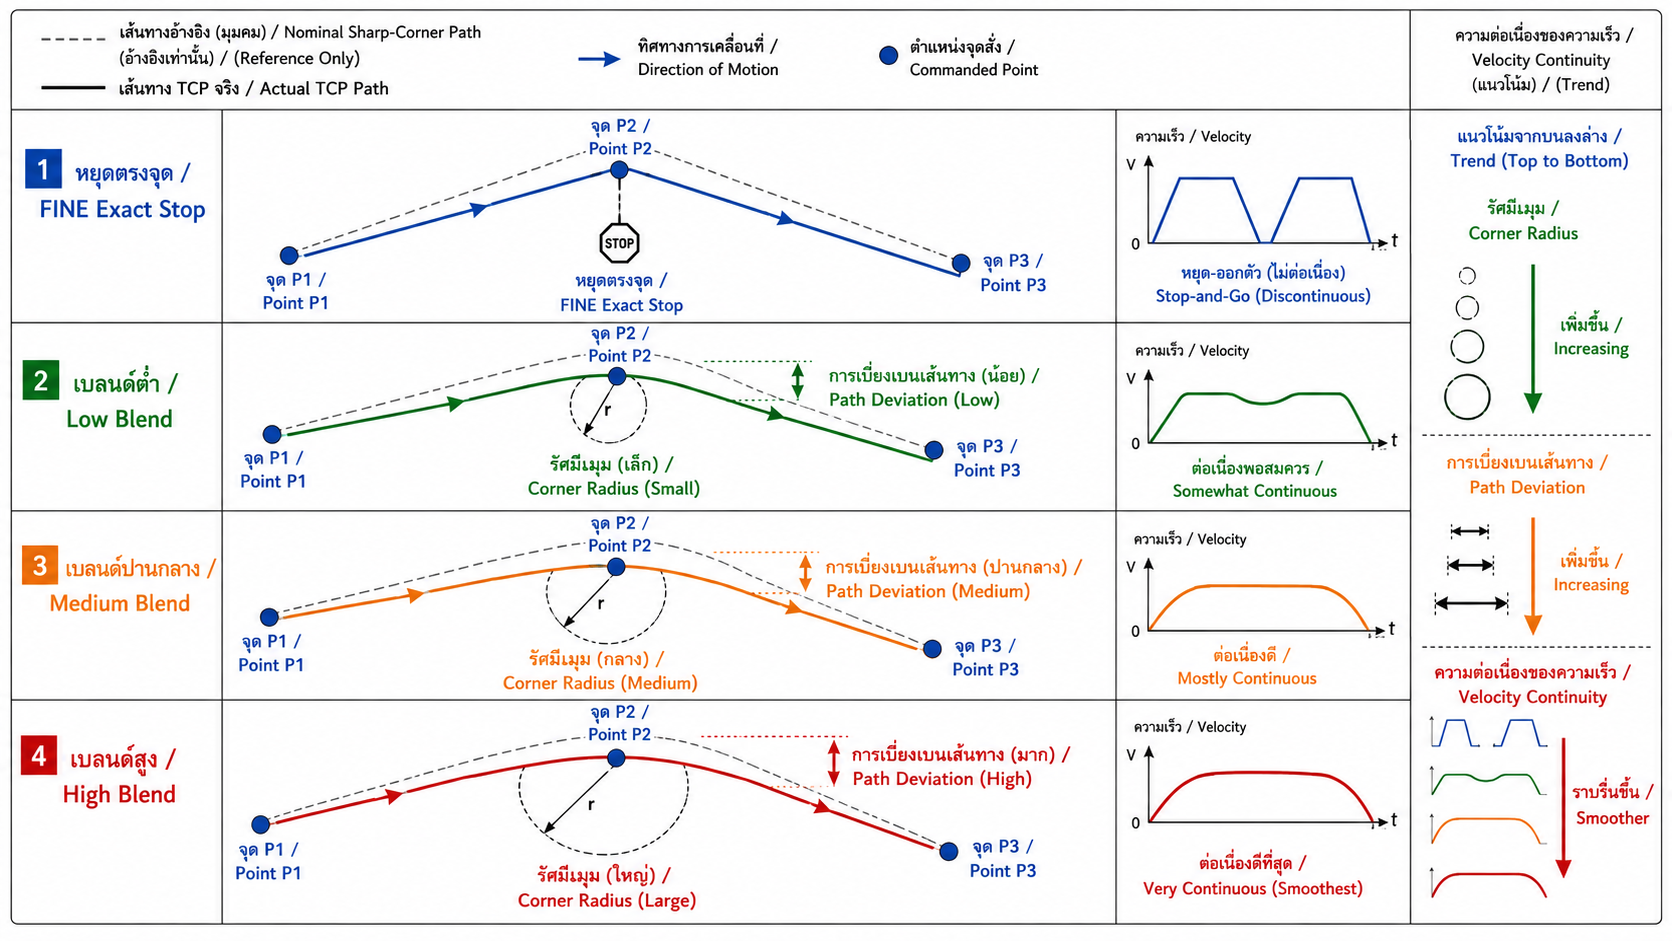
\includegraphics[width=0.8\textwidth]{images/chapter8/figure-03.png}
    \caption{ผลของ FINE และ CNT/Zone Blending}
\end{figure}

\par\noindent\rule{\textwidth}{0.4pt}\par

\subsection{7.4 โครงสร้างโปรแกรมหุ่นยนต์เบื้องต้น}

\subsubsection{7.4.1 องค์ประกอบของโปรแกรมที่อ่านและบำรุงรักษาได้}

โปรแกรมหุ่นยนต์ที่ดีควรแยกองค์ประกอบต่อไปนี้

\begin{enumerate}
    \item \textbf{Configuration:} หมายเลข Tool, User Frame, Payload, Speed Override และ Process Mode
    \item \textbf{Position Data:} Home, Approach, Process, Retreat, Recovery และ Maintenance Position
    \item \textbf{Motion Logic:} ลำดับ J/L/C หรือ MoveJ/MoveL/MoveC
    \item \textbf{I/O Logic:} Gripper, Clamp, Sensor, Conveyor, Machine Ready และ Safety-permissive interface
    \item \textbf{Control Flow:} IF, SELECT, LOOP, FOR, CALL, WAIT, TIMER และ Label
    \item \textbf{Fault Handling:} Timeout, Retry Limit, Alarm Message และ Safe Stop
    \item \textbf{Production Data:} Counter, Recipe, Part Type และ Result
    \item \textbf{Comments and Revision:} ผู้แก้ไข วันที่ เหตุผล และ Version
\end{enumerate}

\subsubsection{7.4.2 ตัวอย่างโปรแกรม Pick and Place แบบ FANUC TP-like}

\begin{verbatim}
1:  !--- PICK AND PLACE PROGRAM --- ;
2:  UFRAME_NUM=1 ;
3:  UTOOL_NUM=1 ;
4:  ! Verify cell conditions ;
5:  WAIT DI[1:CELL_READY]=ON ;
6:  WAIT DI[2:PART_PRESENT]=ON ;
7:  WAIT DI[3:PLACE_CLEAR]=ON ;
8:  ;
9:  !--- HOME POSITION --- ;
10: J P[1:HOME] 50% FINE ;
11: ;
12: !--- APPROACH PICK --- ;
13: J P[2:PICK_APP] 50% CNT50 ;
14: L P[3:PICK] 150mm/sec FINE ;
15: DO[1:GRIP_CLOSE]=ON ;
16: WAIT DI[4:GRIP_OK]=ON TIMEOUT,LBL[900] ;
17: L P[2:PICK_APP] 200mm/sec CNT20 ;
18: ;
19: !--- MOVE TO PLACE --- ;
20: J P[4:PLACE_APP] 50% CNT50 ;
21: L P[5:PLACE] 150mm/sec FINE ;
22: DO[1:GRIP_CLOSE]=OFF ;
23: WAIT DI[5:GRIP_OPEN]=ON TIMEOUT,LBL[910] ;
24: L P[4:PLACE_APP] 200mm/sec CNT20 ;
25: J P[1:HOME] 50% FINE ;
26: DO[2:CYCLE_COMPLETE]=ON ;
27: WAIT 0.10(sec) ;
28: DO[2:CYCLE_COMPLETE]=OFF ;
29: END ;
30: ;
31: LBL[900] ;
32: CALL GRIP_FAULT ;
33: END ;
34: LBL[910] ;
35: CALL RELEASE_FAULT ;
36: END ;
\end{verbatim}

\begin{quote}
โค้ดนี้เป็นตัวอย่างเพื่ออธิบายโครงสร้าง ไม่ใช่ไฟล์ที่รับรองว่าสามารถโหลดได้กับ Controller ทุก Version ชื่อคำสั่ง Timeout และรูปแบบ Label ต้องปรับตามคู่มือจริง
\end{quote}

\subsubsection{7.4.3 ลำดับ Handshake กับ PLC}

การเชื่อมต่อหุ่นยนต์กับ PLC ควรใช้ State หรือ Handshake ที่ตรวจสอบได้ ไม่ควรใช้ Pulse สั้นโดยไม่มีการยืนยัน ตัวอย่างสัญญาณ ได้แก่

\begin{table}[htbp]
    \centering
    \begin{tabular}{l l}
        \hline
        \textbf{สัญญาณจาก PLC ไป Robot} & \textbf{ความหมาย} \\
        \hline
        \texttt{CELL\_READY} & อุปกรณ์รอบเซลล์อยู่ในสถานะพร้อม \\
        \texttt{START\_REQUEST} & ขอให้หุ่นยนต์เริ่ม Cycle \\
        \texttt{PART\_PRESENT} & มีชิ้นงานที่จุด Pick \\
        \texttt{PLACE\_CLEAR} & ตำแหน่งวางว่างและปลอดภัย \\
        \texttt{RESET\_REQUEST} & ขอ Reset หลังเงื่อนไขปลอดภัยครบ \\
        \hline
    \end{tabular}
\end{table}

\begin{table}[htbp]
    \centering
    \begin{tabular}{l l}
        \hline
        \textbf{สัญญาณจาก Robot ไป PLC} & \textbf{ความหมาย} \\
        \hline
        \texttt{ROBOT\_READY} & Robot อยู่ Home/Ready และไม่มี Fault \\
        \texttt{ROBOT\_BUSY} & กำลังทำ Cycle \\
        \texttt{CYCLE\_COMPLETE} & Cycle สำเร็จ \\
        \texttt{ROBOT\_FAULT} & มี Fault ต้องดำเนินการ \\
        \texttt{GRIP\_RESULT} & ผลการจับชิ้นงาน \\
        \hline
    \end{tabular}
\end{table}

ตัวอย่าง Sequence

\begin{verbatim}
PLC: START_REQUEST = ON
Robot: ตรวจ CELL_READY, PART_PRESENT, PLACE_CLEAR
Robot: ROBOT_BUSY = ON
Robot: ทำ Pick and Place
Robot: CYCLE_COMPLETE = ON
PLC: START_REQUEST = OFF และรับ Complete
Robot: CYCLE_COMPLETE = OFF, ROBOT_BUSY = OFF
\end{verbatim}

การออกแบบต้องกำหนดพฤติกรรมเมื่อสัญญาณค้าง สัญญาณหายระหว่าง Cycle หรือ Controller Restart เพื่อป้องกันการเริ่มซ้ำโดยไม่ตั้งใจ

\subsubsection{7.4.4 โครงสร้างควบคุมการไหล}

\begin{verbatim}
!--- IF CONDITION ---
IF DI[1:PART_OK] = ON THEN
  CALL PICK_ROUTINE
ELSE
  CALL EJECT_ROUTINE
ENDIF

!--- FOR LOOP ---
FOR R[1:INDEX] = 1 TO 10
  CALL CYCLE_ROUTINE
  R[2:GOOD_COUNT] = R[2:GOOD_COUNT] + 1
ENDFOR

!--- WAIT WITH TIMEOUT ---
WAIT DI[2:CLAMP_OK] = ON TIMEOUT LBL[100]
\end{verbatim}

\textbf{ข้อควรระวังของ Loop}

\begin{itemize}
    \item ต้องมีเงื่อนไขออกจาก Loop ที่ตรวจสอบได้
    \item ไม่ควร Retry การจับชิ้นงานไม่จำกัดครั้ง
    \item Counter ต้องถูก Initial เมื่อเริ่ม Lot หรือหลัง Recovery ตามกติกาที่ชัดเจน
    \item การ Restart ต้องรู้ว่า Cycle อยู่ State ใด ไม่ควรกลับไปเริ่มต้นโดยอัตโนมัติทุกกรณี
\end{itemize}

\subsubsection{7.4.5 ตัวอย่างโปรแกรมวางชิ้นงาน 2 × 5 ช่องแบบ Pseudocode}

\begin{verbatim}
SET ROWS = 2
SET COLS = 5
SET PITCH_X = 40 mm
SET PITCH_Y = 60 mm

FOR row = 0 TO ROWS-1
  FOR col = 0 TO COLS-1
    WAIT part_present = TRUE
    CALL PickPart()

    IF gripper_confirm = FALSE THEN
      RAISE "GRIPPER NOT CONFIRMED"
      STOP CYCLE
    ENDIF

    target = tray_origin
             + col * PITCH_X along User-X
             + row * PITCH_Y along User-Y

    MoveJ target_approach WITH blend
    MoveL target WITH fine
    OpenGripper()
    WAIT gripper_open = TRUE WITH timeout
    MoveL target_approach WITH low_blend
  ENDFOR
ENDFOR
\end{verbatim}

จุดเด่นของแนวทางนี้คือใช้จุดต้นเพียงจุดเดียวร่วมกับ Offset จึงลดจำนวน Point และทำให้ปรับ Pitch ได้ง่าย แต่ต้องตรวจว่า Offset ทุกจุดอยู่ใน Reach, ไม่เกิด Singularity และไม่ชนขอบถาด

\subsubsection{7.4.6 การจัดการ Timeout และ Fault}

การใช้ \texttt{WAIT} โดยไม่มี Timeout อาจทำให้โปรแกรมค้างโดยไม่ทราบสาเหตุ แนวทางที่ดีกว่าคือ

\begin{enumerate}
    \item เริ่ม Timer เมื่อส่งคำสั่งไปยังอุปกรณ์
    \item รอสัญญาณตอบกลับภายในเวลาที่กำหนด
    \item หากครบเวลา ให้หยุด Sequence ที่ปลอดภัย
    \item ปิด Output ที่อาจทำให้เกิดการเคลื่อนที่ต่อ
    \item แสดง Alarm ที่ระบุอุปกรณ์และ State
    \item ให้ผู้ปฏิบัติงานตรวจสาเหตุ
    \item อนุญาต Retry เมื่อเงื่อนไขปลอดภัยครบและจำนวนครั้งไม่เกินกำหนด
    \item บันทึกเหตุการณ์เพื่อวิเคราะห์ซ้ำ
\end{enumerate}

\subsubsection{7.4.7 การตรวจสอบโปรแกรมก่อนใช้งานจริง}

\textbf{ระดับที่ 1: Static Review}

\begin{itemize}
    \item Tool/User Frame ถูกต้อง
    \item Point Name และ Comment ชัดเจน
    \item Speed และ Termination เหมาะสม
    \item I/O Address ไม่ซ้ำหรือกลับ Logic
    \item Timeout และ Fault Path ครบ
    \item ไม่มี Jump/Label ที่ทำให้ข้าม Interlock
\end{itemize}

\textbf{ระดับที่ 2: Simulation}

\begin{itemize}
    \item Reachability และ Joint Limit
    \item Collision ของ Robot, Tool, Workpiece และ Fixture
    \item Cycle Time และ Bottleneck
    \item Singularity และ Configuration Change
\end{itemize}

\textbf{ระดับที่ 3: Dry Run บนหุ่นยนต์จริง}

\begin{itemize}
    \item ใช้ Manual Reduced-speed และ Step Mode
    \item ไม่มีชิ้นงานหรือใช้ชิ้นงานจำลองที่ปลอดภัย
    \item ผู้ควบคุมถือ Teach Pendant และสังเกต Clearance
    \item ตรวจทิศทาง Gripper/Actuator ก่อนจ่ายพลังงานเต็ม
\end{itemize}

\textbf{ระดับที่ 4: Process Validation}

\begin{itemize}
    \item ทดสอบด้วยชิ้นงานจริงภายใต้การควบคุม
    \item วัดคุณภาพ ตำแหน่ง Cycle Time และ Repeatability
    \item ทดสอบ Fault Scenario ที่ได้รับอนุญาต
    \item บันทึก Version และ Backup หลังอนุมัติ
\end{itemize}

\par\noindent\rule{\textwidth}{0.4pt}\par
\subsection{7.5 การบำรุงรักษาหุ่นยนต์อุตสาหกรรม}

\subsubsection{7.5.1 เป้าหมายของการบำรุงรักษา}

การบำรุงรักษาไม่ได้มีเป้าหมายเพียง “ซ่อมให้กลับมาทำงาน” แต่ต้องรักษาคุณลักษณะสำคัญของระบบ ได้แก่

\begin{itemize}
    \item ความปลอดภัยของผู้ปฏิบัติงาน
    \item ความพร้อมใช้งานของเซลล์
    \item ความแม่นยำและ Repeatability
    \item คุณภาพของกระบวนการ
    \item อายุของ Gear, Bearing, Brake, Cable และ Seal
    \item ความสมบูรณ์ของ Backup, Calibration และ Safety Configuration
    \item ความสามารถในการติดตามประวัติและวิเคราะห์สาเหตุซ้ำ
\end{itemize}

ประเภทการบำรุงรักษาที่พบ ได้แก่

\begin{enumerate}
    \item \textbf{Corrective Maintenance:} ซ่อมหลังเกิดความขัดข้อง
    \item \textbf{Preventive Maintenance:} ทำตามเวลา ชั่วโมงทำงาน หรือจำนวน Cycle
    \item \textbf{Condition-based Maintenance:} ทำเมื่อข้อมูลสภาพ เช่น อุณหภูมิ กระแสมอเตอร์ การสั่น หรือ Alarm Trend เปลี่ยน
    \item \textbf{Predictive Maintenance:} ใช้ข้อมูลและแบบจำลองคาดการณ์แนวโน้มความเสียหายก่อนหยุดเครื่อง
\end{enumerate}

ในห้องปฏิบัติการควรเน้น Preventive Maintenance และการตรวจสภาพพื้นฐาน ส่วนงาน Predictive Maintenance อาจสาธิตด้วยข้อมูล Trend หรือซอฟต์แวร์ Monitoring โดยไม่ดัดแปลงระบบจริง

\subsubsection{7.5.2 หลักการสร้างแผน PM}

แผน PM ที่ดีต้องตอบคำถาม 6 ข้อ

\begin{enumerate}
    \item \textbf{ตรวจอะไร} — เช่น Cable, Grease Leakage, Bolt, Fan, Filter, Battery และ Safety Device
    \item \textbf{ตรวจเมื่อใด} — รายวัน รายสัปดาห์ รายเดือน รายปี ชั่วโมงทำงาน หรือ Condition-based
    \item \textbf{ตรวจอย่างไร} — Visual, Torque Check, Functional Test, Measurement หรือ Trend Analysis
    \item \textbf{เกณฑ์ผ่านคืออะไร} — Normal/Abnormal, ค่าพิกัด, Tolerance หรือคำแนะนำผู้ผลิต
    \item \textbf{ใครรับผิดชอบ} — Operator, Maintenance Technician, Safety Specialist หรือผู้ผลิต
    \item \textbf{บันทึกที่ใด} — Checklist, CMMS, Logbook หรือระบบ Digital Maintenance
\end{enumerate}

\begin{quote}
\textbf{ข้อควรระวัง:} ระยะเปลี่ยน Grease, Battery, Belt, Seal และ Oil แตกต่างกันมากตามรุ่น ชั่วโมงทำงาน โหลด อุณหภูมิ และสภาพแวดล้อม ตารางต่อไปนี้เป็นโครงสร้างตัวอย่างเพื่อการเรียนรู้ ไม่ใช่คำสั่งบำรุงรักษาแทนคู่มือผู้ผลิต
\end{quote}

\subsubsection{ตาราง 8.5 แผน Preventive Maintenance ตัวอย่าง}

\begin{table}[htbp]
    \centering
    \small
    \begin{tabularx}{\textwidth}{@{}L{0.15\textwidth}L{0.20\textwidth}YL{0.19\textwidth}@{}}
        \hline
        \textbf{ความถี่ตัวอย่าง} & \textbf{กิจกรรม} & \textbf{รายละเอียดและเกณฑ์เบื้องต้น} & \textbf{ผู้รับผิดชอบ} \\
        \hline
        ก่อนเริ่มงานทุกวัน & Daily Visual Check & ตรวจรอยรั่ว Cable Damage ฝาครอบหลวม Tool หลวม เสียงผิดปกติ Air Pressure และ Alarm ค้าง & Operator \\
        ทุกสัปดาห์ & Functional Check & ทดสอบ Gripper Sensor, Interlock, Indicator และทำความสะอาดพื้นที่โดยไม่รบกวนอุปกรณ์นิรภัย & Operator/Technician \\
        ทุก 1–3 เดือน & Condition Inspection & ตรวจ Connector, Dress Pack, Fan/Filter, Bolt Mark, Backlash ที่สังเกตได้ และแนวโน้ม Alarm & Technician \\
        ตามชั่วโมงหรือคู่มือ & Lubrication Service & ใช้ชนิด ปริมาณ ตำแหน่ง และวิธีเติมตามคู่มือรุ่นนั้น ห้ามผสม Grease โดยไม่ยืนยันความเข้ากันได้ & Qualified Technician \\
        ทุกปีหรือรอบที่กำหนด & Annual Inspection & ตรวจ Brake, Cable, Safety Function, Calibration Status, Backup, Battery Condition และ Mechanical Wear & Qualified Technician \\
        ตามอายุ/สถานะ & Encoder/SMB Battery & เปลี่ยนตามคู่มือและขั้นตอนรักษาข้อมูลตำแหน่ง ห้ามตัดไฟผิดวิธี & Qualified Technician \\
        หลัง Crash/Repair & Re-mastering and Validation & ตรวจ Mastering, TCP, User Frame, Accuracy, Safety Zone และทดลองเส้นทาง & Engineer/Integrator \\
        Major Service & Gearbox/Wrist/Reducer Service & ดำเนินการตามคู่มือหรือศูนย์บริการ เนื่องจากต้องใช้เครื่องมือและวิธีเฉพาะ & Manufacturer/Authorized Service \\
        \hline
    \end{tabularx}
\end{table}

\subsubsection{7.5.3 Daily Check}

รายการตรวจประจำวันควรสั้น ชัดเจน และทำได้ก่อนเริ่มผลิต ตัวอย่าง

\begin{verbatim}
[ ] ไม่มี Alarm หรือ Warning ค้างจากกะก่อน
[ ] ไม่มีรอยน้ำมัน/จาระบีรั่วผิดปกติ
[ ] สายไฟ สายลม และ Dress Pack ไม่ฉีก ขูด หักพับ หรือตึง
[ ] End Effector และชิ้นส่วนยึดไม่มีการคลายตัว
[ ] Air Pressure และ Vacuum อยู่ในช่วงที่กำหนด
[ ] เสียง การสั่น และอุณหภูมิภายนอกไม่ผิดปกติ
[ ] Safety Gate, Interlock, E-stop และ Indicator พร้อมตามขั้นตอนทดสอบที่อนุมัติ
[ ] พื้นที่ทำงานไม่มีวัตถุหลุด เครื่องมือ หรือสิ่งกีดขวาง
[ ] Backup/Log ล่าสุดพร้อมใช้งานตามนโยบายหน่วยงาน
[ ] บันทึกชื่อผู้ตรวจ เวลา และผลการตรวจแล้ว
\end{verbatim}

การพบคราบ Grease เล็กน้อยไม่ได้แปลว่า Gearbox เสียเสมอ แต่ต้องเปรียบเทียบกับสภาพปกติของรุ่นนั้น ตรวจแหล่งที่มา ปริมาณ แนวโน้ม และคำแนะนำผู้ผลิต ห้ามเติม Grease เพิ่มทันทีโดยไม่มีข้อมูล เพราะการเติมเกินอาจเพิ่มแรงดัน ทำให้ Seal เสีย หรือทำให้ความร้อนสูงขึ้น

\subsubsection{7.5.4 การตรวจ Bolt และการใช้ Torque}

Torque ของน็อตขึ้นกับขนาด เกรด วัสดุ สารหล่อลื่น และคำแนะนำผู้ผลิต การปฏิบัติที่เหมาะสมคือ

\begin{itemize}
    \item ตรวจ Torque Mark หรือรอยเลื่อนก่อนใช้ประแจ
    \item ใช้ Torque Wrench ที่สอบเทียบและช่วงเหมาะสม
    \item ใช้ค่าจาก Product Manual หรือ Assembly Drawing
    \item ไม่ “ขันเผื่อ” เกินค่าเพื่อป้องกันคลาย
    \item เปลี่ยนน็อตแบบใช้ครั้งเดียวหรือสารล็อกเกลียวตามข้อกำหนด
    \item บันทึกค่าที่กำหนด ค่าที่ตรวจ วันที่ และหมายเลขเครื่องมือ
\end{itemize}

ในกิจกรรมการศึกษา หากไม่มีค่าจากคู่มือ ให้ฝึกเฉพาะการอ่าน Torque Mark และการจัดทำแบบฟอร์ม ไม่ควรให้นักศึกษาทดลองขันโครงสร้างหุ่นยนต์จริงด้วยค่าที่คาดเดา

\subsubsection{7.5.5 Encoder Backup Battery และข้อมูลตำแหน่ง}

หุ่นยนต์หลายรุ่นใช้ Battery เพื่อรักษาข้อมูลตำแหน่งของ Encoder/Resolver หรือ Serial Measurement Board เมื่อปิดกำลังหลัก ประเภท Battery ขั้นตอนเปลี่ยน และเงื่อนไขเปิด/ปิด Controller แตกต่างกันตามรุ่น

\textbf{หลักการทั่วไป}

\begin{enumerate}
    \item ตรวจ Alarm หรือสถานะ Battery ตามคู่มือ
    \item เตรียม Battery Part Number ที่ถูกต้อง
    \item ทำ Backup ของ Controller และ Mastering Data
    \item จัดท่า Robot ตามคำแนะนำเพื่อ Recovery
    \item ปฏิบัติตามขั้นตอน Energized/De-energized ที่ผู้ผลิตกำหนด
    \item เปลี่ยน Battery โดยไม่ทำให้ Connector หลุดผิดตำแหน่ง
    \item ตรวจ Alarm และตำแหน่งหลังเปลี่ยน
    \item บันทึกวันที่ Lot/Part Number และกำหนดรอบถัดไป
\end{enumerate}

\textbf{ห้ามสรุปว่า Battery เป็น Li-ion เสมอ} เพราะหลายระบบใช้ Battery Pack ชนิดอื่นตามการออกแบบของผู้ผลิต

\subsubsection{ตัวอย่างที่ 8.3 การวางแผนเปลี่ยน Battery}

\textbf{ตัวอย่างเพิ่มเติมเพื่อการเรียนรู้}

กำหนดนโยบายฝึกอบรมให้เปลี่ยน Encoder Backup Battery ทุก 3 ปี หุ่นยนต์มีอายุ 7.5 ปี และเริ่มใช้งานด้วย Battery ใหม่

รอบเปลี่ยนตามอายุคือปีที่ 3, 6, 9, 12, ... ดังนั้น ณ อายุ 7.5 ปี

\begin{itemize}
    \item ควรเปลี่ยนแล้ว \textbf{2 ครั้ง} ที่ปี 3 และปี 6
    \item ครั้งต่อไปคือปีที่ \textbf{9} หรืออีก \textbf{1.5 ปี}
\end{itemize}

\textbf{ข้อจำกัด:} คำตอบนี้ใช้รอบเวลาในโจทย์เท่านั้น การใช้งานจริงต้องอ้างคู่มือและ Alarm/Condition ของ Battery

\subsubsection{7.5.6 Calibration และ Mastering}

\textbf{Mastering} กำหนดความสัมพันธ์ระหว่างค่าตำแหน่งของ Encoder กับตำแหน่งอ้างอิงทางกลของแต่ละแกน ส่วน \textbf{Calibration} ใช้ตรวจหรือกำหนดความสัมพันธ์ของระบบกับตำแหน่งจริง เช่น TCP, Base, User Frame หรือความแม่นยำของ Path

สถานการณ์ที่อาจต้องตรวจ Mastering/Calibration ได้แก่

\begin{itemize}
    \item เปลี่ยน Servo Motor, Encoder, Resolver หรืออุปกรณ์วัดตำแหน่ง
    \item เปลี่ยน Gearbox, Reducer, Wrist Unit หรือชิ้นส่วนที่กระทบแนวแกน
    \item สูญเสีย Mastering Data หรือ Battery Alarm ที่ทำให้ข้อมูลตำแหน่งไม่น่าเชื่อถือ
    \item Robot Crash หรือเกิดแรงกระแทกสูง
    \item ย้ายฐานหุ่นยนต์หรือย้าย Fixture
    \item เปลี่ยน Tool Geometry หรือ End Effector
    \item พบความคลาดเคลื่อนตำแหน่งสูงกว่าปกติ
\end{itemize}

\subsubsection{7.5.7 Zero Position และ Mastering Marks}

หุ่นยนต์หลายรุ่นมี Mastering Marks, Witness Marks หรือ Calibration Fixtures สำหรับจัดแกนเข้าสู่ตำแหน่งอ้างอิง ขั้นตอนเชิงแนวคิดคือ

\begin{enumerate}
    \item แยกอันตรายและเตรียมพื้นที่ตามคู่มือ
    \item นำแต่ละแกนเข้าใกล้ตำแหน่งอ้างอิงที่ผู้ผลิตกำหนด
    \item ใช้ Mark, Pin, Dial Gauge หรือ Calibration Tool ตามวิธีของรุ่นนั้น
    \item บันทึกค่า Master/Resolver/Encoder ใน Controller
    \item ทำ Calibration Command หรือ Update Reference
    \item ตรวจ Zero Position และทิศทาง Jog
    \item ทวนสอบ TCP, User Frame และจุดมาตรฐาน
    \item ทดสอบ Repeatability/Accuracy ด้วยวิธีที่เหมาะสม
\end{enumerate}

ชื่อเมนู เช่น Zero Position Mastering, Quick Mastering, Single Axis Mastering หรือ Axis Calibration เป็นคำเฉพาะของผู้ผลิตและ Controller ไม่ควรนำลำดับของยี่ห้อหนึ่งไปใช้กับอีกยี่ห้อโดยตรง

\subsubsection{7.5.8 การทวนสอบหลังซ่อมบำรุง}

หลังงานซ่อมบำรุงต้องมีขั้นตอน Return to Service

\begin{itemize}
    \item ตรวจว่าเครื่องมือ เศษวัสดุ และอุปกรณ์ล็อกชั่วคราวถูกนำออกครบ
    \item ตรวจ Connector, Cover, Guard และ Fastener
    \item ตรวจ LOTO Release ตามผู้มีอำนาจ
    \item เปิดระบบและตรวจ Alarm โดยไม่เริ่ม Automatic ทันที
    \item Jog ทีละแกนที่ความเร็วต่ำและตรวจทิศทาง
    \item ตรวจ Home, TCP, User Frame และ Recovery Point
    \item ทดสอบ Safety Function ตามแผนที่อนุมัติ
    \item Dry Run โปรแกรมด้วย Step Mode
    \item ทดสอบ Process และคุณภาพ
    \item บันทึกผล ผู้อนุมัติ และ Backup Version
\end{itemize}

\subsubsection{7.5.9 ตัวชี้วัดด้านการบำรุงรักษา}

ตัวชี้วัดที่ใช้ติดตามระบบ ได้แก่

\textbf{Mean Time Between Failures}

\[
MTBF=\frac{\text{เวลาทำงานรวม}}{\text{จำนวนความขัดข้อง}}
\]

\textbf{Mean Time To Repair}

\[
MTTR=\frac{\text{เวลาซ่อมรวม}}{\text{จำนวนครั้งที่ซ่อม}}
\]

\textbf{Availability เชิงพื้นฐาน}

\[
A=\frac{MTBF}{MTBF+MTTR}
\]

ตัวชี้วัดเหล่านี้ช่วยเปรียบเทียบแนวโน้ม แต่ต้องกำหนดนิยาม Failure, Downtime และ Planned Maintenance ให้สม่ำเสมอ มิฉะนั้นข้อมูลต่างช่วงเวลาไม่สามารถเปรียบเทียบกันได้

\subsubsection{ตัวอย่างที่ 8.4 การคำนวณ Availability}

\textbf{ตัวอย่างเพิ่มเติมเพื่อการเรียนรู้}

ในรอบหนึ่งเดือน เซลล์มีเวลาทำงาน 720 ชั่วโมง เกิดความขัดข้อง 4 ครั้ง รวมเวลาซ่อม 8 ชั่วโมง

\[
MTBF=\frac{720}{4}=180\text{ h}
\]

\[
MTTR=\frac{8}{4}=2\text{ h}
\]

\[
A=\frac{180}{180+2}=0.9890\approx98.90\%
\]

\textbf{การแปลความหมาย:} ระบบมี Availability เชิงคำนวณประมาณ 98.9\% ภายใต้นิยามข้อมูลที่กำหนด แต่ยังต้องพิจารณา Planned Downtime และผลกระทบด้านคุณภาพร่วมด้วย

% [รูปที่ 8.4: แผน PM ตลอดวงจรชีวิตหุ่นยนต์]
% ประเภทภาพ: Infographic/Timeline
% ตำแหน่งที่แนะนำ: หลังหัวข้อ 7.5.2
% วัตถุประสงค์การเรียนรู้: แสดงความสัมพันธ์ของ Daily Check, Periodic PM, Battery, Calibration และ Major Service
% คำอธิบายภาพ: Timeline จากวันเริ่มใช้งานถึง 15 ปี แสดงกิจกรรมรายวัน รายเดือน รายปี และกิจกรรมตามสภาพ โดยย้ำว่ารอบจริงอ้างคู่มือรุ่น
% องค์ประกอบที่ต้องมี: Daily, Weekly, Quarterly, Annual, Battery/Condition-based, Crash/Repair Recalibration, Major Service
% ข้อความหรือป้ายกำกับ: Example Schedule—Verify Manufacturer Manual
% ภาษาของป้ายกำกับ: ไทยและอังกฤษ
% สัดส่วนภาพ: 16:9
% Image Generation Prompt: Engineering maintenance timeline for an industrial robot across a 15-year lifecycle. Show recurring daily visual checks, weekly functional checks, quarterly condition inspections, annual maintenance, battery service based on model requirements, recalibration after crash or repair, and major service based on hours and condition. Clearly label that intervals are examples and the manufacturer manual governs. Clean white background, professional vector infographic, bilingual Thai-English labels, 16:9.
% Alt Text: แผนเวลา PM ตัวอย่างตั้งแต่ตรวจรายวันจนถึงการซ่อมใหญ่และ Calibration หลังชน

\begin{figure}[htbp]
    \centering
    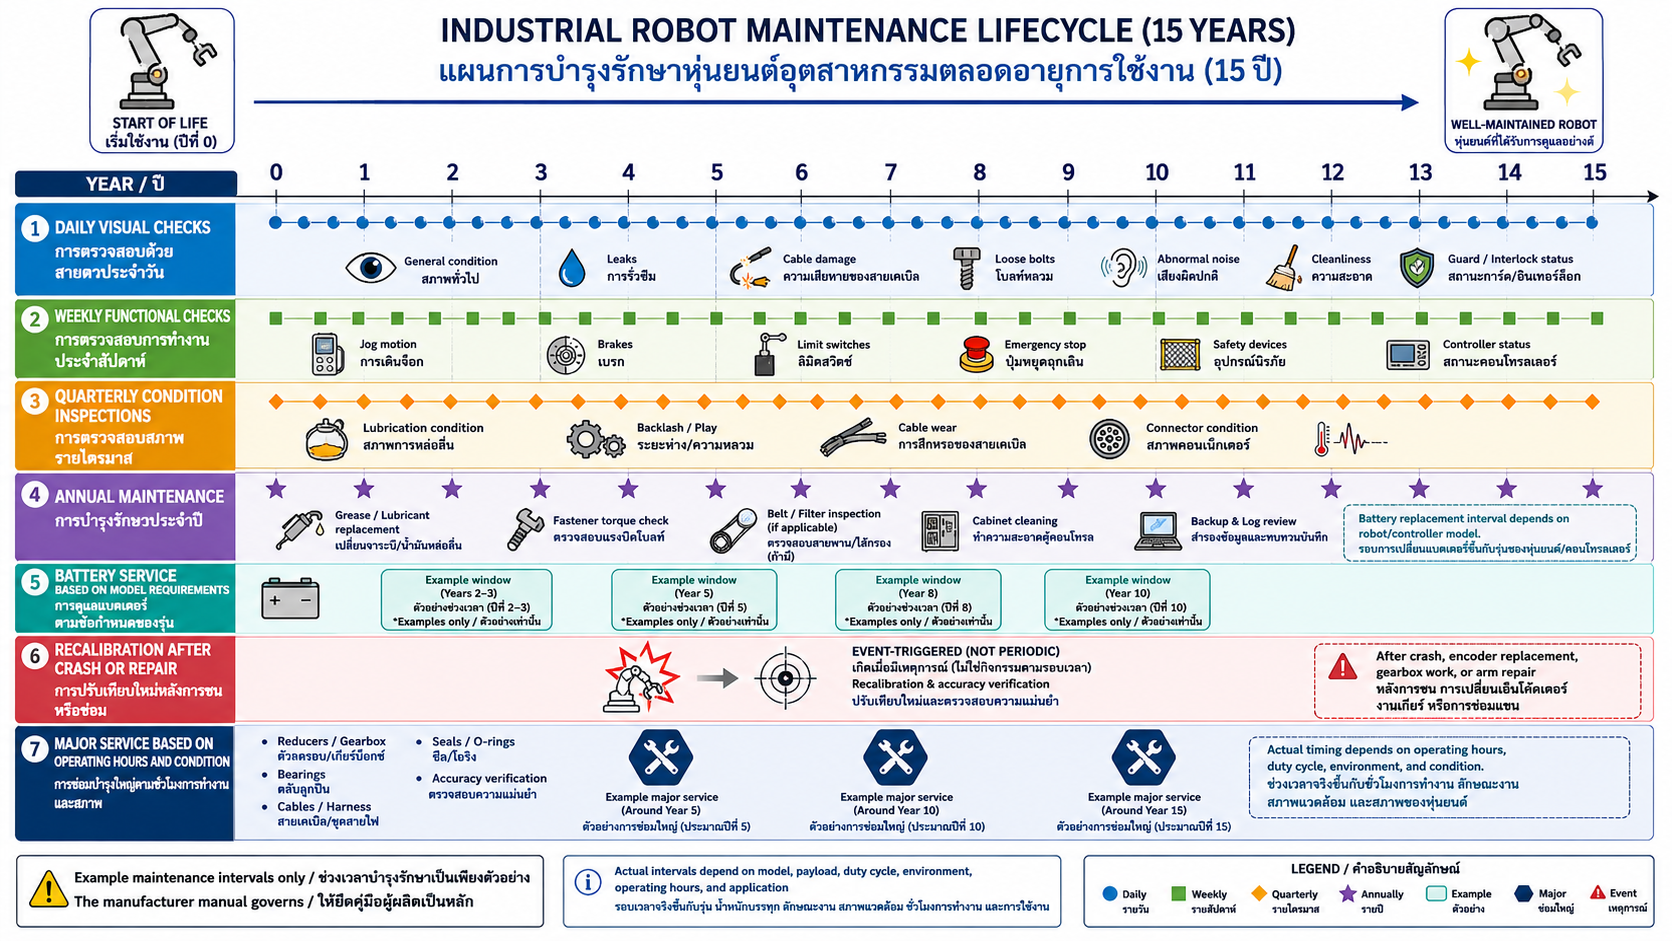
\includegraphics[width=0.8\textwidth]{images/chapter8/figure-04.png}
    \caption{แผน PM ตลอดวงจรชีวิตหุ่นยนต์}
\end{figure}

% [รูปที่ 8.5: Mastering Marks และการตั้งตำแหน่งอ้างอิง]
% ประเภทภาพ: Technical Illustration
% ตำแหน่งที่แนะนำ: หลังหัวข้อ 7.5.7
% วัตถุประสงค์การเรียนรู้: แสดงหลักการจัดแนว Mark ของ Joint ก่อนทำ Mastering
% คำอธิบายภาพ: ภาพระยะใกล้ของ Joint หุ่นยนต์ที่มี Witness Marks สองด้าน พร้อมลูกศรแสดงการจัดแนวและป้ายเตือนให้ใช้วิธีของผู้ผลิต
% องค์ประกอบที่ต้องมี: Joint housing, two alignment marks, axis direction, calibration tool placeholder, caution label
% ข้อความหรือป้ายกำกับ: Mastering Mark, Align per Product Manual, Do Not Estimate
% ภาษาของป้ายกำกับ: ไทยและอังกฤษ
% สัดส่วนภาพ: 16:9
% Image Generation Prompt: Close-up engineering textbook illustration of an industrial robot joint showing two mastering witness marks that must be aligned. Include axis direction arrow, a generic calibration tool reference, and a clear caution that the exact mastering procedure is model-specific and must follow the product manual. White background, realistic technical vector style, bilingual Thai-English labels, 16:9.
% Alt Text: รอย Mastering สองตำแหน่งบน Joint ที่ต้องจัดแนวตามคู่มือผู้ผลิต

\begin{figure}[htbp]
    \centering
    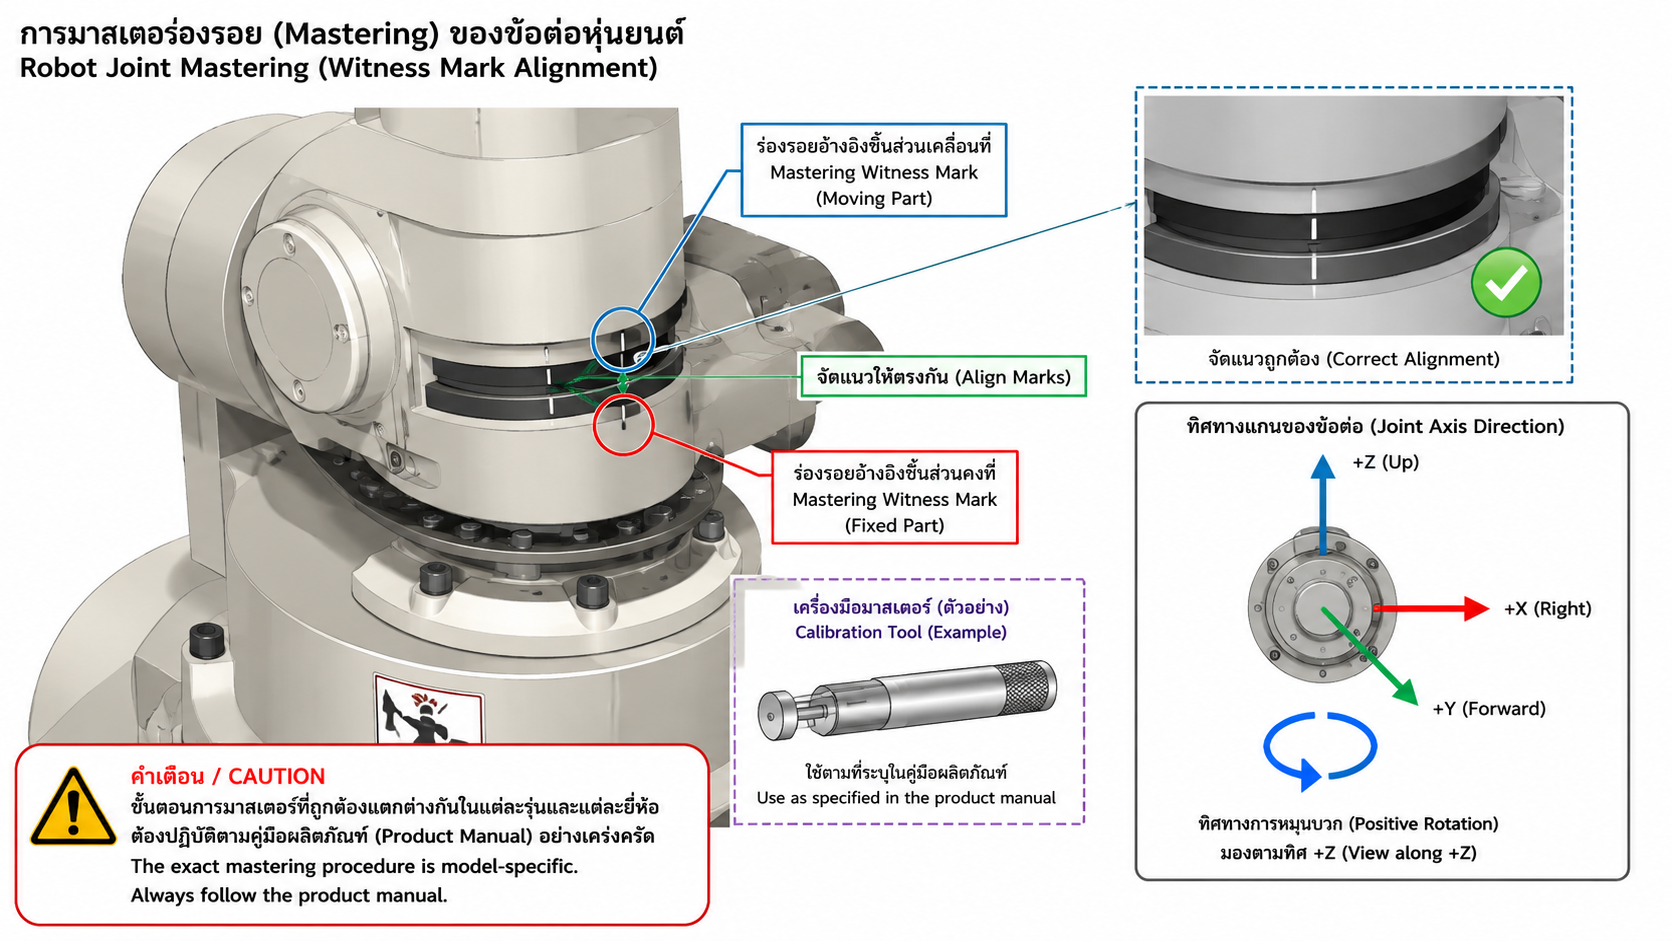
\includegraphics[width=0.8\textwidth]{images/chapter8/figure-05.png}
    \caption{Mastering Marks และการตั้งตำแหน่งอ้างอิง}
\end{figure}

\par\noindent\rule{\textwidth}{0.4pt}\par

\subsection{7.6 การแก้ไขปัญหาเบื้องต้น}

\subsubsection{7.6.1 หลักการ Troubleshooting}

Troubleshooting ที่มีประสิทธิภาพต้องแยก “อาการ” ออกจาก “สาเหตุ” ตัวอย่างเช่น หุ่นยนต์หยุดที่จุด Pick เป็นอาการ สาเหตุอาจเป็น Sensor ไม่มา Air Pressure ต่ำ โปรแกรมรอสัญญาณผิด Address Gripper จับไม่สำเร็จ หรือ Safety Stop จากอุปกรณ์อื่น การเปลี่ยน Parameter โดยยังไม่ระบุสาเหตุอาจทำให้ปัญหาซับซ้อนและสร้างความเสี่ยง

กระบวนการพื้นฐาน 6 ขั้น

\begin{enumerate}
    \item \textbf{สังเกตอาการ} — เกิดเมื่อใด จุดใด เกิดซ้ำหรือไม่ และเกิดหลังการเปลี่ยนแปลงใด
    \item \textbf{อ่านข้อมูลระบบ} — Alarm Code, Event Log, Program Line, I/O State และ Axis Data
    \item \textbf{ทำให้ระบบปลอดภัย} — หยุด Cycle แยกพลังงานเมื่อจำเป็น และห้าม Reset ซ้ำโดยไม่เข้าใจเงื่อนไข
    \item \textbf{สร้างสมมติฐาน} — จัดลำดับสาเหตุจากเป็นไปได้สูงและตรวจง่ายไปต่ำ
    \item \textbf{ทดสอบทีละส่วน} — เปลี่ยนตัวแปรครั้งละหนึ่งอย่างและบันทึกผล
    \item \textbf{ยืนยันและป้องกันซ้ำ} — ทดสอบหลาย Cycle คืนค่า Guard/Parameter บันทึก Root Cause และ Action
\end{enumerate}

\subsubsection{7.6.2 การจำแนกปัญหา}

\begin{table}[htbp]
    \centering
    \small
    \begin{tabularx}{\textwidth}{@{}L{0.20\textwidth}L{0.30\textwidth}Y@{}}
        \hline
        \textbf{กลุ่มปัญหา} & \textbf{ตัวอย่างอาการ} & \textbf{ข้อมูลที่ควรตรวจ} \\
        \hline
        Safety & Protective Stop, Gate Open, Chain Fault & Safety PLC, Gate Switch, E-stop, Scanner Zone, Reset Sequence \\
        Servo/Drive & Overcurrent, Overload, Overtemperature & Payload, Collision, Brake, Cable, Axis Load, Speed/Acceleration \\
        Position Feedback & Encoder Alarm, Position Lost & Encoder Cable, Battery, Connector, Mastering Status \\
        Mechanical & เสียง สั่น Backlash รั่ว & Gearbox, Bearing, Fastener, Tool, Dress Pack \\
        I/O/Peripheral & Wait ค้าง Gripper ไม่ตอบ & Input State, Output Voltage, Air/Vacuum, Sensor Alignment \\
        Program/Logic & Jump ผิด Loop ไม่จบ & Program Pointer, Register, Label, Timeout, Recipe \\
        Communication & PLC/Fieldbus Disconnect & Network Status, Node, Cable, Address, Watchdog \\
        Process & Weld Fault, Pick Fail, Quality Drift & Process Parameter, Consumable, Tool Wear, Part Tolerance \\
        \hline
    \end{tabularx}
\end{table}

\subsubsection{7.6.3 การอ่าน Alarm อย่างเป็นระบบ}

เมื่อพบ Alarm ควรบันทึก

\begin{itemize}
    \item วันและเวลา
    \item รหัสและข้อความเต็ม
    \item Program และ Line ที่เกิด
    \item Operating Mode
    \item ตำแหน่ง Joint/TCP
    \item I/O และ State ของอุปกรณ์
    \item Payload/Recipe ที่ใช้งาน
    \item การเปลี่ยนแปลงก่อนเกิด Alarm
    \item การดำเนินการที่ทำและผลลัพธ์
\end{itemize}

การ Reset Alarm โดยไม่บันทึกข้อมูลทำให้สูญเสียหลักฐานสำคัญและอาจทำให้ความผิดปกติเกิดซ้ำ

\subsubsection{ตาราง 8.6 ตัวอย่าง Alarm Code ตามขอบเขตที่กำหนด}

\begin{table}[htbp]
    \centering
    \small
    \begin{tabularx}{\textwidth}{@{}L{0.16\textwidth}L{0.28\textwidth}Y@{}}
        \hline
        \textbf{Error Code} & \textbf{ความหมายที่ใช้ในตัวอย่าง} & \textbf{แนวทางตรวจสอบเบื้องต้น} \\
        \hline
        SRVO-003 & Encoder Disconnect & ทำให้ระบบปลอดภัย ตรวจ Connector และสาย Feedback ตามคู่มือ \\
        SRVO-006 & Overcurrent & ตรวจการชน โหลด Brake สายมอเตอร์ และค่าความเร่ง ห้าม Reset ซ้ำต่อเนื่อง \\
        SRVO-012 & Overload & ตรวจ Payload, Center of Gravity, Duty Cycle และกลไกติดขัด \\
        SRVO-062 & Pulse/Position-related mismatch ตามตัวอย่าง & ตรวจข้อความ Alarm ฉบับเต็ม Battery และ Mastering Status ก่อนทำ Mastering \\
        SRVO-064 & Over-speed-related alarm ตามตัวอย่าง & ตรวจคำสั่ง Speed, Parameter, Feedback และสภาพกลไกตาม Manual \\
        SRVO-230 & Safety chain-related fault ตามตัวอย่าง & ตรวจ Safety Chain, Gate, E-stop และ Safety Hardware โดยผู้มีความสามารถ \\
        \hline
    \end{tabularx}
\end{table}

\begin{quote}
\textbf{ข้อจำกัดของตาราง:} รหัส Alarm และความหมายอาจแตกต่างตาม Controller Family, Software Option และ Revision ตารางนี้คงรายการตามขอบเขตบทเพื่อการฝึกวิเคราะห์เท่านั้น ก่อนปฏิบัติจริงต้องเปิด Alarm Code Manual ของ Controller และใช้ข้อความ Alarm เต็มจากหน้าจอเป็นแหล่งอ้างอิงหลัก
\end{quote}

\subsubsection{7.6.4 Fault Isolation}

การแยกสาเหตุควรเริ่มจากหลักฐาน ไม่ใช่การเปลี่ยนอะไหล่โดยคาดเดา ตัวอย่างกรณี Gripper ไม่ยืนยัน

\begin{verbatim}
อาการ: WAIT GRIP_OK ค้าง
    |-- Output GRIP_CLOSE ไม่ ON -> ตรวจ Program/Interlock/Output Module
    |-- Output ON แต่ Solenoid ไม่ทำงาน -> ตรวจแรงดัน สาย วาล์ว
    |-- Solenoid ทำงานแต่ Gripper ไม่ขยับ -> ตรวจ Air Pressure/กลไกติดขัด
    |-- Gripper ขยับแต่ Sensor ไม่ ON -> ตรวจตำแหน่ง Sensor/สาย/Input
    `-- Input ON ที่ Module แต่ Robot ไม่เห็น -> ตรวจ Mapping/Fieldbus
\end{verbatim}

การไล่ตามลำดับดังกล่าวลดการถอดอุปกรณ์โดยไม่จำเป็นและทำให้รายงาน Root Cause ชัดเจน

\subsubsection{7.6.5 Safe Recovery}

หลังแก้สาเหตุ ต้องวางแผน Recovery ตาม State ของระบบ

\begin{enumerate}
    \item ยืนยันว่าบุคลากรออกจากพื้นที่อันตราย
    \item คืน Guard, Connector และ Safety Device ครบ
    \item ตรวจว่าหุ่นยนต์ถือชิ้นงานหรือไม่
    \item ตรวจว่า Clamp, Machine Door, Conveyor และ Tool อยู่สถานะใด
    \item เลือก Recovery Routine หรือ Jog ไปยัง Safe Pose ที่กำหนด
    \item หลีกเลี่ยงการ Jump ข้ามคำสั่งที่ทำให้ I/O ไม่สอดคล้องกับสภาพจริง
    \item Reset Counter/State เฉพาะค่าที่จำเป็น
    \item Dry Run หนึ่ง Cycle ที่ความเร็วต่ำ
    \item จึงคืน Automatic Mode ตามขั้นตอนอนุมัติ
\end{enumerate}

% [รูปที่ 8.6: Flowchart การ Troubleshooting หุ่นยนต์]
% ประเภทภาพ: Flowchart
% ตำแหน่งที่แนะนำ: หลังหัวข้อ 7.6.1
% วัตถุประสงค์การเรียนรู้: แสดงลำดับสังเกต–ทำให้ปลอดภัย–วิเคราะห์–ทดสอบ–ยืนยัน
% คำอธิบายภาพ: เริ่มจาก Symptoms ไป Alarm/Log จากนั้น Safe State, Hypothesis, Test One Variable, Verify, Document และ Decision Loop กลับเมื่อยังไม่พบสาเหตุ
% องค์ประกอบที่ต้องมี: Start, Symptoms, Safety, Data Collection, Hypothesis, Test, Result, Verify, Record, Escalate
% ข้อความหรือป้ายกำกับ: Do not bypass safety, Change one variable at a time
% ภาษาของป้ายกำกับ: ไทยและอังกฤษ
% สัดส่วนภาพ: 16:9
% Image Generation Prompt: Systematic industrial robot troubleshooting flowchart: observe symptoms, read alarm and event logs, place system in a safe state, collect hardware and software evidence, form hypotheses, test one variable at a time, verify the repair, document root cause, and escalate when unresolved. Include decision loops and a warning not to bypass safety. Clean engineering textbook vector style, bilingual Thai-English labels, white background, 16:9.
% Alt Text: ผังงานการแก้ปัญหาจากอาการไปสู่การยืนยันและบันทึกสาเหตุ

\begin{figure}[htbp]
    \centering
    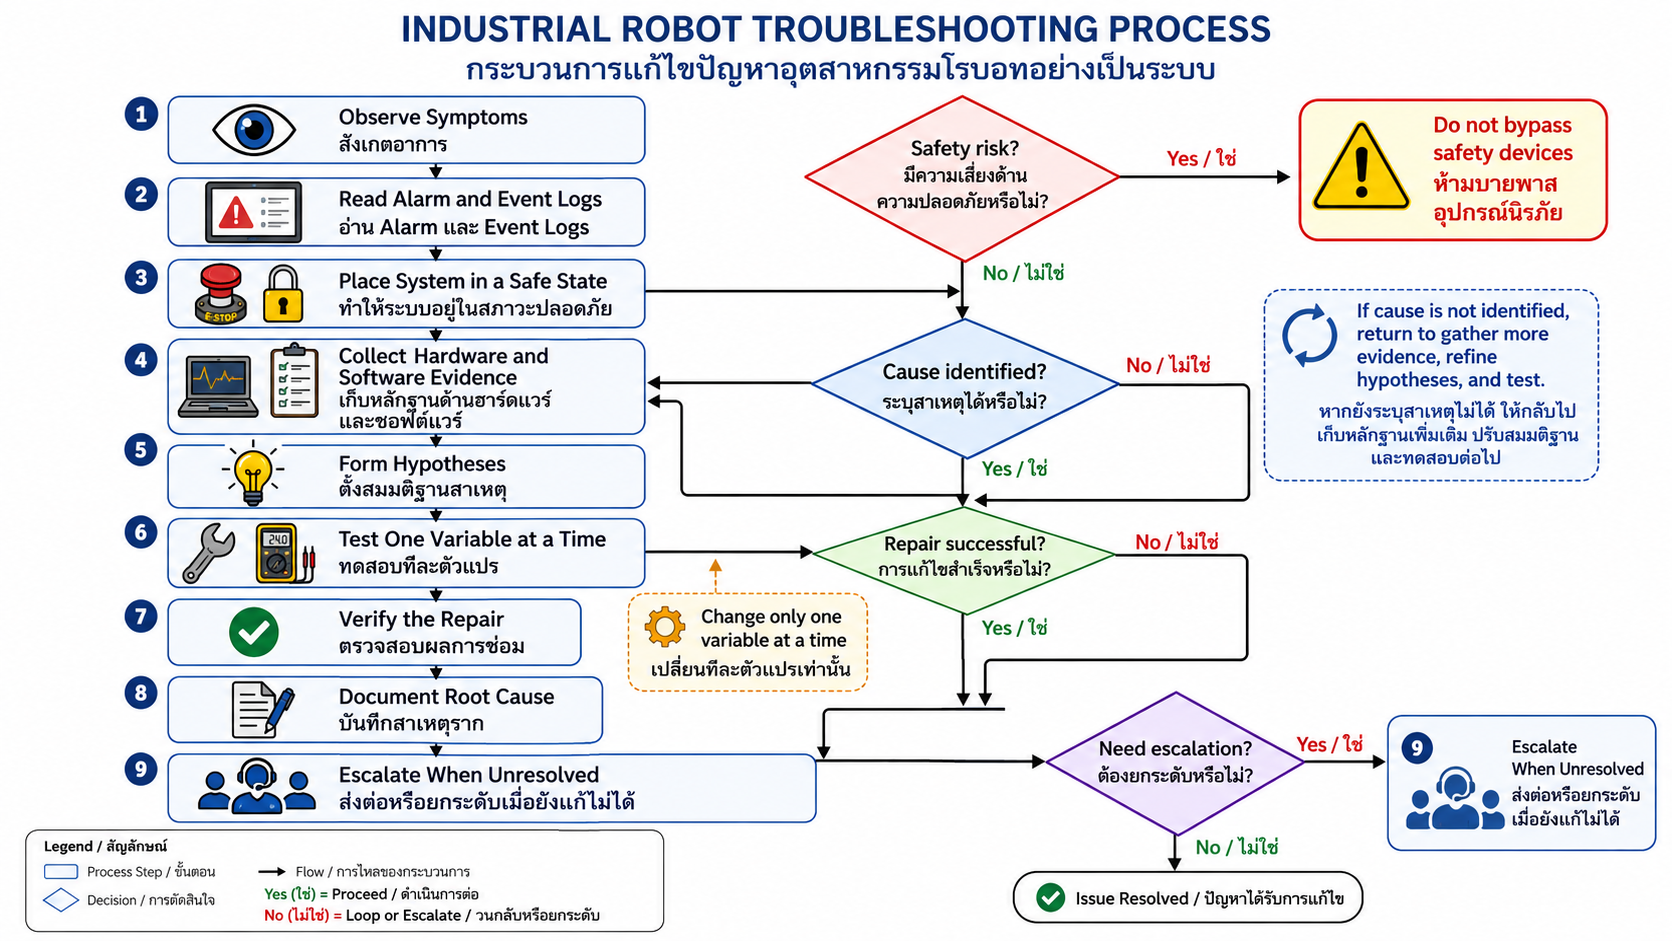
\includegraphics[width=0.8\textwidth]{images/chapter8/figure-06.png}
    \caption{Flowchart การ Troubleshooting หุ่นยนต์}
\end{figure}

\par\noindent\rule{\textwidth}{0.4pt}\par

\subsection{7.7 ความปลอดภัยในการทำงานกับหุ่นยนต์}

\subsubsection{7.7.1 กรอบมาตรฐานที่เกี่ยวข้อง}

การจัดการความปลอดภัยของหุ่นยนต์อุตสาหกรรมต้องพิจารณาทั้งตัวหุ่นยนต์และการรวมเป็นเซลล์

\begin{itemize}
    \item \textbf{ISO 10218-1:2025} ครอบคลุมข้อกำหนดด้านการออกแบบและการลดความเสี่ยงของ Industrial Robot
    \item \textbf{ISO 10218-2:2025} ครอบคลุม Robot Application, Integration, Commissioning, Operation และ Maintenance ของ Robot Cell
    \item \textbf{ISO 12100:2010} ให้หลัก Risk Assessment และ Risk Reduction ของเครื่องจักร
    \item \textbf{ISO 13855:2024} ใช้พิจารณาตำแหน่งและมิติของ Safeguard ตามการเข้าถึงของร่างกาย
    \item \textbf{ISO 13849-1:2023} ให้หลักการออกแบบ Safety-related Parts of Control Systems และ Performance Level
    \item \textbf{ISO 11161:2007/Amd 1:2010} ยังเป็นมาตรฐานปัจจุบันสำหรับ Integrated Manufacturing Systems ณ วันที่จัดทำเอกสาร แต่มีฉบับใหม่อยู่ระหว่างกระบวนการแทนที่
    \item \textbf{ข้อกำหนด LOTO ของสถานประกอบการและกฎหมายที่ใช้บังคับ} ต้องนำมาใช้กับงานซ่อมบำรุงและการควบคุมพลังงานอันตราย
\end{itemize}

การกล่าวว่า Safety PLC เป็น “SIL 2–3 หรือ PL d–e” โดยไม่ทำ Risk Assessment และ Validation ไม่เพียงพอ ระดับที่ต้องการต้องได้จากการประเมินความเสี่ยงและการออกแบบ Safety Function แต่ละฟังก์ชัน

\subsubsection{7.7.2 ลำดับชั้นการลดความเสี่ยง}

แนวทางตาม ISO 12100 เริ่มจาก

\begin{enumerate}
    \item \textbf{Inherently Safe Design:} ลดอันตรายด้วยการออกแบบ เช่น ลดขอบคม ลดแรง/ความเร็ว หรือจำกัดช่วงเคลื่อนที่
    \item \textbf{Safeguarding and Protective Measures:} รั้ว Interlock, Light Curtain, Scanner, Pressure Mat และ Safety Function
    \item \textbf{Information for Use:} Warning, Procedure, Training, PPE และ Sign
\end{enumerate}

PPE และป้ายเตือนไม่สามารถทดแทน Guard หรือการแยกพลังงานเมื่อยังมีอันตรายจากการเคลื่อนที่ของหุ่นยนต์

\subsubsection{7.7.3 Operating Modes และการสอน}

ระบบหุ่นยนต์อาจมี Automatic, Manual Reduced-speed และโหมดอื่นตามผู้ผลิต ในห้องปฏิบัติการควรกำหนดว่า

\begin{itemize}
    \item การสอนและ Touch-up ใช้ Manual Reduced-speed เท่านั้น
    \item ใช้ Enabling Device ตามการออกแบบของ Teach Pendant
    \item มีผู้ควบคุม Pendant คนเดียวและมีอำนาจหยุดการทดลอง
    \item ห้ามผู้เรียนอยู่ในพื้นที่พร้อมกันหลายคนโดยไม่มีบทบาทชัดเจน
    \item ห้ามใช้ Automatic เมื่อประตูเปิดหรือ Safeguard ถูก Bypass
    \item ค่า 250 mm/s มักพบเป็นขีดจำกัดอ้างอิงสำหรับการเคลื่อนที่แบบ Manual Reduced-speed ในระบบอุตสาหกรรมหลายชนิด แต่ต้องใช้ค่าที่มาตรฐานและผู้ผลิตกำหนดสำหรับระบบจริง ไม่ควรตั้งค่าโดยอาศัยตัวเลขนี้เพียงอย่างเดียว
\end{itemize}

\subsubsection{7.7.4 Safety Distance}

รูปแบบสมการพื้นฐานที่ใช้ในบทเรียนคือ

\[
S=K\times T+C
\]

เมื่อ

\begin{itemize}
    \item $S$ คือระยะต่ำสุดจาก Detection Zone ถึง Hazard Zone หน่วย mm
    \item $K$ คือความเร็วเข้าหาที่มาตรฐานกำหนด หน่วย mm/s
    \item $T$ คือ \textbf{เวลาตอบสนองรวมของระบบ} หน่วย s
    \item $C$ คือระยะเพิ่มที่สัมพันธ์กับการเข้าถึงหรือการทะลุผ่านอุปกรณ์ตรวจจับ หน่วย mm
\end{itemize}

เวลารวม $T$ ต้องรวมองค์ประกอบที่เกี่ยวข้อง เช่น

\[
T=T_{sensor}+T_{logic}+T_{network}+T_{machine\ stop}+T_{margin}
\]

การใช้เฉพาะ Response Time ของ Light Curtain โดยไม่รวมเวลาหยุดของหุ่นยนต์จะทำให้ระยะที่คำนวณต่ำเกินจริง

\subsubsection{ตัวอย่างที่ 8.5 การคำนวณระยะป้องกันตามข้อมูลโจทย์}

\textbf{ตัวอย่างเพิ่มเติมเพื่อการเรียนรู้}

กำหนด $K=2{,}000$ mm/s, $T=15$ ms และ $C=850$ mm โดยสมมติว่า 15 ms เป็นเวลารวมทั้งหมดตามโจทย์

แปลงหน่วย

\[
T=15\text{ ms}=0.015\text{ s}
\]

คำนวณ

\[
S=(2{,}000)(0.015)+850=30+850=880\text{ mm}
\]

ดังนั้นระยะต่ำสุดตามสมมติฐานของโจทย์คือ \textbf{880 mm}

\textbf{ข้อควรระวังในการออกแบบจริง:} หาก 15 ms เป็นเพียงเวลาของ Sensor ต้องวัดหรือใช้ค่า Stop Time รวมของ Robot Cell แล้วคำนวณใหม่ รวมทั้งตรวจสูตรและค่าคงที่สำหรับชนิดอุปกรณ์ตาม ISO 13855:2024 และคู่มือผู้ผลิต

\subsubsection{7.7.5 Warning Zone และ Protective Zone}

Area Scanner สามารถกำหนดหลาย Zone เช่น

\begin{itemize}
    \item \textbf{Warning Zone:} ตรวจพบบุคคลแล้วเตือน ลดความเร็ว หรือเตรียมหยุดตามการออกแบบ
    \item \textbf{Protective Zone:} การบุกรุกทำให้เกิด Protective Stop ที่ผ่านการออกแบบและ Validation
    \item \textbf{Restart Interlock:} ระบบต้องไม่เริ่มใหม่โดยอัตโนมัติเมื่อพื้นที่กลับมาว่าง หากยังมีความเป็นไปได้ว่าบุคคลอยู่ในพื้นที่อันตรายหรือเงื่อนไข Reset ไม่ครบ
\end{itemize}

การกำหนด Zone ต้องพิจารณา Stop Time, Scanner Resolution, Field Tolerance, Floor Reflection, Blind Spot, Tool Extension และตำแหน่งทุกแกน ไม่ใช่ดูเฉพาะฐานหุ่นยนต์

\subsubsection{7.7.6 LOTO สำหรับงานบำรุงรักษา}

ขั้นตอนทั่วไปของ LOTO

\begin{enumerate}
    \item แจ้งผู้เกี่ยวข้องและระบุขอบเขตงาน
    \item หยุดระบบด้วยวิธีปกติ
    \item ระบุแหล่งพลังงานทั้งหมด เช่น ไฟฟ้า Pneumatic, Hydraulic, Gravity, Spring และ Stored Energy
    \item แยกแหล่งพลังงานด้วย Disconnect/Valve ที่เหมาะสม
    \item ล็อกและติดป้ายโดยผู้ปฏิบัติงานแต่ละคน
    \item ระบายหรือควบคุม Stored Energy
    \item ยืนยัน Zero-energy State ตามวิธีที่กำหนด
    \item ดำเนินงาน
    \item ตรวจพื้นที่และประกอบ Guard/Connector กลับ
    \item นำ Lock ออกโดยผู้เป็นเจ้าของตาม Procedure
    \item แจ้งผู้เกี่ยวข้องและคืนระบบอย่างควบคุม
\end{enumerate}

การกด Hold, Cycle Stop หรือ Emergency Stop \textbf{ไม่เท่ากับ LOTO} เพราะพลังงานยังอาจคงอยู่และระบบอาจถูก Reset ได้

\subsubsection{7.7.7 ขั้นตอนก่อนเข้าสู่พื้นที่ Safeguarded Space}

\begin{verbatim}
1. หยุด Cycle ตามขั้นตอนที่อนุมัติ
2. ยืนยันสถานะหุ่นยนต์และอุปกรณ์รอบข้าง
3. เปิด Gate ผ่าน Interlock โดยไม่ Bypass
4. หากเป็นงานซ่อม/ปรับแต่งที่สัมผัสอันตราย ให้ทำ LOTO
5. หากเป็นงาน Teaching ที่ได้รับอนุญาต ใช้ Manual Reduced-speed และ Enabling Device
6. นำ Teach Pendant เข้าไปกับผู้ควบคุม ห้ามวางไว้นอกพื้นที่ให้ผู้อื่นสั่ง
7. ตรวจ Escape Path และ Pinch/Crush Zone
8. สื่อสารบทบาทของทุกคนก่อนเริ่มเคลื่อนที่
\end{verbatim}

% [รูปที่ 8.7: Warning Zone และ Protective Zone ของเซลล์หุ่นยนต์]
% ประเภทภาพ: Safety Zone Diagram
% ตำแหน่งที่แนะนำ: หลังหัวข้อ 7.7.5
% วัตถุประสงค์การเรียนรู้: แสดงความสัมพันธ์ของ Hazard Zone, Protective Zone, Warning Zone, Scanner และ Gate
% คำอธิบายภาพ: มุมมองด้านบนของเซลล์หุ่นยนต์ มีรั้ว ประตู Interlock Scanner Field สองระดับ และลูกศรระยะหยุด
% องค์ประกอบที่ต้องมี: Robot, swept area, fence, gate, light curtain or scanner, warning field, protective field, reset station outside zone
% ข้อความหรือป้ายกำกับ: Hazard Zone, Protective Zone, Warning Zone, Interlocked Gate, Manual Reset
% ภาษาของป้ายกำกับ: ไทยและอังกฤษ
% สัดส่วนภาพ: 16:9
% Image Generation Prompt: Top-view industrial robot cell safety diagram with a six-axis robot, swept hazard area, perimeter fence, interlocked gate, safety laser scanner, outer warning zone, inner protective zone, and a manual reset station located outside the safeguarded space with clear visibility. Show separation distance and stopping direction arrows. Clean engineering vector style, bilingual Thai-English labels, white background, 16:9.
% Alt Text: มุมมองด้านบนของเซลล์หุ่นยนต์ที่มีเขตเตือน เขตป้องกัน รั้ว ประตู และจุด Reset นอกพื้นที่

\begin{figure}[htbp]
    \centering
    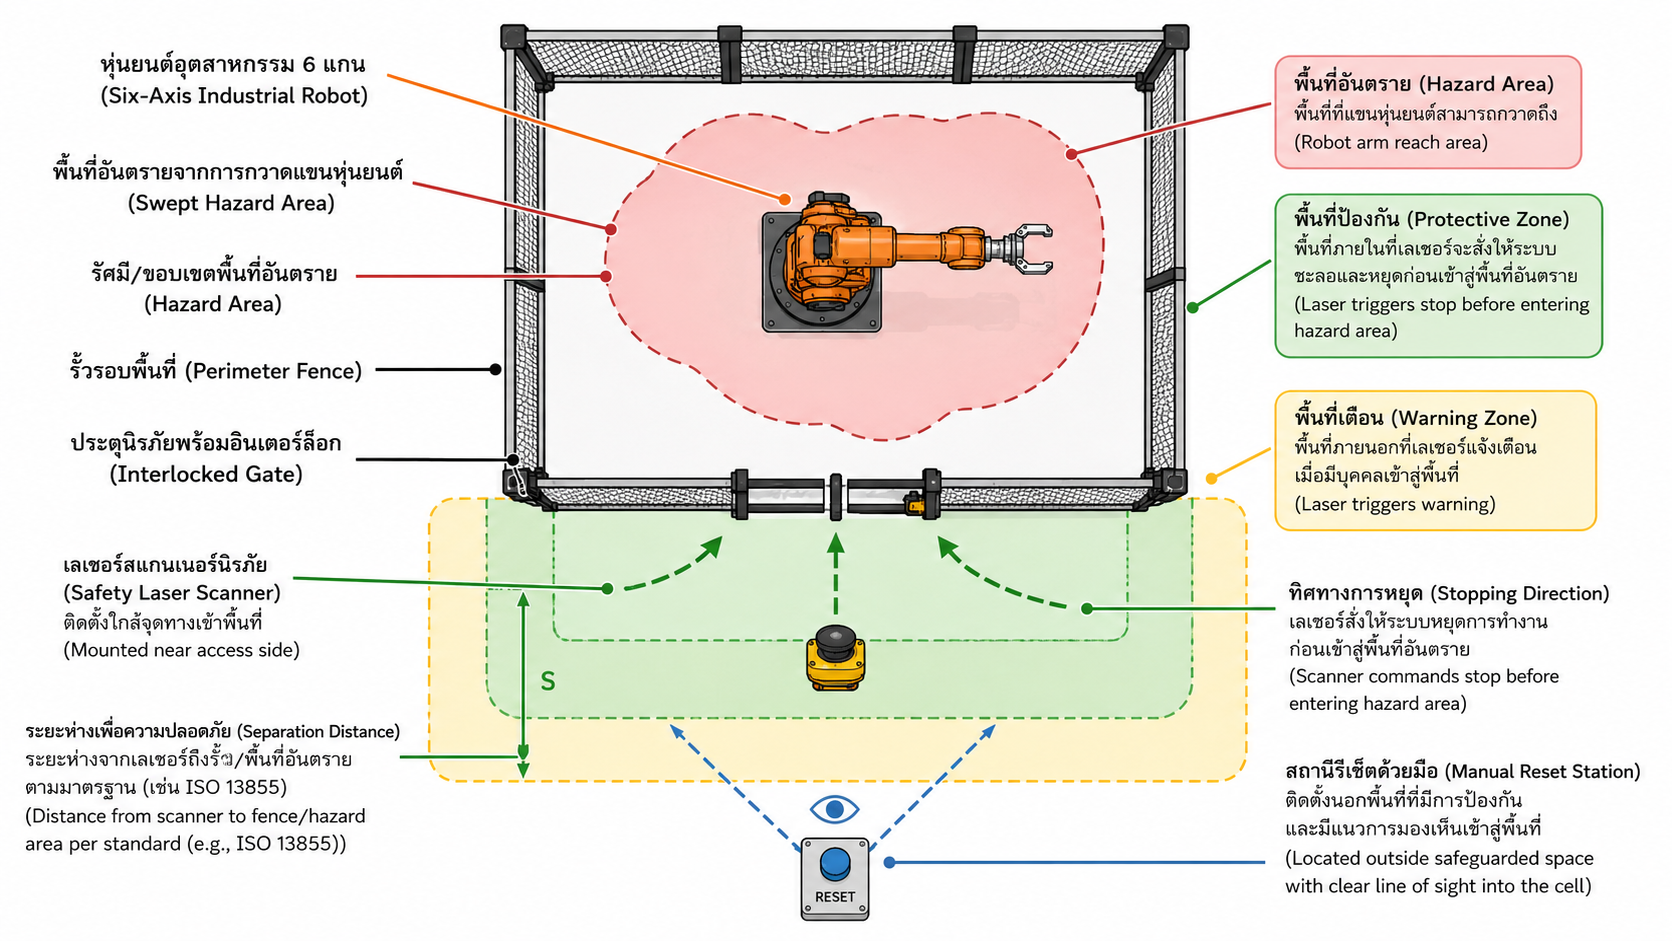
\includegraphics[width=0.8\textwidth]{images/chapter8/figure-07.png}
    \caption{Warning Zone และ Protective Zone ของเซลล์หุ่นยนต์}
\end{figure}

\par\noindent\rule{\textwidth}{0.4pt}\par

\subsection{7.8 เปรียบเทียบภาษาโปรแกรมและซอฟต์แวร์จากผู้ผลิต}

\subsubsection{ตาราง 8.7 ภาษาโปรแกรมหุ่นยนต์จากผู้ผลิตชั้นนำ}

\begin{table}[htbp]
    \centering
    \small
    \begin{tabularx}{\textwidth}{@{}L{0.13\textwidth}L{0.22\textwidth}L{0.17\textwidth}L{0.18\textwidth}Y@{}}
        \hline
        \textbf{ผู้ผลิต} & \textbf{ภาษา/สภาพแวดล้อม} & \textbf{Extension ตัวอย่าง} & \textbf{คำสั่งเคลื่อนที่หลัก} & \textbf{ซอฟต์แวร์ Offline/Simulation} \\
        \hline
        FANUC & TP Language / KAREL & \texttt{.LS}, \texttt{.TP}, \texttt{.KL} & \texttt{J}, \texttt{L}, \texttt{C} & ROBOGUIDE \\
        ABB & RAPID & \texttt{.MOD} & \texttt{MoveJ}, \texttt{MoveL}, \texttt{MoveC} & RobotStudio \\
        KUKA & KRL & \texttt{.SRC}, \texttt{.DAT} & \texttt{PTP}, \texttt{LIN}, \texttt{CIRC} & KUKA.Sim หรือแพลตฟอร์มวิศวกรรมที่รองรับรุ่นนั้น \\
        Yaskawa & INFORM & \texttt{.JBI} & \texttt{MOVJ}, \texttt{MOVL}, \texttt{MOVC} & MotoSim EG-VRC \\
        Mitsubishi & MELFA-BASIC & \texttt{.MB5} หรือรูปแบบตาม Controller & \texttt{MOV}, \texttt{MVS}, \texttt{MVR} & RT ToolBox3 \\
        Universal Robots & PolyScope / URScript & \texttt{.URP}, \texttt{.script} & \texttt{movej}, \texttt{movel}, \texttt{movec} & URSim/PolyScope Simulation \\
        \hline
    \end{tabularx}
\end{table}

ตารางนี้ใช้เพื่อเปรียบเทียบแนวคิด ไม่ควรสรุปว่าคำสั่งต่างยี่ห้อมีพฤติกรรมเหมือนกันทุกประการ ความหมายของ Speed, Zone, Orientation Interpolation, Configuration และ Error Handling ต่างกันตามระบบ

\subsubsection{ตาราง 8.8 แนวคิดที่เทียบเคียงข้ามผู้ผลิต}

\begin{table}[htbp]
    \centering
    \small
    \begin{tabularx}{\textwidth}{@{}L{0.22\textwidth}L{0.14\textwidth}L{0.17\textwidth}L{0.22\textwidth}Y@{}}
        \hline
        \textbf{แนวคิด} & \textbf{FANUC} & \textbf{ABB} & \textbf{KUKA} & \textbf{Universal Robots} \\
        \hline
        Joint Motion & \texttt{J} & \texttt{MoveJ} & \texttt{PTP} & \texttt{movej} \\
        Linear TCP Motion & \texttt{L} & \texttt{MoveL} & \texttt{LIN} & \texttt{movel} \\
        Circular TCP Motion & \texttt{C} & \texttt{MoveC} & \texttt{CIRC} & \texttt{movec} \\
        Exact Stop & \texttt{FINE} & \texttt{fine} & Approximation off/exact target & Blend radius \texttt{r=0} โดยแนวคิด \\
        Blending & \texttt{CNT} & \texttt{z10}, \texttt{z50}, ... & \texttt{\$APO}/Approximation & Blend radius \texttt{r} \\
        User Frame & \texttt{UFRAME} & \texttt{wobjdata} & Base & Feature/Plane \\
        Tool Frame & \texttt{UTOOL} & \texttt{tooldata} & Tool & TCP \\
        \hline
    \end{tabularx}
\end{table}

\par\noindent\rule{\textwidth}{0.4pt}\par

\subsection{7.9 กิจกรรมปฏิบัติการประจำบท}

\subsection{กิจกรรมปฏิบัติการที่ 8-1: การสอนตำแหน่งและเขียนโปรแกรม Pick-and-Place}

\subsubsection{1. วัตถุประสงค์}

เมื่อจบกิจกรรม นักศึกษาสามารถ

\begin{itemize}
    \item เลือก Joint, World, Tool และ User Coordinate ในการ Jog ได้เหมาะสม
    \item สอน Home, Approach, Pick, Place และ Retreat Point ได้
    \item เขียนโปรแกรม Motion, Gripper I/O, Wait และ Timeout ได้
    \item เปรียบเทียบผลของ Fine กับ Blending ต่อ Path และ Cycle Time ได้
    \item ปฏิบัติงานใน Manual Reduced-speed โดยใช้ Enabling Device ได้ถูกต้อง
\end{itemize}

\subsubsection{2. หลักการและทฤษฎีที่เกี่ยวข้อง}

กิจกรรมใช้หลัก Coordinate Frame, TCP, Approach–Process–Retreat, PTP/Linear Motion, Digital I/O และ Handshake โปรแกรมต้องแยกจุด Approach ออกจากจุด Pick/Place และต้องรอสัญญาณ Gripper Confirm ก่อนยกชิ้นงาน

\subsubsection{3. อุปกรณ์ เครื่องมือ และซอฟต์แวร์}

\begin{table}[htbp]
    \centering
    \begin{tabular}{l r l}
        \hline
        \textbf{รายการ} & \textbf{จำนวน} & \textbf{ข้อกำหนด} \\
        \hline
        ชุดหุ่นยนต์เพื่อการศึกษา & 1 ชุด/กลุ่ม & มี Teach Pendant, Guard และ Manual Mode \\
        Gripper ที่ติดตั้งและตรวจสอบแล้ว & 1 ชุด & ใช้แรง/แรงดันตามระบบฝึก \\
        ชิ้นงานจำลองน้ำหนักเบา & 3–5 ชิ้น & ไม่มีขอบคม แตกง่าย หรืออันตราย \\
        ถาด Pick และ Place & อย่างละ 1 & ยึดกับโต๊ะหรือ Fixture \\
        Checklist ความปลอดภัย & 1 ชุด/กลุ่ม & ใช้ก่อนเปิด Motion \\
        Stopwatch/Controller Cycle Timer & 1 & ใช้วัดเวลาเทียบ \\
        ซอฟต์แวร์จำลอง ถ้ามี & 1 License/กลุ่ม & ใช้ตรวจเส้นทางก่อนหุ่นยนต์จริง \\
        \hline
    \end{tabular}
\end{table}

\subsubsection{4. แผนภาพหรือชุดทดลอง}

\begin{verbatim}
Pick Tray -> P_PICK_APP -> P_PICK
                         |  Gripper Close + Confirm
P_PLACE_APP -> P_PLACE -> Place Tray
                         |  Gripper Open + Confirm
Return -> P_HOME
\end{verbatim}

\subsubsection{5. ข้อควรระวังด้านความปลอดภัย}

\begin{itemize}
    \item ผู้ควบคุม Teach Pendant มีเพียงคนเดียวต่อรอบ
    \item เริ่มจาก Simulation หรือ Robot ไม่มีชิ้นงาน
    \item ใช้ Manual Reduced-speed และ Step/Single Block
    \item ห้ามเข้า Automatic ขณะ Gate เปิด
    \item ห้ามจับแขนหรือ End Effector ของหุ่นยนต์อุตสาหกรรมทั่วไปด้วยมือ
    \item ห้าม Bypass Gripper Sensor หรือ Safety Interlock เพื่อให้กิจกรรมผ่าน
    \item หากมีการเคลื่อนที่ผิดทิศ ให้ปล่อย Enabling Device หรือใช้วิธีหยุดที่ได้รับการฝึกทันที
\end{itemize}

\subsubsection{6. ขั้นตอนการปฏิบัติ}

\begin{enumerate}
    \item ทำ Pre-job Briefing และตรวจ Checklist ความปลอดภัย
    \item เปิดระบบตาม Standard Operating Procedure ของห้องปฏิบัติการ
    \item เลือก Tool Frame และ User Frame ที่อาจารย์กำหนด
    \item ตรวจ TCP ด้วยจุดอ้างอิงโดยไม่ชนหรือกด Tool ลงบน Jig
    \item Jog ด้วย Joint Coordinate ไปยัง \texttt{P\_HOME}
    \item ใช้ World Coordinate ไปยังบริเวณเหนือ Pick Fixture
    \item ใช้ Tool/User Coordinate สอน \texttt{P\_PICK\_APP} และ \texttt{P\_PICK}
    \item สอน \texttt{P\_PLACE\_APP} และ \texttt{P\_PLACE}
    \item เขียนโปรแกรมเริ่มต้นโดยใช้ Fine ทุกจุด
    \item เพิ่ม Gripper Close/Open และ Wait Confirm พร้อม Timeout
    \item ตรวจโปรแกรมด้วย Static Review
    \item ทดสอบแบบ Step โดยไม่ใช้ชิ้นงาน
    \item ทดสอบด้วยชิ้นงานจำลองเมื่ออาจารย์อนุญาต
    \item วัด Cycle Time จำนวน 3 รอบ
    \item เปลี่ยนเฉพาะจุดผ่านกลางอากาศเป็น Blend ระดับต่ำหรือกลาง
    \item ทดสอบ Path และ Clearance อีกครั้ง
    \item วัด Cycle Time 3 รอบและเปรียบเทียบ
    \item Backup โปรแกรมและส่ง Point List
\end{enumerate}

\subsubsection{7. ตารางบันทึกผล}

\begin{table}[htbp]
    \centering
    \begin{tabular}{l l l r l l l}
        \hline
        \textbf{จุด} & \textbf{Coordinate ที่ใช้สอน} & \textbf{Motion} & \textbf{Speed} & \textbf{Fine/Blend} & \textbf{Tool/User No.} & \textbf{ผลการตรวจ Clearance} \\
        \hline
        HOME &  &  &  &  &  &  \\
        PICK\_APP &  &  &  &  &  &  \\
        PICK &  &  &  &  &  &  \\
        PLACE\_APP &  &  &  &  &  &  \\
        PLACE &  &  &  &  &  &  \\
        \hline
    \end{tabular}
\end{table}

\begin{table}[htbp]
    \centering
    \begin{tabular}{l r r r r l}
        \hline
        \textbf{การทดลอง} & \textbf{Cycle 1 (s)} & \textbf{Cycle 2 (s)} & \textbf{Cycle 3 (s)} & \textbf{ค่าเฉลี่ย (s)} & \textbf{หมายเหตุ} \\
        \hline
        Fine ทุกจุด &  &  &  &  &  \\
        Blend เฉพาะจุดผ่าน &  &  &  &  &  \\
        \hline
    \end{tabular}
\end{table}

\subsubsection{8. การคำนวณและวิเคราะห์ผล}

ค่าเฉลี่ย Cycle Time

\[
\bar{t}=\frac{t_1+t_2+t_3}{3}
\]

ร้อยละการลด Cycle Time

\[
\%\text{Reduction}=\frac{\bar{t}_{Fine}-\bar{t}_{Blend}}{\bar{t}_{Fine}}\times100
\]

นักศึกษาต้องอธิบายว่าการลดเวลามาจากจุดใด และ Path Deviation ที่เพิ่มขึ้นยังอยู่ใน Clearance ที่ยอมรับได้หรือไม่

\subsubsection{9. การเปรียบเทียบผลจริงกับทฤษฎีหรือแบบจำลอง}

หากใช้ OLP ให้เปรียบเทียบ Cycle Time และ Path จาก Simulation กับระบบจริง พร้อมอธิบายความต่างจาก Acceleration Limit, Controller Option, Payload, I/O Delay และ Gripper Response

\subsubsection{10. คำถามหลังการทดลอง}

\begin{enumerate}
    \item เหตุใดจุด Pick และ Place จึงควรใช้ Fine มากกว่าจุดผ่านกลางอากาศ
    \item หากเปลี่ยน User Frame แล้วไม่สอนจุดใหม่ จุดทั้งหมดควรเปลี่ยนอย่างไร
    \item หาก \texttt{GRIP\_OK} ไม่มา โปรแกรมควรหยุดที่ State ใด
    \item จุดใดควรใช้ Linear Motion และเหตุใด
    \item Blending ที่มากเกินไปอาจทำให้เกิดความเสี่ยงใด
\end{enumerate}

\subsubsection{11. เกณฑ์การประเมิน}

\begin{table}[htbp]
    \centering
    \begin{tabular}{l r}
        \hline
        \textbf{เกณฑ์} & \textbf{คะแนน} \\
        \hline
        ความปลอดภัยและการใช้ Teach Pendant & 25 \\
        ความถูกต้องของ Tool/User Frame และ Point & 20 \\
        โปรแกรม Motion, I/O, Timeout & 25 \\
        การวัดและวิเคราะห์ Cycle Time & 15 \\
        การตั้งชื่อ Comment และ Backup & 10 \\
        การตอบคำถามหลังทดลอง & 5 \\
        \textbf{รวม} & \textbf{100} \\
        \hline
    \end{tabular}
\end{table}

\par\noindent\rule{\textwidth}{0.4pt}\par

\subsection{กิจกรรมปฏิบัติการที่ 8-2: Daily Check และการจัดทำแผน Preventive Maintenance}

\subsubsection{1. วัตถุประสงค์}

\begin{itemize}
    \item ตรวจสภาพภายนอกของหุ่นยนต์และ End Effector ได้อย่างเป็นระบบ
    \item แยก Normal Condition, Observation และ Defect ได้
    \item จัดทำ PM Schedule ตาม Manual-based, Time-based และ Condition-based ได้
    \item บันทึกหลักฐานโดยไม่แต่งค่าที่ไม่ได้วัด
\end{itemize}

\subsubsection{2. หลักการและทฤษฎีที่เกี่ยวข้อง}

PM ใช้การตรวจซ้ำตามรอบและเกณฑ์ที่กำหนด การสังเกตต้องอ้างอิง Baseline หรือคู่มือ ไม่ควรสรุปสาเหตุจากลักษณะภายนอกเพียงอย่างเดียว

\subsubsection{3. อุปกรณ์ เครื่องมือ และซอฟต์แวร์}

\begin{table}[htbp]
    \centering
    \begin{tabular}{l r l}
        \hline
        \textbf{รายการ} & \textbf{จำนวน} & \textbf{ข้อกำหนด} \\
        \hline
        หุ่นยนต์ที่หยุดและจัดสภาพปลอดภัย & 1 ชุด & ไม่อนุญาต Motion ระหว่าง Visual Check \\
        ไฟฉายแรงดันต่ำ & 1 & ใช้ส่องตรวจ ไม่สอดมือเข้า Pinch Point \\
        กระจกตรวจ & 1 & ด้ามยาว ไม่มีขอบคม \\
        Torque Mark Reference & 1 ชุด & ใช้สังเกต ไม่ขันจริงหากไม่มีค่าคู่มือ \\
        แบบฟอร์ม Daily/PM Record & 1 ชุด/กลุ่ม & มีช่องผู้ตรวจและหลักฐาน \\
        กล้องถ่ายภาพของหน่วยงาน & 1 & ไม่ถ่ายข้อมูลลับหรือ Serial ตามนโยบาย \\
        Product Manual ของรุ่นฝึก & 1 & ใช้หาค่ารอบและข้อกำหนด \\
        \hline
    \end{tabular}
\end{table}

\subsubsection{4. แผนภาพหรือวงจร}

ใช้รูปที่ 8.4 และแผนผังตำแหน่งตรวจของหุ่นยนต์รุ่นที่ห้องปฏิบัติการใช้งาน

\subsubsection{5. ข้อควรระวังด้านความปลอดภัย}

\begin{itemize}
    \item หยุดระบบและใช้วิธีแยกพลังงานตามขอบเขตงาน
    \item ไม่เปิด Cover หรือถอด Connector ในกิจกรรมพื้นฐาน
    \item ไม่เติม Grease ไม่ขัน Bolt และไม่เปลี่ยน Battery หากไม่มีคู่มือ เครื่องมือ และผู้ควบคุมที่ได้รับอนุญาต
    \item ห้ามยืนใต้ Payload หรือส่วนที่อาจตกจากแรงโน้มถ่วง
    \item ไม่ใช้มือสัมผัสบริเวณที่สงสัยว่าร้อนหรือมีรอยรั่ว
\end{itemize}

\subsubsection{6. ขั้นตอนการปฏิบัติ}

\begin{enumerate}
    \item อ่าน Manual หัวข้อ Maintenance Schedule ของรุ่นฝึก
    \item ระบุจุดตรวจรอบ Robot Base, Arm, Wrist, Tool และ Dress Pack
    \item ตรวจรอยรั่ว รอยแตก รอยขูด การบิดสาย และ Fastener Mark
    \item ตรวจ End Effector, Air Hose, Sensor และ Fixture
    \item ตรวจ Fan/Filter หรือ Controller Cabinet เฉพาะจุดที่อนุญาต
    \item ตรวจประวัติ Alarm และ PM ครั้งก่อนจากข้อมูลตัวอย่าง
    \item จัดประเภทผลเป็น \texttt{OK}, \texttt{Monitor}, \texttt{Action Required}, \texttt{Not Inspected}
    \item จัดทำแผน PM 1 ปี โดยอ้าง Manual และเพิ่ม Condition Check ที่เหมาะสม
    \item เสนอผู้รับผิดชอบและหลักฐานของแต่ละงาน
    \item นำเสนอ 5 นาทีต่อกลุ่ม
\end{enumerate}

\subsubsection{7. ตารางบันทึกผล}

\begin{table}[htbp]
    \centering
    \begin{tabular}{l l l l l l}
        \hline
        \textbf{จุดตรวจ} & \textbf{สภาพที่คาดหวัง} & \textbf{ผลตรวจ} & \textbf{หลักฐาน/ภาพ} & \textbf{ระดับ} & \textbf{การดำเนินการ} \\
        \hline
        Robot Base & ไม่มีการคลาย/รอยเคลื่อน &  &  &  &  \\
        Axis 1–3 & ไม่มีรอยรั่วหรือเสียงผิดปกติที่รายงาน &  &  &  &  \\
        Wrist Axis 4–6 & Cable ไม่บิดและ Cover สมบูรณ์ &  &  &  &  \\
        Dress Pack & ไม่มีรอยขูด หักพับ หรือตึง &  &  &  &  \\
        End Effector & Fastener/Sensor/Hose สมบูรณ์ &  &  &  &  \\
        Controller & Indicator/Fan/Filter ตามข้อกำหนด &  &  &  &  \\
        Safety Device & สถานะตาม Functional Test Procedure &  &  &  &  \\
        \hline
    \end{tabular}
\end{table}

\subsubsection{8. การคำนวณและวิเคราะห์ผล}

ให้นักศึกษาสร้าง Priority Number เชิงการศึกษา

\[
P=S\times O\times D
\]

โดย $S$ คือความรุนแรง $O$ คือโอกาสเกิด และ $D$ คือความยากในการตรวจพบ ให้คะแนน 1–5 ตัวชี้วัดนี้ใช้จัดลำดับการติดตามในกิจกรรมเท่านั้น ไม่แทน Risk Assessment ตามมาตรฐาน

\subsubsection{9. การเปรียบเทียบผลจริงกับทฤษฎีหรือแบบจำลอง}

เปรียบเทียบ PM Schedule ที่กลุ่มสร้างกับคู่มือผู้ผลิต ระบุรายการที่เป็น Mandatory, Recommended และ Condition-based เพิ่มเติม

\subsubsection{10. คำถามหลังการทดลอง}

\begin{enumerate}
    \item เหตุใดรอบ PM จึงไม่ควรคัดลอกจากหุ่นยนต์คนละรุ่น
    \item รอย Grease ใดควรจัดเป็น Monitor และข้อมูลใดต้องเก็บเพิ่ม
    \item หาก Torque Mark เลื่อน ควรทำอย่างไรก่อนขัน
    \item ประวัติ Alarm ช่วยวางแผน PM อย่างไร
    \item หลักฐานใดทำให้ PM Record ตรวจสอบย้อนหลังได้
\end{enumerate}

\subsubsection{11. เกณฑ์การประเมิน}

\begin{table}[htbp]
    \centering
    \begin{tabular}{l r}
        \hline
        \textbf{เกณฑ์} & \textbf{คะแนน} \\
        \hline
        ปฏิบัติตาม Safety Boundary & 25 \\
        ความครบถ้วนของ Visual Check & 20 \\
        การใช้คู่มือและไม่คาดเดาค่า & 20 \\
        คุณภาพ PM Schedule & 20 \\
        หลักฐานและการสื่อสาร & 15 \\
        \textbf{รวม} & \textbf{100} \\
        \hline
    \end{tabular}
\end{table}

\par\noindent\rule{\textwidth}{0.4pt}\par

\subsection{กิจกรรมปฏิบัติการที่ 8-3: การอ่าน Alarm และ Troubleshooting ด้วยสถานการณ์จำลอง}

\subsubsection{1. วัตถุประสงค์}

\begin{itemize}
    \item อ่าน Alarm Code, Event Log, Program Line และ I/O State ได้
    \item สร้างแผน Fault Isolation ที่ตรวจทีละตัวแปรได้
    \item เลือก Safe Recovery และบันทึก Root Cause ได้
    \item แยกการ Reset, Repair, Mastering และ Escalation ได้
\end{itemize}

\subsubsection{2. หลักการและทฤษฎีที่เกี่ยวข้อง}

ใช้กระบวนการ Symptoms \(\rightarrow\) Safe State \(\rightarrow\) Evidence \(\rightarrow\) Hypothesis \(\rightarrow\) Test \(\rightarrow\) Verify \(\rightarrow\) Record การทดลองนี้มุ่งฝึกวิเคราะห์ ไม่มุ่งสร้าง Fault ทางกายภาพที่อาจทำให้อุปกรณ์เสียหาย

\subsubsection{3. อุปกรณ์ เครื่องมือ และซอฟต์แวร์}

\begin{table}[htbp]
    \centering
    \begin{tabular}{l r l}
        \hline
        \textbf{รายการ} & \textbf{จำนวน} & \textbf{ข้อกำหนด} \\
        \hline
        Robot Simulator หรือ Virtual Controller & 1 ชุด/กลุ่ม & ใช้ Fault/Alarm ที่ซอฟต์แวร์รองรับ \\
        ชุด I/O Trainer แรงดันต่ำ & 1 ชุด & ใช้จำลอง Sensor ON/OFF อย่างปลอดภัย \\
        Alarm Screenshot/Log ที่อาจารย์เตรียม & 3–5 กรณี & ลบข้อมูลลับและระบุ Controller Version \\
        Troubleshooting Worksheet & 1 ชุด/กลุ่ม & มีช่อง Evidence และ Test Result \\
        Multimeter & ตามความจำเป็น & ใช้เฉพาะวงจรฝึกแรงดันต่ำและภายใต้การกำกับ \\
        \hline
    \end{tabular}
\end{table}

\subsubsection{4. แผนภาพหรือวงจร}

ใช้รูปที่ 8.7 และ Block Diagram I/O Trainer

\subsubsection{5. ข้อควรระวังด้านความปลอดภัย}

\begin{itemize}
    \item \textbf{ห้ามถอด Encoder Connector ของหุ่นยนต์จริงขณะมีพลังงาน}
    \item \textbf{ห้ามเพิ่ม Payload เกิน Specification เพื่อสร้าง Overload Alarm}
    \item ใช้ Simulation, Alarm Log หรือ Fault Injection ที่ผู้ผลิต/อาจารย์กำหนด
    \item ไม่เปลี่ยน Safety Parameter, Servo Parameter หรือ Mastering Data เพื่อการทดลอง
    \item การวัดไฟฟ้าทำเฉพาะชุดฝึกแรงดันต่ำที่แยกจากวงจรหุ่นยนต์จริง
\end{itemize}

\subsubsection{6. ขั้นตอนการปฏิบัติ}

\begin{enumerate}
    \item รับ Case File จากอาจารย์ เช่น Gripper Timeout, Fieldbus Disconnect หรือ Position-related Alarm Log
    \item บันทึก Symptoms และข้อมูลที่มี
    \item ระบุอันตรายและวิธีทำให้ระบบปลอดภัย
    \item แยกสาเหตุที่เป็นไปได้อย่างน้อย 3 ข้อ
    \item จัดลำดับ Test จากไม่รบกวนระบบและมีความเสี่ยงต่ำ
    \item ตรวจ I/O, Program, Log หรือ Simulation ตาม Case
    \item บันทึกผลการทดสอบทุกขั้น
    \item ระบุ Root Cause หรือระดับความเชื่อมั่น
    \item เสนอ Corrective Action และ Preventive Action
    \item เขียน Safe Recovery Sequence
    \item แลก Case กับอีกกลุ่มเพื่อตรวจทาน
\end{enumerate}

\subsubsection{7. ตารางบันทึกผล}

\begin{table}[htbp]
    \centering
    \begin{tabular}{r l l l l l}
        \hline
        \textbf{ลำดับ} & \textbf{Evidence/อาการ} & \textbf{สมมติฐาน} & \textbf{วิธีทดสอบ} & \textbf{ผลทดสอบ} & \textbf{สรุป} \\
        \hline
        1 &  &  &  &  &  \\
        2 &  &  &  &  &  \\
        3 &  &  &  &  &  \\
        4 &  &  &  &  &  \\
        \hline
    \end{tabular}
\end{table}

\begin{table}[htbp]
    \centering
    \begin{tabular}{l l l l l}
        \hline
        \textbf{Root Cause} & \textbf{Corrective Action} & \textbf{Preventive Action} & \textbf{Verification} & \textbf{ผู้อนุมัติ} \\
        \hline
         &  &  &  &  \\
        \hline
    \end{tabular}
\end{table}

\subsubsection{8. การคำนวณและวิเคราะห์ผล}

หาก Case มีข้อมูล Downtime ให้วิเคราะห์ MTTR และเวลาที่เสียจากการ Reset โดยไม่มีการวิเคราะห์ เปรียบเทียบกับขั้นตอน Fault Isolation ที่เป็นระบบ

\subsubsection{9. การเปรียบเทียบผลจริงกับทฤษฎีหรือแบบจำลอง}

อธิบายว่าข้อมูลใน Simulator หรือ Screenshot ใดอาจไม่สะท้อน Hardware จริง เช่น Contact Resistance, Intermittent Cable หรือ Mechanical Binding

\subsubsection{10. คำถามหลังการทดลอง}

\begin{enumerate}
    \item เหตุใดการ Reset Alarm ซ้ำจึงอาจทำให้ข้อมูลวิเคราะห์หาย
    \item หลักฐานใดแยก Sensor Fault ออกจาก I/O Mapping Fault
    \item เมื่อใดควร Escalate ให้ผู้ผลิตหรือผู้มีความสามารถเฉพาะ
    \item Safe Recovery ต่างจากการเริ่ม Program ใหม่อย่างไร
    \item Corrective Action และ Preventive Action ต่างกันอย่างไร
\end{enumerate}

\subsubsection{11. เกณฑ์การประเมิน}

\begin{table}[htbp]
    \centering
    \begin{tabular}{l r}
        \hline
        \textbf{เกณฑ์} & \textbf{คะแนน} \\
        \hline
        การทำให้ระบบปลอดภัย & 25 \\
        การเก็บ Evidence & 20 \\
        คุณภาพ Fault Isolation & 25 \\
        Root Cause/Action/Verification & 20 \\
        รายงานและการตรวจทานข้ามกลุ่ม & 10 \\
        \textbf{รวม} & \textbf{100} \\
        \hline
    \end{tabular}
\end{table}

\par\noindent\rule{\textwidth}{0.4pt}\par

\subsection{8. ความเข้าใจผิดที่พบบ่อย}

\subsubsection{8.1 “จุดปลายเหมือนกัน จึงใช้ PTP หรือ LIN ก็เหมือนกัน”}

ไม่ถูกต้อง เพราะ PTP วางแผนใน Joint Space และไม่รับประกันเส้นทาง TCP ขณะที่ LIN ควบคุมให้ TCP เดินเป็นเส้นตรง จุดต้นและปลายเหมือนกันอาจให้ Swept Volume, Singularity Risk และ Cycle Time ต่างกัน

\subsubsection{8.2 “TCP คือปลายโลหะของ Tool เสมอ”}

TCP เป็นจุดอ้างอิงที่ผู้ใช้กำหนด อาจอยู่ที่ปลายลวดเชื่อม กึ่งกลางนิ้วจับ จุดโฟกัสของกล้อง หรือจุดเสมือนนอกตัว Tool ได้ สิ่งสำคัญคือ TCP ต้องสัมพันธ์กับงานและได้รับการ Calibration

\subsubsection{8.3 “User Frame เปลี่ยนแล้วทุกจุดจะถูกต้องโดยอัตโนมัติ”}

จุดที่บันทึกสัมพันธ์กับ User Frame จะย้ายตาม Frame แต่ความถูกต้องขึ้นกับการสอน Frame, Convention, Tool และ Fixture จริง หาก Frame ผิด จุดทั้งหมดจะผิดอย่างเป็นระบบ

\subsubsection{8.4 “CNT 100 หมายถึงหุ่นยนต์ผ่านจุดด้วยความเร็วสูงสุดเสมอ”}

CNT/Zone กำหนดระดับการต่อเนื่องหรือการเบี่ยงจากจุด ไม่ใช่คำสั่งให้ใช้ความเร็วสูงสุดโดยตรง ความเร็วจริงขึ้นกับ Speed Command, Acceleration, Geometry, Payload และข้อจำกัดของ Controller

\subsubsection{8.5 “Simulation ไม่ชน แปลว่าระบบจริงไม่ชน”}

Simulation ใช้ Model ที่อาจไม่มีสายยืดหยุ่น ความคลาดเคลื่อน Fixture, Tool Deflection, Backlash, Thermal Effect หรือวัตถุชั่วคราว จึงยังต้องทำ On-site Validation ที่ความเร็วต่ำ

\subsubsection{8.6 “Emergency Stop ใช้แทน LOTO ได้”}

Emergency Stop เป็นคำสั่งหยุดฉุกเฉิน แต่ไม่ได้แยกพลังงานทุกชนิดและอาจถูก Reset ได้ งานซ่อมบำรุงที่มีการสัมผัสอันตรายต้องใช้ขั้นตอนควบคุมพลังงานตาม LOTO

\subsubsection{8.7 “Alarm หายหลัง Reset แปลว่าปัญหาจบแล้ว”}

Alarm บางชนิดเกิดเป็นระยะหรือกลับมาเมื่อโหลดซ้ำ การแก้ไขต้องยืนยัน Root Cause ทดสอบหลาย Cycle และติดตาม Trend ไม่ใช่พิจารณาเพียงว่าไฟ Alarm ดับ

\subsubsection{8.8 “ต้องเติม Grease ทุก 3 เดือนสำหรับหุ่นยนต์ทุกตัว”}

ไม่มีรอบสากลเดียว ระยะและวิธีหล่อลื่นขึ้นกับรุ่น ชั่วโมงทำงาน โหลด ตำแหน่งติดตั้ง และชนิด Grease การเติมผิดชนิดหรือเกินปริมาณอาจทำให้เสียหาย

\subsubsection{8.9 “เปลี่ยน Servo Motor แล้วสอน TCP ใหม่ก็เพียงพอ”}

การเปลี่ยน Motor/Encoder อาจกระทบ Mastering ของแกน ต้องทำขั้นตอนอ้างอิงตำแหน่งตามผู้ผลิตก่อน แล้วจึงตรวจ TCP, User Frame และจุดกระบวนการ

\subsubsection{8.10 “Cobot ปลอดภัยโดยไม่ต้องมีการประเมินความเสี่ยง”}

Cobot เป็นองค์ประกอบหนึ่งของระบบ ความเสี่ยงยังขึ้นกับ Tool, Workpiece, Speed, Force, Pinch Point และ Process เช่น ของร้อนหรือคม ต้องประเมิน Robot Application ทั้งระบบ

\par\noindent\rule{\textwidth}{0.4pt}\par

\subsection{9. การประยุกต์ใช้ในงานจริง}

\subsubsection{9.1 งานเชื่อมอาร์ก}

ลำดับที่เหมาะสมอาจใช้ Joint Motion ไปยัง Approach, Linear Motion เข้า Weld Start, Linear/Circular Motion ตามแนวเชื่อม และ Blend ที่รักษาความเร็วต่อเนื่อง Tool Frame ต้องผูกกับปลายลวดเชื่อม ส่วน User Frame ผูกกับชิ้นงานหรือ Positioner หากชิ้นงานหมุน ต้องใช้การ Calibration และ Coordinated Motion ที่เหมาะสม

ข้อมูลสำคัญนอกจาก Motion ได้แก่ Welding Schedule, Arc Start Confirmation, Gas/Current Fault, Touch Sensing และ Recovery หลัง Arc Fault การเพิ่ม Speed โดยไม่ปรับ Process Parameter อาจทำให้คุณภาพแนวเชื่อมเปลี่ยน

\subsubsection{9.2 งานหยิบวางจาก Conveyor}

โปรแกรมต้องประสาน Vision/Encoder Conveyor, Part Tracking, Gripper Confirm และ Place Clear จุด Pick อาจเปลี่ยนตามตำแหน่งชิ้นงานแบบ Real-time จึงต้องใช้ Frame Transformation และ Tracking Function ของ Controller การทดสอบต้องรวมกรณีชิ้นงานขาด ชิ้นงานซ้อน Sensor ล่าช้า และ Gripper จับไม่เต็ม

\subsubsection{9.3 งาน Machine Tending}

หุ่นยนต์ทำงานร่วมกับประตูเครื่องจักร Chuck/Clamp และ Cycle Start Handshake จุดสำคัญคือการไม่เข้าเครื่องจนกว่า Spindle หยุดและประตูเปิดยืนยัน รวมทั้งห้ามเริ่ม Machine Cycle จนหุ่นยนต์ออกจากพื้นที่และส่ง Robot Clear การ Recover หลัง Cycle หยุดต้องรู้ว่าชิ้นงานอยู่ที่ Gripper, Chuck หรือ Fixture

\subsubsection{9.4 งานพ่นสีหรือเดินกาว}

ต้องควบคุม TCP Speed, Orientation และ Standoff Distance ต่อเนื่อง ใช้ Linear/Circular/Spline ตามความสามารถของระบบ จุดมากเกินไปทำให้โปรแกรมซับซ้อน ส่วนจุดน้อยเกินไปทำให้ Path ไม่ตามผิว ควรใช้ OLP จาก CAD และตรวจ Flow/Trigger Delay ของอุปกรณ์ Process

\subsubsection{9.5 งานประกอบ}

งานประกอบต้องรักษาแนวเข้า ลดความเร็วใกล้ Contact และอาจใช้ Force/Torque Control หรือ Compliance ฟังก์ชันเหล่านี้ไม่ควรถูกใช้แทน Fixture ที่ออกแบบไม่ดี การวิเคราะห์ Jam ต้องแยกความผิดพลาดจากตำแหน่ง Part, Tool Wear, Sensor และ Programming

\subsubsection{9.6 การบำรุงรักษาเชิงคาดการณ์}

ระบบสมัยใหม่สามารถเก็บข้อมูล Motor Load, Temperature, Alarm Frequency, Cycle Count และ Stop Pattern เพื่อระบุแนวโน้ม การตีความต้องมี Baseline และ Context ตัวอย่างเช่น Motor Load สูงขึ้นอาจเกิดจาก Payload เปลี่ยน Grease หนืดขึ้น กลไกติดขัด หรือเส้นทางใหม่ ไม่ควรสรุปว่า Gearbox เสียจากตัวแปรเดียว

\par\noindent\rule{\textwidth}{0.4pt}\par

\subsection{10. สรุปท้ายบท}

การควบคุมและเขียนโปรแกรมหุ่นยนต์อุตสาหกรรมเริ่มจากการกำหนดกรอบอ้างอิงที่ถูกต้อง Joint Coordinate เหมาะกับการควบคุมท่าทางแกน World/Base Coordinate เหมาะกับการเคลื่อนตามพื้นที่ Tool Coordinate เหมาะกับการเคลื่อนตามแนวเครื่องมือ และ User/Work Object Coordinate ช่วยให้โปรแกรมสัมพันธ์กับ Fixture หรือชิ้นงาน

การสอนตำแหน่งต้องตรวจ Tool, Frame, Configuration, Clearance และ Singularity จุดทำงานควรจัดตามแนวคิด Approach–Process–Retreat ส่วนการเลือก Motion ต้องพิจารณาความต้องการของ Path: PTP เหมาะกับการเคลื่อนย้ายในพื้นที่ว่าง LIN เหมาะกับเส้นตรง และ CIRC เหมาะกับส่วนโค้ง Blending ลด Cycle Time แต่เพิ่มการเบี่ยงจากจุด จึงใช้เฉพาะบริเวณที่ตรวจ Clearance แล้ว

โปรแกรมที่ดีต้องรวม Motion, I/O, Logic, Timeout, Fault Handling และ Recovery ไม่ควรใช้ WAIT แบบไม่มีขอบเขตหรือ Restart โดยไม่รู้ State ของชิ้นงาน การทดสอบควรผ่าน Static Review, Simulation, Dry Run และ Process Validation ตามลำดับ

การบำรุงรักษาต้องอ้างอิงคู่มือของรุ่นจริง ตาราง PM ทั่วไปใช้ได้เพียงเป็นโครงสร้างสำหรับวางแผน ระยะ Grease, Battery และ Major Service ไม่ควรถูกกำหนดจากการคาดเดา หลัง Crash หรือการเปลี่ยนอุปกรณ์วัดตำแหน่งต้องตรวจ Mastering, Calibration, TCP, User Frame และ Safety Configuration

Troubleshooting ที่ดีเริ่มจากทำให้ระบบปลอดภัย เก็บ Alarm/Log แยกอาการจากสาเหตุ ทดสอบทีละตัวแปร และยืนยันผลก่อนคืน Automatic Mode การ Reset ไม่ใช่ Root Cause Analysis

ด้านความปลอดภัย การออกแบบและใช้งาน Robot Cell ต้องพิจารณา ISO 10218-1:2025, ISO 10218-2:2025, ISO 12100, ISO 13855 และมาตรฐานควบคุมที่เกี่ยวข้อง ระยะป้องกันต้องใช้เวลาหยุดรวมของระบบ การกด Emergency Stop ไม่เท่ากับ LOTO และการเข้า Safeguarded Space ต้องเป็นไปตามขั้นตอนที่ผ่าน Risk Assessment

\par\noindent\rule{\textwidth}{0.4pt}\par

\subsection{11. คำถามทบทวนท้ายบท}

\begin{enumerate}
    \item อธิบายความแตกต่างระหว่าง Joint Coordinate และ World Coordinate ในการ Jog หุ่นยนต์
    \item Tool Coordinate ช่วยให้การสอนจุด Approach และ Retreat ดีขึ้นอย่างไร
    \item เพราะเหตุใด TCP Calibration ที่ผิดจึงกระทบ Linear Path
    \item User Frame ช่วยลดเวลาปรับโปรแกรมเมื่อ Fixture ถูกย้ายอย่างไร
    \item เปรียบเทียบ Online Teaching, Lead-through และ Offline Programming
    \item PTP Motion และ Linear Motion เหมาะกับงานประเภทใด และมีข้อจำกัดต่างกันอย่างไร
    \item Circular Motion ต้องใช้ข้อมูลจุดใดบ้าง และมีกรณีใดที่คำนวณ Arc ไม่ได้ดี
    \item FINE และ CNT/Zone มีผลต่อ Cycle Time และความแม่นยำผ่านจุดอย่างไร
    \item เหตุใดโปรแกรม Gripper จึงควรใช้ Confirm Signal และ Timeout
    \item Handshake ที่ดีระหว่าง PLC กับ Robot ควรมี State ใดบ้าง
    \item Mastering และ TCP Calibration แตกต่างกันอย่างไร
    \item ระบุเหตุการณ์อย่างน้อย 4 กรณีที่ต้องตรวจ Mastering หรือ Calibration
    \item เหตุใด PM Schedule จึงต้องอ้างอิงรุ่นและชั่วโมงทำงาน
    \item อธิบายขั้นตอน Troubleshooting ตั้งแต่เกิดอาการจนถึงคืนระบบ
    \item Safe Recovery ต่างจากการกด Reset แล้วเริ่มโปรแกรมใหม่อย่างไร
    \item อธิบายความหมายของ $S=KT+C$ และเหตุใด $T$ ต้องเป็นเวลารวม
    \item Emergency Stop และ LOTO แตกต่างกันอย่างไร
    \item เหตุใด Cobot ยังต้องมี Risk Assessment ระดับ Application
\end{enumerate}

\par\noindent\rule{\textwidth}{0.4pt}\par

\subsection{12. แบบฝึกหัดท้ายบท}

\subsubsection{12.1 ระดับพื้นฐาน}

\paragraph{ข้อ 1}

จงเลือก Coordinate System ที่เหมาะสมที่สุดสำหรับสถานการณ์ต่อไปนี้ พร้อมให้เหตุผล

\begin{enumerate}
    \item หมุน Axis 2 เพื่อยก Elbow หลบ Fixture
    \item เลื่อนปลายหัวเชื่อมออกตามแกนของ Torch 50 mm
    \item ยก TCP ขึ้นด้านบนของเซลล์ 100 mm
    \item วางจุดบนถาดที่สามารถย้ายตำแหน่งได้
    \item กลับไปยัง Home ที่กำหนดด้วยค่า Joint
\end{enumerate}

\paragraph{ข้อ 2}

จงอธิบายความหมายของ TCP และระบุผลกระทบอย่างน้อย 3 ข้อเมื่อ TCP Calibration ผิด

\paragraph{ข้อ 3}

จงจับคู่ Motion กับงาน

\begin{itemize}
    \item PTP
    \item Linear
    \item Circular
\end{itemize}

งาน: เคลื่อน Home ไป Approach, เชื่อมแนวตรง, เชื่อมรอบท่อ, เข้า Tool Changer, เคลื่อนผ่านพื้นที่ว่าง

\paragraph{ข้อ 4}

โปรแกรมมีคำสั่ง \texttt{WAIT DI[GRIP\_OK]=ON} โดยไม่มี Timeout จงอธิบายความเสี่ยงและเสนอรูปแบบที่เหมาะสมกว่า

\paragraph{ข้อ 5}

จงจำแนกรายการต่อไปนี้เป็น Daily Check, Periodic PM, Condition-based Maintenance หรือ Corrective Maintenance

\begin{enumerate}
    \item ตรวจสาย Dress Pack ก่อนเริ่มกะ
    \item เปลี่ยนชิ้นส่วนหลัง Gearbox เสีย
    \item ตรวจแนวโน้ม Motor Load เพิ่มขึ้น
    \item เปลี่ยน Battery ตามรอบของคู่มือ
    \item ตรวจ Alarm ค้างจากกะก่อน
\end{enumerate}

\subsubsection{12.2 ระดับวิเคราะห์}

\paragraph{ข้อ 6}

ถาดมี 2 แถว 5 คอลัมน์ จุดแรกใน User Frame คือ $(120,80,30)$ mm ระยะ Pitch ตามแกน $X_U$ เท่ากับ 45 mm และตามแกน $Y_U$ เท่ากับ 70 mm จงหาพิกัดช่องแถวที่ 2 คอลัมน์ที่ 5 โดยดัชนีเริ่มจากศูนย์

\paragraph{ข้อ 7}

โปรแกรม Pick-and-Place มีลำดับดังนี้

\begin{verbatim}
J HOME
L PICK
DO GRIP_CLOSE = ON
L PLACE
DO GRIP_CLOSE = OFF
J HOME
\end{verbatim}

จงวิเคราะห์ข้อบกพร่องอย่างน้อย 6 ประเด็น และเขียนลำดับที่ปรับปรุงแล้ว

\paragraph{ข้อ 8}

โปรแกรมเดิมใช้ Fine ที่จุดผ่านกลางอากาศ 6 จุด แต่ละจุดเพิ่มเวลาเร่ง/ลดความเร็ว 0.18 s หากปรับเป็น Blend อย่างปลอดภัย จงประมาณเวลาที่ลดได้ต่อ Cycle และต่อ 2,400 Cycle

\paragraph{ข้อ 9}

ข้อมูลหนึ่งเดือน: เวลาทำงานรวม 960 h เกิด Failure 6 ครั้ง เวลาซ่อมรวม 15 h จงหา MTBF, MTTR และ Availability เชิงพื้นฐาน

\paragraph{ข้อ 10}

วิเคราะห์กรณี \texttt{GRIP\_OK} ไม่มา โดยสร้าง Fault Tree อย่างน้อย 4 กิ่ง ครอบคลุม Program, Electrical I/O, Pneumatic และ Mechanical

\subsubsection{12.3 ระดับประยุกต์ใช้}

\paragraph{ข้อ 11}

จงออกแบบโปรแกรมหุ่นยนต์สำหรับหยิบชิ้นงาน 10 ชิ้นจากตำแหน่งรับและวางลงถาด 2 × 5 ช่อง โดยมีเงื่อนไข

\begin{itemize}
    \item ใช้ User Frame ของถาด
    \item ใช้ Offset จากจุดต้นแทนการสอนครบ 10 จุด
    \item ตรวจ \texttt{PART\_PRESENT}, \texttt{PLACE\_CLEAR} และ \texttt{GRIP\_OK}
    \item มี Timeout และ Fault Routine
    \item จุด Pick/Place ใช้ Fine
    \item จุดผ่านกลางอากาศใช้ Blend ที่เหมาะสม
    \item หลัง Fault ต้องไม่เริ่มซ้ำโดยอัตโนมัติ
\end{itemize}

ให้เขียนเป็น Pseudocode หรือภาษาหุ่นยนต์ที่เลือก พร้อมอธิบาย State และ I/O

\paragraph{ข้อ 12}

กำหนดแผนฝึกอบรมให้เปลี่ยน Encoder Battery ทุก 3 ปี หุ่นยนต์มีอายุ 7.5 ปี จงหาจำนวนครั้งที่ควรเปลี่ยนแล้ว ครั้งต่อไป และออกแบบข้อมูลอย่างน้อย 6 ช่องที่ต้องบันทึกใน Battery Replacement Record

\paragraph{ข้อ 13}

Light Curtain มี Response Time 15 ms, Safety Logic และ Network รวม 20 ms, Robot Stop Time ที่วัดได้ 320 ms และใช้ค่าตามแบบฝึก $K=2{,}000$ mm/s, $C=850$ mm, Safety Margin เพิ่ม 30 ms จงคำนวณระยะ $S$ และเปรียบเทียบกับการคำนวณที่ใช้ 15 ms เพียงค่าเดียว

\par\noindent\rule{\textwidth}{0.4pt}\par

\subsection{12.4 แนวคำตอบสำหรับผู้สอน}

\subsubsection{เฉลยข้อ 1}

\begin{enumerate}
    \item Joint — ต้องการควบคุม Axis 2 โดยตรง
    \item Tool — ต้องการเคลื่อนตามแกนของ Torch
    \item World/Base — ต้องการยกตามแกนคงที่ของเซลล์
    \item User/Work Object — จุดสัมพันธ์กับถาดที่อาจย้าย
    \item Joint — Home ถูกกำหนดด้วยค่าแกน
\end{enumerate}

\subsubsection{เฉลยข้อ 2}

TCP คือจุดอ้างอิงของเครื่องมือที่ Controller ใช้คำนวณ Position และ Path ผลกระทบเมื่อผิด ได้แก่

\begin{itemize}
    \item จุด Pick/Place คลาด
    \item Linear Motion ของจุดใช้งานจริงไม่เป็นเส้นตรงตามต้องการ
    \item Orientation และ Standoff Distance ผิด
    \item Collision Check จาก Tool Model ไม่ตรงระบบจริง
    \item Program ที่ใช้ User Frame/Offset มีความคลาดเคลื่อนทั้งชุด
\end{itemize}

\subsubsection{เฉลยข้อ 3}

\begin{itemize}
    \item PTP: Home ไป Approach และเคลื่อนผ่านพื้นที่ว่าง
    \item Linear: เชื่อมแนวตรงและเข้า Tool Changer
    \item Circular: เชื่อมรอบท่อ
\end{itemize}

Tool Changer อาจใช้ PTP ไปยัง Approach แล้วใช้ Linear เข้า Coupling

\subsubsection{เฉลยข้อ 4}

ความเสี่ยงคือโปรแกรมค้างไม่มีกำหนด ผู้ปฏิบัติงานอาจพยายาม Bypass Sensor หรือ Restart โดยไม่ทราบ State ควรใช้ Wait with Timeout แล้วเข้าสู่ Fault Routine ที่ปิด Output ตามความเหมาะสม แสดง Alarm และรอการยืนยันก่อน Retry

\subsubsection{เฉลยข้อ 5}

\begin{enumerate}
    \item Daily Check
    \item Corrective Maintenance
    \item Condition-based Maintenance
    \item Periodic PM ตามรอบคู่มือ
    \item Daily Check
\end{enumerate}

\subsubsection{เฉลยข้อ 6}

แถวที่ 2 ให้ $j=1$ คอลัมน์ที่ 5 ให้ $i=4$

\[
\mathbf{p}_{41}=
\begin{bmatrix}120\\80\\30\end{bmatrix}
+4\begin{bmatrix}45\\0\\0\end{bmatrix}
+1\begin{bmatrix}0\\70\\0\end{bmatrix}
\]

\[
\mathbf{p}_{41}=
\begin{bmatrix}300\\150\\30\end{bmatrix}\text{ mm}
\]

\subsubsection{เฉลยข้อ 7}

ข้อบกพร่องตัวอย่าง

\begin{enumerate}
    \item ไม่มี Tool/User Frame
    \item ไม่มี Approach/Retreat
    \item ใช้ Linear จาก Home ไป Pick ซึ่งอาจไม่เหมาะ
    \item ไม่มี \texttt{PART\_PRESENT}
    \item ไม่มี \texttt{PLACE\_CLEAR}
    \item ไม่มี \texttt{GRIP\_OK}
    \item ไม่มี Gripper Open Confirm
    \item ไม่มี Timeout/Fault
    \item ไม่กำหนด Speed/Termination
    \item อาจลากชิ้นงานผ่าน Fixture
\end{enumerate}

ลำดับที่ปรับปรุง

\begin{verbatim}
Set Tool/User
Wait CELL_READY, PART_PRESENT, PLACE_CLEAR
MoveJ HOME fine
MoveJ PICK_APP blend
MoveL PICK fine
Close Gripper
Wait GRIP_OK with timeout -> fault
MoveL PICK_APP low_blend
MoveJ PLACE_APP blend
MoveL PLACE fine
Open Gripper
Wait GRIP_OPEN with timeout -> fault
MoveL PLACE_APP low_blend
MoveJ HOME fine
Signal COMPLETE
\end{verbatim}

\subsubsection{เฉลยข้อ 8}

\[
\Delta t=6(0.18)=1.08\text{ s/cycle}
\]

สำหรับ 2,400 Cycle

\[
1.08(2400)=2592\text{ s}=43.2\text{ min}
\]

ลดได้ประมาณ 43.2 นาทีภายใต้สมมติฐานว่า Blend ไม่เพิ่มเวลาส่วนอื่นและผ่านการตรวจ Safety/Collision

\subsubsection{เฉลยข้อ 9}

\[
MTBF=\frac{960}{6}=160\text{ h}
\]

\[
MTTR=\frac{15}{6}=2.5\text{ h}
\]

\[
A=\frac{160}{160+2.5}=0.9846\approx98.46\%
\]

\subsubsection{เฉลยข้อ 10}

Fault Tree ตัวอย่าง

\begin{itemize}
    \item Program: Output ไม่ถูกสั่ง, Address ผิด, Interlock ไม่ครบ
    \item Electrical/I/O: Output Module, Solenoid Coil, Input Module, Fieldbus Mapping
    \item Pneumatic: Air Pressure ต่ำ, Valve ไม่ทำงาน, Hose รั่ว
    \item Mechanical: Gripper ติดขัด ชิ้นงานขนาดผิด Sensor Bracket เคลื่อน
\end{itemize}

ควรทดสอบจาก I/O State และหลักฐานก่อนถอดอุปกรณ์

\subsubsection{เฉลยข้อ 11}

ตัวอย่าง Pseudocode

\begin{verbatim}
STATE = INIT
SetTool(1)
SetUserFrame(TRAY_FRAME)
MoveJ(HOME, fine)

FOR row = 0 TO 1
  FOR col = 0 TO 4
    STATE = WAIT_PART
    WAIT PART_PRESENT AND PLACE_CLEAR WITH TIMEOUT -> CELL_FAULT

    STATE = PICK
    MoveJ(PICK_APP, blend)
    MoveL(PICK, fine)
    CloseGripper()
    WAIT GRIP_OK WITH TIMEOUT -> GRIP_FAULT
    MoveL(PICK_APP, low_blend)

    STATE = PLACE
    target = TRAY_ORIGIN + Offset(col*PitchX, row*PitchY, 0)
    MoveJ(Approach(target), blend)
    MoveL(target, fine)
    OpenGripper()
    WAIT GRIP_OPEN WITH TIMEOUT -> RELEASE_FAULT
    MoveL(Approach(target), low_blend)
  ENDFOR
ENDFOR

MoveJ(HOME, fine)
Signal COMPLETE
STATE = COMPLETE
STOP AND WAIT FOR NEW AUTHORIZED START
\end{verbatim}

Fault Routine ต้องหยุด Motion ใน State ที่ปลอดภัย เก็บสถานะชิ้นงาน และรอ Reset ที่มีเงื่อนไข ไม่ Jump กลับ \texttt{INIT} อัตโนมัติ

\subsubsection{เฉลยข้อ 12}

เปลี่ยนแล้วที่ปี 3 และ 6 รวม 2 ครั้ง ครั้งต่อไปปี 9 หรืออีก 1.5 ปี

ข้อมูลใน Record อย่างน้อย

\begin{enumerate}
    \item Robot ID/Serial
    \item Controller Model/Software
    \item วันที่และชั่วโมงทำงาน
    \item Battery Part Number/Lot
    \item Alarm/Condition ก่อนเปลี่ยน
    \item Backup Reference
    \item ขั้นตอนที่ใช้และผู้ปฏิบัติ
    \item ผลตรวจ Mastering/Position หลังเปลี่ยน
    \item วันที่รอบถัดไป
    \item ผู้ตรวจรับ
\end{enumerate}

\subsubsection{เฉลยข้อ 13}

เวลารวม

\[
T=0.015+0.020+0.320+0.030=0.385\text{ s}
\]

\[
S=2000(0.385)+850=770+850=1620\text{ mm}
\]

หากใช้เฉพาะ 15 ms

\[
S_{sensor}=2000(0.015)+850=880\text{ mm}
\]

ผลต่าง

\[
1620-880=740\text{ mm}
\]

การใช้ Sensor Time เพียงอย่างเดียวทำให้ระยะต่ำกว่าตัวอย่างที่รวม Stop Time ถึง 740 mm แสดงว่าการวัดเวลาหยุดรวมมีความสำคัญมาก ทั้งนี้การออกแบบจริงต้องใช้สูตรและค่าพารามิเตอร์ตาม ISO 13855:2024 และอุปกรณ์จริง

\par\noindent\rule{\textwidth}{0.4pt}\par

\subsection{13. ข้อเสนอแนะสำหรับผู้สอน}

\subsubsection{13.1 ลำดับการสอนที่แนะนำ}

\textbf{ช่วงที่ 1: Coordinate และ Teaching}

\begin{enumerate}
    \item ใช้หุ่นยนต์จำลองหรือภาพ 3 มิติอธิบาย Joint, World, Tool และ User
    \item ให้ผู้เรียนคาดการณ์ทิศทางก่อนกด Jog
    \item สาธิตความแตกต่างระหว่าง TCP ที่ถูกและผิด
    \item ให้ผู้เรียนสร้าง Point List ก่อนจับ Teach Pendant
\end{enumerate}

\textbf{ช่วงที่ 2: Motion และ Program Logic}

\begin{enumerate}
    \item เปรียบเทียบ PTP กับ LIN ด้วยจุดต้น–ปลายเดียวกัน
    \item สาธิต Fine กับ Blend โดยใช้ Speed ต่ำและพื้นที่ว่าง
    \item แยก Motion Logic ออกจาก I/O Handshake
    \item ให้ผู้เรียนเพิ่ม Timeout และ Fault Path จากโปรแกรมที่ตั้งใจเขียนไม่ครบ
\end{enumerate}

\textbf{ช่วงที่ 3: PM และ Troubleshooting}

\begin{enumerate}
    \item ใช้ Product Manual จริงของรุ่นฝึกเพื่อค้น Maintenance Schedule
    \item แสดงตัวอย่าง PM Record ที่ดีและไม่ดี
    \item ใช้ Alarm Log/Screenshot ให้ผู้เรียนวิเคราะห์ก่อนเปิดเฉลย
    \item ย้ำการเก็บ Evidence ก่อน Reset
\end{enumerate}

\textbf{ช่วงที่ 4: Safety Integration}

\begin{enumerate}
    \item ทำ Safety Walkdown รอบ Cell
    \item ให้นักศึกษาแยก Normal Stop, Protective Stop, Emergency Stop และ LOTO
    \item คำนวณ Safety Distance จากเวลารวมหลายองค์ประกอบ
    \item ทบทวนว่าตัวเลขคำนวณในชั้นเรียนไม่แทนการออกแบบและ Validation จริง
\end{enumerate}

\subsubsection{13.2 จุดที่ผู้เรียนมักมีปัญหา}

\begin{itemize}
    \item สับสนทิศทาง Tool Frame เมื่อ Tool หมุน
    \item ลืมตรวจ Tool/User Number ก่อนสอนจุด
    \item มองเฉพาะ TCP และไม่มอง Elbow/Wrist/Dress Pack
    \item ใช้ Linear Motion ทุกช่วงเพราะคิดว่าปลอดภัยกว่าเสมอ
    \item เพิ่ม CNT/Zone โดยไม่ตรวจ Path Deviation
    \item ใช้ WAIT โดยไม่มี Timeout
    \item Reset Register หรือ Counter จน State ของงานหาย
    \item เชื่อว่า Alarm Code หนึ่งมีสาเหตุเดียว
    \item ใช้ตาราง PM ทั่วไปแทน Product Manual
    \item เข้าใจว่า E-stop คือการตัดพลังงานแบบ LOTO
\end{itemize}

\subsubsection{13.3 วิธีปรับระดับกิจกรรมตามพื้นฐานผู้เรียน}

\textbf{ผู้เรียนพื้นฐานน้อย}

\begin{itemize}
    \item ใช้ Simulator และ Point ที่จัดเตรียมไว้
    \item ให้แก้เฉพาะ Speed, Motion Type และ Comment
    \item ใช้ Flowchart แทน Syntax ของผู้ผลิต
    \item ให้ Fault Tree แบบเติมคำ
\end{itemize}

\textbf{ผู้เรียนระดับกลาง}

\begin{itemize}
    \item สอน TCP/User Frame เอง
    \item เขียน Handshake และ Timeout
    \item คำนวณ Offset ถาดและ Cycle Time
    \item วิเคราะห์ Alarm จาก Log หลายแหล่ง
\end{itemize}

\textbf{ผู้เรียนระดับสูง}

\begin{itemize}
    \item เปรียบเทียบโปรแกรมสองผู้ผลิต
    \item วิเคราะห์ Singularity/Configuration Change
    \item ออกแบบ State Machine และ Recovery
    \item สร้าง PM Dashboard จากข้อมูล Cycle/Alarm
    \item ออกแบบ Validation Plan ของ Safety Function ในระดับแนวคิด
\end{itemize}

\subsubsection{13.4 การประเมินระหว่างเรียน}

\begin{table}[htbp]
    \centering
    \begin{tabular}{l r l}
        \hline
        \textbf{วิธีประเมิน} & \textbf{เวลา} & \textbf{สิ่งที่วัด} \\
        \hline
        Exit Ticket เลือก Coordinate & 5 นาที & CLO1 \\
        Predict-before-Jog & 10 นาที & การคิดเชิงพื้นที่และ Safety Awareness \\
        Code Review คู่ & 15 นาที & CLO3–CLO4 \\
        Fault Tree กลุ่ม & 20 นาที & CLO6 \\
        PM Checklist Audit & 20 นาที & CLO5 \\
        Safety Distance Calculation & 15 นาที & CLO7 \\
        \hline
    \end{tabular}
\end{table}

\subsubsection{13.5 Rubric ภาพรวมของบท}

\begin{table}[htbp]
    \centering
    \small
    \begin{tabularx}{\textwidth}{@{}L{0.20\textwidth}L{0.31\textwidth}L{0.22\textwidth}Y@{}}
        \hline
        \textbf{ด้าน} & \textbf{ดีเยี่ยม} & \textbf{ผ่าน} & \textbf{ต้องปรับปรุง} \\
        \hline
        Coordinate/Teaching & เลือก Frame ถูก ตรวจ TCP/Configuration/clearance ครบ & สอนจุดได้แต่ต้องเตือนบางรายการ & เลือก Frame ผิดหรือไม่ตรวจความปลอดภัย \\
        Programming & Motion, I/O, Timeout, Fault และ Comment ครบ & โปรแกรมทำงานพื้นฐานได้ & ไม่มี Interlock/Timeout หรือ State ไม่ชัด \\
        Path Planning & ให้เหตุผลด้าน Path, Cycle Time, Singularity และ Blend & เลือก Motion ถูกส่วนใหญ่ & เลือกจากความเร็วอย่างเดียว \\
        Maintenance & อ้าง Manual มีเกณฑ์และ Record & มี Schedule พื้นฐาน & คาดเดารอบหรือไม่มีหลักฐาน \\
        Troubleshooting & เก็บ Evidence ทดสอบทีละตัวแปร ยืนยันผล & หาสาเหตุได้แต่บันทึกไม่ครบ & Reset/เปลี่ยนอะไหล่โดยไม่มีสมมติฐาน \\
        Safety & ปฏิบัติตาม Mode, Enabling, Guard และ LOTO & มีข้อผิดพลาดเล็กน้อยที่แก้ทันที & Bypass หรือเข้าใจ Stop/LOTO ผิด \\
        \hline
    \end{tabularx}
\end{table}

\par\noindent\rule{\textwidth}{0.4pt}\par

\subsection{14. สื่อและแหล่งเรียนรู้เพิ่มเติม}

\subsubsection{14.1 สื่อจากผู้ผลิต}

\begin{table}[htbp]
    \centering
    \scriptsize
    \begin{tabularx}{\textwidth}{@{}L{0.17\textwidth}L{0.23\textwidth}L{0.22\textwidth}L{0.20\textwidth}Y@{}}
        \hline
        \textbf{องค์กร/ผู้จัดทำ} & \textbf{หัวข้อที่ควรค้น} & \textbf{คำค้นแนะนำ} & \textbf{จุดประสงค์} & \textbf{ช่วงเวลาที่ใช้} \\
        \hline
        FANUC America Tech Transfer & User Frame, Teach Pendant, CNT, Mastering & \texttt{FANUC user frame}, \texttt{FANUC CNT}, \texttt{FANUC mastering} & ดูแนวคิดและหน้าจอจริงของ FANUC & ก่อนใบงาน 8-1 และ 8-3 \\
        ABB Robotics & RobotStudio, WorkObject, RAPID MoveJ/MoveL/MoveC & \texttt{ABB RobotStudio workobject}, \texttt{RAPID MoveL} & ฝึก OLP และเปรียบเทียบ RAPID & หลังหัวข้อ OLP \\
        KUKA & KRL Motion, PTP/LIN/CIRC, Simulation & \texttt{KUKA KRL PTP LIN CIRC}, \texttt{KUKA simulation} & เปรียบเทียบ Syntax และ Path & หลังตารางภาษาโปรแกรม \\
        Universal Robots & TCP, Feature, MoveJ/MoveL, Service & \texttt{UR TCP feature}, \texttt{UR MoveL}, \texttt{UR service manual} & เชื่อมโยง Hand Guiding และ Feature & ก่อนอภิปราย Cobot \\
        OSHA Robotics & Robot Hazards, Safeguarding, LOTO & \texttt{OSHA robotics safeguarding}, \texttt{robot lockout tagout} & วิเคราะห์อุบัติเหตุและการควบคุมพลังงาน & ก่อนหัวข้อความปลอดภัย \\
        ISO & ISO 10218, ISO 13855, ISO 12100 & \texttt{ISO 10218 2025}, \texttt{ISO 13855 2024} & ตรวจสถานะและขอบเขตมาตรฐาน & ก่อนทำกรณีศึกษา Safety \\
        \hline
    \end{tabularx}
\end{table}

\begin{quote}
ผู้สอนควรเปิดสื่อจากเว็บไซต์ทางการและตรวจ Software Version ก่อนใช้ เนื่องจากหน้าจอ เมนู และคำสั่งเปลี่ยนแปลงได้
\end{quote}

\subsubsection{14.2 แนวทางใช้สื่อในชั้นเรียน}

\begin{itemize}
    \item ใช้วิดีโอสั้นไม่เกิน 5–10 นาทีแล้วตามด้วยคำถามที่มีภารกิจชัดเจน
    \item หยุดภาพก่อน Motion แล้วให้นักศึกษาคาดการณ์ Path
    \item เปรียบเทียบคู่มือสองผู้ผลิตเฉพาะแนวคิด ไม่บังคับให้จำ Syntax ทุกยี่ห้อ
    \item ใช้ Screenshot Alarm ที่ระบุ Controller Version
    \item หลีกเลี่ยงวิดีโอที่แสดงการ Bypass Safety หรือเข้า Cell โดยไม่อธิบายบริบท
\end{itemize}

\par\noindent\rule{\textwidth}{0.4pt}\par

\subsection{15. เอกสารอ้างอิง}

\subsubsection{15.1 หนังสือและตำรา}

Craig, J. J. (2018). \textit{Introduction to robotics: Mechanics and control} (4th ed.). Pearson.

Niku, S. B. (2011). \textit{Introduction to robotics: Analysis, control, applications} (2nd ed.). Wiley.

Siciliano, B., Sciavicco, L., Villani, L., \& Oriolo, G. (2009). \textit{Robotics: Modelling, planning and control}. Springer.

\subsubsection{15.2 มาตรฐานความปลอดภัย}

International Organization for Standardization. (2010). \textit{ISO 12100:2010 Safety of machinery—General principles for design—Risk assessment and risk reduction}.

International Organization for Standardization. (2023). \textit{ISO 13849-1:2023 Safety of machinery—Safety-related parts of control systems—Part 1: General principles for design}.

International Organization for Standardization. (2024). \textit{ISO 13855:2024 Safety of machinery—Positioning of safeguards with respect to the approach of the human body}.

International Organization for Standardization. (2025). \textit{ISO 10218-1:2025 Robotics—Safety requirements—Part 1: Industrial robots}.

International Organization for Standardization. (2025). \textit{ISO 10218-2:2025 Robotics—Safety requirements—Part 2: Industrial robot applications and robot cells}.

International Organization for Standardization. (2007). \textit{ISO 11161:2007 Safety of machinery: Integrated manufacturing systems, Basic requirements} (including Amendment 1:2010). ฉบับนี้ได้รับการยืนยันสถานะในปี 2023 และมีฉบับทดแทนอยู่ระหว่างกระบวนการจัดทำ ณ วันที่จัดทำเอกสาร.

\subsubsection{15.3 คู่มือและเอกสารทางเทคนิคจากผู้ผลิต}

ABB Robotics. (2026). \textit{Operating manual—RobotStudio} (Document ID 3HAC032104-001, Revision BB).

ABB Robotics. (2026). \textit{Technical reference manual—RAPID overview} (Document ID 3HAC050947-001).

ABB Robotics. (2026). \textit{Product manual—IRB 2400} (Document ID 3HAC022031-001, Revision Y). ใช้เป็นตัวอย่างว่ารอบบำรุงรักษา Battery, Lubrication และ Calibration ต้องอ้างอิงรุ่น.

FANUC America Corporation. (2026). \textit{FANUC Tech Transfer learning resources: Programming, user frames, maintenance and robot training}. แหล่งเรียนรู้อย่างเป็นทางการ; หัวข้อและวันเผยแพร่ให้ตรวจสอบก่อนนำไปอ้างในงานวิชาการ.

Universal Robots. (2026). \textit{PolyScope user manual and script manual, software series 5.x}. ใช้ตรวจ MoveJ, MoveL, Feature และ TCP ตาม Software Version.

Universal Robots. (2026). \textit{e-Series service manual}. ใช้ตรวจขั้นตอน Service และ Troubleshooting ตามรุ่น.

KUKA Deutschland GmbH. (n.d.). \textit{KUKA robot programming and simulation documentation}. ให้ตรวจชื่อ Software, Controller และ Revision ที่ใช้จริงก่อนเผยแพร่.

\subsubsection{15.4 หน่วยงานด้านความปลอดภัย}

Occupational Safety and Health Administration. (n.d.). \textit{Robotics: Standards, hazard evaluation and solutions}.

Occupational Safety and Health Administration. (n.d.). \textit{The control of hazardous energy—Lockout/Tagout, 29 CFR 1910.147}.

\subsubsection{15.5 หมายเหตุเกี่ยวกับคู่มือที่ผู้ใช้ระบุ}

รายการต่อไปนี้ควรตรวจสอบ Document Number, Revision และสิทธิ์การเข้าถึงจากระบบเอกสารของผู้ผลิตก่อนเผยแพร่เป็นบรรณานุกรมฉบับสุดท้าย

\begin{itemize}
    \item FANUC Robot Series R-30iB/R-30iB Plus Controller KAREL Reference Manual
    \item ABB RAPID Language Reference Manual
    \item KUKA System Software Operating and Programming Manual สำหรับ KSS Version ที่ใช้
    \item Yaskawa INFORM Programming Manual สำหรับ Controller ที่ใช้
    \item Mitsubishi MELFA-BASIC Programming Manual สำหรับ Controller ที่ใช้
\end{itemize}

\par\noindent\rule{\textwidth}{0.4pt}\par

\subsection{ภาคผนวก ก แบบฟอร์ม Daily Check}

\textbf{Robot ID:} \_\_\_\_\_\_\_\_\_\_\_\_\_\_\_\_\_\_\_\_ \\
\textbf{Cell/Location:} \_\_\_\_\_\_\_\_\_\_\_\_\_\_\_\_\_\_\_\_ \\
\textbf{วันที่/เวลา:} \_\_\_\_\_\_\_\_\_\_\_\_\_\_\_\_\_\_\_\_ \\
\textbf{ผู้ตรวจ:} \_\_\_\_\_\_\_\_\_\_\_\_\_\_\_\_\_\_\_\_ \\
\textbf{ชั่วโมงทำงาน/Cycle Count:} \_\_\_\_\_\_\_\_\_\_\_\_\_\_\_\_\_\_\_\_

\begin{table}[htbp]
    \centering
    \small
    \begin{tabularx}{\textwidth}{@{}L{0.30\textwidth}c c c c Y@{}}
        \hline
        \textbf{รายการ} & \textbf{OK} & \textbf{Monitor} & \textbf{Action} & \textbf{N/A} & \textbf{หมายเหตุ/เลขใบงาน} \\
        \hline
        Alarm/Warning ค้าง &  &  &  &  &  \\
        รอยรั่ว/คราบผิดปกติ &  &  &  &  &  \\
        Cable และ Dress Pack &  &  &  &  &  \\
        End Effector/Tool &  &  &  &  &  \\
        Air/Vacuum &  &  &  &  &  \\
        เสียง/การสั่น &  &  &  &  &  \\
        Fixture/พื้นที่ทำงาน &  &  &  &  &  \\
        Guard/Interlock ตาม Test Procedure &  &  &  &  &  \\
        Controller Indicator/Fan &  &  &  &  &  \\
        Backup/Log Status &  &  &  &  &  \\
        \hline
    \end{tabularx}
\end{table}

\textbf{ผลการตัดสิน:} \(\square\) พร้อมใช้งาน \(\square\) ใช้งานแบบเฝ้าระวัง \(\square\) ห้ามใช้งาน \\
\textbf{ผู้อนุมัติ:} \_\_\_\_\_\_\_\_\_\_\_\_\_\_\_\_\_\_\_\_

\par\noindent\rule{\textwidth}{0.4pt}\par

\subsection{ภาคผนวก ข แบบฟอร์ม PM Record}

\begin{table}[htbp]
    \centering
    \begin{tabular}{l l}
        \hline
        \textbf{รายการ} & \textbf{รายละเอียด} \\
        \hline
        Robot/Controller Model &  \\
        Serial/Asset ID &  \\
        Software Version &  \\
        วันที่/ชั่วโมงทำงาน &  \\
        Work Order &  \\
        ขอบเขต PM &  \\
        คู่มือ/Revision ที่อ้างอิง &  \\
        เครื่องมือวัดและวันสอบเทียบ &  \\
        อะไหล่/วัสดุ/Part Number &  \\
        ค่า Before &  \\
        ค่า After &  \\
        Alarm ก่อน/หลัง &  \\
        Backup File/Location &  \\
        Mastering/Calibration Check &  \\
        Safety Function Check &  \\
        Dry Run Result &  \\
        Process Validation Result &  \\
        ผู้ปฏิบัติ/ผู้ตรวจรับ &  \\
        รอบถัดไป &  \\
        \hline
    \end{tabular}
\end{table}

\par\noindent\rule{\textwidth}{0.4pt}\par

\subsection{ภาคผนวก ค แบบฟอร์ม Troubleshooting Report}

\subsubsection{1. ข้อมูลเหตุการณ์}

\begin{itemize}
    \item Robot/Cell: \_\_\_\_\_\_\_\_\_\_\_\_\_\_\_\_\_\_\_\_
    \item วันที่/เวลา: \_\_\_\_\_\_\_\_\_\_\_\_\_\_\_\_\_\_\_\_
    \item Program/Line: \_\_\_\_\_\_\_\_\_\_\_\_\_\_\_\_\_\_\_\_
    \item Mode: \_\_\_\_\_\_\_\_\_\_\_\_\_\_\_\_\_\_\_\_
    \item Alarm Code/Full Message: \_\_\_\_\_\_\_\_\_\_\_\_\_\_\_\_\_\_\_\_
    \item อาการ: \_\_\_\_\_\_\_\_\_\_\_\_\_\_\_\_\_\_\_\_
    \item การเปลี่ยนแปลงก่อนเกิดเหตุ: \_\_\_\_\_\_\_\_\_\_\_\_\_\_\_\_\_\_\_\_
\end{itemize}

\subsubsection{2. การทำให้ระบบปลอดภัย}

\begin{verbatim}
[ ] Cycle Stop/Hold ตามขั้นตอน
[ ] บุคลากรออกจากพื้นที่
[ ] Guard/Interlock อยู่ในสภาพควบคุม
[ ] LOTO เมื่อขอบเขตงานต้องสัมผัสอันตราย
[ ] Stored Energy ถูกควบคุม
\end{verbatim}

\subsubsection{3. Fault Isolation}

\begin{table}[htbp]
    \centering
    \begin{tabular}{r l l l l l}
        \hline
        \textbf{ลำดับ} & \textbf{สมมติฐาน} & \textbf{Evidence ที่ต้องใช้} & \textbf{การทดสอบ} & \textbf{ผล} & \textbf{สถานะ} \\
        \hline
        1 &  &  &  &  &  \\
        2 &  &  &  &  &  \\
        3 &  &  &  &  &  \\
        4 &  &  &  &  &  \\
        \hline
    \end{tabular}
\end{table}

\subsubsection{4. ผลสรุป}

\begin{itemize}
    \item Root Cause: \_\_\_\_\_\_\_\_\_\_\_\_\_\_\_\_\_\_\_\_
    \item Corrective Action: \_\_\_\_\_\_\_\_\_\_\_\_\_\_\_\_\_\_\_\_
    \item Preventive Action: \_\_\_\_\_\_\_\_\_\_\_\_\_\_\_\_\_\_\_\_
    \item Verification Cycles: \_\_\_\_\_\_\_\_\_\_\_\_\_\_\_\_\_\_\_\_
    \item Safe Recovery Method: \_\_\_\_\_\_\_\_\_\_\_\_\_\_\_\_\_\_\_\_
    \item Backup/Change Record: \_\_\_\_\_\_\_\_\_\_\_\_\_\_\_\_\_\_\_\_
    \item ผู้ปฏิบัติ/ผู้อนุมัติ: \_\_\_\_\_\_\_\_\_\_\_\_\_\_\_\_\_\_\_\_
\end{itemize}

\par\noindent\rule{\textwidth}{0.4pt}\par

\subsection{ภาคผนวก ง Checklist ตรวจโปรแกรมก่อน Automatic Mode}

\begin{verbatim}
[ ] Tool, User/Work Object และ Payload ถูกต้อง
[ ] จุด Home/Approach/Process/Retreat ผ่านการตรวจ
[ ] Motion Type, Speed, Acceleration และ Blend เหมาะสม
[ ] Robot Configuration และ Singularity ได้รับการตรวจ
[ ] Tool, Workpiece, Fixture และ Dress Pack ไม่มี Collision
[ ] I/O Handshake และ Timeout ผ่านการทดสอบ
[ ] Fault Routine และ Recovery ผ่านการทดสอบ
[ ] Counter/Recipe/State เริ่มต้นถูกต้อง
[ ] Guard, Gate, Scanner และ Safety Function อยู่ในสถานะพร้อม
[ ] ไม่มี Bypass หรือ Temporary Jumper ค้าง
[ ] Dry Run เสร็จสมบูรณ์
[ ] Process Validation และคุณภาพผ่าน
[ ] Backup และ Revision Record บันทึกแล้ว
[ ] ผู้มีอำนาจอนุมัติ Automatic Mode แล้ว
\end{verbatim}

\par\noindent\rule{\textwidth}{0.4pt}\par

\subsection{ภาคผนวก จ Prompt ภาพประกอบรวม}

\subsubsection{รูปที่ 8.1 Coordinate Systems}

\begin{verbatim}
Engineering textbook technical illustration of a six-axis industrial robot with
three clearly distinguished coordinate frames: World/Base frame at the robot
base, Tool frame at the gripper TCP, and User/Work Object frame attached to a
fixture. Show X, Y, Z axes using the right-hand convention, label joints 1 to 6,
end effector, TCP, fixture and workpiece. Clean white background, precise vector
lines, bilingual Thai-English labels, no decorative elements, 16:9.
\end{verbatim}

\subsubsection{รูปที่ 8.2 PTP vs LIN}

\begin{verbatim}
Clean engineering textbook comparison of a six-axis industrial robot moving
between the same point A and point B. Left panel shows point-to-point joint-space
motion with a curved and uncontrolled TCP path. Right panel shows linear
Cartesian motion with a straight TCP path. Include intermediate robot poses, an
obstacle for clearance context, arrows and bilingual Thai-English labels. White
background, precise vector style, 16:9.
\end{verbatim}

\subsubsection{รูปที่ 8.3 Zone/CNT Blending}

\begin{verbatim}
Engineering path diagram showing a robot TCP moving through three points P1, P2
and P3 with a sharp corner at P2. Compare four trajectories: FINE exact stop,
low blend, medium blend and high blend. Show increasing corner radius, path
deviation and smoother velocity continuity. Clean white background, precise
vector lines, bilingual Thai-English labels, 16:9.
\end{verbatim}

\subsubsection{รูปที่ 8.4 PM Schedule}

\begin{verbatim}
Engineering maintenance timeline for an industrial robot across a 15-year
lifecycle. Show recurring daily visual checks, weekly functional checks,
quarterly condition inspections, annual maintenance, battery service based on
model requirements, recalibration after crash or repair, and major service based
on hours and condition. Clearly label that intervals are examples and the
manufacturer manual governs. Clean white background, professional vector
infographic, bilingual Thai-English labels, 16:9.
\end{verbatim}

\subsubsection{รูปที่ 8.5 Mastering Marks}

\begin{verbatim}
Close-up engineering textbook illustration of an industrial robot joint showing
two mastering witness marks that must be aligned. Include axis direction arrow,
a generic calibration tool reference, and a clear caution that the exact
mastering procedure is model-specific and must follow the product manual. White
background, realistic technical vector style, bilingual Thai-English labels,
16:9.
\end{verbatim}

\subsubsection{รูปที่ 8.6 Safety Zone}

\begin{verbatim}
Top-view industrial robot cell safety diagram with a six-axis robot, swept
hazard area, perimeter fence, interlocked gate, safety laser scanner, outer
warning zone, inner protective zone, and a manual reset station located outside
the safeguarded space with clear visibility. Show separation distance and
stopping direction arrows. Clean engineering vector style, bilingual
Thai-English labels, white background, 16:9.
\end{verbatim}

\subsubsection{รูปที่ 8.7 Troubleshooting Flowchart}

\begin{verbatim}
Systematic industrial robot troubleshooting flowchart: observe symptoms, read
alarm and event logs, place system in a safe state, collect hardware and
software evidence, form hypotheses, test one variable at a time, verify the
repair, document root cause, and escalate when unresolved. Include decision
loops and a warning not to bypass safety. Clean engineering textbook vector
style, bilingual Thai-English labels, white background, 16:9.
\end{verbatim}

\par\noindent\rule{\textwidth}{0.4pt}\par

\textbf{สิ้นสุดบทที่ 8}


\end{document}
